\documentclass[11pt]{article}
\usepackage[T1]{fontenc}
\usepackage{lmodern}
\usepackage[margin=1.1in]{geometry}
\usepackage{amsmath,amssymb,amsthm,mathtools}
\usepackage{mathrsfs}
\usepackage{microtype}
\usepackage{enumitem}
\usepackage{graphicx}
\usepackage{xcolor}
\usepackage{tikz}
\usetikzlibrary{arrows.meta,positioning,calc}
\usepackage[hypertexnames=false,colorlinks=true,linkcolor=blue!55!black,citecolor=green!35!black,urlcolor=blue!55!black]{hyperref}
\hypersetup{pdftitle={Critical local smoothing for the three-dimensional wave equation},pdfauthor={OpenAI}}
\numberwithin{equation}{section}
\newtheorem{theorem}{Theorem}[section]
\newtheorem{lemma}[theorem]{Lemma}
\newtheorem{proposition}[theorem]{Proposition}
\newtheorem{corollary}[theorem]{Corollary}
\newtheorem{conjecture}[theorem]{Conjecture}
\theoremstyle{definition}
\newtheorem{definition}[theorem]{Definition}
\theoremstyle{remark}
\newtheorem{remark}[theorem]{Remark}
\newcommand{\R}{\mathbb R}
\newcommand{\C}{\mathbb C}
\newcommand{\N}{\mathbb N}
\newcommand{\Z}{\mathbb Z}
\newcommand{\eps}{\varepsilon}
\newcommand{\Prob}{\mathbb P}
\newcommand{\E}{\mathbb E}
\newcommand{\Id}{\mathrm{Id}}
\DeclareMathOperator{\supp}{supp}
\DeclareMathOperator{\dist}{dist}
\DeclareMathOperator{\diam}{diam}
\DeclareMathOperator{\vol}{vol}
\DeclareMathOperator*{\esssup}{ess\,sup}
\newcommand{\ip}[2]{\langle #1,#2\rangle}
\newcommand{\norm}[1]{\lVert #1\rVert}
\newcommand{\abs}[1]{\lvert #1\rvert}
\title{Critical local smoothing for the three-dimensional wave equation}
\author{OpenAI}
\date{September 24, 2026}
\begin{document}
\maketitle
\begin{abstract}
We prove the critical $L^3$ local smoothing estimate for the wave equation
in three spatial dimensions, with every positive Sobolev loss. This resolves
Sogge's Euclidean local smoothing conjecture in dimension three.
\end{abstract}

\section{Introduction}\label{sec:introduction}

Let
\[
 \widehat f(\xi)=\int_{\R^3}e^{-ix\cdot\xi}f(x)\,dx,
 \qquad
 Uf(x,t)=\frac1{(2\pi)^3}
       \int_{\R^3}e^{i(x\cdot\xi+t|\xi|)}\widehat f(\xi)\,d\xi.
\]
For $\alpha\in\R$, write $J^\alpha=(1-\Delta)^{\alpha/2}$, with
Fourier multiplier $(1+|\xi|^2)^{\alpha/2}$.
For $p>2$, the sharp fixed-time $L^p$ estimate has Sobolev loss
$2(1/2-1/p)$ in three dimensions \cite{Peral1980,Miyachi1980}.
Time integration can recover part of that loss. Sogge's Euclidean
local smoothing conjecture \cite{Sogge1991} predicts, for $2<p<\infty$,
the strict range $\alpha>\max\{0,1-3/p\}$; its critical exponent is
$p=3$. Our main result treats that exponent.

\begin{theorem}[Critical local smoothing]\label{thm:main}
For every $\eps>0$ there exists $C_\eps<\infty$ such that
\begin{equation}\label{eq:intro-main}
 \norm{Uf}_{L^3(\R^3\times[1,2])}
 \le C_\eps\norm{J^\eps f}_{L^3(\R^3)}
 \qquad (f\in\mathcal S(\R^3)).
\end{equation}
\end{theorem}

The critical estimate supplies the interpolation point for the full
Euclidean range: the $L^2$ energy estimate gives the exponents below
$p=3$, and an annular $L^\infty$ kernel bound gives those above it.
Frequency summation then yields Corollary~\ref{cor:full-range}:
\begin{equation}\label{eq:intro-full}
 \norm{Uf}_{L^p(\R^3\times[1,2])}
 \le C_{p,\alpha}\norm{J^\alpha f}_{L^p(\R^3)},
 \qquad
 2<p<\infty,\quad \alpha>\max\{0,1-3/p\}.
\end{equation}
Together, these estimates resolve Sogge's Euclidean local smoothing
conjecture in three spatial dimensions. At $p=3$, the estimate holds with
every positive Sobolev loss; the lossless estimate $\eps=0$ is not addressed.

There is also a pointwise consequence for the wave evolution. Define the
finite-time maximal half-wave by
$U_*f(x)=\sup_{0<t<1}|Uf(x,t)|$. For $3\le p<\infty$ and
$s>1-2/p$, Corollary~\ref{cor:wave-maximal} gives
$\norm{U_*f}_p\le C_{p,s}\norm{J^s f}_p$ and almost-everywhere
convergence $Uf(x,t)\to f(x)$ as $t\downarrow0$ for data with
$J^s f\in L^p$. The established implication from local smoothing uses
Sobolev embedding in time. Its extra cost explains the stronger
regularity hypothesis: at $p=3$, spacetime smoothing allows every
positive loss, whereas this maximal conclusion requires $s>1/3$.

The local-smoothing estimate also has a consequence for Fourier summation.
For $R>0$, $\delta>0$, and $f\in\mathcal S(\R^3)$, define the
Bochner--Riesz means and their maximal operator by
\begin{equation}\label{eq:intro-br-means}
 \begin{split}
 B_R^\delta f(x)
 &=\frac1{(2\pi)^3}\int_{\R^3}e^{ix\cdot\xi}
       \left(1-\frac{|\xi|^2}{R^2}\right)_+^\delta
       \widehat f(\xi)\,d\xi,\\
 B_*^\delta f(x)&=\sup_{R>0}|B_R^\delta f(x)|.
 \end{split}
\end{equation}
Propositions~3.2 and~3.3 of Beltran--Hickman--Sogge
\cite{BeltranHickmanSogge2019Survey} turn local smoothing into
Bochner--Riesz estimates. Section~\ref{sec:bochner-riesz} applies them to
\eqref{eq:intro-full}: Theorem~\ref{thm:br-maximal} bounds $B_*^\delta$
strongly on $L^p$ and gives $B_R^\delta f\to f$ almost everywhere for
$3\le p<\infty$ and $\delta>1-3/p$. Separately,
Corollary~\ref{cor:br-nonmaximal} gives uniform bounds for the individual
means throughout the strict range
$\delta>\max\{3|1/p-1/2|-1/2,0\}$, $1\le p\le\infty$.
The individual bounds control Fourier summation uniformly in its
radius. The stronger maximal bound controls all radii simultaneously
and makes convergence stable under $L^p$ approximation; this is what
permits almost-everywhere recovery of arbitrary $L^p$ data. Here the
strict condition on the summation order absorbs the positive loss in
local smoothing, so no Sobolev regularity of the input is required.

\subsection{History and significance}

Sogge introduced local smoothing in his study of circular maximal
operators and their variable-coefficient analogues \cite{Sogge1991}.
He proved a positive gain from time averaging in two spatial dimensions
and proposed the critical higher-dimensional formulation in
\cite[Section~4, especially (4.5)]{Sogge1991}. The conjecture measures
the improvement over the sharp fixed-time estimates of Peral and
Miyachi \cite{Peral1980,Miyachi1980}. In three dimensions it asks to
recover almost $1/p$ derivatives when $p\ge3$; at $p=3$, time
averaging should remove all but an arbitrarily small part of the
fixed-time loss of $1/3$. The connection with Fourier summation was
already part of this formulation: Sogge showed how critical smoothing
implies Bochner--Riesz bounds.

One approach separates the angular decomposition of the wave from the
geometry of its rays. Mockenhaupt--Seeger--Sogge developed square-function
estimates and their relation to local smoothing, including a framework
for Fourier integral operators satisfying cinematic curvature
\cite{MockenhauptSeegerSogge1992,MockenhauptSeegerSogge1993}.
A square function sums the squared magnitudes of the angular pieces at
each spacetime point before taking a norm. It therefore retains
information about where those pieces overlap. Geometric estimates for
thin tubes enter when this overlap is related to the initial data.
This approach gave partial smoothing gains and remained important
near the critical exponent.

Wolff obtained the conjectured gain for large $p$ in two spatial
dimensions by wave-packet localization and induction on scales
\cite{Wolff2000}. His decoupling approach estimates the sum of angular
pieces using their separate $L^p$ norms. {\L}aba--Wolff extended this
method to higher dimensions \cite{LabaWolff2002}, and
Garrig\'os--Seeger combined the induction scheme with bilinear
restriction estimates to improve cone plate-decomposition inequalities
\cite{GarrigosSeeger2009}. These results distinguished sharp derivative
gain from the full conjectured range of exponents. Bourgain--Demeter
then proved sharp cone decoupling in every dimension
\cite[Theorem~1.2]{BourgainDemeter2015}. Its local-smoothing consequence
gives the conjectured gain for $p\ge4$ in three spatial dimensions,
leaving the critical $p=3$ estimate beyond that range.

Beltran--Hickman--Sogge extended the decoupling method to variable
coefficients and proved sharp smoothing gains for wave equations on
compact Riemannian manifolds and a broader class of Fourier integral
operators \cite{BeltranHickmanSogge2020}. The geometric obstruction
depends on the setting. Minicozzi--Sogge constructed metrics with
concentrating families of geodesics \cite{MinicozziSogge1997}; in
spatial dimension three these examples require $p\ge10/3$ for the
full smoothing gain on general manifolds
\cite[Section~1.1]{BeltranHickmanSogge2020}. For the broader
cinematic-curvature class, the $p\ge4$ range proved by
Beltran--Hickman--Sogge is sharp in dimension three
\cite[Theorem~1.2 and Proposition~1.3]{BeltranHickmanSogge2020}.
These distinctions explain the Euclidean qualification in the
conjecture considered here.
In the broader setting of uniformly elliptic, time-independent wave
equations with real coefficients of bounded $C^{1,1}$ norm,
Rozendaal--Schippa obtain a diagonal $p=3$ estimate for $\alpha>2/9$
\cite[Corollary~1.2]{RozendaalSchippa2026}.

The two-dimensional completion illustrates the importance of retaining
spatial overlap information. There Bourgain--Demeter's theorem gives
the full smoothing gain for $p\ge6$; Guth--Wang--Zhang reached the
critical exponent $p=4$ through a sharp cone square-function estimate
\cite{GuthWangZhang2020}. Their stronger wave-envelope estimate tracks
how packets occupy regions at intermediate angular scales and exploits
sparse packet configurations. This has a direct role in the present
proof: we use the wave-envelope theorem as a lower-dimensional input,
while the three-dimensional argument must control the additional
direction and the changes of geometry between scales.

A further route uses transverse interactions between wave packets.
The multilinear estimates of Bennett--Carbery--Tao and the
multilinear-to-linear reduction of Bourgain--Guth
\cite{BennettCarberyTao2006,BourgainGuth2011} lead to a broad--narrow
strategy: separate contributions from many distinct directions from
those concentrated near a lower-dimensional direction space.
Guth's polynomial-partitioning method provides a weaker $k$-broad
estimate for the former, while the latter requires rescaling and
induction \cite{Guth2018}. Ou--Wang adapt this architecture to the
cone, combining broad estimates with narrow decoupling and Lorentz
rescaling \cite{OuWang2022}.

Gao--Liu--Miao--Xi use this broad--narrow architecture for local
smoothing. Rescaling changes the class of phases to be controlled;
their argument treats general positively curved cones and combines
broad estimates with narrow decoupling in scale-dependent phase
classes \cite{GaoLiuMiaoXi2023}. In three spatial dimensions they
obtain, at $p=3$, every Sobolev exponent $\alpha>1/9$, or equivalently
a smoothing gain below $2/9$
\cite[Corollary~1.3]{GaoLiuMiaoXi2023}.

Gan--He--Li--Wu combine refined decoupling with estimates for the local
$L^2$ energy and incidence geometry of wave packets
\cite{GanHeLiWu2026}. Their packet density measures energy in windows
compatible with Lorentz rescaling. A simultaneous broad and two-ends
reduction retains transverse contributions and controls concentration
in short portions of packets; in dimension three, slab coverings
sharpen the energy and incidence estimates together.
Theorem~1.3 of their January 2026 version gives the conjectured gain
for $p\ge10/3$, but does not include $p=3$. Interpolation of the
$p=10/3$ estimate with the $L^2$ energy bound gives $\alpha>1/12$
at $p=3$, improving the preceding $1/9$ threshold. The remaining
fixed positive loss is the gap addressed by Theorem~\ref{thm:main}.

Our proof also studies packet concentration across scales, but its
central quantity is the entropy of a finite phase-space record. The
records retain the changing shear frames as well as the time and
direction information. The proof uses two external quantitative inputs:
the planar Furstenberg theorem of Ren--Wang
\cite[Theorem~4.1]{RenWang2025} and the cone wave-envelope theorem of
Guth--Wang--Zhang \cite[Theorem~1.3]{GuthWangZhang2020}.
The former follows a line of discretized incidence and projection work
including Katz--Tao, Orponen--Shmerkin, and Shmerkin--Wang
\cite{KatzTao2001,OrponenShmerkin2023,ShmerkinWang2025}.
Section~\ref{sec:low} states these inputs and proves the specialized
probabilistic and Hilbert-valued consequences used below. The extremal
reductions and entropy inequalities then connect this lower-dimensional
information to the three-dimensional wave estimate.

\subsection{Structure of the argument}

We first seek the estimate on one frequency annulus
$|\xi|\asymp H^{-1}$: the physical half-wave should map $L^3$ into
spacetime $L^3$ with a loss of at most $H^{-\delta}$ for every
$\delta>0$. Summing these estimates gives Theorem~\ref{thm:main}.
On a fixed angular chart, null coordinates turn the light rays into
rays with velocities $(A,|A|^2)$, $A\in\R^2$. We analyze the wave
into packets and measure their energy by squared $L^2$ norms.

At the terminal time length $H$, the packet positions have width $H$
and their angular aperture has size one. Write $m_{j,Q}$ for the
packet energy assigned to a spatial $H$-cube $Q$ at the start of the
$j$th time interval. The synthesis estimate \eqref{eq:phys-synthesis}
controls the physical cubed $L^3$ norm by
$H^{-1/2}\sum_{j,Q}m_{j,Q}^{3/2}$, with an arbitrarily small power
loss and a negligible error. Thus the main task is to bound a cubic
sum of packet masses. Energy is copied by evolution into descendant
time intervals; those descendants are not orthogonal pieces of the
original input.

The intermediate scales require more flexible position and direction
windows. For the round model $(A,|A|^2)$, a window of angular radius
$r$ has position widths $\ell r$ and $\ell r^2$ at time length
$\ell$; a parameter $f\le1$ measures its relative thickness near a
hyperquadric. Thin round windows lead to the cylinder $(X,X^2,N)$.
There $r$ controls the curved base direction, while $f$ is the normal
velocity width, with normal position width $\ell f$ after a polynomial
shear. The models therefore use different test weights:
$r^4f^{1-\eta}$ in the round model and $r^{3+\eta}f^{1-\eta}$ in the
cylinder, where $0<\eta<1$. These windows and their weights are defined
in Definitions~\ref{cyl:def-test} and~\ref{rt:regularity}.

Suppose the initial packet measure has total energy $e$ and obeys
$\mu(Q)\le\kappa w(Q)$ for every test. At the final cut, let
$m_\lambda$ be the energy assigned to a test of weight $w_\lambda$.
The index $\lambda$ includes both its time interval and its test;
assignments may be fractional, but their sum at each interval is
bounded by that interval's row energy. The normalized cubic sum is
\begin{equation}\label{eq:intro-functional}
 \mathcal B_s=
 \frac{s^{-1/2}}{e\sqrt\kappa}
 \sum_\lambda\frac{m_\lambda^{3/2}}{\sqrt{w_\lambda}}.
\end{equation}
Here $s$ is the ratio between final and initial time lengths, and the
sum includes all final intervals. In the physical application $s=H$
and the terminal tests have weights comparable to one, recovering the
mass sum above. Theorem~\ref{thm:round} bounds $\mathcal B_s$ with a
scale loss that tends to zero with $\eta$ and the subsequent losses.
Section~\ref{sec:phys} verifies the required initial regularity on the
physical time slice and completes the frequency summation.

The model bounds are proved by contradiction. Suppose that the cubic
sum has a growth exponent larger than the permitted $\eta$-dependent
loss. In the cylinder model, an extremal reduction selects homogeneous
mass and weight data. Any ordinary regularity split that preserves the
extremal exponent must attain the corresponding energy and regularity
bounds at the level of exponents. Comparing the retained tests then
controls both their polynomial shears and their widths at successive
cuts. After a further reduction, the width exponents are affine
functions of depth. The lower-dimensional wave and incidence estimates
exclude the configurations in which both normalized shear costs vanish.

For the remaining configurations, we study a finite phase name at time
depth $a$ and horizontal resolution $v$. It records bins for time,
direction, base position, and the normal phase after subtracting a
recorded shear. From its normalized entropy we subtract the baseline
prescribed by regularity, the test weight, and the extremal mass data.
The resulting entropy excess is nonnegative. At specified boundary
resolutions, recovery of the name from a retained test label gives the
matching upper bound, so the excess vanishes there.
Conditional sampling supplies auxiliary probes, but the quantity
ultimately estimated remains the entropy of this one phase name.
Planar incidence and local projection estimates give directions in
which the excess must decrease when followed backwards from those
boundary points. Constructing a path that stays in the domain of the
applicable inequalities gives the contradiction to nonnegativity.
The admissible directions depend on the shear profile; unit-cost
boundaries and intervals with no angular entropy growth require
separate estimates.

To pass from the cylinder to the round velocity surface $(A,|A|^2)$,
$A\in\R^2$, we transfer thin round tests to cylindrical ones. If one
coordinate remains quantum, this transfer retains its one-dimensional
Schr\"odinger evolution. The remaining round configurations are excluded
by a separate entropy argument, first for classical rays and then for
waves. Finally, input regularity is verified on the original physical
time slice before summing the dyadic frequency estimates.

The paper is organized as follows.
Definitions~\ref{cyl:def-states}, \ref{cyl:def-test}, and
\ref{cyl:def-setup} specify the cylinder states, tests, and fixed
setups; Proposition~\ref{cyl:affine} gives the
extremal configurations used in the subsequent argument.
Section~\ref{sec:low} supplies the lower-dimensional estimates.
Definition~\ref{names:canonical-name} introduces the canonical names,
and Proposition~\ref{names:canonical-entropy} defines their entropy
excess. Section~\ref{int:section} derives the local inequalities,
which Section~\ref{act:section} uses in the proof of
Theorem~\ref{thm:cylinder}.
Definitions~\ref{rt:model} and~\ref{rt:regularity} specify the round
experiment and its tests. Proposition~\ref{rt:thin-exclusion} is the
thin-shape reduction used in Theorem~\ref{thm:round};
Section~\ref{sec:phys} then makes the passage to the physical wave.
Section~\ref{sec:bochner-riesz} derives the maximal and nonmaximal
Fourier-summation consequences and records their standard restriction
and Kakeya implications.

\begin{figure}[!htb]
\centering
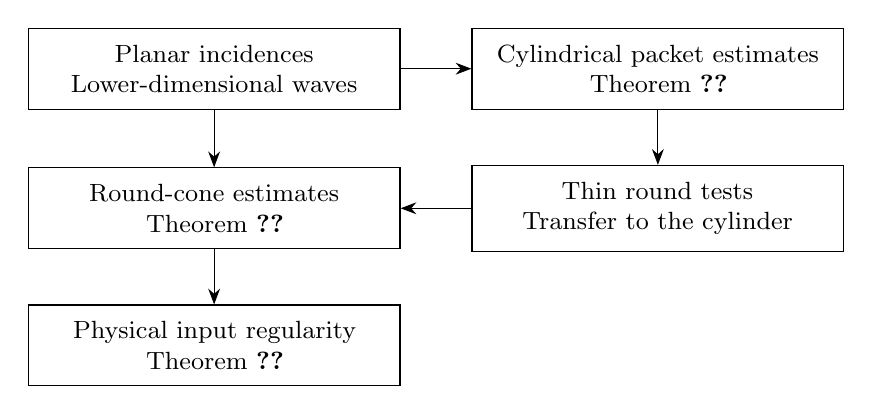
\begin{tikzpicture}[
 node distance=7mm and 9mm,
 every node/.style={font=\small,align=center},
 result/.style={draw,inner sep=6pt,text width=43mm},
 >={Stealth[length=2mm]}]
 \node[result] (inputs) {Planar incidences\\Lower-dimensional waves};
 \node[result,right=of inputs] (cylinder) {Cylindrical packet estimates\\Theorem~\ref{thm:cylinder}};
 \node[result,below=of cylinder] (transfer) {Thin round tests\\Transfer to the cylinder};
 \node[result,left=of transfer] (round) {Round-cone estimates\\Theorem~\ref{thm:round}};
 \node[result,below=of round] (physical) {Physical input regularity\\Theorem~\ref{thm:main}};
 \draw[->] (inputs)--(cylinder);
 \draw[->] (cylinder)--(transfer);
 \draw[->] (transfer)--(round);
 \draw[->] (inputs)--(round);
 \draw[->] (round)--(physical);
\end{tikzpicture}
\caption{Dependencies of the main estimates. Arrows indicate which
estimates are used in subsequent arguments.}
\label{fig:dependencies}
\end{figure}

\begin{samepage}
The principal technical steps are the extremal reduction with compatible
shears, the phase-name calculus, and the uniform transfer of wave packets
on thin gaps. These intermediate results are formulated for the packet
models considered here, independently of the final frequency summation.
Throughout,
finite operator stacks and polynomial cutoff bounds are fixed before
taking a scale limit; Section~\ref{sec:framework} specifies the order of
all subsequent limits.
\par
\end{samepage}

\clearpage
\tableofcontents
\clearpage

\section{Scales, energies, and limiting arguments}
\label{sec:framework}

The arguments below compare experiments whose parameters and probability
spaces vary with scale.  This section records the meaning of those
comparisons.  It does not assert that a geometrically defined
subexperiment is admissible: its support, regularity, and operator bounds
must be checked in the section where it is constructed.

\subsection{Fixed setups and exponent bounds}

We use dyadic scales $s=2^{-n}$ tending to zero.  A depth $a$ represents
the scale $s^a$.  Replacing it by the nearest dyadic scale changes a
positive quantity by a bounded factor and hence changes its normalized
logarithm by $O(1/\log(1/s))$.  Width exponents and growth exponents have
opposite sign conventions:
\[
 \operatorname{width\ exponent}(r)=\frac{\log r}{\log s},
 \qquad
 \operatorname{growth\ exponent}(B)=\frac{\log B}{\log(1/s)}.
\]
The growth exponent of a zero quantity is $-\infty$.

\begin{definition}[Fixed polynomial setup]\label{def:fw-setup}
A fixed polynomial setup specifies all structural constants, the finite
upper bounds on powers of $s^{-1}$ occurring in its hypotheses, and a
finite bound on the number of operations along each branch.  These data
are fixed before $s\to0$.  A sequence in this setup may have parameters,
operators, measures, and Hilbert spaces depending on $s$, provided the
specified bounds hold uniformly along the sequence.

An error $r_s$ is negligible relative to a positive reference quantity
$a_s$ if, for every $N>0$,
\[
 |r_s|\le C_N s^N a_s
\]
for all sufficiently small scales, with $C_N$ independent of scale.
For a family of choices at each scale, uniform negligibility means that
the same constants and scale thresholds work for every choice.  The
reference quantity is always specified; it may be an input energy or
an operator norm.  Polynomially many errors can be added without losing
negligibility when their reference quantities and polynomial bounds
are controlled uniformly.
\end{definition}

For a nonnegative functional $\mathcal B_s$, define its upper exponent
to be
\begin{equation}\label{eq:fw-upper-exponent}
 \Gamma=\sup_{\mathscr S}\ \sup_{(s_k,\mathcal E_k)}
 \limsup_{k\to\infty}
 \frac{\log\mathcal B_{s_k}(\mathcal E_k)}{\log(1/s_k)}.
\end{equation}
Here $\mathscr S$ ranges over fixed polynomial setups, and the inner
supremum ranges over admissible sequences in that setup with $s_k\to0$.
The particular model specifies which setups are allowed.  The finiteness
of $\Gamma$ must be proved for that model.

\begin{lemma}[Uniform bound within a fixed setup]
\label{lem:fw-uniform}
Suppose $\Gamma\in\R$ in \eqref{eq:fw-upper-exponent}.  Fix a family
$\mathcal A_s$ such that every sequence of choices
$\mathcal E_k\in\mathcal A_{s_k}$, $s_k\to0$, is admissible in one fixed
polynomial setup.  In particular, all negligible tail hypotheses are
uniform over this family.  For every $\eps>0$ there is $s_0>0$ such that
\begin{equation}\label{eq:fw-uniform-bound}
 \mathcal B_s(\mathcal E)\le s^{-\Gamma-\eps}
 \qquad(0<s<s_0,\ \mathcal E\in\mathcal A_s).
\end{equation}
If the functional is also uniformly bounded on this family at each of
the finitely many larger dyadic scales under consideration, then
\eqref{eq:fw-uniform-bound} holds on the entire scale range after
inserting a constant $C_{\eps,\mathscr S}$.
\end{lemma}

\begin{proof}
Failure of the first assertion provides $s_k\to0$ and
$\mathcal E_k\in\mathcal A_{s_k}$ with
$\mathcal B_{s_k}(\mathcal E_k)>s_k^{-\Gamma-\eps}$.
The resulting sequence is admissible in the fixed setup and has upper
exponent at least $\Gamma+\eps$, contradicting
\eqref{eq:fw-upper-exponent}.  For the second assertion, take the
maximum of the finitely many required constants at the remaining
scales and $1$.
\end{proof}

The constant in Lemma~\ref{lem:fw-uniform} may depend on every bound
fixed in Definition~\ref{def:fw-setup}.  It is not uniform when those
bounds grow along an outer approximation.  Conversely, a failure of an
estimate with a fixed positive exponent slack can be disproved within
one fixed setup, even when that setup was selected late in an outer
argument.

\begin{remark}[Small normalized pieces]\label{rem:fw-small-pieces}
Changing the reference energy can change a tail hypothesis.  For
example, an error negligible relative to $e$ is negligible relative to
$e'$ whenever $e'/e\ge s^C$ for some fixed $C$, but this implication
does not hold for arbitrary $e'>0$.  Applications to a collection of
subexperiments must therefore either verify the hypotheses relative
to each new energy, or use a direct estimate on pieces with
superpolynomially small energy.  No uniformity assertion in
Lemma~\ref{lem:fw-uniform} supplies this missing verification.
\end{remark}

\subsection{Energy and finite extraction}

Energy means a squared Hilbert norm.  Input energy at a time interval
means the energy before the evolutions and masks being estimated.
When a time interval is subdivided, its input is copied into its
descendants.  Consequently the sum of input energies over distinct
starting intervals need not be bounded by the original energy.
This sum will always be distinguished from the energy available to
one interval.

\begin{lemma}[Disjoint row restrictions and copies]
\label{lem:fw-energy}
Let $V:\mathcal H\to\mathcal K$ be an isometry and let $P_1,\ldots,P_N$
be mutually orthogonal projections on $\mathcal K$.  For
$g_j=V^*P_jVg$,
\begin{equation}\label{eq:fw-row-energy}
 \sum_{j=1}^N\norm{g_j}_{\mathcal H}^2
 \le\sum_{j=1}^N\norm{P_jVg}_{\mathcal K}^2
 \le\norm g_{\mathcal H}^2.
\end{equation}
If $\sum_jP_jVg=Vg$, then $\sum_jg_j=g$.
By contrast, for $N$ contractions $T_j$ applied to separate copies of
$g$, the general bound is only
$\sum_j\norm{T_jg}^2\le N\norm g^2$.
\end{lemma}

\begin{proof}
The adjoint $V^*$ has norm one.  Apply this fact to each $P_jVg$ and
then use orthogonality.  The reconstruction assertion follows from
$V^*V=\Id$.  The assertion about copies follows by applying
$\norm{T_jg}\le\norm g$ separately to each $j$.
\end{proof}

The projections in Lemma~\ref{lem:fw-energy} may be multiplication by
disjoint measurable row sets in a direct integral.  Their synthesized
images need not be orthogonal.  For the weighted sums used here, this
is accommodated by a norm inequality, not by an orthogonality claim.

\begin{lemma}[Extraction from finitely many classes]
\label{lem:fw-finite-extraction}
Let $q\ge1$, and suppose that a nonnegative functional $F$ satisfies
\[
 F(g_1+\cdots+g_N)^{1/q}
 \le\sum_{j=1}^N F(g_j)^{1/q}.
\]
Then some $j$ satisfies $F(g_j)\ge N^{-q}F(\sum_i g_i)$.
Consequently, if $N=N_s$ obeys
$\log N_s/\log(1/s)\to0$, passing to a maximizing class costs zero
growth exponent.  The same conclusion holds for a fixed finite
number of successive such extractions.  To use the conclusion for
a model exponent, each selected class must itself be admissible in
a fixed setup.

In particular, for linear maps $A_\lambda$ into Hilbert spaces and
positive weights $w_\lambda$,
\begin{equation}\label{eq:fw-cube-seminorm}
 F(g)=\sum_\lambda w_\lambda^{-1/2}\norm{A_\lambda g}^3
\end{equation}
has the required inequality with $q=3$.
\end{lemma}

\begin{proof}
The right side of the assumed inequality is at most
$N\max_jF(g_j)^{1/q}$.  Raising to the $q$th power proves the
extraction estimate.  Its logarithmic loss is
$q\log N_s/\log(1/s)$; finitely many such losses still tend to zero.
For \eqref{eq:fw-cube-seminorm}, $F(g)^{1/3}$ is the norm of
$(w_\lambda^{-1/6}A_\lambda g)_\lambda$ in the corresponding
$\ell^3$ sum of Hilbert spaces, and Minkowski's inequality applies.
For a countable label set, apply the inequality first to finite
subsets and then use monotone convergence.
\end{proof}

A separate elementary extraction will be used when energies are
already summable: if $0<E<\infty$, $A>0$, $a_j\ge0$, $e_j\ge0$,
$\sum_j e_j\le E$, and $\sum_j a_j\ge A$, then
$\sup_{j:e_j>0}a_j/e_j\ge A/E$, provided $a_j=0$ whenever $e_j=0$.
Indeed the contrary strict upper bound, multiplied by $e_j$ and
summed, contradicts the two hypotheses.  Any additional count or
regularity constraints on the chosen class require their own
discard estimates.

\subsection{Closure of exponent data}

For a finite list of positive quantities, exponent data are the limits
of their normalized logarithms along admissible sequences, when these
limits exist and are finite.  We may also take the closure of such data
in a fixed finite-dimensional Euclidean space.  This outer closure
permits a different fixed polynomial setup for each approximating
sequence.  It does not turn these sequences into one admissible
sequence with unbounded setup parameters.

\begin{lemma}[Extrema of bounded exponent data]
\label{lem:fw-closure}
Let $K\subset\R^{m+1}$ be a nonempty compact set of feasible limiting
data $(g,x_1,\ldots,x_m)$.  Set $G=\max_K g$, minimize $x_1$ on
$K\cap\{g=G\}$, and then successively minimize $x_j$ on the slice
where all preceding extrema are attained.  Every slice is nonempty
and compact, and every stated minimum is attained.

The attainment assertions, and nonemptiness and closedness of the
successive slices, remain valid for a possibly noncompact closed
set $K$ under the following hypotheses: $g$ has a finite supremum
and a bounded maximizing sequence in $K$, and each successive
coordinate has a finite infimum and a bounded minimizing sequence
within the preceding extremal slice.  This alternative does not
assert compactness of the slices.  A new coordinate may be added
to the tuple only after the required boundedness and feasibility
have been proved for the enlarged tuple.
\end{lemma}

\begin{proof}
A continuous coordinate function attains its extremum on a nonempty
compact set.  The set where that extremum is attained is closed in
the same compact set and is nonempty.  Induction proves the first
assertion.  For the alternative, pass first to a convergent
subsequence of the bounded maximizing sequence.  Closedness and
continuity attain the supremum of $g$.  At each subsequent step,
pass to a convergent subsequence of the stipulated bounded
minimizing sequence.  Closedness preserves feasibility, and
continuity of the coordinates preserves the preceding equalities
and attains the next infimum.  Each resulting slice is a nonempty
intersection of closed sets.
\end{proof}

\begin{remark}\label{rem:fw-extra-coordinate}
Boundedness of a new coordinate cannot be inferred from compactness
of previously chosen coordinates.  For example, the closure of the
projection of
$\{(p,c):c\ge1,\ p=1/c\}$ onto the $p$ axis contains $p=0$, although
the closure of the full set has no finite point with $p=0$.
Thus a geometric bound on the curvature cost at the already chosen
growth and mass exponents is an essential part of a curvature
minimization argument.
\end{remark}

\begin{lemma}[Strict improvement in a closure]
\label{lem:fw-strict-improvement}
Let $K\subset\R^{k+1}$ be a closed set of feasible data.  Suppose
that $c_0$ is the minimum of the last coordinate $c$ on the nonempty
slice $K\cap\{z=z_0\}$.  There cannot be data $(z_n,c_n)\in K$ with
$z_n\to z_0$ and $\limsup_n c_n<c_0$, provided $(c_n)$ is bounded
below and has a bounded subsequence.  In particular, a construction
contradicts minimality when its preceding exponents converge to the
specified extrema and its cost improves by a fixed positive amount
in the units of the constructed experiment.
\end{lemma}

\begin{proof}
Pass to a convergent subsequence of $(c_n)$.  Its limit $c$ is strictly
less than $c_0$.  Closedness places $(z_0,c)$ in the minimizing slice,
which is a contradiction.
\end{proof}

These lemmas assert neither an exactly extremizing input nor an
infinite chain of operators.  A construction at limiting exponent
data must be performed on approximating finite experiments.  The
estimates must then imply the asserted bounds on a convergent
subsequence of the finite tuples actually used.

\subsection{Ordered limits and changes of scale}

At a depth gap $h>0$, the new basic scale is $\delta=s^h$.  A factor
$s^{-\alpha}$ has growth exponent $\alpha/h$ in these new units.
Consequently a loss tending to zero in the original units is harmless
on a fixed gap, but it is harmless on shrinking gaps only after it has
been made $o(h)$.

All uses of mesh refinement or tangent gaps have the following order.
First fix the positive gap, the finite list of cuts and observations,
and all cutoff depths needed for that comparison.  In each fixed
polynomial setup take the scale limit.  Next make the preceding
approximation errors and mesh errors as small as required relative
to that fixed gap.  Only then shrink the gap or enlarge the finite
list.  When further tangent layers are used, their positive lengths
and required accuracies are fixed before the preceding tangent limit
is taken.  Each application of a model exponent is to an admissible
sequence at a fixed stage of these outer choices.

\begin{lemma}[Pullback of a strict exponent contradiction]
\label{lem:fw-pullback}
Let $\Gamma\in\R$ be an upper exponent as in
\eqref{eq:fw-upper-exponent}.  Suppose that, for each integer $m$, a
construction produces an admissible sequence in a fixed setup
$\mathscr S_m$ with upper exponent at least
$\Gamma+\tau-r_m$, where $\tau>0$ is fixed and $r_m\to0$.
Then such a construction is impossible.  The setup need not be
uniform in $m$.
\end{lemma}

\begin{proof}
Choose one fixed $m$ with $r_m<\tau/2$.  The sequence in
$\mathscr S_m$ then contradicts the definition of $\Gamma$.
\end{proof}

Having one favorable scale for each $m$ would not satisfy the
hypothesis of Lemma~\ref{lem:fw-pullback}.  For example, the quantities
$B_m(2^{-n})$, equal to $2^n$ when $n=m$ and equal to $1$ otherwise,
have upper exponent zero for every fixed $m$ but exponent one along
the diagonal $m=n$.  We will therefore use a diagonal of scales for
probability comparisons only after the necessary model estimates
with strict slack have been established in their fixed setups.

\subsection{Elementary probability comparisons}

All random variables below are evaluated under the probability law
specified at that point of the argument.  A conditional probability
may condition on a continuous variable or a sigma-algebra. We use
natural logarithms. Under a law $P$, for a finite-valued name $X$,
write
\[
 H_P(X\mid Y)=-\E_P\log P(X\mid Y).
\]
Relative entropy is
$\operatorname{KL}(P\Vert Q)=\int\log(dP/dQ)\,dP$ when $P\ll Q$,
and is $+\infty$ otherwise. Conditional mutual information is
\[
 I_P(X;V\mid Y)
 =\E_{P_Y}\operatorname{KL}
   \bigl(P_{X,V\mid Y}\Vert P_{X\mid Y}\otimes P_{V\mid Y}\bigr).
\]
This definition also permits continuous variables; when $X$ is finite,
it equals $H_P(X\mid Y)-H_P(X\mid V,Y)$. For $0<\rho<1$, the
scale-normalized quantities are $H_\rho=H_P/\log(1/\rho)$ and
$I_\rho=I_P/\log(1/\rho)$, with the law indicated when it changes.
For a finite-valued name $X$ and conditioning data $Y$, write
\begin{equation}\label{eq:fw-score}
 i_s(X\mid Y)
   =-\frac{\log\Prob(X\mid Y)}{\log(1/s)},
\end{equation}
where the conditional probability is evaluated at the sampled value
of $X$. Values on null events are immaterial. Thus
$H_s(X\mid Y)=\E_P i_s(X\mid Y)$: the score is random, whereas
entropy and mutual information are averaged quantities.

\begin{lemma}[Capacity tails]\label{lem:fw-capacity}
Suppose that, given $Y$, the variable $X$ has at most $N$ possible
values almost surely.  For every $u\ge0$,
\begin{equation}\label{eq:fw-capacity}
 \Prob\bigl\{\Prob(X\mid Y)<e^{-u}/N\bigr\}\le e^{-u}.
\end{equation}
If $N\le s^{-C}$ for a fixed $C$, then
$\Prob\{i_s(X\mid Y)>C+t\}\le s^t$ for $t\ge0$.
These normalized scores are uniformly integrable as $s\to0$.
In particular, convergence in probability to a finite constant
implies convergence of their expectations to that constant.
\end{lemma}

\begin{proof}
For each conditioning value, sum the conditional probabilities of
the at most $N$ values below $e^{-u}/N$, and then integrate.  This
proves \eqref{eq:fw-capacity} and its normalized version.  For $K>C$,
the tail integral identity gives
\[
 \E\bigl[i_s(X\mid Y)\mathbf 1_{\{i_s(X\mid Y)>K\}}\bigr]
 \le s^{K-C}\left(K+\frac1{\log(1/s)}\right).
\]
For $s\le1/2$ the right side tends to zero uniformly as $K\to\infty$.
This is uniform integrability; truncation at $K$ proves the final
assertion.
\end{proof}

The same estimate applies to a relative name with at most $N$
refinements after its parent has been included in the conditioning.
It does not require a bounded number of values for the conditioning
data.  When absolute names have unbounded capacity exponents along
an outer limit, the lemma supplies uniform integrability only for
the relative names whose capacities have been bounded.

\begin{lemma}[Stability under restriction]
\label{lem:fw-restriction}
Let $Q=P(\,\cdot\mid E)$, where $P(E)=q>0$, and let $X$ be a finite
name with arbitrary conditioning data $Y$.  If $q\ge s^\alpha$,
then, outside a set of $Q$-probability at most $2s^\tau$,
\begin{equation}\label{eq:fw-restriction}
 \abs{i_s^Q(X\mid Y)-i_s^P(X\mid Y)}\le\alpha+\tau
 \qquad(\tau>0).
\end{equation}
Consequently, restrictions with $q=s^{o(1)}$ preserve deterministic
limiting scores, provided their previous exceptional probabilities
are negligible relative to $q$.  On a gap with scale $s^h$, the
corresponding condition is $\log(1/q)=o(h\log(1/s))$ and all errors
are divided by $h$.
\end{lemma}

\begin{proof}
For the marginal of any variable $W$, the likelihood ratio
$L_W=dQ_W/dP_W$ is $P(E\mid W)/q$, hence is at most $1/q$.
Moreover
$Q\{L_W<s^\tau\}\le s^\tau$ by integrating $L_W$ against $P_W$.
Apply these two facts to $W=(X,Y)$ and $W=Y$.  Except on the union
of the two exceptional sets, both ratios belong to
$[s^\tau,s^{-\alpha}]$.  The conditional likelihood ratio is
$L_{(X,Y)}/L_Y$, so it belongs to
$[s^{\alpha+\tau},s^{-\alpha-\tau}]$.
Taking logarithms proves \eqref{eq:fw-restriction}.
An old exceptional event of $P$-probability $r$ has $Q$-probability
at most $r/q$, proving the stated qualification and the consequences.
\end{proof}

\begin{lemma}[Negligible information and positive restrictions]
\label{lem:fw-information}
Let $U,V$ be finite names, with arbitrary conditioning data $Y$.
Put $L=\log(1/s)$ and
\[
 j=\log\frac{P(U\mid V,Y)}{P(U\mid Y)}.
\]
Then $P\{j<-r\}\le e^{-r}$ for $r\ge0$, and
$\E j=I_P(U;V\mid Y)$.  If $I_P(U;V\mid Y)=o(L)$, then
$j/L\to0$ in probability.  If $Q=P(\,\cdot\mid E)$ and
$P(E)\ge q_0>0$, then
\begin{equation}\label{eq:fw-information-restriction}
 I_Q(U;V\mid Y)
 \le\frac{I_P(U;V\mid Y)+\log2}{q_0}.
\end{equation}
In particular such restrictions preserve $o(L)$ information budgets.
No such conclusion is asserted for arbitrary events of probability
$s^{o(1)}$.
\end{lemma}

\begin{proof}
Condition on $Y$ and compare the joint law of $(U,V)$ with the
product of its conditional marginals.  At actual samples their
likelihood ratio is $e^j$, so integrating over the set where it is
less than $e^{-r}$ proves the tail bound.  Therefore
$\E(j_-)\le1$, while the definition of conditional mutual
information gives $\E j=I_P(U;V\mid Y)$.  It follows that
$\E(j_+)\le I_P(U;V\mid Y)+1$.  Markov's inequality and the negative
tail bound prove convergence in probability after division by $L$.

Let $B=\mathbf 1_E$.  The chain rule gives
\[
 I_P(U;V\mid Y,B)
 \le I_P(U;V,B\mid Y)
 \le I_P(U;V\mid Y)+H_P(B\mid V,Y)
 \le I_P(U;V\mid Y)+\log2.
\]
The left side is the average, over the two values of $B$, of the
corresponding conditional mutual informations.  Its contribution
from $B=1$ is $P(E)I_Q(U;V\mid Y)$, proving
\eqref{eq:fw-information-restriction}.
\end{proof}

The elementary comparisons in this subsection refer to actual laws
and finite lists of names.  Later score limits may be obtained from
joint weak subsequences of those finite lists; no convergence of
conditional sampling kernels is required or asserted.  Extending
the limits to a dense set of depth queries requires the specific
nesting and list bounds proved for those names.  In particular,
these probability lemmas neither couple input and output packet
marginals through a quantum mask nor transfer a profile between
different measuring laws without a separate argument.

\section{Cylinder experiments and extremal configurations}
\label{sec:cylinder}

This section defines the two cylinder models and constructs the configurations
used in the cylinder estimates.  A state is measured by its squared Hilbert
norm.  Time subdivision copies that state into its descendant intervals;
it does not divide its energy among them.  This distinction explains the
growth factor in the normalization below.

\subsection{States, tests, and assignments}

Fix $0<\eta<1$ and $s=2^{-n}$.  A cut of length $\ell=2^{-k}$, with
$0\le k\le n$, consists of the dyadic subintervals of $[0,1)$ of that
length.  The final cut has length $s$ and contains exactly $s^{-1}$
intervals.  We measure an interval
at its left endpoint $T$.  There are finitely many operator cuts, in
nonincreasing order of length; repeated cuts are permitted.  Their number
is bounded on each polynomial setup.  Every child receives the freely
evolved state of its parent, with the operators specified on that branch.

The exact base index is $F=(X,B,Y)$, with
\begin{equation}\label{cyl:base-flow}
 B_T=B+TX,\qquad Y_T=Y+TX^2.
\end{equation}
Additional exact indices range over standard Borel spaces; arbitrary
separable Hilbert multiplicities are allowed. All integrals and squared
norms include these indices. One may equivalently use a measurable
direct integral of separable Hilbert spaces over such an index space.

\begin{definition}[Cylinder states]\label{cyl:def-states}
In the \emph{classical cylinder}, $(N,D)$ is another exact index,
$D_T=D+TN$, and free evolution leaves the state unchanged in these moving
coordinates.  In the \emph{hybrid cylinder}, $H>0$ is fixed, there is an
exact index $\sigma\in[1,2]$, and a fiber state belongs to
$L^2(\R_D;\mathcal H)$.  Its free propagator $U_t^{H,\sigma}$ is
\[
 \widehat{U_t^{H,\sigma}g}(p)
       =e^{-itHp^2/(2\sigma)}\widehat g(p).
\]
At length $\ell$, set
\[
 d_\ell=(H/\ell)^{1/2},\qquad q_\ell=(H\ell)^{1/2},
 \qquad
 \phi_{D,N}^{\ell,\sigma}(z)
  =(\pi q_\ell^2)^{-1/4}
    e^{-(z-D)^2/(2q_\ell^2)+i\sigma Nz/H}.
\]
The analysis operator is
\[
 (V_\ell g)(D,N)=\ip{g}{\phi_{D,N}^{\ell,\sigma}},
 \qquad d\nu_\sigma(D,N)=\frac{\sigma}{2\pi H}\,dD\,dN.
\]
For the classical model, $V_\ell=\Id$ and $d_\ell=0$.
An admissible operator at a cut is $V_\ell^*MV_\ell$, where $M$ is a
measurable pointwise contraction on the multiplicity space and preserves
all exact indices.  The row measure $\mu_I$ is the squared norm of the
analyzed state, possibly restricted by row assignments.
\end{definition}

With the Fourier normalization of Section~\ref{sec:introduction},
Plancherel in $N$ gives
\[
 \int_\R\abs{\ip{g}{\phi_{D,N}^{\ell,\sigma}}}^2
                   \frac{\sigma\,dN}{2\pi H}
 =\int_\R\norm{g(z)}_{\mathcal H}^2
             (\pi q_\ell^2)^{-1/2}e^{-(z-D)^2/q_\ell^2}\,dz.
\]
Integration in $D$ proves $V_\ell^*V_\ell=\Id$.  In particular, every
admissible operator is a contraction.  The packet parameter $D$ in the
hybrid model is an observation coordinate, not an exact classical index.

\begin{definition}[Cylinder tests]\label{cyl:def-test}
A test $Q$ at $(T,\ell)$ has widths $r>0$, $f\ge d_\ell$, with $f>0$.
For a hybrid row observed at the cut $T$, $D_T$ in the following
inequalities denotes its instantaneous analyzed center $D$, not an
exact classical trajectory. The test is specified by
\begin{gather}
 |X-x|\le r,\qquad |B_T-b|\le\ell r,\qquad
 |Y_T-y-2x(B_T-b)|\le\ell r^2,\label{cyl:base-test}\\
 |N-c-\alpha X-\beta(T)X^2-K(Y_T-2XB_T)|\le f,
 \label{cyl:velocity-test}\\
 |D_T-d-\alpha B_T-\beta(T)Y_T+KB_T^2|\le\ell f.
 \label{cyl:position-test}
\end{gather}
All centers and coefficients are real.  Extend the coefficients by
\[
 \beta(t)=\beta(T)+(t-T)K,\qquad d(t)=d+(t-T)c.
\]
The test weight is $w(Q)=r^{3+\eta}f^{1-\eta}$.  A row measure is
$\kappa$-regular if $\mu(Q)\le\kappa w(Q)$ for every admissible test.
\end{definition}

If the expressions subtracted from $N,D_T$ in
Equations~\eqref{cyl:velocity-test}--\eqref{cyl:position-test} are
$A(F)$ and $S_t(F)$, respectively, direct differentiation gives
$\partial_t A=0$ and $\partial_t S_t=A$.  Also
\begin{equation}\label{cyl:derivative}
 P(F)=\alpha+2\beta(t)X-2KB_t
\end{equation}
is independent of $t$.

An assignment to the final cut is a family of nonnegative row measures
$\mu_\lambda\le\mu_I$, each supported on a test $Q_\lambda$ at its own
interval, such that $\sum_{\lambda\text{ at }I}\mu_\lambda\le\mu_I$.
Fractional assignments are allowed.  Put $m_\lambda=\mu_\lambda(Q_\lambda)$
and $w_\lambda=w(Q_\lambda)$.  If $e>0$ is the root energy and the root
row measure is $\kappa$-regular, define
\begin{equation}\label{cyl:functional}
 \mathcal B_s
  =\frac{s^{-1/2}}{e\sqrt\kappa}
           \sum_\lambda\frac{m_\lambda^{3/2}}{\sqrt{w_\lambda}}.
\end{equation}
The sum includes all final intervals.  Bounded enlargements of the defining
inequalities are interchangeable with a bounded change of the weight:
enlarge $r,f$ by fixed constants or cover by finitely many translates.

\subsection{Cutoffs and localization}

\begin{definition}[Polynomial cylinder setup]\label{cyl:def-setup}
The quantities $e/\kappa,\kappa/e$ and, in the hybrid case, $H,H^{-1}$
are bounded by fixed powers of $s^{-1}$.  The initial base support lies in
a box of fixed-power size.  The initial normal phase has negligible mass
relative to $e$ outside such a box.  The marginal base density and the
joint density in $(X,B,Y,N,D)$ are bounded by $e$ times a fixed power of
$s^{-1}$, with respect to Lebesgue measure.  Negligibility is uniform
within each family to which an exponent bound is applied.  All these
powers, and the bound on the number of operators on a branch, are fixed
before $s\to0$.
\end{definition}

The exponent closure may use successively larger fixed powers, in the
ordered sense specified in the framework.  It never replaces the inner
scale limit by isolated scales with increasing cutoff powers.

\begin{lemma}[Symmetries and Gaussian localization]\label{cyl:localization}
The models are invariant under translations, base boosts, dilation in
base units $(r,r,r^2)$, normal dilation, affine time normalization, and
subtraction of one common normal shear of
Equations~\eqref{cyl:velocity-test}--\eqref{cyl:position-test}.  All
operators and assignments must be transformed with the state.

For $\ell'\le\ell$, $|t|\le C\ell$, and fixed $\eps>0$, the hybrid
frame transfer is negligible in operator norm outside
\begin{equation}\label{cyl:correspondence}
 |N'-N|\le s^{-\eps}d_{\ell'},\qquad
 |D'-D-tN|\le s^{-\eps}q_\ell.
\end{equation}
This remains true along any fixed finite stack of masks and after summing
over a polynomial number of intervals.  At a repeated cut, synthesis and
reanalysis of a restricted $\kappa$-regular row measure produce a
$C_\eta\kappa$-regular measure.  The same assertion holds for truncated
families of tests whenever the normal enlargements in the proof belong
to that family or are covered by translates belonging to it.
\end{lemma}

\begin{proof}
A base boost replaces $X$ by $X-x_0$ and replaces the last base position
by its appropriate linear tilt in $B_t$; Equation~\eqref{cyl:base-flow}
then has the same form.  A common normal shear subtracts
$a(F)$ from velocity and $b(F)+ta(F)$ from position.  On each hybrid
fiber it is a Weyl translation, and the free propagator intertwines the
two translations up to a scalar phase.  The scalar phase can be included
in the conjugated mask.  If a time interval of length $L$ is normalized
to unit length, positions are divided by $L$, velocities are unchanged,
and $H$ becomes $H/L$.  Dividing normal coordinates and velocities by
$F_0$ changes $H$ to $H/F_0^2$.  Dividing base coordinates by
$(r_0,r_0,r_0^2)$ and normal coordinates by $F_0$ divides all weights
by $A=r_0^{3+\eta}F_0^{1-\eta}$ and multiplies the regularity constant
by $A$.  Energy is preserved by the corresponding unitary coordinate
changes.  Thus Equation~\eqref{cyl:functional} is unchanged.

The scalar transfer kernel is
$\ip{U_t^{H,\sigma}\phi_{D,N}^{\ell,\sigma}}
          {\phi_{D',N'}^{\ell',\sigma}}$.
Free propagation changes the first packet's position width to at most
$Cq_\ell$, since $|t|H/q_\ell\le Cq_\ell$, and leaves its Fourier
width comparable to $q_\ell^{-1}$.  Integrating two Gaussians, in physical
space for the position difference and in Fourier space for the momentum
difference, gives an upper bound of the form
\[
 C_s\exp\left[-c\left(
       \frac{|D'-D-tN|^2}{q_\ell^2}
       +\frac{|N'-N|^2}{d_{\ell'}^2}\right)\right],
\]
where $C_s$ and the Schur integration volumes have only fixed-power
costs on the setup.  Each of the two separate Gaussian bounds implies
the displayed joint bound after reducing $c$.  Schur's test therefore
makes the discarded kernel smaller than every power of $s$.  A finite
product and a polynomial sum preserve this conclusion.  If no chain of
the correspondences connects two row sets, the operator between those
sets is negligible; this statement does not require a positive-kernel
description of its main part.

At a repeated cut the absolute kernel is exactly
\[
 \exp\left(-\frac{(D-D')^2}{4q_\ell^2}
           -\frac{\sigma^2(N-N')^2}{4d_\ell^2}\right).
\]
Its Schur norms are bounded independently of $H,\ell$.  Cauchy--Schwarz
against this kernel bounds output energy on a test by a Gaussian-weighted
sum of input energies on its normal enlargements.  Since $f\ge d_\ell$
and $\ell f\ge q_\ell$, the enlargement in the $j$th Gaussian shell
is obtained by multiplying the normal width by $C(1+j)$.  The resulting
regularity bound is
$C\kappa w(Q)\sum_{j\ge0}e^{-cj^2}(1+j)^{1-\eta}$.
Exact base indices are never mixed.  This proves the last assertion.
\end{proof}

\begin{lemma}[Polynomial test reduction]\label{cyl:polynomial-tests}
At every stage of a polynomial setup, the base and normal cutoff and
density conditions hold with enlarged fixed powers.  To any prescribed
polynomial regularity floor or error tolerance, it suffices to test
widths, reciprocal widths, and absolute test parameters bounded by
fixed powers.  Discarding output tests whose mass-to-weight ratio is
below $\rho$ costs at most $\sqrt\rho$ times total assigned mass in
the cubic readout, independently of the number of tests.
\end{lemma}

\begin{proof}
Base indices move exactly and masks are contractions on each fiber.
In the hybrid model, the pointwise packet bound gives a joint phase
density at most $C H^{-1}$ times the marginal base energy density.
Lemma~\ref{cyl:localization} propagates normal tails.  The density and
base-support bounds give, uniformly in shear parameters,
\begin{equation}\label{cyl:volume-bound}
 \mu(Q)\le e s^{-C}\min(r^4,1)\min(f^2,1).
\end{equation}
For $f\le1$ use joint density, and for $f>1$ use marginal base density.
Dividing by $r^{3+\eta}f^{1-\eta}$ shows that either sufficiently small
width gives an arbitrarily small prescribed power: the factors are
$r^{1-\eta}$ and $f^{1+\eta}$, respectively.  If neither width is small
and one is sufficiently large, the total-energy bound suffices.

We record an elementary sublevel estimate to handle coefficients.  For a
nonzero real polynomial $Q$ of degree at most two in $d\le3$ variables, on a
fixed cube,
\begin{equation}\label{cyl:sublevel}
 \vol\{\abs Q\le\rho\norm{Q}_{\mathrm{coeff}}\}
       \le C_d\rho^{2^{-d}},\qquad 0<\rho<1.
\end{equation}
Here the coefficient norm is the maximum absolute coefficient.  In one
variable, three points in a set of measure $m$, separated by at least
$cm$, and Lagrange interpolation show
$\norm Q_{\mathrm{coeff}}\le C\rho\norm Q_{\mathrm{coeff}}/m^2$.
For the induction, write $Q$ as a polynomial in the last variable and
choose a coefficient polynomial with coefficient norm equal to
$\norm Q_{\mathrm{coeff}}$.  Outside the set where this coefficient is
smaller than $\rho^{1/2}\norm Q_{\mathrm{coeff}}$, the one-dimensional
bound is $C\rho^{1/4}$; the exceptional base set has measure at most
$C\rho^{2^{-d}}$ by induction.  This proves
Equation~\eqref{cyl:sublevel}, with harmless changes of constants.

For widths in a fixed polynomial range, discard negligible normal tails
and clip base centers to a fixed-power box.  The two normal shear
polynomials have coefficient norm comparable, by a fixed-power change
of coordinates, to the maximum of $|c|,|d|,|\alpha|,|\beta(T)|,|K|$.
If that maximum is sufficiently large, at least one of their simultaneous
sublevel conditions has arbitrarily small prescribed polynomial volume
by Equation~\eqref{cyl:sublevel}.  The density bound handles its mass.
Finally,
$m_\lambda^{3/2}/\sqrt{w_\lambda}
 =m_\lambda\sqrt{m_\lambda/w_\lambda}$, so small ratios are summed
against assigned mass, not against label cardinality.
\end{proof}

We shall also use the following convention for very small pieces.  An
experiment with input energy $e'$ and prescribed regularity $\kappa'$
satisfies the direct estimate
\begin{equation}\label{cyl:tiny-energy}
 \mathcal B_s\le s^{-3/2}
       \max_\lambda\sqrt{e'/(\kappa'w_\lambda)}.
\end{equation}
Indeed $m_\lambda\le e'$ and total assigned mass is at most $s^{-1}e'$.
For uniform application to a family of pieces one uses a fixed threshold,
not a scale-dependent notion of smallness.  Let the old reference energy
be $e_0$, suppose the summed piece energies have a polynomial bound
relative to $e_0$, and let $w_{\min}$ be a common polynomial lower bound
for relevant output weights.  Pieces with $e_G\le s^A e_0$ have total
cubic readout at most
\[
 s^{-1}w_{\min}^{-1/2}\sum_G e_G^{3/2}
 \le s^{-1}w_{\min}^{-1/2}(s^A e_0)^{1/2}\sum_Ge_G.
\]
Taking the fixed $A$ sufficiently large makes this smaller than any
specified polynomial comparison scale.  Every remaining piece has
uniform cutoff and negligible-tail bounds relative to its own energy,
after enlarging fixed powers.  Prescribed regularity constants in the
applications are also polynomial relative to $e_0$, so both energy to
regularity ratios are polynomial.  The uniform model exponent from
Lemma~\ref{lem:fw-uniform} therefore applies to this remaining family.

\subsection{The extremal exponent and ordinary splitting}
\label{cyl:extremal-exponent}

For each cylinder model, take the supremum of the upper
$\log_{1/s}$-exponents of Equation~\eqref{cyl:functional} over its
polynomial setups. Denote these exponents by $\Gamma_{\mathrm{cl}}$
and $\Gamma_{\mathrm{hyb}}$. The uniform interpretation on each fixed
setup, and all closure extrema below, use the ordered conventions of
Section~\ref{sec:framework}.

\begin{theorem}[Cylinder exponent bound]\label{thm:cylinder}
For the classical and hybrid cylinder experiments with the
regularity weight parameter $0<\eta<1$,
\[
 \Gamma_{\mathrm{cl}}\le\eta/2,
 \qquad \Gamma_{\mathrm{hyb}}\le\eta/2.
\]
\end{theorem}

The proof occupies the rest of this section and
Sections~\ref{sec:low}--\ref{act:section}. We first bound the growth
exponent, then study experiments whose cubic readout approaches it.
Any ordinary regularity split that preserves this extremal growth forces its
energy and regularity bounds to be sharp at the level of exponents.
We then choose the retained tests with compatible shears and describe
how their widths vary with depth. These properties supply the geometric
input for the entropy argument.

Fix either model and write $\Gamma$ for its exponent. We begin by proving
that it is finite.

\begin{lemma}[One-time bound]\label{cyl:one-time}
For a polynomial test at a cut of length $\ell$, an experiment with
$\kappa$-regular input satisfies
\begin{equation}\label{cyl:one-time-bound}
 \mu_I(Q)\le s^{-o(1)}\kappa w(Q)\ell^{1+\eta/2}.
\end{equation}
Consequently $\Gamma$ is finite.
\end{lemma}

\begin{proof}
Subtract the test's shear.  Backward packet correspondences place its
normal predecessors in root conditions of width $s^{-o(1)}f$, since
every intervening $d_{\ell'}$ is at most $d_\ell\le f$.  Split its
$X$-range into $O(\ell^{-1/2})$ intervals of width $r\sqrt\ell$.
For each such interval, backflow of the two base position conditions is
covered by a bounded number of root tests of base width $r\sqrt\ell$:
the horizontal error is $O(r\sqrt\ell)$ and the curvature error in the
tilted coordinate is $O(\ell r^2)$.  Summing their weights gives
\[
 O(\ell^{-1/2})(r\sqrt\ell)^{3+\eta}f^{1-\eta}
       =O(1)w(Q)\ell^{1+\eta/2}.
\]
Contraction on this predecessor region and
Lemma~\ref{cyl:localization} prove the claim; polynomial test bounds
absorb the negligible errors.  Total output mass is at most $s^{-1}e$,
so Equation~\eqref{cyl:one-time-bound} also gives
$\mathcal B_s\le s^{-1+\eta/4-o(1)}$.
\end{proof}

Suppose henceforth that $\Gamma>0$.  Dyadic binning of widths and
mass-to-weight ratios produces extremizing families with common widths
and
\begin{equation}\label{cyl:pd}
 \frac{m_\lambda}{\kappa w_\lambda}=s^{p+o(1)},\qquad
 \sum_\lambda m_\lambda=e s^{-d+o(1)},\qquad
 \Gamma=d+\frac{1-p}{2},\quad p\ge1,\quad0<d\le1.
\end{equation}
Thus $p$ measures the decay of each assigned mass relative to its
regularity bound, whereas $d$ measures the total mass read across the
copied time intervals. The identity for $\Gamma$ follows by substituting
the two mass relations into Equation~\eqref{cyl:functional}.
Negligible ratio classes are first removed by
Lemma~\ref{cyl:polynomial-tests}; there are subpower many remaining bins.
Choose the smallest possible $p=p_0$ in the closure of these extremal
data. This selects the largest normalized assigned mass-to-weight ratios
compatible with extremal growth. In particular $p<3$. The output label
family then has
\begin{equation}\label{cyl:terminal-count}
 \sum_{\lambda\ \mathrm{allowed}}w_\lambda
       \le(e/\kappa)s^{-(p+d)+o(1)}.
\end{equation}

\begin{lemma}[Regularity peeling]\label{cyl:peeling}
At a fixed cut, a state can be decomposed coherently into subpower many
row projections followed by synthesis.  Apart from a remainder at any
prescribed polynomial floor, each level has a number $b>0$ with the
following properties.  Its raw row measure is $O(b)$-regular; it has
disjoint assignments to tests of masses between $b w$ and $C b w$; if
$z$ is its total raw energy, their total weight is at most $z/b$.
The synthesized energies sum to at most $z$, and each synthesized state
is $s^{-o(1)}O(b)$-regular.  Levels may be subdivided by subpower many
statistics without altering these upper bounds.
\end{lemma}

\begin{proof}
Start above the fixed-power upper bound furnished by
Lemma~\ref{cyl:polynomial-tests}, and descend through dyadic thresholds.
At threshold $b$, remove the entire remaining part of a test whenever its
mass exceeds $bw$.  Its mass is at most $2bw$, by regularity of the
preceding remainder.  A polynomial lower bound on the allowed weights
makes the removal procedure finite by total mass.  The union removed at
this threshold is dominated by that preceding remainder and is therefore
$2b$-regular.  The unremoved measure is $b$-regular.  Continue to the
prescribed floor.  The removed row sets are disjoint and their projections
sum to the identity.  Synthesis is a contraction, and
Lemma~\ref{cyl:localization} gives post-synthesis regularity.

For a fixed terminal assignment, its cubic readout to the power $1/3$
is a weighted $\ell^3$ norm of Hilbert norms.  Hence coherent decomposition
costs at most a fixed power of the number of levels by the triangle
inequality.  That number is subpower, and at least one level preserves
any extremal output exponent.
\end{proof}

\begin{proposition}[Saturation of a preserving split]\label{cyl:split-saturation}
Retain the terminal family in Equation~\eqref{cyl:terminal-count}.
After any finite sequence of inserted operators or splittings that
preserves its extremal exponent, every dominant homogeneous terminal
class again has the exponents $p,d$ in Equation~\eqref{cyl:pd}.
Suppose a non-remainder level supplied by Lemma~\ref{cyl:peeling} at
depth $a\in(0,1)$ preserves this exponent. Let $b$ be its peeling
threshold and $z$ its total raw energy, summed over the intervals of
that cut. Then
\begin{equation}\label{cyl:split-benchmarks}
 b=\kappa s^{pa+o(1)},\qquad
 z=e s^{-da+o(1)}.
\end{equation}
The summed post-synthesis energy has the same exponent as $z$.
The conclusion holds for a further sublevel that preserves the output.
\end{proposition}

\begin{proof}
A new terminal class has $p'\ge p$ by minimality and
$d'=\Gamma+(p'-1)/2$.  Its assigned mass and the fixed weight count imply
$p'+d'\le p+d$.  Both inequalities force $p'=p$ and $d'=d$.

For a non-remainder peeling level at $\ell=s^{a+o(1)}$, apply the prefix
exponent to its raw heavy-test assignments.  Lemma~\ref{cyl:peeling}
gives
\begin{equation}\label{cyl:prefix-split}
 \ell^{-1/2}z\sqrt{b/\kappa}
       \le \ell^{-\Gamma-o(1)}e.
\end{equation}
The tail exponent, applied separately to each interval and summed with
its own post-energy, gives cubic readout at most
\[
 (s/\ell)^{1/2-\Gamma-o(1)}z\sqrt b.
\]
Combining this with Equation~\eqref{cyl:prefix-split} recovers the full
extremal upper exponent.  Since the chosen level preserves that exponent,
both estimates, and the synthesis energy bound, must be saturated in
exponent.  The floor remainder is negligible: its summed input energy
is at most $\ell^{-1}e$, and a sufficiently small regularity floor makes
the tail readout smaller by a fixed power.

Write $b/\kappa=s^{P+o(1)}$.  The saturated prefix has mass-to-weight
exponent $P/a$, so minimality implies $P/a\ge p$.  For the tail first
select a homogeneous dominant terminal mass class, then an interval
whose normalized readout is near maximal.  That tail realizes $\Gamma$
in the closure and has mass-to-weight exponent $(p-P)/(1-a)$; hence
$(p-P)/(1-a)\ge p$.  The one-time bound bounds $P$ on the fixed gap, so
these are legitimate finite closure data.  Thus $P=pa$, and saturation
in Equation~\eqref{cyl:prefix-split} gives $z=e s^{-da+o(1)}$.

For a sublevel, use the unpartitioned level in the prefix argument.
It bounds the sublevel's raw energy from above.  The preserving tail
bounds its post-energy from below by the same exponent.  At the root,
the given input regularity and energy replace the prefix estimate.
At the last cut a repeated-cut regularity estimate replaces the tail.
\end{proof}

For later use put
\begin{equation}\label{cyl:benchmarks}
 \ell_i=s^i,\qquad E_i=e s^{-di},\qquad\kappa_i=\kappa s^{pi}.
\end{equation}
Depths and widths are dyadically rounded.  All exponent upper and lower
bounds below permit $s^{\mp o(1)}$ factors.  On a fixed gap $h>0$, these
are also vanishing losses in $\log_{s^h}$ units.

\subsection{Matched gates}

Ordinary splitting controls energy and regularity at successive cuts.
We now also align the shear frames of the retained tests. This compatibility
will allow a later phase name to be compared with earlier names along a
retained path.

A \emph{documented gate} is a row projection followed by synthesis,
whose retained rows are partitioned among tests.  A retained row belongs
to its assigned test; the associated test is its documented label.
The last gate is simply the final assignment and need not be synthesized.
Statements about reachability refer to chains of
Equation~\eqref{cyl:correspondence} through the fixed retained
mask/test row sets. They do not impose the original state's
positive-norm support at intermediate cuts, which need not persist
after an input restriction. They assert geometric incidence, not a
joint probability law for the input and output of a quantum operator.

\begin{proposition}[Matched-chain construction]\label{cyl:matched-chain}
On any fixed finite depth mesh $0\le i_0<\cdots<i_b=1$, an extremizing
family can be modified by finitely many masks, preserving its terminal
exponent on the original label family, so that the following hold.
\begin{enumerate}[label=\textup{(\roman*)}]
\item At depth $i$, the documented tests have common widths $r_i,f_i$
and total weight at most $s^{-o(1)}E_i/\kappa_i$.
\item Ordinary regularization may be imposed immediately before each
gate, in forward order, giving summed energy at most $s^{-o(1)}E_i$
and regularity at most $s^{-o(1)}\kappa_i$ in each interval.
\item The total mass read on the documented rows is at least
$s^{o(1)}E_i$.  This lower bound persists after any further restrictions
that preserve the terminal exponent and retain these gates in series.
\item If $j$ is the next mesh depth and $\delta=s^{j-i}$, then, for
$L_*=L_*(\eta)$ independent of the mesh,
\[
 \delta^{L_*}\lesssim r_i/r_j\le1,\qquad
 \delta^{L_*}\lesssim f_i/f_j\lesssim\delta^{-L_*}.
\]
On every connecting packet chain between the two documented labels,
\begin{equation}\tag{M}\label{eq:M}
 \begin{split}
 |\beta_i(T_i)-\beta_j(T_i)|+\ell_i|K_i-K_j|
       &\lesssim(f_j/r_j^2)\delta^{-L_*},\\
 |P_i(F)-P_j(F)|&\lesssim(f_j/r_j)\delta^{-L_*}.
 \end{split}
\end{equation}
These comparisons survive insertion of any fixed finite intervening
operator stack, with a sufficiently small correspondence truncation
exponent relative to the mesh gaps.
\end{enumerate}
\end{proposition}

We first prove the geometric estimate used in its construction.

\begin{lemma}[Two-shear intersection]\label{cyl:intersection}
Normalize one starting interval and the later test widths to
$\ell_i=r_j=f_j=1$, and put $\delta=\ell_j/\ell_i$.
Let $Q^-,\widetilde Q^-$ be two projected tests, with bounded base
footprints and normal widths $O(\delta^{-1})$.  At the first base center
let $M$ be the maximum of $1$ and the differences of $P,\beta(T_i),K$.
For a $\kappa_i$-regular starting measure,
\begin{equation}\tag{I}\label{eq:I}
 \mu(Q^-\cap\widetilde Q^-)
       \le s^{-o(1)}\delta^{-C}\kappa_i w_j/M.
\end{equation}
If every retained descendant label has mass at least
$\delta^D\kappa_iw_j$, then a fixed projected label has at most
$s^{-o(1)}\delta^{-C_D}M_0^{1-\eta}$ intersecting partners in the
shell $M\asymp M_0$.
\end{lemma}

\begin{proof}
Subtract the first shear and center its base chart.  The intersection
imposes, on bounded $(X,B,Y)$,
\[
 |\alpha X+\beta X^2+k(Y-2XB)+c'|\lesssim\delta^{-1},\qquad
 |\alpha B+\beta Y-kB^2+d'|\lesssim\delta^{-1},
\]
where $\max(1,|\alpha|,|\beta|,|k|)\asymp M$.
If $\max(|\beta|,|k|)\gtrsim M$, multiplying the first expression by
$\beta$ and subtracting $k$ times the second gives
\[
 |t^2+\alpha t+\mathrm{const}|\lesssim M\delta^{-1},
 \qquad t=\beta X-kB.
\]
On a dyadic shell $R\asymp\max(\sqrt M,|2t+\alpha|)$, its admissible
$t$-set lies in at most two intervals of length $O(M\delta^{-1}/R)$.
In the lowest shell the same conclusion follows from proximity to the
quadratic vertex.  Since $\max(|\beta|,|k|)\gtrsim M$, the horizontal
set is covered by $O(\delta^{-1}R)$ squares of side $1/R$.

In such a square use the coordinate $Y-2x_{\mathrm{cell}}B$.
After the vertical terms are removed, the horizontal derivatives of the
two expressions are $O(R+M/R)$, so their oscillation across the square
is $O(1)$ because $R\ge\sqrt M$.  At least one vertical coefficient has
size comparable to $M$.  Therefore
$O(\delta^{-1}R^2/M)$ vertical intervals of length $R^{-2}$ suffice.
The intersection is covered by
$O(\delta^{-2}R^3/M)$ Heisenberg base cells of width $O(1/R)$, together
with the first normal conditions enlarged by $O(\delta^{-1})$.
Regularity bounds their total mass by
\[
 C\delta^{-C}\kappa_i w_j
       \frac{R^3}{M}R^{-3-\eta}
       \le C\delta^{-C}\kappa_iw_j/M.
\]
There are only logarithmically many shells on a polynomial setup.

Otherwise $|\alpha|\asymp M$ and $|\beta|,|k|$ are sufficiently small
relative to $M$ on the bounded base box.  For fixed $Y$, the second
expression has a $B$ derivative comparable to $M$, and the first then
has an $X$ derivative comparable to $M$.  The volume is
$O(\delta^{-2}M^{-2})$.  Its Heisenberg neighborhood of width $1/M$
obeys the same estimate, since the expressions change only by a constant
there.  It can consequently be covered by
$O(\delta^{-2}M^2)$ cells of weight $O(M^{-3-\eta})$, proving the same
bound.  Bounded $M$ needs no subdivision.

For the partner count, every intersecting partner in the shell has its
whole projected footprint in a bounded enlargement of the first base
box, and in normal width $O(\delta^{-1}M_0)$ about the first shear.
This follows by extending the difference polynomials from an intersection
point across bounded base coordinates.  At each descendant time,
contraction and starting regularity bound the total mass of these
assigned rows by
$s^{-o(1)}\kappa_i w_j O(\delta^{-1}M_0)^{1-\eta}$.
Divide by the assumed mass per label and sum over at most $O(\delta^{-1})$
descendant times.
\end{proof}

\begin{proof}[Proof of Proposition~\ref{cyl:matched-chain}]
\textbf{Read mass at a gate.}
First observe that the asserted mass lower bound follows whenever the
gate and weight count have been constructed.  Insert an ordinary split
immediately after the gate in a thought experiment preserving the
terminal exponent.  Proposition~\ref{cyl:split-saturation} requires
summed post-energy $s^{o(1)}E_i$, and contraction bounds it by the raw
gate mass.  At the final cut use the fixed terminal count and minimality
of $p$.  At the root, repeated-cut regularity is $s^{-o(1)}\kappa$,
so reducing post-energy by a fixed power would lose the terminal exponent
by the full tail bound.

\paragraph{Removing incompatible rows.}
Construct the gates backwards.  Suppose the $j$-gate is fixed and set
$a=j-h$, $\delta=s^h$.  At $a>0$ make an ordinary preserving split;
at $a=0$ use the root state.  The resulting states $g_a$ have total
energy at most $s^{-o(1)}E_a$ and regularity at most
$s^{-o(1)}\kappa_a$.  At $j$ their row measure is at worst
$s^{-o(1)}\kappa_a$-regular by Lemma~\ref{cyl:one-time}.
Delete labels whose newly read mass is less than
$\delta^D\kappa_aw_j$.  Their total mass is at most
\[
 s^{-o(1)}\delta^D\kappa_a E_j/\kappa_j.
\]
After synthesis they remain $s^{-o(1)}\kappa_a$-regular.  Their tail
readout, relative to the required scale $E_j\sqrt{\kappa_j}$ at $j$,
therefore loses at least $\delta^{D-3p/2-o(1)}$.  Since $p<3$, an
absolute $D$ makes the deletion harmless.  At $j=1$, use the output
ratio bound directly.

Every retained descendant test projects to a starting test $Q^-_\lambda$
with base width $O(r_j)$ in $\ell_a$ position units and normal width
$O(\delta^{-1}f_j)$.  Base backflow follows from the quadratic identity;
normal backflow follows from Lemma~\ref{cyl:localization}, taking its
truncation exponent smaller than $h/10$.  Each such projected test
contains every predecessor on the allowed correspondence chains.
All label counts here are polynomial by their weight count and the
polynomial lower bound for $w_j$.

Call a starting row ambiguous if it lies in two projected tests with
$M>\delta^{-D_0}$.  Lemma~\ref{cyl:intersection}, its partner count,
and the $j$-gate weight count bound its total mass by
\[
 s^{-o(1)}E_j(\kappa_a/\kappa_j)
                  \delta^{-C}\delta^{\eta D_0}.
\]
Choose $D_0=D_0(\eta)$ large enough that this is smaller than $E_a$ by
a fixed power of $\delta$.  Restricted rows retain regularity after
synthesis, so their tail is negligible by the model exponent.  Remove
them and also rows belonging to no projected retained test.  The latter
have negligible transfer to the $j$-gate.  Both removals use one row
projection followed by synthesis, not successive assumptions about
disjointness of synthesized states.

\paragraph{Shear charts.}
Partition the remaining rows into charts $G$.  First record a lattice
Heisenberg base cell of width $r_j$.  Choose one attached test in a fixed
order and round its five shear data at that cell center: $\beta(T_a)$,
$K$, $P$, and its two normal values.  Round in normal units
\[
 f^*=\delta^{-D_*}f_j,\qquad D_*>D_0+2.
\]
The five data determine the polynomial by a triangular change of
coordinates.  Nonambiguity makes every attached test's data lie within
a bounded number of these rounded values.  Thus each $j$-label meets
only boundedly many charts.  In each chart, after subtracting the common
rounded shear, base and normal support are bounded in
$(r_j,f^*,\ell_a)$ units, and every attached $j$-test has bounded
coefficients in those units.

\paragraph{Full chart regularity.}
The charts now have compatible geometry. To apply the model exponent to
their synthesized states, we also need full regularity. The next peel gives
regularity on a bounded range of tests; the subsequent reanalysis,
smoothing, and cutoff estimates extend it to the full test family.

Within each chart perform a truncated peel: normalized widths belong to
$[\delta^{D_1},1]$, with the Planck floor retained, and normalized shear
coefficients have absolute value at most $\delta^{-D_1}$.  Centers are
unrestricted.  The physical weight multiplier is
$w^*=r_j^{3+\eta}(f^*)^{1-\eta}$.  Keep one density and width class
coherently across all charts; there are subpower many classes, so some
class preserves the output.  Let $b_*$ be its density bound, or its
floor if it is the remainder.  Then $b_*\le s^{-o(1)}\kappa_a$,
the raw mass in each chart is $O(b_*w^*)$, and the synthesized chart
energies satisfy $\sum_G e_G\le s^{-o(1)}E_a$.

We justify applying the full model exponent with regularity $b_*$ to
each chart.  Same-cut Gaussian reanalysis preserves its truncated
regularity: normal shell enlargements can be covered by translates at
unchanged widths and coefficients.  Smooth the input and the entire
subexperiment by independent base boosts, base position translations,
and the two normal translations, each of size $\delta^l$, where
$l>D_*+10$.  Retain the smoothing parameter as an exact auxiliary index.
These are exact symmetries.  The smallest attached output accuracy is
$\delta^{1+D_*}$, so assigned masses persist on bounded enlarged tests.
In normalized units the smoothed base and joint densities are at most
\[
 C\delta^{-5l} b_* w^*.
\]
This follows by averaging translations, whose coordinate Jacobians are
one, and using the raw chart mass bound.  Base support is bounded;
normal support outside $s^{-o(1)}$ is negligible by Gaussian tails.

Here are explicit choices showing that the fixed density cost disappears
from the regularity estimate.  Choose $D_2$ with
$(1-\eta)D_2>5l+1$.  Equation~\eqref{cyl:volume-bound} gives
\[
 \frac{\mu(Q)}{b_*w^*w(Q)}
 \le C\delta^{-5l}
 \frac{\min(r^4,1)\min(f^2,1)}{r^{3+\eta}f^{1-\eta}}.
\]
Thus any width below $\delta^{D_2}$ is harmless.  Widths above one are
handled by bounded base covering or, for the normal width, by dropping
the normal conditions and covering the $s^{-o(1)}$ normal support with
unit translates.  For widths in $[\delta^{D_2},1]$, choose $D_3$ so
that $2^{-3}D_3>5l+4D_2+1$.  Equation~\eqref{cyl:sublevel} makes tests
with a coefficient above $\delta^{-D_3}$ harmless, even after dividing
by their minimum weight $\delta^{4D_2}$.  All remaining tests pull back
under each jitter to permitted truncated tests, provided
$D_1>D_2+D_3+10$.  For them the original truncated regularity bound is
used directly and incurs no factor $\delta^{-5l}$.
This proves full regularity $s^{-o(1)}b_*w^*$ in normalized units.
Tiny-energy chart pieces use Equation~\eqref{cyl:tiny-energy}; the others
satisfy the polynomial setup relative to their own energy.

\paragraph{Saturation and induction.}
The model exponent and the bounded chart overlap now bound the coherent
cubic readout at $j$ by
\begin{equation}\label{cyl:chart-upper}
 s^{-o(1)}\delta^{1/2-\Gamma}\sqrt{b_*}\sum_Ge_G.
\end{equation}
Indeed, for a label reached by at most $C$ chart states,
$\norm{\sum_{G=1}^Cv_G}^3\le C^2\sum_G\norm{v_G}^3$.
The already established read-mass lower bound and weight count, by
H\"older, give the lower bound
\[
 s^{o(1)}E_j\sqrt{\kappa_j}
  =s^{o(1)}\delta^{1/2-\Gamma}E_a\sqrt{\kappa_a}.
\]
Consequently $b_*=\kappa_a s^{o(1)}$, and the floor remainder can be
excluded.  Use the heavy tests in the selected truncated level as the
new documented labels.  Their total weight is at most
$s^{-o(1)}E_a/\kappa_a$.  Their truncated widths and coefficients,
together with chart compatibility, give the width bounds and
Equation~\eqref{eq:M}.  The constants depend only on the choices above,
hence only on $\eta$, not on the number of mesh steps.  Any reachable
$j$-test is attached to the actual supporting row of the new gate; no
assertion about its mass in an earlier state is used.

This completes the backward induction.  Finally insert ordinary
regularization before the gates in forward order, preserving the
terminal exponent at every step.  Proposition~\ref{cyl:split-saturation}
gives the desired benchmarks.  At the final cut its prefix minimality
and the repeated-cut regularity bound give the same conclusion; the
root uses its given bounds.  Additional finite row statistics may be
flattened in this same forward order.  Dyadic upper endpoints may be
clipped at $r_j$, so repeated rounding does not create exponential
drift in $r_i/r_j\le1$.  Constants per step disappear before the mesh
limit because every inner mesh is finite.
\end{proof}

\subsection{Extraction and the hybrid Planck floor}

\begin{lemma}[Group extraction]\label{cyl:group-extraction}
Consider a fixed positive depth gap $[i,j]$ in a documented configuration,
with ordinary pre-gate regularity at $i$.  Partition its starting rows
into groups, including their starting intervals, and synthesize each
group separately.  Suppose every used $j$-label is reachable from at
most $s^{-o(1)}$ groups; all other transfers must be negligible by uniform
packet locality.  Then one can extract group subexperiments realizing
$\Gamma,p$ in the closure.  Their reachable output weight satisfies
\[
 \sum_{\lambda\text{ reachable from }G}w_\lambda
   \le \frac{e_G}{\kappa_i}
                 s^{-(p+d)(j-i)-o(1)}.
\]
The same conclusion can be imposed simultaneously at finitely many
intermediate documented depths with the corresponding overlap bound.
\end{lemma}

\begin{proof}
The group energies sum to at most $s^{-o(1)}E_i$, and each group has
regularity $s^{-o(1)}\kappa_i$ after reanalysis.  H\"older, gate count,
and read mass give cubic output at least
$s^{o(1)}E_j\sqrt{\kappa_j}$.  The overlap assumption compares this to
the sum of the group readouts with subpower loss.  Each group readout
is at most
$s^{(1/2-\Gamma)(j-i)-o(1)}e_G\sqrt{\kappa_i}$.
Thus near-extremal normalized groups must exist.

Summing reachable weights over groups costs at most
$s^{-o(1)}E_j/\kappa_j$.  Groups violating the displayed relative count
with an extra factor $s^{-\eps}$ have total energy at most
\[
 s^{(p+d)(j-i)+\eps-o(1)}\kappa_i E_j/\kappa_j
       =s^{\eps-o(1)}E_i.
\]
Their readouts are negligible by the group upper estimate.  Delete them,
then extract a near-maximal remaining group and let $\eps\downarrow0$.
Its terminal homogeneous class has exponent $p$ by the same minimality
and count argument as Proposition~\ref{cyl:split-saturation}.
Finitely many intermediate count deletions are handled in the same way.

Only polynomially many groups are relevant: there are polynomially many
labels and at most subpower many groups reaching each.  Remove globally
unreachable groups as one complementary row projection.  Negligible
transfers are then estimated with polynomial group and test counts.
The fixed-threshold argument following Equation~\eqref{cyl:tiny-energy}
discards tiny energies before the uniform exponent is applied.
A loss $s^{-\eps'}$ from a later outer limit is allowed only
when $\eps'/(j-i)\to0$; choose larger vanishing slack in the count
deletions.  These observations ensure that extraction produces genuine
polynomial subexperiments in the closure, not a formal limit object.
\end{proof}

\begin{proposition}[Bottom Planck floor]\label{cyl:planck-floor}
If the hybrid exponent satisfies $\Gamma_{\mathrm{hyb}}>\Gamma_{\mathrm{cl}}$
for the same weight, then every hybrid extremizing family at $\Gamma,p$
has
\begin{equation}\tag{Pl}\label{eq:Pl}
 H/(sf_1^2)=s^{o(1)}.
\end{equation}
At every fixed positive documented depth, also
$H/(\ell_i f_i^2)=s^{o(1)}$.
\end{proposition}

\begin{proof}
Admissibility gives the upper bound one.  Suppose the ratio is at most
$s^\xi$ for a fixed $\xi>0$.  Set $a=1-h$, with $h>0$ sufficiently
small relative to $\xi,\eta$, and $\delta=s^h$.  Apply the deletion and
chart partition in the proof of Proposition~\ref{cyl:matched-chain}
on $[a,1]$.  Each output has bounded chart overlap; summed chart energy
is at most $s^{-o(1)}E_a$, raw chart mass is at most
$s^{-o(1)}\kappa_aw^*$, and regularity down to the root Planck floor
is at most $s^{-o(1)}\kappa_aw^*$ in chart units.  The normalized output
normal width is $\delta^{D_*}$, whereas the final packet velocity width
is smaller by $s^{\xi/2}$.

Jitter as in the preceding proof.  The averaged initial row measure
can now be regarded as classical input regular down to width zero.
Above the hybrid floor use hybrid regularity.  Below that floor use
the density estimate $s^{-o(1)}\kappa_aw^*\delta^{-5l}$ and
Equation~\eqref{cyl:volume-bound}.  The fixed positive gap $\xi$ makes
the tiny-width gain dominate $\delta^{-5l}$ when $h$ is sufficiently
small.  All input cutoffs then hold classically for non-tiny chart
pieces.

We spell out why arbitrary hybrid masks inside the segment do not
invalidate the classical upper comparison.  In chart units use a
normal phase lattice of side $\zeta=\delta^{D_*+3}$.  At a final time
$t$, bin analyzed rows by $(N',D_t'-tN')$.  Along the fixed stack, all
packet drifts in these units are much smaller than $\zeta$ if $h$ is
small enough.  Thus, at every fixed exact index, contraction and
localization bound the output mass in one lattice cell by a constant
times initial row mass in finitely many neighboring cells, plus
negligible fiber energy.  Only polynomially many cells matter.

Reduce the assigned mass in each cell by its common excess factor so
that it fits this neighboring initial mass.  The reduction loses only
the negligible error after summing cells and integrating exact indices.
Divide once more by the bounded neighbor-overlap constant and allocate
the remaining assigned masses on those initial cells, separately for
each final time.  These are legitimate classical assignments: exact
base indices have the same endpoint, and a neighbor cell arrives within
$O(\zeta)$ in normal phase, less than the output positional tolerance
$\delta^{1+D_*}$.  Hence it lies in a bounded enlargement of the
original assigned test.  Keep the jitter parameter among the exact
indices throughout.  This is an energy comparison, not a positive
packet identity for a masked quantum evolution.

Applying the classical exponent chart by chart bounds the retained
hybrid cubic readout by
$s^{-o(1)}\delta^{1/2-\Gamma_{\mathrm{cl}}}E_a\sqrt{\kappa_a}$.
Saturation requires
$s^{o(1)}\delta^{1/2-\Gamma_{\mathrm{hyb}}}E_a\sqrt{\kappa_a}$,
a contradiction.  The prefix ending at any documented $i>0$ also
realizes $\Gamma,p$, by its read mass and count, so the same argument
applies there.
\end{proof}

\subsection{Curvature costs and shape profiles}

The matched gates control differences between successive shears. We now
ask how large the shear coefficients themselves must remain among
experiments with the extremal exponents $\Gamma,p$. Their least possible
growth rates will distinguish the configurations treated by the
lower-dimensional estimates from those requiring the entropy argument.

For a leaf label define
\begin{equation}\label{cyl:costs}
 R_2=\frac{r_1^2}{f_1}\bigl(|\beta(T_1)|+s|K|\bigr),\qquad
 R_1=\frac{r_1}{f_1}|\alpha+2\beta(T_1)x-2Kb|.
\end{equation}
The quantity $R_1$ measures the first-order horizontal variation of the
normal shear in units of $f_1$. The remaining variation has parabolic
order two: angular increments have size $r_1$, horizontal position
increments have size $sr_1$, and the tilted vertical increment has size
$sr_1^2$. Its size in normal velocity units is bounded by a constant
times $R_2$. The same ratios apply to the normal position condition,
whose width is $sf_1$.

Among families at $\Gamma,p$, minimize in the closure the exponent $c=c_2$
of an upper bound $s^{-c-o(1)}$ for $\max(1,R_2)$ on contributing
labels.  If $c=0$, also minimize the corresponding exponent $c_1$ for
$\max(1,R_1)$.  These are costs of the shear, not packet dimensions.
Section~\ref{sec:low} excludes simultaneous zero cost in the classical
model when $\Gamma>\eta/2$, and in the hybrid model when
$\Gamma>\Gamma_{\mathrm{cl}}$. The positive-cost alternatives are
reduced below to affine width profiles.

\begin{lemma}[Finite costs and compact profiles]\label{cyl:profiles}
The preceding minima have feasible finite values.  Normalize $r_1=f_1=1$.
Along successively finer matched meshes one may extract Lipschitz limits
\begin{equation}\label{cyl:profile-definition}
 u(i)=\lim\log_s r_i,\qquad n(i)=\lim\log_s f_i,\qquad
 b_t(i)=n(i)-tu(i)\quad(t=1,2).
\end{equation}
Here $u,n$ vanish at $1$ and $u$ is nonincreasing, hence nonnegative.
In the strict-gap hybrid case, $n(i)=(1-i)/2$.
Along any connecting chain from $i$ to $j$,
\begin{equation}\tag{A}\label{eq:A}
 \begin{split}
 |\beta_i(T_j)-\beta_j(T_j)|
        &\le s^{\min_{[i,j]}b_2-o(1)},\\
 |K_i-K_j|
        &\le s^{\min_{k\in[i,j]}(b_2(k)-k)-o(1)},\\
 |P_i(F)-P_j(F)|&\le s^{\min_{[i,j]}b_1-o(1)}.
 \end{split}
\end{equation}
One may also impose the individual curvature bound
\begin{equation}\tag{B}\label{eq:B}
 |\beta_i(T_i)|+\ell_i|K_i|
        \le s^{\min(-c,\min_{[i,1]}b_2)-o(1)}.
\end{equation}
\end{lemma}

\begin{proof}
Apply the one-step chart partition at the root and
Lemma~\ref{cyl:group-extraction}.  Subtraction of the full chart shear
bounds all reached leaf coefficients by fixed powers of $s^{-1}$ in
leaf units.  This proves finite feasibility for $c$.
When approaching finite $c$, the same chart partition can be used
without subtracting its quadratic terms.  After a base boost and
translation, the absolute quadratic coefficients are still bounded by
fixed powers in leaf units: conversion from $s|K|$ to full-duration $K$
costs at most $s^{-1}$.  Subtracting only the linear part then gives
finite feasibility for $c_1$ when needed.  Once $c_1$ is minimized, that
linear subtraction is unnecessary, since the leaf-center derivatives
and the bounded quadratic coefficients already bound the linear term.
Constant normal translations affect neither cost.  Base boosts and
translations preserve $R_2$ and the corresponding ray derivative $P$.
Each output knows boundedly many charts, so all these extractions retain
the relative count bound.

After $r_1=f_1=1$, Proposition~\ref{cyl:matched-chain} gives a uniform
Lipschitz bound for the interpolated width exponents and their endpoint
values.  Arzel\`a--Ascoli on finer meshes gives
Equation~\eqref{cyl:profile-definition}.  Equation~\eqref{eq:Pl}
at each positive depth, compared with its value at depth one, yields
$n(i)=(1-i)/2$ in the strict hybrid case, and continuity handles zero.
Telescoping Equation~\eqref{eq:M} proves Equation~\eqref{eq:A}.
For the first inequality evaluate each earlier affine coefficient at
the later time $T_j$, which lies within its interval; the corresponding
$K$ error is multiplied by at most that interval's length.  A finite
mesh contributes only $O(L_*\,\mathrm{mesh})+o(1)$ to the exponent.
Remove labels on no full geometric chain, whose transfer is negligible.

For Equation~\eqref{eq:B}, work first on a fixed fine mesh, with a
deletion tolerance larger than several mesh-error constants.  Suppose
the part of the $i$-gate violating the bound could preserve the terminal
exponent.  Ordinary-regularize just before that gate.  Its total raw
mass is at most $s^{-o(1)}E_i$.  At the next depth $j$, keep only labels
that can continue to a leaf in the graph imposed by the two curvature
comparisons in Equation~\eqref{eq:M}.  Their total read mass is at least
$s^{o(1)}E_j$.

For any predecessor on the high part, the leaf bound and telescoping
force its affine trajectory to satisfy
\[
 |\beta_i(T_1)|\le
       s^{\min(-c,\min_{[i,1]}b_2)-\mathrm{err}}
\]
at some terminal time $T_1$ within the reached $j$-interval.
The exponent $\mathrm{err}$ is smaller than the deletion tolerance.
An affine function whose value or duration-scaled slope violates
Equation~\eqref{eq:B} either never enters this range or enters it on
an interval much shorter than $\ell_j$.  Thus each high input row
predicts only $O(1)$ possible $T_j$ values.  For each $T_j$, restrict
the input to the rows predicting it and apply contraction; all other
transfers into the kept rows are negligible.  Summing gives total read
mass at most $s^{-o(1)}E_i$, contradicting $E_j/E_i=s^{-d(j-i)}$ and
$d>0$.  Therefore the low part preserves the output.  Make this deletion
at every mesh depth, then pass to finer meshes.  Strict tolerances and
the ordered closure limits justify the same conclusion for limiting
extremal configurations.
\end{proof}

\begin{proposition}[Shape constraints]\label{cyl:shape-constraints}
If $c>0$, then
\[
 b_2(i)\ge c(i-1),
\]
with equality at every depth when $c\ne1$.
If $c=0<c_1$, then $b_1(i)=c_1(i-1)$, and the quadratic terms of every
gate shear may be replaced by their linearization at the test center,
with vanishing exponent enlargement of its normal widths.
\end{proposition}

\begin{proof}
Write $b=b_2$.  At a positive depth $i$ where $b(i)=\min_{[i,1]}b$,
the prefix realizes $\Gamma,p$ by read mass and count.  Multiplying
Equation~\eqref{eq:B} by $r_i^2/f_i=s^{-b(i)+o(1)}$, its normalized
terminal curvature cost is at most $(b(i)+c)_+/i$.  Minimality of $c$
therefore implies
\[
 ci\le(b(i)+c)_+.
\]
Since $c>0$ and $i>0$, this yields $b(i)\ge c(i-1)$ at every positive
future minimum.  For any other depth, a later future minimum gives the
same lower bound, because $c(i-1)$ increases with $i$; continuity handles
zero.

Comparison with root labels using Equations~\eqref{eq:A} and
\eqref{eq:B} gives
\begin{equation}\label{cyl:K-profile}
 |K_i|\le s^{\min(-c,\min_{k\in[0,i]}(b(k)-k))-o(1)}.
\end{equation}
Suppose first $0<c<1$ and at some interior $i$ the shape inequality is
strict.  The lower comparison line for $b(k)-k$ is strictly decreasing.
By continuity, Equation~\eqref{cyl:K-profile} improves
$\ell_i|K_i|\le s^{c(i-1)-o(1)}$ by a fixed power at this $i$.
The minimum of $b$ on $[i,1]$ likewise strictly exceeds $c(i-1)$.
Consequently, for some $\eps>0$, every connected leaf satisfies
\[
 |\beta_i(T_i)-\beta_1(T_1)|\le s^{c(i-1)+\eps},
 \qquad s|K_1|\le s^{-o(1)}.
\]
At the regularized $i$-gate, bin $\beta_i(T_i)$ at that precision and
subtract the rounded constant quadratic shear.  Every reached leaf
knows only boundedly many bins.  Group extraction gives an experiment
on $[i,1]$ at $\Gamma,p$ whose terminal curvature cost, after dividing
exponents by $1-i$, is strictly smaller than $c$.  This contradicts its
minimality.

For $c>1$, a strict shape inequality at $i$ instead gives
\[
 \min_{k\in[i,1]}(b(k)-k)>c(i-1)-i,
\]
since its lower comparison line is strictly increasing.  Equation~\eqref{eq:A}
then compares the pair $(\beta(T_i),K)$ for the $i$-label and a leaf to
precisions $s^{c(i-1)+\eps}$ and $s^{c(i-1)-i+\eps}$, respectively;
extrapolating $\beta$ to $T_i$ costs at most $\ell_i$ times the $K$
error.  Bin this jointly predictable pair and subtract its polynomial
trajectory.  Group extraction again lowers $c$, a contradiction.

Now let $c=0<c_1$.  A future minimum of $b_1$ is also a future minimum
of $b_2=b_1-u$, since $u$ is nonincreasing.  At such a depth,
Equation~\eqref{eq:B} makes the normalized prefix curvature cost zero.
On a connecting chain the center derivatives at depths $i$ and $1$
differ by at most $s^{\underline b_{1,i}-o(1)}$, where
$\underline b_{1,i}=\min_{[i,1]}b_1$.  To see this, first compare them
at the actual ray by Equation~\eqref{eq:A}.  Moving to the center at
$i$ costs at most the curvature bound times $r_i$; its exponent is
at least $\underline b_{1,i}$ because
\[
 \min(0,\min_{[i,1]}b_2)+u(i)\ge\underline b_{1,i}.
\]
The leaf-center change has zero cost.  Lexicographic minimality at
positive future minima therefore gives
$b_1(i)\ge c_1(i-1)$, as in the curvature argument.  At any strict
interior point, bin and subtract the jointly predictable linear
coefficient.  The extracted tail keeps zero curvature cost while
strictly lowering $c_1$.  Thus equality holds everywhere.

Both $b_1$ and $b_2=b_1-u$ are now nondecreasing.  Equation~\eqref{eq:B}
therefore bounds curvature at depth $i$ by $s^{b_2(i)-o(1)}$.
Taylor expansion at the base center leaves the coefficient $P_i(x,b)$
times the increments in $X$ and $B_{T_i}$ in the respective normal
conditions.  Every remaining term is quadratic in horizontal increments
or linear in the tilted vertical increment, so has size at most
$s^{-o(1)}f_i$ in velocity and $s^{-o(1)}\ell_i f_i$ in position.
The existing row supports can consequently be kept.
\end{proof}

\subsection{Affine reduction}

The preceding constraints need not make both width profiles affine.
We obtain affine profiles by restricting to a short depth interval near
a common differentiability point and normalizing that interval. The
extraction must preserve the extremal exponents and minimal shear costs;
otherwise the new profiles would not describe the configurations still
to be excluded.

\begin{proposition}[Affine extremal configurations]\label{cyl:affine}
If at least one relevant minimal cost is positive, one can pass to
extremizing documented configurations with
\begin{equation}\tag{F}\label{eq:F}
 u(i)=J(1-i),\quad J\ge0,\qquad
 \begin{cases}
 b_2(i)=q(i-1),&c>0,\\
 b_1(i)=c_1(i-1),&c=0<c_1.
 \end{cases}
\end{equation}
For $c\ne1$, $q=c$.  For $c=1$, either $q=1$ or $q<1$; no
nonnegative lower bound on $q$ is assumed.  In the latter option,
\[
 |\beta_1(T_1)|\le s^{-1-o(1)},\qquad
 s|K_l|\le s^{-o(1)}\quad\hbox{at every gate }l.
\]
For $0<c\le1$ and $q=c$, one has
$\ell_l|K_l|\le s^{b_2(l)-o(1)}$, and the own-time values
$\beta_i(T_i),\beta_l(T_l)$ on forward connections differ by at most
$s^{b_2(i)-o(1)}$.  For $c>1$, compare instead
$\beta_i(T_i),K_i$ with $\beta_l(T_i),K_l$ at respective precisions
$s^{b_2(i)-o(1)}$, $s^{b_2(i)-i-o(1)}$.
The linear alternative retains its individual curvature bounds and the
center-derivative comparison at precision $s^{b_1(i)-o(1)}$.

All relevant terminal minimal costs, gate counts, read-mass bounds,
Equations~\eqref{eq:M} and~\eqref{eq:A}, and the permission to insert
ordinary regularization persist.  Base support, significant normal
support, and reachable shear parameters are bounded by fixed powers
in every normalized inner experiment.
\end{proposition}

\begin{proof}
Choose an interior common differentiability point of the Lipschitz
profiles and set $J=-u'$ and $q=b_2'$ when relevant.  If $c=1$ and the
shape is not the equality line, there are points with $q<1$: otherwise
absolute continuity and the endpoint value would contradict the strict
gap somewhere above $i-1$.  If the shape is the equality line, take
$q=1$.  Take shrinking segments $[A,B]$ about this point, put
$h=B-A$ and $\Delta=s^h$, and normalize duration and terminal widths
to $(\ell_A,r_B,f_B)$.  For each fixed $h$, take the mesh fine enough
and all preceding closure errors small enough that their exponents are
$o(h)$.  Differentiability then gives Equation~\eqref{eq:F} uniformly
in the normalized depth.  It remains to justify extracting actual
experiments without losing the costs or compatibility.

At the ordinary-regularized $A$-gate partition rows by a containing
lattice base chart in $r_B,\ell_A$ units, and boost and translate to
its center.  Every later connected label at depth $l\le B$ knows only
$s^{-o(h)}$ possible charts, since $r_l\le s^{-o(h)}r_B$ and its base
backflow is bounded in those units.  Use the following additional bins,
written temporarily in the old physical width exponents:
\begin{enumerate}[label=\textup{(\roman*)}]
\item If $c>1$, bin $(\beta_A(T_A),K_A)$ at widths
$s^{b_2(A)}$, $s^{b_2(A)-A}$, and subtract the rounded polynomial shear.
Equation~\eqref{eq:A}, extrapolated to $T_A$, makes these bins known
to every connected later label up to $s^{-o(h)}$ choices.
\item If $0<c<1$, bin only $\beta_A(T_A)$ at width $s^{b_2(A)}$ and
subtract that constant quadratic coefficient.  The bounds for $K$ in
Proposition~\ref{cyl:shape-constraints} make every later own-time
coefficient predict the bin.
\item If $c=1$ and $q\le1$, bin the pair at widths
$s^{b_2(B)+A-B}$ and $s^{b_2(B)-B}$, and subtract the rounded trajectory.
On this segment $b_2(k)-k$ is affine nonincreasing up to $o(h)$, so
Equation~\eqref{eq:A} again gives the required prediction.
\item In the linear alternative subtract no curvature.  Bin the
$A$-label's center derivative at width $s^{b_1(A)}$ and subtract that
linear shear; Proposition~\ref{cyl:shape-constraints} supplies the
joint prediction from every connected later label.
\end{enumerate}
The subtractions are made after centering and include free constant
terms.  All residual curvature data have bounded-power size in $\Delta$
units.  For example, in case (iii), the uncertainty of $K$ contributes
at most $s^{b_2(B)+A-B-o(h)}$ to the terminal quadratic coefficient,
and at most $s^{b_2(B)-o(h)}$ to its terminal duration-scaled $K$ term.
This gives terminal cost at most one, and when $q<1$ yields precisely
$s|K_l|\le s^{-o(1)}$ after normalization.  Cases (i), (ii), and (iv)
give the other displayed bounds directly.  Their terminal cost is at
most its prescribed minimum; minimality prevents a strict improvement.

When $c>0$, also bin and subtract a linear shear at a sufficiently
large-power tolerance in $\Delta$ units.  This has no effect on the
curvature costs.  Indeed compare derivatives first on the connecting
ray by Equation~\eqref{eq:A}; $\min b_1$ differs from $b_1(B)$ by
$O(h)$.  The already bounded residual curvature permits recentering
at the common base chart, still at a fixed-power cost.  Every later
label therefore predicts the additional bin up to $s^{-o(h)}$ choices.
In the linear alternative these derivatives are already bounded.
Finally bin the actual residual normal phase at $A$ at a sufficiently
large-power tolerance and remove its constant velocity and position.
Base backflow, bounded residual coefficients, and bounded packet drifts
make each later reached label predict these bins with the same small
multiplicity.  The starting labels themselves also meet only that many
groups.

Apply Lemma~\ref{cyl:group-extraction}, including the relative count
conditions at the finitely many intermediate depths.  Transform the
selected experiment by the indicated symmetries and remove labels
unreachable from the selected group.  Negligible errors are evaluated
on each inner polynomial setup before its outer limits.  Gate counts
are now relative to the extracted experiment's own energy and inherited
regularity.  Its raw starting mass is at most that regularity times a
fixed power of $\Delta^{-1}$, by its bounded support; synthesized tails
are negligible.  Its energy is at least that regularity times an inverse
fixed power for a near-extremal extracted group: otherwise contraction
onto the normalized contributing output tests would make its normalized
readout negligible by Equation~\eqref{cyl:tiny-energy}.  Thus all cutoff
requirements hold after normalization.

If a documented root gate is needed, restore it on the extracted
post-state.  Classically keep the old row ownership.  In the hybrid case
reanalyze and retain rows having a nonzero original group row, in the
same exact fiber, within $s^{-\eps}$ packet widths.  Use essential
neighborhoods, defined by positive fiber mass in the relevant box, and
assign one witnessing original label.  Gaussian localization makes
projection and synthesis approximate the identity on this input up to
negligible error.  Enlarge the root normal widths accordingly.  Choose
$\eps=o(h)$ smaller than the truncation slack at the first mesh step.
Every connection from the restored gate then extends geometrically to
an original supporting row, so the original compatibility estimates
remain valid with vanishing normalized errors.

The mesh in the normalized depth may now tend to zero, always after
the inner scale limits.  In relative count selections take vanishing
$\Delta$-exponent slack larger than the total overlap and extremality
errors.  This proves realization of $\Gamma,p$ and the same terminal
cost minima in the closure.  All arguments concerned finite masks and
finite meshes; no infinite product of operators has been taken.
\end{proof}

\begin{remark}[Forward preparation of later observations]\label{cyl:forward-preparation}
One may ordinary-regularize all available gates on each finite affine
mesh in forward order, interleaving any prescribed finite row statistics
at that gate, before flattening the final readout.  For any subsequently
chosen fixed interior depth, a nearest available gate then already has
the benchmarks in Equation~\eqref{cyl:benchmarks}.  Its prefix and tail
have positive limiting depth gaps, so
Proposition~\ref{cyl:split-saturation} applies.  This procedure neither
asserts relative saturation on every shrinking adjacent mesh gap nor
transfers profiles retroactively through new earlier masks.
\end{remark}

\subsection{Causal laws of the raw rows}

Fix finitely many observed gates, with ordinary pre-gate regularization
prepared in forward order. Let $\Prob^i$ be the probability measure
on their retained pre-synthesis rows at depth $i$, including time, exact
indices, and documented label, obtained by dividing raw row mass by its
total. At depth one use the final assigned mass.
Proposition~\ref{cyl:matched-chain} and pre-gate energy give
\begin{equation}\label{cyl:law-normalization}
 s^{o(1)}E_i\le\text{normalizing mass}\le s^{-o(1)}E_i.
\end{equation}
Nearest mesh gates may represent requested depths, with vanishing
exponent ambiguity. All these laws belong to actual finite inner setups.

Correspondence predecessors below are taken in the current starting-state
essential support and through the pre-existing intermediate physical
masks. We do not require membership in the original state's intermediate
supports: restricting the input may undo cancellation at those cuts.

We next compare the mass of an event of later rows with the mass of its
possible predecessors. If all predecessors of a later event $U$ belong
to an earlier row set $S$, locality permits us to synthesize only $S$.
The cylinder exponent then bounds the output on $U$. This is the rarity
estimate below; it does not require a hybrid output sample to have a
sampled ancestral packet.

\begin{lemma}[Rarity transport]\label{cyl:rarity}
Let $i<j$. Let $U$ be a measurable event of retained $j$-rows and
$S$ a measurable event of retained $i$-rows. Suppose every correspondence
predecessor in the active essential support of a row in $U$ belongs
to $S$, uniformly at the selected truncation. Then
\begin{equation}\tag{Sp}\label{eq:Sp}
 \Prob^j(U)\le s^{-o(1)}\Prob^i(S)^{2/3}+\mathrm{negl}.
\end{equation}
\end{lemma}

\begin{proof}
Restrict synthesis at $i$ to $S$. Its summed input energy is at most
$s^{-o(1)}\Prob^i(S)E_i$, and its regularity remains at most
$s^{-o(1)}\kappa_i$ in each interval. By locality, its output on $U$
agrees with the original output up to negligible error: input outside
the active essential support has zero state. The tail
exponent bounds its cubic readout by
\[
 s^{(1/2-\Gamma)(j-i)-o(1)}
                 \sqrt{\kappa_i}\,\Prob^i(S)E_i.
\]
H\"older and the $j$-gate weight count give
\[
 \begin{split}
 \sum_{\lambda\text{ on }U}m_\lambda
 &\le
 \left(\sum_\lambda m_\lambda^{3/2}w_\lambda^{-1/2}\right)^{2/3}
 \left(\sum_\lambda w_\lambda\right)^{1/3}\\
 &\le s^{-o(1)}E_j\Prob^i(S)^{2/3}.
 \end{split}
\]
The scale powers cancel by $2d=2\Gamma+p-1$.
Divide by Equation~\eqref{cyl:law-normalization}.
Superpolynomially small input pieces are treated by
Equation~\eqref{cyl:tiny-energy}; polynomial weights and counts absorb
the negligible operator errors. At final readout the restriction to
$U$ means partial assignment, so the same argument applies.
\end{proof}

For the classical model a final sample of nonzero mass does have an
exact-particle path through earlier pointwise masks, with ownership at
the ancestor disjoint gates. We use this additional observation only
in the classical case. Lemma~\ref{cyl:rarity} is the substitute that
is valid in both models.

To apply this estimate when a row is marked by the existence of a
successful completing path, we need measurable versions of the marked
rows and their predecessor sets. Use a Borel inner version of the end
event and a Borel outer version of all its geometric predecessors.
The following lemma preserves the completion of every retained end row
and the pointwise predecessor inclusion required by locality. Its proof
is given at the end of this subsection.

\begin{lemma}[Measurable completion events and causal restrictions]
\label{cyl:borel-paths}
Fix an inner scale, a finite stack of cuts, a finite query list, and a
correspondence truncation.
\begin{enumerate}[label=\textup{(\roman*)}]
\item The side and row data admit standard Borel codes in which the
primitive correspondences, time ownership, physical masks, analyzed-state
essential supports, and assignment supports have Borel versions. All
energetically active paths occur in a Borel finite-path relation. Its coordinate
projections, including completion events, are analytic and hence
measurable in the completion of every Borel row law
\cite[Section~3, Theorem~2]{BertsekasShreveBorel}.

\item For an analytic row event $A$ and a finite Borel row law $\mu$,
there are Borel versions $A^-\subset A\subset A^+$ with
$\mu(A^+\setminus A^-)=0$. For a pre-synthesis mask, $\mu$ is the
\emph{full analyzed row-energy law} $\|V_i g_i\|^2$ in the active
intervals, before fractional assignments. An assigned law suffices only
for a terminal readout. An inner version of a completion event retains
a completion for every one of its rows.

\item Let $B$ be a Borel inner version of a marked end-row event,
intersected with the current end-state positive-norm set $H_j$; it has
the same full analyzed end-row mass as the marked event. Let $S$ consist of all predecessors
of $B$ under the unrestricted truncated geometric correspondence from
the starting gate to the marked gate. This relation uses the current
starting-state essential support and the pre-existing intermediate
physical masks. It does not impose the success event that selected $B$
again, or the original state's intermediate supports. The set $S$ is
analytic and has Borel versions
\[
 S^-\subset S\subset S^+,
 \qquad \mu(S^+\setminus S^-)=0
\]
under the full analyzed starting-row energy law. Thus $S^+$ contains
every geometric predecessor pointwise. Synthesis restricted to $S^+$ and
$S^-$ gives identical states, and the two restrictions have equal
analyzed input energy.
This assertion concerns the physical state; a completing witness may
have zero conditional probability under a separate path law.

\item With finitely many possible witness bins, the marked end rows
may first be disjointized by bin and given Borel inner versions in
$H_j$. Each retained row still has a completion in its chosen bin.
Form each bin's predecessor set by the unrestricted correspondence in
\textup{(iii)}. If path concatenation places this set in a Borel allowed
starting-bin set $P_b$, both predecessor versions may be chosen inside
$P_b$. The original starting-bin partition and its overlap count are
then preserved. Use the outer versions for pointwise locality and the
inner versions for physical restrictions and input-energy accounting.

\item The versions may be chosen jointly in side and row coordinates,
and simultaneously for any fixed finite or countable family of full
analyzed and comparison laws. After a new restriction or a row law not
dominated by those laws is formed, choose versions under that law before
the next projection. Complements of analytic events are used only as
completed-measurable events, or given Borel inner versions before
entering another path relation. Conditional assertions obtained by
disintegration hold for almost every side value; a uniform assertion
requires a separate finite-grid or quantitative exceptional-side
argument.
\end{enumerate}
\end{lemma}


\begin{lemma}[Forward flattening of scores]\label{cyl:flattening}
At finitely many gates in forward order, prescribe finitely many
finite-valued measurable row names, each having polynomially many
values.  Conditional names may also condition on a common arbitrary
exact field $y$.  One may retain subpower choices of row restrictions,
preserving the terminal exponent, so that the prescribed log probability
scores have deterministic limiting values.  Their conditional versions
are evaluated under the actually retained law.  Further restrictions
of that same law of probability $s^{o(1)}$ preserve these deterministic
values, outside events of power-small probability at every fixed
positive score tolerance.
\end{lemma}

\begin{proof}
Compute the probabilities under the gate's preselection law, and bin
their nonnegative $\log_s$ scores.  Scores beyond a sufficiently large
power occur on power-small mass, by the finite-name capacity bound,
also after conditioning on $y$.  Their contribution cannot preserve
the terminal exponent: restrict to those rows and use the tail exponent,
or Lemma~\ref{cyl:rarity}.  There remain subpower many bins for each
fixed finite request.  The coherent triangle inequality selects a
class preserving the output.  Such a class has probability $s^{o(1)}$,
since a power-small fraction would again lose the output exponent.
At final assignment one uses
$(\sum_{b=1}^k m_b)^{3/2}\le k^{1/2}\sum_{b=1}^k m_b^{3/2}$.

Here is the required change-of-law calculation.  If $Q=P(\,\cdot\mid A)$
with $P(A)=s^{o(1)}$, then for any measurable name or conditioning field
$F$,
\[
 r_F=\frac{dQ_F}{dP_F}\le P(A)^{-1},\qquad
 Q\{r_F<s^\eps\}\le s^\eps.
\]
The first inequality follows from $Q(B)\le P(B)/P(A)$; the second
follows by integrating $r_F$ over the indicated event. Write $D$ for one
prescribed name and $C$ for its finite-valued conditioning data. Apply
these inequalities to $(y,C,D)$ and $(y,C)$. Their ratio is the likelihood
ratio for the conditional probability of $D$ given $(y,C)$.
Its $\log_s$ is arbitrarily small outside a power-small event.
Thus the scores selected before conditioning have the same limiting
values under the retained law.  This is also
Lemma~\ref{lem:fw-restriction}.

Make later gate choices only after earlier ones have been realized.
Countably many eventual requests mean increasing finite lists followed
by subsequences; they do not mean infinitely many projections on one
state.  Dense-query extension is legitimate only when the corresponding
names have explicitly verified small-list relations as the query
parameters approach one another.
\end{proof}

\begin{lemma}[Transfer of conditional profiles]\label{cyl:profile-transfer}
Suppose names on the $i$- and $j$-row laws have the following finite-list
relations on every connecting path.  Given a common exact variable $y$,
each conditioning name $C_i$ determines at most $s^{-o(1)}$ possibilities
for $C_j$, and conversely.  Given $y$ and a related pair of conditioning
names, the observed names $D_i,D_j$ likewise have bidirectional
$s^{-o(1)}$ lists.  If
\[
 \log_s\Prob^i(D_i\mid y,C_i)=z+o(1)
\]
outside power-small events at every fixed tolerance, then the same
statement holds with $i$ replaced by $j$.  All lists must be measurable
and uniformly valid for the correspondence geometry.
\end{lemma}

\begin{proof}
Fix $\eps>0$.  At each $(y,C_j)$ the set of $D_j$ atoms of probability
greater than $s^{z-\eps}$ has cardinality at most $s^{-z+\eps}$.
Pulling this list back through the conditioning and observed-name lists
gives at most $s^{-z+\eps-o(1)}$ possible $D_i$ values per $(y,C_i)$.
Outside the exceptional predecessor set, each such value has conditional
probability at most $s^{z-\eps/4}$.  Their union therefore has
power-small $\Prob^i$ mass.  Lemma~\ref{cyl:rarity} makes the
corresponding large-atom event power-small at $j$.

For the other direction, the good $D_i$ atoms of conditional probability
at least $s^{z+\eps/4}$ have at most $s^{-z-\eps/4}$ values per
$(y,C_i)$.  Forward their observed-name lists and use the backward
conditioning lists.  The resulting set has at most
$s^{-z-\eps/4-o(1)}$ $D_j$ values per $(y,C_j)$.  Missing this set
requires an exceptional predecessor and is power-small by
Lemma~\ref{cyl:rarity}.  Within the set, atoms below $s^{z+\eps}$
have total conditional probability at most $s^{3\eps/4-o(1)}$ by
counting.  This proves the claim.  The same proof within one law shows
invariance under changes of discretization with the stated list bounds.
\end{proof}

\begin{lemma}[Time prediction]\label{cyl:time-prediction}
Let $i<j\le l$.  Suppose a conditioning name at $l$ has relay names
at $j$ and $i$ such that an $i$-row gives at most $s^{-o(1)}$ possibilities
for the relay at $j$, and that relay gives at most $s^{-o(1)}$
possibilities for the target conditioning name at $l$.  The relations
must hold on all connecting paths; an additional common exact variable
$y$ is permitted.  Then any measurable list of at most
$s^{-d(j-i)+\eps}$ candidates for $T_j$ per target conditioning datum
has power-small probability under the $l$-law, for fixed $\eps>0$.
Consequently the conditional log probability score of the time choice
is at least $d(j-i)-o(1)$, outside power-small events at every fixed
tolerance.
\end{lemma}

\begin{proof}
Mark $j$-rows whose relay predicts a target datum whose proposed time
list contains their $T_j$.  An $i$-row can reach marked rows at no more
than
$N=s^{-d(j-i)+\eps-o(1)}$ possible times.  For each such time restrict
the input to its possible predecessor rows, and use contraction and
locality.  Summing squared norms over times costs at most $N$ per input
row, so marked mass at $j$ is at most
\[
 s^{-o(1)}NE_i=E_j s^{\eps-o(1)}.
\]
If $l>j$, apply Lemma~\ref{cyl:rarity} to transport this exceptional
event; the final probability is at most $s^{2\eps/3-o(1)}$.
For $l=j$ divide directly by Equation~\eqref{cyl:law-normalization}.
To obtain the conditional score claim, take the proposed list to be
the time atoms larger than $s^{d(j-i)-\eps}$; there are at most the
stated number.  Finite grids and removal of the resulting exceptional
events give the corresponding prefix mass bounds.  Availability of the
relay at the tested prefix is essential to the input multiplicity
estimate.
\end{proof}

\begin{lemma}[Recoverable phase names]\label{cyl:phase-name}
Let a finite phase-cell name be observed on a later law.  Suppose that,
for each name, all its predecessors at an ordinary-regularized gate
$i$ are covered by $s^{-o(1)}$ time/test pairs of weights at most
$s^{-o(1)}w$.  Its typical unconditional log probability score is at least
\[
 \log_{1/s}\frac{E_i}{\kappa_iw}-o(1).
\]
If also $w=w_i s^{o(1)}$ and every documented $i$-label predicts at most
$s^{-o(1)}$ names on all reachable rows, this lower bound is an equality
in the limit.
\end{lemma}

\begin{proof}
Write $z=\log_{1/s}(E_i/(\kappa_iw))$.  A list of at most
$s^{-z+\eps}$ names has predecessor mass at most
$s^{\eps-o(1)}E_i$ by regularity and the covering hypothesis.
Lemma~\ref{cyl:rarity} makes its probability power-small on the later
law.  Apply this to the list of atoms larger than $s^{z-\eps}$ to
obtain the lower score bound.

For the reverse bound, the $i$-gate weight count and the prediction
hypothesis cover all reachable later rows by at most
$s^{-o(1)}E_i/(\kappa_iw_i)=s^{-z-o(1)}$ names.  Any remaining rows
have negligible probability by locality and Lemma~\ref{cyl:rarity}.
Within a list of that size, atoms smaller than $s^{z+\eps}$ have total
mass at most $s^{\eps-o(1)}$.  This proves equality.
\end{proof}

The last three lemmas require actual geometric recoverability and finite
measurable lists.  Counting formal coordinates of a name, without
proving these relations, does not establish their hypotheses.

\paragraph{Measurability of correspondence events.}
We finish by proving the measurable-version statement used in the causal
arguments above.

\begin{proof}[Proof of Lemma~\ref{cyl:borel-paths}]
Only finitely many cuts and queries occur at this inner setup.  Keep
the exact-index spaces themselves in the row code, together with the
Euclidean phase, time, and finite label coordinates; a standard Borel
space admits an injective Borel realization in a Polish space.  Thus
equality of a preserved exact index is a Borel diagonal condition and
distinct indices are never identified.  Use the measurable
separable-Hilbert coordinates of the direct integral to represent
the finitely many operator masks.  Their countably many matrix
coefficients have Borel versions under the reference measure; on the
common exceptional null set set the mask to zero.  This leaves the
pointwise contraction and the multiplication operator unchanged.
At every fixed cut and interval, take a Borel measurable-field
representative of the analyzed state and let $H_i$ be its Borel
positive-norm set. The full analyzed row-energy law is concentrated
on $H_i$. Changing the representative on a reference-null set, or
inserting $\mathbf1_{H_i}$ before synthesis, leaves the physical state
unchanged. In an $i$-to-$j$ predecessor test use the current input
state's $H_i$ and the marked end event as vertex conditions. At
intermediate cuts use the Borel masks and geometric correspondences,
not the original state's support: a restriction at $i$ can undo
cancellation there. If a support condition for a particular
propagated component is needed, recompute its Borel representative
after that physical restriction. Thus ambient zero-state starting
rows are not witnesses, without omitting possible intermediate
transfer from the actual restricted input.
Fractional assignment densities relative to the actual row measures
likewise have Borel versions and give the same assigned measures.
Finite time ownership, test inequalities, exact-index equality, and
the truncated Gaussian correspondences in \eqref{cyl:correspondence}
are Borel in the code.
Their finite intersection in the full path space is therefore Borel.

Projection of this Borel relation is analytic.  Analytic and
coanalytic sets are universally measurable, so completion of the
active Borel law gives Borel inner and outer versions of equal mass.
For finitely or countably many laws use a weighted sum of their
normalizations to choose common versions.  In particular, taking the
inner version of the marked end rows preserves each retained row's
literal witness. Intersect this inner version with the current
end-state $H_j$, which is Borel and has full end-row energy. Taking
the outer version of their predecessor set
preserves inclusion of \emph{all} geometric predecessors.  One may
also choose a Borel inner predecessor version $S^-\subset S$ of equal
full analyzed input mass.  The difference $S^+\setminus S^-$ carries
zero current pre-synthesis input state, so synthesis restricted to
$S^+$ or $S^-$ is identical.
This last equality concerns the actual state, not an arbitrary
probability law on completing paths; a witness may have zero
conditional mass.

When finitely many witness bins are used, first form the analytic
possible-end-row set for each bin.  Lexicographically disjointize
them, take Borel inner versions under the full analyzed end law,
intersect each with the current end-state $H_j$, and then
project the unrestricted starting-to-end geometric correspondence
for each disjoint marked group. Take Borel inner and outer
predecessor versions $S_b^-\subset S_b\subset S_b^+$ of equal full
analyzed starting-row energy. If path concatenation places $S_b$
in a Borel allowed starting-bin set $P_b$, intersect both versions
with $P_b$; the
original starting-bin partition and its overlap count are unchanged.
Use $S_b^+$ for pointwise locality and $S_b^-$ for the physical
state and input-energy accounting. Every kept end row still has a
witness in its assigned bin.  A later
physical restriction uses its Borel version in a newly formed
finite-path relation.  If an approximate inner version is convenient,
losing row energy at most $\xi^2$ changes the restricted input state
by at most $\xi$ in norm; the following contractions preserve that
bound.  Choose $\xi$ smaller than every required power of $s$ before
the exponent limits, so polynomially many descendants and tests add
only negligible errors.  Finally, choose joint versions under the
side-row law and disintegrate.  This proves almost-everywhere, not
pointwise, conditional assertions.
\end{proof}

\section{Lower-dimensional estimates}\label{sec:low}

This section supplies lower-dimensional estimates and excludes extremal
configurations in which both shear costs vanish. Its two external inputs
are the wave-envelope estimate of Guth, Wang, and Zhang and the planar
Furstenberg theorem of Ren and Wang. We prove the Hilbert-valued,
weighted, and probabilistic consequences used here.

The wave-envelope estimate gives a kinetic bound for the base rays.
A separate scalar-channel estimate controls angular memory, which will
also be used with the canonical names in Section~\ref{names:section}.
The kinetic bound excludes hybrid zero costs when the positive hybrid
exponent is strictly larger than the classical exponent. The planar incidence input,
also used in the later projection arguments, excludes classical zero
costs when $\Gamma>\eta/2$. These exclusions leave the positive-cost
configurations for Sections~\ref{names:section}--\ref{act:section}.
The polynomial cutoff convention, the order of
limits, and the meaning of negligible errors are those of the cylinder
framework. In particular, the number of masks is fixed during each inner
scale limit.
Constants depending on that number are permitted; an ordinary power of
the scale depending on that number is not.

\subsection{The wave-envelope estimate and a kinetic bound}

The scalar wave-envelope estimate below is
\cite[Theorem~1.3]{GuthWangZhang2020}, in the smooth-cutoff form used here.
The following proof derives its Hilbert-valued and weighted extensions.

\begin{theorem}[Wave-envelope estimate and extensions]
\label{low:gwz}
Let $L\geq 2$, and let the Fourier transform of $F$ be supported in an
$O(L^{-1})$-neighborhood of a fixed compact annular patch of the cone in
$\R^3$. Use a smooth, boundedly overlapping decomposition into angular
sectors $\vartheta$ of width $L^{-1/2}$. For each dyadic
$L^{-1/2}\lesssim R\lesssim 1$, let $\tau$ range over a boundedly
overlapping cover by angular caps of width $R$. Let $U_{\tau,L}$ be the
associated envelope box, with dimensions $L$, $LR$, and $LR^2$ in the
adapted ray frame, and tile space by its translates. Then, for every
$\eps>0$,
\begin{equation}
 \norm{F}_{L^4}^4
 \lesssim_{\eps} L^{\eps}
 \sum_{L^{-1/2}\lesssim R\lesssim 1}
 \sum_{\tau:\,|\tau|\sim R}
 \sum_{U\parallel U_{\tau,L}} |U|^{-1}
 \left(\int_U\sum_{\vartheta\subset O(\tau)}
                    \norm{F_\vartheta}^2\right)^2.
 \tag{GWZ}\label{eq:GWZ}
\end{equation}
The assertion holds for functions taking values in a separable Hilbert
space, with a constant independent of that space. Fixed thickness
constants, bounded enlargements of tiles, and adapted rapidly decreasing
tile weights are allowed.
\end{theorem}

\begin{proof}
For the scalar case, apply the cited Theorem 1.3.
Here the enlarged cap in the displayed formula accommodates the bounded
overlap of the smooth partition. For completeness, the Hilbert-valued
extension introduces no dimension-dependent loss. In a finite-dimensional
subspace apply the scalar theorem to $\ip{F}{G}$, where $G$ is a standard
complex Gaussian vector. Its fourth moment is a fixed constant times
$\norm{F}^4$. Moreover,
\[
 \E\bigl(|\ip{v}{G}|^2|\ip{w}{G}|^2\bigr)
 =\norm{v}^2\norm{w}^2+|\ip{v}{w}|^2
 \leq 2\norm{v}^2\norm{w}^2.
\]
Average the scalar inequality and use this bound inside each double
integral on the right. Orthogonal finite-dimensional projections and
monotone convergence give the separable case. The weighted versions
follow by summing translates with rapidly decreasing coefficients;
changing an adapted smooth cutoff amounts to convolution on its dual
scale and gives the same summable enlargement.
For a scalar formulation localized by a decaying spatial weight, see also
\cite[Theorem~1.5]{GuthWangZhang2020}.
\end{proof}

We will use a fixed linear image and dilation of this theorem. At
frequencies of size $L$, consider
\[
 \rho=\frac{\xi^2}{4\zeta},\qquad \zeta\asymp L,
 \qquad \left|\frac{\xi}{2\zeta}\right|\lesssim 1,
\]
with thickness $O(1)$. The change
$(\rho,\xi,\zeta)\mapsto(\rho+\zeta,\rho-\zeta,\xi)$ identifies this
quadratic cone with a circular cone. A cap centered at the parameter
$x_0=-\xi/(2\zeta)$ has physical envelope of bounded length in direction
$(1,x_0,x_0^2)$ and transverse widths $R,R^2$ in the coordinates
\[
 b-x_0t,\qquad y-2x_0b+x_0^2t.
\]
Its volume is comparable to $R^3$. These coordinates also specify the
orientations in the following positive-measure consequence.

\begin{lemma}[Kinetic estimate for parabolic rays]\label{low:kinetic}
Let $0<\delta<1/2$. Let $\mu$ be a finite positive measure on rays
$z=(X,B,Y)$, of total mass $E$, supported where $|X|\lesssim1$. Assume,
for every center and $\delta^2\lesssim R\lesssim1$,
\[
 \mu\bigl\{|X-x|\leq R,\ |B-b|\leq R,
       \ |Y-y-2x(B-b)|\leq R^2\bigr\}\leq\kappa R^3.
\]
For each of a $\delta$-separated set of times in a fixed bounded interval,
let $D$ range over squares of side comparable to $\delta$. Assume bounded
overlap also after a fixed enlargement. With
$Q_z(t)=(B+tX,Y+tX^2)$, one has
\begin{equation}
 \delta^{-1}\sum_{t,D}\mu\{Q_z(t)\in D\}^2
 \lesssim_{\eps}\delta^{-\eps}\kappa E.
 \tag{kin}\label{eq:kin}
\end{equation}
\end{lemma}

\begin{proof}
Set $L=\delta^{-4}$ and form the $L^2(\mu)$-valued function
\[
\begin{split}
 F(t,b',y';z)={}&\delta^{-3}\chi(t)
 \phi\left(\frac{b'-B-tX}{\delta^2}\right)\\
 &\quad\cdot
 \phi\left(\frac{y'-Y-tX^2-2X(b'-B-tX)}{\delta^4}\right)
 e^{iL(X^2t-2Xb'+y')}.
\end{split}
\]
Choose Schwartz functions $\chi,\phi$ with sufficiently small compact
Fourier support. Require $\chi$ to be bounded away from zero on the time
interval under consideration and $\phi$ to be bounded away from zero
near zero. The three packet coordinates show that
\[
 \zeta\asymp L,\qquad -\frac{\xi}{2\zeta}=X+O(\delta^2),\qquad
 \rho+X\xi+X^2\zeta=O(1).
\]
Consequently
$\rho-\xi^2/(4\zeta)=O(1)$, so Theorem~\ref{low:gwz} applies in the
scaled coordinates just described. Spatial integration in the two packet
coordinates gives $\norm{F}_{L^2}^2\lesssim E$.

A fine angular projection has a uniformly smooth multiplier in these
rescaled frequency coordinates. Thus its packet components vanish unless
$X$ belongs to a bounded enlargement of that fine angular sector, and
they retain arbitrary rapid decrease in the same spatial packet
coordinates. We claim that for an $R$-cap and any of its tiles,
\[
 \int_U\sum_{\vartheta\subset O(\tau)}
             \norm{F_\vartheta}^2\lesssim\kappa R^3.
\]
Only $X$ within $O(R)$ of the cap center $x_0$ occurs. A ray meeting a tile
near time $t_0$ backflows into horizontal width $O((1+|t_0|)R)$ and
tilted vertical width $O((1+|t_0|)R^2)$. Indeed its tilted vertical velocity
relative to the central ray is $(X-x_0)^2=O(R^2)$. These enlarged boxes
can be covered by a polynomial number in $1+|t_0|$ of the boxes in the
hypothesis. The time decay of $\chi$ absorbs that polynomial. For packets
not meeting the tile, sum spatial shells in packet units: their energy
decreases faster than any prescribed power, whereas the number of
regularity boxes needed in the shell grows only polynomially. Integrate
the normalized spatial density of each packet first, and then integrate
against $\mu$. This proves the claim, including weighted tiles.

At a fixed cap scale the sum of these tile integrals is $O(E)$ by overlap.
Since $|U|\asymp R^3$, Equation~\eqref{eq:GWZ} gives
\[
 \int\norm{F(t,b',y')}^4\,dt\,db'\,dy'
 \lesssim_{\eps}\delta^{-\eps}\kappa E.
\]
For a square counted at time $t$, throughout a sufficiently short interval
of length comparable to $\delta$ the packet cores of all counted rays
lie in a fixed enlargement of the square. The integral of $\norm{F}^2$
over that enlargement is therefore at least a constant times the counted
mass. Cauchy--Schwarz in a spatial region of area $O(\delta^2)$, followed
by integration over the short time interval, contributes at least
$c\delta^{-1}\mu\{Q_z(t)\in D\}^2$. Bounded overlap in space and time
proves Equation~\eqref{eq:kin}.
\end{proof}

\subsection{The scalar channel}

In this subsection the base variables, if present, are retained only as
exact indices. The observable variables are the normal velocity and
position. In the hybrid model the fiber indexed by $\sigma\in[1,2]$
evolves by the Fourier multiplier $e^{-itHp^2/(2\sigma)}$, so that its
velocity is $N=Hp/\sigma$. Write $d_\ell=(H/\ell)^{1/2}$ and
$q_\ell=(H\ell)^{1/2}$. In the classical model $d_\ell=0$.

\begin{proposition}[Scalar-channel estimate]\label{low:scalar}
Suppose the root analyzed measure has mass $e$ and satisfies
\[
 \mu_0\{|N-n|\leq f,\ |D-b|\leq f\}\leq b_0 f^{1-\eta}
 \qquad(f>0,\ f\geq d_1).
\]
Here the subscript $1$ means time length one. At all terminal intervals
of length $\tau$, make disjoint fractional assignments to tests of normal
velocity width $f_\lambda$ and current-position width $\tau f_\lambda$,
where $f_\lambda\geq d_\tau$. The centers are constant on each test;
no shear depending on an exact index is used in these tests. With any
fixed finite number of admissible masks,
\begin{equation}
 \sum_\lambda \frac{m_\lambda^2}{f_\lambda^{1-\eta}}
 \leq \tau^{-\eta}s^{-o(1)}b_0e.
 \tag{SC}\label{eq:SC}
\end{equation}
This holds along polynomial sequences for which $\tau^{-1}$,
$b_0/e,e/b_0$, the phase density and support bounds, and $H,H^{-1}$
when applicable are bounded by fixed powers of $s^{-1}$.
\end{proposition}

\begin{proof}
We first prove the free estimate. The density bound controls the mass of
a small test by $s^{-C}ef^2$; for very large $f$ use total mass.
Consequently widths and reciprocal widths outside a sufficiently large
polynomial range contribute an arbitrarily small power, by summing
assigned mass. Split the remaining widths into $O(1+\log(1/s))$ dyadic
classes. Normal dilation reduces each class to $f=1$; the change in the
weight is canceled by the inverse change in the regularity constant.
In the hybrid case admissibility now gives $H\leq\tau$.
Each test is contained in boundedly many lattice cells of dimensions
$1\times\tau$. Splitting assignments between these cells and combining
assignments in the same cell reduces their square sum to the square sum
of the cell masses, up to an absolute constant.

For classical free evolution, express the latter square sum as a
collision count against $\mu_0\otimes\mu_0$. Pairs with velocity
separation comparable to $r$, $\tau\leq r\lesssim1$, can occupy a common
cell at only $O(r^{-1})$ sample times. Such a collision also requires
initial position separation $O(r)$. For each first ray the regularity
hypothesis bounds the mass of the second rays in question by
$Cb_0r^{1-\eta}$. The contribution of this separation scale is at most
$Cb_0er^{-\eta}$. Pairs separated by less than $\tau$ use at most
$\tau^{-1}$ times and lie initially in a box of width $O(\tau)$; their
contribution is at most $Cb_0e\tau^{-\eta}$. Sum the logarithmically many
scales. Velocities in a common unit cell differ by only a fixed constant,
so there are no additional separation scales.

We give the hybrid proof in detail. If $\tau=s^{o(1)}$, packet locality
and contraction bound the mass of each output cell at one time by
$s^{-o(1)}b_0$. Its input predecessors lie in a root regularity box of
width $s^{-o(1)}$, since $d_\tau\leq1$. Sum cell masses and the
$\tau^{-1}=s^{-o(1)}$ times. Hence suppose $\tau$ has positive limiting
depth, and use $\tau$ as the inner scale. All cutoff powers remain finite.
Fix an arbitrarily small $\eps>0$. Every loss below is
$\tau^{-C\eps}$ with a fixed $C$; tails outside $\tau^{-\eps}$-enlarged
adapted neighborhoods are made negligible before $\eps$ is sent to zero.

Partition the input by smooth compactly supported unit Fourier-velocity
caps with bounded overlap. Their energies $e_{\rm cap}$ sum to $O(e)$.
The Gaussian final analyzer sees, in any unit output velocity window,
only caps within distance $O(\tau^{-\eps})$, modulo negligible operator
norm. Thus Cauchy--Schwarz loses only $\tau^{-O(\eps)}$ on reducing the
square sum to the contributions of individual caps. Gaussian decay
justifies summing this error over all relevant caps and cells; the
polynomial support convention also permits restricting to polynomially
many significant caps. Boost each cap to $|N|\lesssim1$, and call its
input $g$ and its free evolution $u(t,x)$.

Plancherel in the analyzer's velocity variable identifies its spatial
marginal with a Gaussian average of $\norm{u(T,\cdot)}^2$ of width
$q_\tau\leq\tau$. For any $t\in[T,T+\tau]$, the band's spatial mass
on an interval transfers, in either time direction, into its
$O(\tau^{1-\eps})$-neighborhood with negligible $L^2$ error. To verify
this, insert a smooth Fourier plateau on the band. Away from velocities
in its support, integration by parts in its propagation kernel gives a
rapidly decreasing Schur tail. Its wavelength is $O(H)\leq O(\tau)$,
which is smaller than the allowed neighborhood. The retained operator is
uniformly bounded on $L^2$.

At each $t$, enlarged spatial cells overlap $O(\tau^{-\eps})$ times.
Average the preceding comparison in each terminal interval and expand
the square of a cell integral. Up to negligible errors and
$\tau^{-O(\eps)}$, the cell square sum is bounded by
\begin{equation}
 \tau^{-1}\int_{|\Delta|\lesssim\tau^{1-\eps}}
 \int_0^1\int_\R
       \norm{u(t,x)}^2\norm{u(t,x+\Delta)}^2\,dx\,dt\,d\Delta.
 \tag{pair}\label{eq:pair}
\end{equation}
Dropping the velocity cell after fixing a cap has only the already
allowed multiplicity. A boost merely translates the spatial grids at
each time. Errors can first be summed over polynomially many cells
covering significant support; the remaining mass is negligible.

For the Fourier calculations, first fix two exact indices, with parameters
$\sigma,\sigma'$, and view the integrand as the squared norm of the
tensor product of their fields. We integrate the resulting inequalities
over this pair of indices before applying input regularity. In particular,
all energies in the regularity bounds below include integration over their
exact indices. Decompose
Fourier-velocity pairs into Whitney scales
\[
 r_0=\max(\tau,\sqrt H)\lesssim r\lesssim1.
\]
At scale $r$, use products of smooth multipliers $a_I,b_J$ on intervals
of width $O(r)$, with center separation $O(r)$ and boundedly many
partners per interval. Require separation $\gtrsim r$, except for the
nearest pairs at $r_0$. One explicit construction starts with smooth
lattice partitions $\psi_i^r$, supported on $|N-ir|\leq r$, and the
near-pair symbol $\sum_{|i-j|\leq C}\psi_i^r(N_1)\psi_j^r(N_2)$.
Telescope these symbols through dyadic scales. Expand a difference using
the partitions at both adjacent scales in both variables. If $C$ is a
sufficiently large fixed constant, every surviving tensor term is
separated by a constant times $r$ and only boundedly many terms occur
locally. The last near-pair symbol is the remainder at $r_0$.

Insert a Schwartz time cutoff with compact Fourier support and modulus
bounded below on $[0,1]$. At fixed $\Delta$ and fixed indices, the
spacetime Fourier supports of products at any one Whitney scale have
bounded overlap. After multiplying frequency coordinates by $H$, these
supports satisfy
\[
 \sigma N_1+\sigma'N_2,\qquad
 \sigma N_1^2+\sigma'N_2^2+O(H).
\]
On fixing the first coordinate, the second is a positive quadratic in
the transverse coordinate. At separation $r\geq\sqrt H$, its derivative
has size comparable to $r$, and uncertainty $O(H)$ permits only
boundedly many interval pairs of width $r$. In the nearest part, the
positive coefficients in the first coordinate already give bounded
overlap. Plancherel at each scale and Cauchy--Schwarz over the
logarithmically many scales reduce Equation~\eqref{eq:pair} to the sum
of the individual spacetime product integrals with the squared time
cutoff.

Localize each initial factor $a_Ig,b_Jg$ further by
$G(x/r-k)$, $k\in\Z$. Here $G$ is Schwartz, has Fourier support in a
sufficiently small neighborhood of zero, and
$\sum_kG(v-k)=1$. Such a function is obtained by choosing its Fourier
transform supported near zero with the normalization prescribed by
Poisson summation. The squared factors have bounded sum. Multiplication
enlarges a velocity band by at most $cH/r\leq cr$, preserving the
separation of separated pairs. Write $e_{I,k}$ for the energy of a
localized factor, including its exact indices. Then
\begin{equation}
 \sum_{I,k}e_{I,k}\lesssim e_{\rm cap},\qquad
 e_{I,k}\lesssim\tau^{-O(\eps)}b_0r^{1-\eta}
                       +\mathrm{negl}\,e.
 \tag{LC}\label{eq:LC}
\end{equation}
For the second bound, use the original boosted input, before cap
selection. The localized operator needs only its analyzed rows with
velocity within $O(\tau^{-\eps}r)$ of $I$ and position within
$O(\tau^{-\eps}r)$ of $rk$. On those rows apply the boundedness of
synthesis, the Fourier multiplier, and the position multiplier, followed
by input regularity. The root packet widths are $\sqrt H\leq r$.
Excluded velocities give Gaussian frequency tails; excluded positions
give Gaussian spatial tails and the Schwartz kernel tail of a multiplier
whose spatial width is $O(H/r)\leq O(r)$. Applying Schur bounds after
rescaling these kernels proves negligible norm for the discarded
transfers. This proves Equation~\eqref{eq:LC} with constants independent
of the exact-index spaces and Hilbert multiplicities.

Truncate the time integral to $|t|\leq\tau^{-\eps}$. The time cutoff's
Schwartz decrease, together with polynomial Bernstein bounds for the
bandlimited fields, makes the error negligible. For a localized piece,
discard the output outside
\[
 |x-rk-tN_I|\leq\tau^{-C\eps}r,
\]
where $C>2$ is fixed large enough. To obtain the $L^2$ error bound, first
discard the position multiplier's tail beyond $\tau^{-\eps}r$, retaining
a smooth propagation plateau equal to one on the original enlarged
Fourier support. The nonstationary kernel tail then applies, since
$r^2\geq H$ and $|t|\leq\tau^{-\eps}$. Tensor-product errors are
negligible by Bernstein on the untruncated factors. These errors sum over
polynomially many significant position indices; the remaining indices
can be discarded together by the original support and tail bounds.
On retained outputs a product with the shifted factor requires
\[
 |k-k'|\lesssim\tau^{-C'\eps},
\]
because $|N_I-N_J|\lesssim r$ and
$|\Delta|\lesssim\tau^{1-\eps}\lesssim\tau^{-\eps}r$.
At each point only $\tau^{-O(\eps)}$ such localized terms occur, so
Cauchy--Schwarz separates them at this loss.

For a separated localized pair, extend its spacetime integral to the
whole plane. Bilinear Plancherel gives
\[
 \int_{\R^2}\norm{u_{I,k}(t,x)}^2
                    \norm{u_{J,k'}(t,x+\Delta)}^2\,dx\,dt
 \lesssim r^{-1} e_{I,k}e_{J,k'}.
\]
Indeed the map from momenta to their summed spatial and temporal
frequencies has multiplicity at most two and Jacobian
$|Hp_1/\sigma-Hp_2/\sigma'|=|N_1-N_2|\gtrsim r$.
The shift introduces only a phase. This calculation is componentwise
valid for Hilbert-valued fields and then integrates over the independent
exact indices. The shift interval cancels the prefactor $\tau^{-1}$
in Equation~\eqref{eq:pair}, up to $\tau^{-O(\eps)}$.

There are two possibilities for the nearest scale. If $r_0=\sqrt H$,
spatial Bernstein has bandwidth $O(r_0/H)=O(r_0^{-1})$; combine it with
the other factor's conserved $L^2$ norm over the retained times. If
$r_0=\tau$, extend the shift integral to all of $\R$, after imposing the
position-pair restriction just proved. The spatial and shift integrals
then give the product of the two energies, and the surviving prefactor
is $\tau^{-1}=r_0^{-1}$. Thus all cases are bounded by
\[
 \tau^{-O(\eps)}r^{-1}e_{I,k}e_{J,k'}.
\]
Each localized piece has only $\tau^{-O(\eps)}$ allowable partners.
Use Equation~\eqref{eq:LC} for one energy and sum the other to obtain
$\tau^{-O(\eps)}r^{-\eta}b_0e_{\rm cap}$ at each scale. Since
$r\geq\tau$, summing scales and caps proves the free estimate after
letting $\eps$ tend to zero. In particular this argument does not replace
a finite-time spatial mass by an unrestricted spacetime $L^4$ norm when
$H$ is very small.

It remains to insert masks. Induct on their number. At the first cut of
length $\ell$ carrying a mask, peel the raw analyzed rows into dyadic
scalar-regularity levels. At threshold $b$, use the tests with widths
$f,\ell f$ to remove disjoint heavy parts of mass greater than
$bf^{1-\eta}$. The preceding threshold ensures that their union has
regularity $O(b)$. Include an arbitrarily low polynomial floor remainder.
If $M$ is the row contraction, write it as the coherent sum
$\sum_bM\mathbf1_{\mathrm{level}\ b}$ before synthesis. The free
estimate to this cut shows that its level's summed raw mass $z_b$
satisfies
\[
 b z_b\lesssim s^{-o(1)}\ell^{-\eta}b_0e.
\]
The post-mask energies sum to at most $z_b$, and same-frame Gaussian
locality gives regularity $O(b)$ after reanalysis. Apply the induction
hypothesis separately on each descendant experiment, whose relative
terminal time length is $\tau/\ell$, and sum its energies. The scale
factors multiply as
$\ell^{-\eta}(\tau/\ell)^{-\eta}=\tau^{-\eta}$.
The floor has an arbitrarily small regularity constant; a trivial total
energy bound makes its contribution negligible. Post-states too small to
satisfy polynomial bounds relative to their own energy are instead
estimated directly on the original polynomial terminal tests.

There are only logarithmically many levels. For fixed assignment
multipliers the fourth root of the weighted mass-square sum is an
$\ell^4$ norm of Hilbert norms and hence a seminorm in the input state.
The triangle inequality therefore sums the coherent levels at a
subpower loss. Repeating this a fixed number of times completes the
induction. Repeated cuts and subpower time gaps use the same-frame bound
and the elementary estimate already proved, with subpower loss.
\end{proof}

\subsection{Memory of the base angle}

\begin{lemma}[Memory bound for documented labels]\label{low:memory}
Use an affine documented configuration as in Equation~\eqref{eq:F},
with ordinary regularity imposed immediately before the relevant gates.
Fix $0<i=j-h<j\leq1$, set $\delta=s^h$, and, separately for each starting
interval, normalize time length to one and the ending widths to
$r_j=f_j=1$. In the quadratic case set $Q=q$ and $C=q-J$; in the linear
case set $Q=0$ and $C=c_1$. Suppose
\begin{equation}
 L\geq1,\qquad 2L\geq1+\max(1,Q),\qquad L\geq1+C.
 \tag{ML}\label{eq:ML}
\end{equation}
Assign to each $j$-label a list of at most $\delta^{-R}$ cells of width
$\delta^L$ for the normalized base angle $X$. Then
\begin{equation}
 \Prob^j\{X\text{ belongs to its label's list}\}
 \leq s^{-o(1)}
       \delta^{(1-d+2\Gamma+\eta(L-1)-R)/2}.
 \tag{mem}\label{eq:mem}
\end{equation}
The cell origins may depend on the label. The assertion of power rarity
requires a strictly positive exponent after all outer errors.

In the classical model there is also a prediction version. Drop
$L\geq1+C$ from Equation~\eqref{eq:ML}. For each exact ancestor row at
$i$, allow at most $s^{-o(1)}\delta^{-Z}$ candidate values for the ending
derivative $P_j(F)$ on its true base ray, in the normalized units. Restrict
the event to guesses accurate to $s^{-o(1)}\delta^{1-L}$. Then
Equation~\eqref{eq:mem} holds with an additional $-Z$ in its exponent's
numerator. In the linear case one may guess the enclosing test's linear
coefficient instead.
\end{lemma}

\begin{proof}
Partition the exact base variables at the initial time into lattice
boxes $M$ of widths $(\delta^L,\delta^L,\delta^{2L})$, using the tilt
of the center of each $X$-bin for the last coordinate. These variables
do not mix under propagation. For a fixed listed angle cell, a terminal
label permits initial horizontal and tilted vertical positions in
intervals of width $O(\delta)$ each. To check this, backflow its terminal
base footprint through a bounded time; variation within the angle bin
contributes $O(\delta^L)$ horizontally and $O(\delta^{2L})$ vertically
in the bin's tilt, while the terminal footprint has width $O(\delta)$
in both relevant directions. A change from the label's tilt to the
bin's tilt has bounded coefficients. Therefore at most
\[
 s^{-o(1)}\delta^{2-3L-R}
\]
base boxes $M$ are relevant to any ending label and its whole list.

On the initial gate within $M$, bin both curvature coefficients, at its
starting time and in segment units, to width
$\delta^{-\max(1,Q)}$. Equation~\eqref{eq:A} shows that each ending
label knows only $s^{-o(1)}$ possible bins, including the extrapolation
of its quadratic coefficient back to the initial time. Subtract the
shear of that rounded curvature trajectory. In the linear case omit
this operation and use the enclosing linear tests supplied by the
affine reduction. Residual curvatures of the two endpoint tests are now
bounded by $s^{-o(1)}\delta^{-\max(1,Q)}$ throughout the segment.

The endpoint derivatives at a true ray differ by at most
$s^{-o(1)}\delta^{-\max(0,C)}$. Recenter at the ray $F_M$ through the
base-box center; this adds at most
$s^{-o(1)}\delta^{L-\max(1,Q)}$. Both quantities are bounded by
$s^{-o(1)}\delta^{1-L}$, by Equation~\eqref{eq:ML}. Bin the residual
initial derivative at that accuracy and subtract the resulting linear
shear. The ending label, $M$, and the curvature bins determine only
$s^{-o(1)}$ possibilities for this last bin. The residual ending
derivative at $F_M$ is consequently at most
$s^{-o(1)}\delta^{1-L}$.

For the prediction version, clip the lists to a polynomial parameter
range large enough to contain all accurate guesses. Subtract the
rounded curvature's derivative at the true ray from each guess, and bin
the result to width $\delta^{1-L}$. Make one copy of the classical
ancestor row for each distinct resulting bin. This costs at most
$s^{-o(1)}\delta^{-Z}$ in total energy. On the event of an accurate
guess, recentering at $F_M$ has the same error as before. The ending
label and $M$ again know only $s^{-o(1)}$ pertinent bins. If the guess
uses the true derivative but the test is enclosed by a linear one,
their coefficients differ by at most $s^{-o(1)}$, which fits the
tolerance. Copying is used only in the classical model, where energy
contributions add pointwise over exact indices.

After these subtractions, the part of each ending label over $M$ lies
in an ordinary scalar test of velocity width $s^{-o(1)}$ and position
width $\delta s^{-o(1)}$. To verify the tighter position statement,
Taylor-expand the two shear polynomials about $F_M$. Their horizontal
linear terms are bounded by
$\delta^{1-L}\delta^L=\delta$. The remaining terms are bounded by
$\delta^{-\max(1,Q)}\delta^{2L}\leq\delta$.
The tilted vertical coordinate has precisely the latter order, also
after base free evolution. The velocity estimate follows from the
same expansion with its less restrictive unit tolerance.

For each starting time and bin tuple, ordinary regularity before the
gate gives scalar input regularity constant
\[
 s^{-o(1)}\kappa_i w_j\delta^{(3+\eta)L}.
\]
Indeed a scalar regularity box pulled back by the subtracted common
shear, together with the base box $M$, is a full cylinder test of base
width $\delta^L$. Restriction to the gate and same-frame reanalysis
preserve this upper bound. Apply Proposition~\ref{low:scalar} to each
such experiment, allowing all subsequent masks and retaining exact
indices. The energies sum to at most $s^{-o(1)}E_i$, or to
$s^{-o(1)}E_i\delta^{-Z}$ in the prediction version. The scalar cutoff
conditions follow from the original density and phase cutoff bounds.
As throughout, extremely small-energy pieces are bounded directly on
the polynomial output tests.

Let $m_{\lambda,M}$ be the actual read mass of the tested event.
Each pair $(\lambda,M)$ sees only $s^{-o(1)}$ bin tuples. Other tuples
have no allowed packet chain and contribute negligible operator norm.
Cauchy--Schwarz in the contributing fields and
Equation~\eqref{eq:SC} imply
\[
 \sum_{\lambda,M}m_{\lambda,M}^2
 \leq s^{-o(1)}\kappa_iw_jE_i
                    \delta^{(3+\eta)L-\eta-Z}.
\]
There is no coherent loss over $M$, which is an exact base partition.
In the classical prediction version use only accurate copied parts;
they majorize the tested event pointwise and have the same small-list
property.

The documented count and the base-box count give at most
\[
 s^{-o(1)}\frac{E_j}{\kappa_jw_j}
                        \delta^{2-3L-R}
\]
pairs. Apply Cauchy--Schwarz to their masses and divide by $E_j^2$.
Since $E_j/E_i=\delta^{-d+o(1)}$ and
$\kappa_j/\kappa_i=\delta^{p+o(1)}$, the exponent is
$d-p+2+\eta(L-1)-R-Z$. Finally
$d-p+2=1-d+2\Gamma$, giving the assertion.
\end{proof}

\begin{corollary}[Memory when both costs vanish]\label{low:zero-memory}
If $c_2=c_1=0$, Equation~\eqref{eq:mem} holds with $j=1$ and $L=1$
for every fixed terminal depth gap, without assuming affine profiles.
\end{corollary}

\begin{proof}
In normalized tail units the leaf curvature is at most
$s^{-o(1)}\delta^{-1}$ throughout the segment. Its derivative on its
own base footprint is at most $s^{-o(1)}$, by the two zero-cost bounds
at the leaf. Recentring on a compatible base box of width $\delta$
changes the derivative by only $s^{-o(1)}$. Thus the Taylor bounds in
the preceding proof hold directly, without curvature or derivative
bins. The scalar-channel and counting arguments are unchanged.
\end{proof}

\subsection{The zero-cost hybrid case}

\begin{proposition}[Exclusion of a strictly nonclassical zero-cost case]
\label{low:hybrid-zero}
Suppose $\Gamma_{\rm hyb}>0$ and
$\Gamma_{\rm hyb}>\Gamma_{\rm cl}$. The minimizing hybrid families
cannot have $c_2=c_1=0$.
\end{proposition}

\begin{proof}
Write $\Gamma=\Gamma_{\rm hyb}$ and assume both costs vanish. Normalize
the leaf widths to one. The bottom Planck assertion
\eqref{eq:Pl} gives $H\leq s$ and $H=s^{1+o(1)}$. At each leaf,
\[
 |\beta(T)|+s|K|\leq s^{-o(1)},\qquad
 |P(x,b)|\leq s^{-o(1)}.
\]
Taylor expansion on its base footprint, whose horizontal and tilted
vertical position widths are $s$, shows that its normal velocity and
position lie in unsheared intervals of widths $s^{-o(1)}$ and
$s^{1-o(1)}$ respectively.

\paragraph{Initial localization.}
Partition $X$ into unit bins. Split the initial normal field by a smooth
compactly supported unit Fourier-velocity partition of unity, and then
by unit-width Schwartz position factors forming a partition of unity
and having bounded Fourier support. Summed energies are $O(e)$.
Every leaf sees only $s^{-o(1)}$ groups: its angle and normal velocity
windows have subpower widths, and its position backflows into the
corresponding subpower neighborhood of an initial position bin.
This follows through the fixed stack of packet kernels since
$d_s\leq1$. Gaussian and Schwartz tails justify deleting all other
transfers with negligible norm; first truncate to polynomially many
significant input bins. Equivalently use arbitrary fixed-power
enlargements and then send their exponents to zero.

By the triangle inequality on each assignment, it suffices to estimate
the groups separately and sum their cube sums at subpower loss.
Tiny-energy groups admit direct polynomial-test bounds. On a remaining
group boost and translate so that $|X|\lesssim1$, the normal Fourier
velocities are bounded, and the initial normal position has negligible
mass outside $|D|\leq s^{-o(1)}$. Denote its energy by $e_g$.

The group has input regularity $O(\kappa)$. The same assertion holds
after replacing it by the direct sum of a smooth Fourier-velocity
partition at any width $r\gg\sqrt H$. Here is the operator justification
needed later. The conjugated operators in the root packet frame have
rapidly decreasing Schur kernels in its normal packet units. For a
vector of Fourier multipliers the $\ell^2$ norm of its derivative of
order $k$ is $O(r^{-k})$. Rescale the Gaussian frequency-side inner
product to root packet units and integrate by parts; since
$r\gg\sqrt H$, this gives a bound for the whole vector kernel with
summable tails. Unit position factors have the analogous space-side
bound. At each exact base point these operators need only bounded
enlargements, and then summable enlarged shells, of a normal test.
Same-frame reanalysis therefore proves the claimed regularity for the
sum measure. Integrating over the subpower normal support gives the base
energy marginal regularity
\[
 \mu_{\rm base}(\text{base test of width }R)
 \leq s^{-o(1)}\kappa R^3,
 \qquad s^2\lesssim R\lesssim1.
\]
We used $R^{3+\eta}\leq R^3$ and covered normal support by subpower
many unit windows. All these weights are polynomial, so tails remain
negligible.

After the boost, base leaf positions lie in squares of side
$s^{1-o(1)}$. Pass from assignments to lattice position masses at
subpower loss and drop angular restrictions. Let $y$ denote all exact
indices, $Y_d(T)$ the indices whose base position at $T$ belongs to a
square $d$ of side $s$, and $u_y(T,x')$ the output field before final
analysis. The unnormalized functional is bounded, up to subpower loss,
by
\begin{equation}
 \sum_{T,d}\int_\R
 \left(\int_{Y_d(T)}\norm{u_y(T,x')}^2\,dy\right)^{3/2}dx'.
 \tag{HL}\label{eq:HL}
\end{equation}
Indeed the analyzer's spatial marginal is convolution by a probability
Gaussian. Jensen removes that convolution in this upper bound, and
H\"older on a normal bin of length $s$ cancels the functional's factor
$s^{-1/2}$. We may replace the fields by approximations having negligible
$L^2$ error at every time: the original assignment functional absorbs
these errors by its polynomial parameters. We may likewise restrict
the output to a polynomial range of $x'$ when necessary.

\paragraph{A stopping scale and its envelopes.}
Fix $0<\zeta<1/4$, set $r\asymp s^\zeta$ dyadically, and choose
comparable dyadic scales
\[
 \ell_0=H/r^2,\qquad B_*=H/r.
\]
Then $1\gg\ell_0\gg B_*\gg s$ on sufficiently accurate outer
approximations, and
$d_{\ell_0}\asymp r$, $q_{\ell_0}\asymp B_*$.
We will bound the expression in Equation~\eqref{eq:HL} by
\[
 s^{-o(1)}\bigl(r^{-D_0}+B_*^{-\Gamma}\bigr)e_g\sqrt\kappa,
\]
where $D_0$ is absolute and independent of the number of masks.
Separated velocity caps give the first term: a transverse crossing
estimate will be combined with the kinetic bound. Nearby caps give the
second term: we compare them with one experiment read at time length
$B_*$, apply the exponent $\Gamma$ to its prefixes, and use the kinetic
bound on each remaining gap. Since $B_*=s^{1-\zeta+o(1)}$, both terms
improve on the extremal exponent once $D_0\zeta<\Gamma$.

Split the group input coherently into $O(r^{-1})$ smooth velocity caps
of width $r$ centered at bounded lattice points $\theta_k$. Call their
outputs $u_{k,y}$. Let $e_y$ be the original group fiber energy, so
$\int e_y\,dy=e_g$ and each cap fiber has energy $O(e_y)$.

Add the cut $\ell_0$, including any masks already at that length. For a
fixed stack of $n$ stages use slack $s^{-\eps}$, with $\eps>0$
arbitrarily small. At each mask restrict its rows to velocities within
$C_ns^{-\eps}\max(r,d_\ell)$ of the cap center, and post-compose with
a smooth projection onto a slightly larger Fourier band. Choose
successively increasing constants to include the preceding supports.
The modified operators have bounded norm, and Gaussian frequency tails
make their output differences negligible in $L^2$, uniformly per
fiber and branch. At the stopping interval $I$, write their states as
$w_{I,k,y}$; their bandwidths in velocity are $O_n(s^{-\eps}r)$.
The fixed factors $s^{-C_n\eps}$ below become subpower losses by taking
the inner limit before $\eps\downarrow0$, even if the mask counts grow
in a subsequent outer approximation.

For $T\in I$ the modified fields satisfy
\begin{equation}
 \norm{u_{k,y}(T,x')}^2
 \lesssim_n\frac{s^{-C_n\eps}}{B_*}
 \int_{|x'-z-(T-T_I)\theta_k|\leq s^{-C_n\eps}B_*}
             \norm{w_{I,k,y}(z)}^2\,dz
 +\mathrm{negl}\,e_y.
 \tag{env}\label{eq:env}
\end{equation}
To prove this, insert a smooth plateau on the stopping state's band
before its first propagation. For duration at most $\ell_0$, its
kernel has size $O(s^{-C_n\eps}/B_*)$ and rapid tails beyond the
displayed displacement. After the stop, $d_\ell\gtrsim r$ and
$q_\ell\lesssim B_*$. The position kernel of a mask restricted to row
velocities of width $O_n(s^{-\eps}d_\ell)$ has absolute operator-valued
bound $O_n(s^{-\eps}/q_\ell)$ and Gaussian tails on scale $q_\ell$:
insert the two normalized analyzing packets, bound the row contraction
by one, and integrate their product against the frame measure.
Post-projection and bandlimited free evolution for a duration at most
$\ell$ have Schwartz tails on the same scale, with slack. The effective
uncertainty parameter is bounded in $(q_\ell,d_\ell)$ units. Each
kernel has integral bounded by $s^{-C_n\eps}$. Compose after the first
convolution and apply Cauchy--Schwarz against its absolute kernel.
The resulting rapid tails can be bounded by negligible times $e_y$.
This proves Equation~\eqref{eq:env}, also for repeated cuts.

Expand the squared norm of $\sum_ku_{k,y}$ in
Equation~\eqref{eq:HL}. Pairs with centers within $s^{-2\eps}r$
are bounded by $s^{-O(\eps)}\sum_k\norm{u_{k,y}}^2$.
Call the remaining pairs high pairs, and write
$V=|\theta_k-\theta_{k'}|\geq s^{-2\eps}r$ for their separation.
Only their sum will incur an ordinary power of $r^{-1}$.

\paragraph{The transverse crossing estimate.}
For normal fields $f,g$ and $a>0$, define the crossing energy
\[
 \mathcal C_a(f,g)=\int_{|x_1-x_2|\leq a}
                       \norm{f(x_1)}^2\norm{g(x_2)}^2\,dx_1dx_2.
\]
For each high pair and exact index,
\begin{equation}
 s\sum_T\int_\R
       \norm{u_{k,y}(T,x')}^2\norm{u_{k',y}(T,x')}^2\,dx'
 \lesssim s^{-O_n(\eps)}V^{-1}e_y^2+\mathrm{negl}\,e_y^2.
 \tag{cross}\label{eq:cross}
\end{equation}
We prove the localization needed before the stopping cut, so that
independent estimates on many short intervals do not introduce a scale
loss. At each cut at or before the stop call the two modified band
states $g_{1,I},g_{2,I}$, and put $W_I=\ell_I V$. For sufficiently large
fixed $D$, their stopping crossing energy satisfies
\[
 \sum_I\int_{|x_1-x_2|\leq s^{-D\eps}W_I}
       \norm{g_{1,I}(x_1)}^2\norm{g_{2,I}(x_2)}^2\,dx_1dx_2
 \lesssim s^{-O_{D,n}(\eps)}e_y^2.
\]
We establish this by pulling back successively from each cut to its
parent, increasing the slack constant a fixed amount at each step.
At the root total energy gives the assertion.

Work in a common Galilean frame where both band velocities are $O(V)$.
They remain separated by a constant times $V$ before the stop.
For a parent $I$ and its children $J$ at the next cut write
$W=\ell_IV$, $w=\ell_JV$, and
\[
 g_{\alpha,J}=A_{\alpha,J}U(T_J-T_I)g_{\alpha,I}.
\]
The required one-step estimate is
\[
 \sum_{J\subset I}\mathcal C_{s^{-D\eps}w}(g_{1,J},g_{2,J})
 \leq s^{-O_{D,n}(\eps)}
       \mathcal C_{s^{-O_{D,n}(\eps)}W}(g_{1,I},g_{2,I})
       +\mathrm{negl}\,\norm{g_{1,I}}_2^2\norm{g_{2,I}}_2^2.
\]
Thus the child crossings must be charged to nearby pairs in the parent,
with no factor for the number of children. We first control the position
spread of the cut operators, then sum the freely evolving separated
pairs by bilinear Plancherel.

Decompose each parent state into
\[
 g_{\alpha,I}
 =\sum_{b\in\Z}P_\alpha
                  (\mathbf1_{[bW,(b+1)W)}g_{\alpha,I}),
\]
where $P_\alpha$ is a smooth plateau of width comparable to $V$,
equal to one on the input band and with the two enlarged supports still
separated. At a child crossing, only pairs with
$|b-b'|\leq s^{-O_D(\eps)}$ contribute, up to negligible error.
Indeed free band propagation has negligible tail beyond a slack
multiple of $W$, and the child masks and projections have position
width at most a slack multiple of $w$. The needed inequalities are
\[
 H/V\lesssim\ell_JV,
 \qquad q_{\ell_J}\lesssim\ell_JV,
 \qquad H/r\lesssim\ell_JV,
\]
which follow from $\ell_J\geq\ell_0$ and $V\gg r$.
Here is a quantitative tile argument for this step. For intervals
$E_m=[mw,(m+1)w)$, put
\[
 B_{\alpha,J,t}=A_{\alpha,J}U(T_J-t)\widetilde P_\alpha,
 \qquad
 K_{mn}=\norm{\mathbf1_{E_m}B_{\alpha,J,t}\mathbf1_{E_n}}_{2\to2},
\]
where $\widetilde P_\alpha$ is a slightly larger plateau equal to one
on the support of $P_\alpha$. Its two supports remain separated by
a constant times $V$. Uniformly in $J$, $t\in J$, and the measurable
row contractions, $\norm{B_{\alpha,J,t}}_{2\to2}\leq C_n$, and there
is $S_0=s^{-C_n\eps}$ such that, for every $N$ and $R\geq 2S_0$,
\begin{equation}
 \sup_m\sum_{|n-m|>R}K_{mn}
 +\sup_n\sum_{|m-n|>R}K_{mn}
 \leq C_{N,n}S_0^{C_n}(R/S_0)^{-N}.
 \label{low:position-matrix}
\end{equation}
We verify that this bound requires no derivatives of a mask. For the
length-$\ell$ frame, Plancherel in packet velocity gives, for any
position set $E$ and $L>0$,
\[
 \norm{\mathbf1_{\{D:\dist(D,E)>Lq_\ell\}}
                    V_\ell\mathbf1_E}_{2\to2}
 \leq C e^{-cL^2}.
\]
Indeed its squared norm is bounded by the supremum, for $x\in E$, of
the Gaussian integral over those packet centers $D$. To bound a mask
between separated position sets, split packet centers into those
within one third of their separation from the input set and the
complement. On the complement use this analysis bound; on the first
part use its adjoint for synthesis into the output set. The row
contraction preserves both sets of centers. Thus the off-diagonal
mask norm has Gaussian decrease on scale $q_\ell$, uniformly in the
mask and Hilbert multiplicity.

The Fourier projections have Schwartz kernel tails on scale $H/r$.
For $U(T_J-t)\widetilde P_\alpha$, velocities are $O(V)$ and travel
at most $O(w)$, while the kernel's wavelength is $O(H/V)\leq O(w)$.
Outside a sufficiently large multiple of $w$, its phase derivative
is bounded below by a constant times position displacement.
Integration by parts gives arbitrarily rapid integral tails in
displacement divided by $w$. All three widths are at most $w$ by
the displayed inequalities. Products of the finite number of such
operators have the matrix tail bound \eqref{low:position-matrix}:
at large total tile separation one factor has comparably large
separation, and convolution of their summable tails preserves
arbitrary decay. The slack enlargements only replace $w$ by $S_0w$
and insert a fixed power of $S_0$.

Choose $R=s^{-C'_{D,n}\eps}$ with $C'_{D,n}$ larger than the constant
in $S_0$. Equation~\eqref{low:position-matrix}, with $N$ arbitrarily
large after fixing $\eps$, allows deletion of all matrix blocks with
$|m-n|>R$ in negligible operator norm. If $B^R$ is the retained
operator, Cauchy--Schwarz and the individual block bound $K_{mn}\leq C_n$
give the explicit local inequality
\[
 \norm{\mathbf1_{E_m}B^Rf}_2^2
 \leq C_n(2R+1)\sum_{|n-m|\leq R}
                              \norm{\mathbf1_{E_n}f}_2^2.
\]
For $S\geq1$, cover the crossing region by tile pairs
$|m-m'|\leq S+2$ and apply the local inequality to both factors.
Each input pair occurs at most $(2R+1)^2$ times. The triangle
inequality between tile indices therefore gives
\begin{equation}
 \mathcal C_{Sw}(B_1f_1,B_2f_2)
 \leq C_n(2R+1)^4
        \mathcal C_{(S+2R+5)w}(f_1,f_2)
       +\mathrm{negl}\,\norm{f_1}_2^2\norm{f_2}_2^2.
 \label{low:product-transfer}
\end{equation}
The error estimate follows by viewing $\mathcal C_a^{1/2}$ as the
$L^2$ norm of a restricted tensor product and using the negligible
operator-norm difference between $B$ and $B^R$.

Apply the same matrix argument at tile width $W$ to
$A_{\alpha,J}U(T_J-T_I)P_\alpha$. All its movement and kernel widths
are at most a slack multiple of $W$. After negligible deletion, on
each output $W$-tile there are only $s^{-O_{D,n}(\eps)}$ contributing
parent pieces. Pointwise Cauchy--Schwarz for their sums in both
factors bounds the child crossing by the sum of the crossings of
individual parent piece pairs, with a slack factor. A contributing
pair must have $|b-b'|\leq s^{-O_{D,n}(\eps)}$: the output positions
are within $s^{-D\eps}w\leq s^{-D\eps}W$ and both input tile indices
are within a slack distance of their output tile. Dropping the output
tile restrictions on each retained pair only increases its crossing
integral. This proves the earlier parent-pair restriction with its
required restricted-region bookkeeping.

For a retained pair write
$f_{\alpha,b}=P_\alpha(\mathbf1_{[bW,(b+1)W)}g_{\alpha,I})$ and
$v_{\alpha,b}(t)=U(t-T_I)f_{\alpha,b}$. At every $t\in J$,
$B_{\alpha,J,t}v_{\alpha,b}(t)$ is exactly the cut image of this
piece. Use Equation~\eqref{low:product-transfer} with
$S=s^{-D\eps}$, and write $L=s^{-O_{D,n}(\eps)}$ for its enlarged
radius and prefactor. All next-cut children have the same length
$\ell_J$ and are disjoint. Hence averaging over each child gives
\begin{align}
 &\sum_{J\subset I}\mathcal C_{Sw}
       \bigl(A_{1,J}v_{1,b}(T_J),A_{2,J}v_{2,b'}(T_J)\bigr)
 \notag\\
 &\qquad\leq \frac{L}{\ell_J}
    \int_I\int_{|\Delta|\leq Lw}\int_\R
       \norm{v_{1,b}(t,x)}^2\norm{v_{2,b'}(t,x+\Delta)}^2
                  \,dx\,d\Delta\,dt
       +\mathrm{negl}\,\norm{f_{1,b}}_2^2\norm{f_{2,b'}}_2^2
 \notag\\
 &\qquad\leq C\frac{L^2w}{\ell_JV}
                  \norm{f_{1,b}}_2^2\norm{f_{2,b'}}_2^2
       +\mathrm{negl}\,\norm{f_{1,b}}_2^2\norm{f_{2,b'}}_2^2.
 \label{low:child-crossing-sum}
\end{align}
The last line extends the time integral to $\R$ and uses bilinear
Plancherel for the separated plateau supports, independently for each
shift. Thus the only scale factor is $w/(\ell_JV)=1$; there is no
factor equal to the number of children.

Finally, $\norm{f_{\alpha,b}}_2^2\leq
C\norm{\mathbf1_{[bW,(b+1)W)}g_{\alpha,I}}_2^2$.
If $|b-b'|\leq K_0=s^{-O_{D,n}(\eps)}$, every pair in these original
tiles satisfies $|x_1-x_2|\leq(K_0+2)W$. The tiles are disjoint, so
\[
 \sum_{|b-b'|\leq K_0}
       \norm{f_{1,b}}_2^2\norm{f_{2,b'}}_2^2
 \leq C\mathcal C_{(K_0+2)W}(g_{1,I},g_{2,I}).
\]
Combining this with Equation~\eqref{low:child-crossing-sum} proves
the one-step pullback into the enlarged, restricted parent crossing
energy. Finite induction proves the stopping estimate. Polynomially
many intervals multiply only negligible errors, whose decay order was
chosen after all cutoff powers were fixed.

\paragraph{From stopping energy to terminal crossings.}
Now insert Equation~\eqref{eq:env} for both outputs from a stopping
interval. For fixed $z_1,z_2$, their kernel cores overlap in a position
interval of length at most $s^{-O_n(\eps)}B_*$, and at only
$s^{-O_n(\eps)}B_*/(sV)$ terminal times. We used $B_*\gg s$ to absorb
the possible extra endpoint time. They overlap only if
$|z_1-z_2|\leq s^{-O_n(\eps)}\ell_0V$. The two envelope prefactors,
the position length, and $s$ times the time count give
$s^{-O_n(\eps)}V^{-1}$. The stopping crossing bound proves
Equation~\eqref{eq:cross}. A constant additive tail from one envelope
is integrated using the other's $L^2$ bound, or the spatial integral of
its core, so unbounded position causes no extra error.

\paragraph{Summing the high pairs.}
At a given time put
$H_y(x')=\norm{u_{k,y}(T,x')}\norm{u_{k',y}(T,x')}$, and define
\[
 M_{T,d}=\int_{Y_d(T)}e_y\,dy,\qquad
 N_{T,d}=\int_{Y_d(T)}e_y^{-1}
                    \int_\R H_y(x')^2\,dx'\,dy,
\]
with zero integrand when $e_y=0$. Contraction gives
$\int\int_{Y_d(T)}H_y\,dy\,dx'\lesssim M_{T,d}$, while
Cauchy--Schwarz in $y$ bounds its squared $L^2$ norm by
$M_{T,d}N_{T,d}$. Interpolation, or Cauchy--Schwarz between these two
integrals, therefore gives
\[
 \int_\R\left(\int_{Y_d(T)}H_y(x')\,dy\right)^{3/2}dx'
 \lesssim M_{T,d}N_{T,d}^{1/2}.
\]
Lemma~\ref{low:kinetic} applied to the original group's base marginal
gives $\sum M_{T,d}^2\leq s^{1-o(1)}\kappa e_g$.
Equation~\eqref{eq:cross} gives
$\sum N_{T,d}\lesssim s^{-1-O_n(\eps)}V^{-1}e_g$.
Cauchy--Schwarz in $(T,d)$ bounds one high pair by
$s^{-o(1)-O_n(\eps)}V^{-1/2}e_g\sqrt\kappa$.
There are $O(r^{-2})$ pairs, and the finite-sum inequality for the
$3/2$ power introduces only another fixed power of their number.
Hence all high terms in Equation~\eqref{eq:HL} are bounded by
\[
 s^{-o(1)-O_n(\eps)}r^{-D_0}e_g\sqrt\kappa
\]
for an absolute $D_0$, independent of the number of masks.

\paragraph{Summing the low contribution.}
Partition each stopping interval into intervals $J_*$ of length $B_*$,
and let $L_b=[bB_*,(b+1)B_*)$. Use one actual cylinder experiment whose
root is the direct sum of the $r$-cap inputs, whose masks through the
stopping cut act componentwise, and which thereafter evolves freely.
For each $J_*$, let $\nu_{J_*}$ be this experiment's analyzed row measure
at its left endpoint. All $J_*$ and all position bins $L_b$ thus belong
to the same experiment; its root energy is $O(e_g)$ once, not the sum
of copied energies over $J_*$. The analytical
approximation operators used to prove the envelopes are not included
in this experiment. For $T\in J_*$ and $x'\in L_b$,
\[
\begin{split}
 \int_{Y_d(T)}\sum_k\norm{u_{k,y}(T,x')}^2\,dy
 \leq{}&\frac{s^{-O_n(\eps)}}{B_*}
 \nu_{J_*}\bigl\{y\in Y_d(T),\ |N|\leq C,\\
 &\hspace{38mm}\dist(D_{T_{J_*}},L_b)
                  \leq s^{-O_n(\eps)}B_*\bigr\}
 +\mathrm{negl}\,e_g.
\end{split}
\]
To prove this, move the windows in Equation~\eqref{eq:env} from the
stopping time to $T_{J_*}$. The inverse bandlimited transfer needs
displacement uncertainty at most
$\ell_0O_n(s^{-\eps}r)=O_n(s^{-\eps}B_*)$, so local stopping energy
is bounded by the freely continued energy on the displayed enlarged
window. Pass to analyzed mass using its spatial Gaussian marginal,
since $q_{B_*}\lesssim B_*$. Gaussian frequency tails allow restriction
to $|N|\leq C$, because $d_{B_*}\asymp\sqrt r$ and cap centers are
bounded. Take $\eps$ small relative to $\zeta$ and the fixed number
of cuts. The modified stopping states differ negligibly from the
actual direct-sum states. Cover enlarged windows by
$s^{-O_n(\eps)}$ ordinary $B_*$-bins, with the same overlap bound.

Integrate in $x'$; a polynomial restriction is allowed as explained
after Equation~\eqref{eq:HL}. The low contribution is thus, up to slack
and negligible errors, at most
\begin{equation}
 B_*^{-1/2}\sum_{J_*,b}\sum_{T\subset J_*,d}
 \left[\nu_{J_*}\{D_{T_{J_*}}\in L_b,\ |N|\leq C,
                                      \ y\in Y_d(T)\}\right]^{3/2}.
 \tag{low}\label{eq:low}
\end{equation}
Peel ordinary cylinder regularity levels of the positive measure
$\nu_{J_*}$, and let $z_\beta$ be summed mass at threshold $\beta$.
Within each level and each interval the regularity is $O(\beta)$.
The heavy pieces are disjoint prefix assignments across the full
$J_*$ family, so the definition of $\Gamma$ applied once to this
actual direct-sum experiment gives
\[
 \sum_\beta z_\beta\sqrt\beta
 \lesssim s^{-o(1)}B_*^{1/2-\Gamma}e_g\sqrt\kappa.
\]
Its input energy is $O(e_g)$ and its input regularity is $O(\kappa)$,
by the direct-sum bound proved above. The scale $B_*$ has fixed positive
depth and the cutoff powers and number of masks are fixed first.
An arbitrarily low floor contributes negligibly by total mass.

Split Equation~\eqref{eq:low} by these logarithmically many levels.
For fixed $J_*,b,\beta$, restrict to its position and velocity window
and take the base marginal. In units of duration $B_*$ it has
regularity at most $C\beta R^{3+\eta}\leq C\beta R^3$ for $R\leq1$:
apply full cylinder regularity with normal width $O(1)$. This width is
admissible because $d_{B_*}\asymp\sqrt r$. Apply
Lemma~\ref{low:kinetic} with $\delta\asymp s/B_*$. The sum of squares
is at most $s^{-o(1)}\delta\beta$ times the marginal's mass, and the
sum of masses is at most $O(\delta^{-1})$ times that mass.
Cauchy--Schwarz bounds the corresponding $3/2$ sum by
$s^{-o(1)}\sqrt\beta$ times the marginal's mass. Summing the bins and
levels and using the preceding prefix bound gives
\[
 s^{-o(1)-O_n(\eps)}B_*^{-\Gamma}e_g\sqrt\kappa
\]
for the low term. No ordinary power of the number of caps was used here.

Finally sum the original groups and let the inner slack losses vanish.
Since $B_*=s^{1-\zeta+o(1)}$, the low term has exponent strictly below
$\Gamma$. Choose $\zeta>0$ so small that $D_0\zeta<\Gamma$; the high
term also has exponent strictly below $\Gamma$. The outer zero-cost
and Planck defects only contribute $s^{-o(1)}$. Their use in passing
from labels to grids and groups has bounded multiplicity independent
of the number of cuts; choosing the stopping scale from the actual $H$
avoids accumulating its defect along the masks. The resulting strict
improvement contradicts extremality and proves the proposition.
\end{proof}

\subsection{Planar incidences and classical labels of zero cost}
\label{low:planar}

We next exclude simultaneous zero quadratic and linear cost in the classical
cylinder model. We first formulate the planar incidence input so that its
application to conditional probability measures is explicit.

\begin{theorem}[Discretized planar Furstenberg estimate]
\label{low:ren-wang}
Let $0<a\leq 1$, $0<b\leq 2$, and $\omega>0$. There are
$\sigma>0$ and $\Delta_0>0$ with the following property. Work in fixed bounded
coordinate charts for points and affine lines in the plane. Suppose that a
probability measure $\nu$ on lines satisfies
\[
 \nu(B(\ell,r))\leq \Delta^{-\sigma}r^b
 \qquad (\Delta\leq r\leq 1).
\]
For every line in its support, suppose that a probability measure $\mu_\ell$
on a set $P_\ell$ within distance $C\Delta$ of that line satisfies,
uniformly in $\ell$,
\[
 \mu_\ell(B(x,r))\leq\Delta^{-\sigma}r^a
 \qquad(\Delta\leq r\leq1).
\]
If $0<\Delta<\Delta_0$, then
\begin{equation}
 \left|\bigcup_\ell P_\ell\right|_\Delta
 \geq \Delta^{-F(a,b)+\omega},
 \qquad F(a,b)=a+\min\{1,b,(a+b)/2\}.
 \tag{RW}\label{eq:RW}
\end{equation}
Here $|\cdot|_\Delta$ denotes covering number; the constants may depend on the
fixed charts and on $C$.
\end{theorem}

\begin{proof}
The separated-set version is the point--line dual of the discretized
Furstenberg theorem of Ren and Wang \cite[Theorem 4.1]{RenWang2025}.
We explain the passage from probabilities, which is the only additional
point needed here. Choose $a'<a$ and $b'<b$ sufficiently close to $a,b$
for the prescribed final loss. Take the slack $\sigma$ in the hypothesis
smaller than both $\min(a-a',b-b')/2$ and one quarter of the slack
allowed by the cited separated-set theorem at $a',b'$. Choose the
additional sampling loss below another quarter of that slack. Replace
line parameters by
representatives of their $\Delta$-grid cells. Points incident to a line
remain within $O(\Delta)$ of its representative. On the finite grid sample
$\lceil\Delta^{-b'}\rceil$ line parameters independently from $\nu$.
For a dyadic ball of radius $r\geq\Delta$, the expected number of samples is
at most
\[
 2\Delta^{-\sigma-b'}r^b
 \leq 2\Delta^{-\sigma}(r/\Delta)^{b'}.
\]
For any prescribed small additional power loss, binomial tails bound all
these counts simultaneously by that power times $(r/\Delta)^{b'}$.
Indeed there are only polynomially many grid balls to consider, whereas
the probability of exceeding a sufficiently large small-power multiple
of the displayed expectation and $1$ decays faster than every fixed
power of $\Delta$. This also bounds multiplicities in a single cell.
The probability of one line grid cell is $O(\Delta^{b-\sigma})$, so the
expected fraction of samples repeating an earlier cell is
$O(\Delta^{b-b'-\sigma})$. Discard these repetitions at a small-power
cardinality cost. Perform the same grid sampling on each retained line
with exponent $a'<a$; its point-cell probabilities are
$O(\Delta^{a-\sigma})$. The expected fraction of point repetitions is
$O(\Delta^{a-a'-\sigma})$. The number of lines is polynomial, so the
binomial count bounds hold simultaneously; by averaging, discard any
small fraction of lines with excessive point repetitions. Equalize
cardinalities at a further small-power cost. The resulting sets satisfy
the nonconcentration and cardinality hypotheses of the separated-set
theorem. Its conclusion,
continuity of $F$, and choices of $a',b'$ sufficiently close to $a,b$ give
\eqref{eq:RW}. Small changes of width and projection of the point supports
onto representative lines change covering numbers only by bounded
factors. All small losses are chosen before $\Delta$ tends to zero.
\end{proof}

For a finite or countable discrete name $U$, side information $D$, and
$0<\rho<1$, put
\[
 i_\rho(U\mid D)
 =\frac{-\log\mathbb P(U\mid D)}{\log(1/\rho)},
\]
evaluated at the sampled value of $U$. Conditional probabilities are
measurable versions on the probability spaces of the cylinder construction.

\begin{lemma}[Likelihood and list comparisons]
\label{low:likelihood}
For arbitrary additional side information $D'$ and $\epsilon>0$,
\begin{equation}
 i_\rho(U\mid D)\geq i_\rho(U\mid D,D')-\epsilon
 \tag{LP}\label{eq:LP}
\end{equation}
outside a set of probability at most $\rho^\epsilon$.
If $I(U;D'\mid D)=o(\log(1/\rho))$, the difference of these scores tends
to zero in probability. More precisely, if the sampled $U$ belongs on an
event $E$ to a list $\mathcal L(V,D)$ of at most $\rho^{-b}$ names, then
\[
 \mathbb P\bigl(E\cap\{i_\rho(U\mid D)>
              i_\rho(V\mid D)+b+\epsilon\}\bigr)
 \leq\rho^\epsilon.
\]
If $V$ instead belongs to a list indexed by $(U,D)$, reverse $U,V$ in
this comparison. Thus a change of discrete names by such lists costs at
most $b+\epsilon$ in the indicated direction. The exceptional probability
is measured on $E$ under the original law; no conditioning on $E$ is
implicit. Finally, restricting the law to
an event of probability bounded below preserves any fixed finite collection
of normalized scores up to an error tending to zero in probability under
the restricted law.
\end{lemma}

\begin{proof}
Write $p(u\mid D)$ and $q(u\mid D,D')$ for the two conditional masses.
Conditioning on $(D,D')$ and summing over $u$ gives
\[
 \mathbb P\{q(U\mid D,D')<\rho^\epsilon p(U\mid D)\}
 \leq\rho^\epsilon.
\]
This is \eqref{eq:LP}. If
$Z=\log(q(U\mid D,D')/p(U\mid D))$, the same argument gives
$\mathbb P(Z<-t)\leq e^{-t}$ and hence $\mathbb E Z_-\leq1$.
Since $\mathbb E Z=I(U;D'\mid D)$, Markov's inequality applied to $Z_+$
proves the mutual-information assertion.

For lists, conditional on the known data, the total probability of names
in a list of size $L$ that each have conditional probability less than
$\rho^\epsilon/L$ is at most $\rho^\epsilon$. Combine this observation
with the chain rule for conditional masses and the fact that
$\mathbb P(U\mid D)\geq\mathbb P(U,V\mid D)$ at the sampled names.
The argument still applies if only values attained on the specified
event are listed.

Let $E$ be the restricting event, with $\mathbb P(E)\geq c>0$.
The new conditional mass is
\[
 \mathbb P(U\mid D,E)
 =\mathbb P(U\mid D)
   \frac{\mathbb P(E\mid U,D)}{\mathbb P(E\mid D)}.
\]
Both factors in the ratio are at most $1$. Under the restricted law, the
probability that either is smaller than $\rho^\epsilon$ is at most
$2\rho^\epsilon/c$, by integrating the corresponding conditional
probability of $E$. Thus the normalized logarithm of the ratio tends to
zero in probability. This also proves the assertion with nonatomic side
information.
\end{proof}

\begin{lemma}[Conditional planar incidence bootstrap]
\label{low:conditional-incidence}
Fix $a,g\in(0,1]$ and $\xi>0$. There are a finite collection of pairs
$0<z'\leq z\leq1$ and a tolerance $\chi>0$ with the following property.
Let $(Q,\mathcal L,D)$ vary with $\rho\downarrow0$, where $Q$ and
$\mathcal L$ lie in fixed bounded point and line charts and are incident
up to $O(\rho)$. Subscripts denote grid names of width $\rho^z$.
If, simultaneously on the chosen pairs, with probability tending to one,
\begin{equation}
 i_\rho(Q_{z'}\mid\mathcal L_z,D)\geq az'-\chi,
 \qquad
 i_\rho(\mathcal L_{z'}\mid Q_z,D)\geq gz'-\chi,
 \tag{cond}\label{eq:cond}
\end{equation}
then, with probability tending to one,
\begin{equation}
 i_\rho(Q_1\mid D)\geq a+\min\{1,a+g\}-\xi.
 \tag{inc}\label{eq:inc}
\end{equation}
The same statement holds at any fixed output depth, with the target
multiplied by that depth. The side information and conditional law may
vary along the sequence.
\end{lemma}

\begin{proof}
We first justify one bootstrap step. Suppose the unconditional line
scores, conditional only on $D$, are at least $yz'-\chi$ at a sufficiently
fine finite grid of depths $z'$ between $0$ and a fixed $z>0$.
We claim that the point score at depth $z$ is at least
$(F(a,y)-\omega)z$ in probability, when the input tolerance and mesh are
sufficiently small in terms of $\omega$ and $z$.

Otherwise pass to a subsequence on which violation has probability at
least a fixed $c>0$. A violating point belongs to a cell of conditional
mass greater than $\rho^{(F(a,y)-\omega)z}$; for each $D$ there are fewer
than $\rho^{-(F(a,y)-\omega)z}$ such cells. Intersect this event with all
the good input-score events. Choose a value of $D$ for which this
intersection has conditional probability bounded below, say by $c/2$.
Retain fine line cells on which the conditional probability of the
intersection is at least $c/4$. Their total retained witness mass is
bounded below in terms of $c$. Restrict the original line probability
to these witnesses and normalize. Any occupied coarser line cell
contains a good witness, so its original mass satisfies the required
bound $\rho^{yz'-\chi}$; restriction and normalization cost only a
constant depending on $c$.

In each retained fine line cell, restrict its conditional point
probability to witnesses and normalize. Each occupied coarser point
cell contains a witness to the first inequality of \eqref{eq:cond},
so its mass is bounded by a constant times $\rho^{az'-\chi}$.
Cover Euclidean balls by boundedly many grid cells. Between successive
queried scales use the next larger queried cells; a depth mesh of size
$\vartheta$ costs at most $\rho^{-2\vartheta}$ in the ball estimates.
At the coarsest end the trivial probability bound gives the same
small-power loss. Thus, in units $\Delta=\rho^z$, the retained line
and point measures meet Theorem~\ref{low:ren-wang} with exponents $y,a$
and arbitrarily small nonconcentration slack. Replace each fine line
cell by a representative line; its witnesses move by $O(\Delta)$.
Equation~\eqref{eq:RW}, with a loss less than $\omega z$, contradicts
the upper bound on the number of popular point cells. This proves the
step. Point--line duality proves the symmetric step.

By \eqref{eq:LP}, the starting marginal bounds are $x=a$ and $y=g$,
up to arbitrarily small losses. The two steps iterate
\[
 x\longleftarrow F(a,y),\qquad y\longleftarrow F(g,x).
\]
Use the preceding values on both right-hand sides, so the sequences
are increasing and bounded. At their fixed point, $y>a$ and $x>g$.
For example, $y\leq a$ would give $x=a+y\geq2y$ and then
$F(g,x)>y$, a contradiction. Consequently the fixed-point equations
reduce to
\[
 x=a+\min\{1,(a+y)/2\},\qquad
 y=g+\min\{1,(g+x)/2\}.
\]
This map is a contraction in the maximum norm. Its fixed point is
$(2a+g,a+2g)$ when $a+g\leq1$, and $(1+a,1+g)$ when $a+g\geq1$.
Thus finitely many iterations suffice to reach the strict target in
\eqref{eq:inc}. Choose the finite grids and tolerances backwards from
the final iteration. The argument for output depth $z$ uses
$\rho^z$ as basic scale and is identical after this change of units.
\end{proof}

We now return to a classical cylinder extremal configuration. Assume that
both minimal shear costs vanish, normalize the terminal widths to
$r_1=f_1=1$, and retain the notation of the cylinder construction:
\[
 \Gamma=d+(1-p)/2,\quad p\geq1,\quad 0<d\leq1,
 \qquad E_a=e s^{-da},\quad \kappa_a=\kappa s^{pa}.
\]
The assigned terminal law is $\mathbb P^1$. All following statements use
the ordered limits and finite meshes of that construction. In particular,
ordinary regularizations are inserted in forward order, their total
energies and regularity constants obey the displayed benchmarks up to
$s^{-o(1)}$, the documented terminal count is at most
$s^{-o(1)}E_1/\kappa_1$, and terminal assigned mass is at least
$s^{o(1)}E_1$.

Let $x_c,n_c$ be the unit-bin indices of the exact velocities $X,N$ and set
\[
 A=(X-x_c,N-n_c),\qquad V(A)=(A_1,A_1^2,A_2).
\]
Use boosted spatial coordinates
\[
 (B_t-tx_c,\;Y_t-2x_cB_t+tx_c^2,\;D_t-tn_c).
\]
Their velocity is $V(A)$, and $A$ lies in a fixed bounded square.
For $0\leq a\leq1$, define the nested name
\[
 C(a)=\bigl(x_c,n_c,T_1^{(a)},\operatorname{position}(T_1)^{(a)}\bigr),
\]
where the superscript denotes absolute dyadic bins of width comparable
to $s^a$. Conditional on $C(a)$, refining to $C(b)$ uses at most
$O(s^{-4(b-a)})$ names for $b\geq a$.

\begin{lemma}[Geometric and probabilistic bounds for the boosted names]
\label{low:classical-names}
Suppose $\Gamma>\eta/2$. The preceding configuration has the following
properties, simultaneously on every fixed finite list of depth queries.
\begin{enumerate}
\item A terminal label determines $C(1)$ to $s^{-o(1)}$ possibilities.
After deterministic flattening of the relative scores of $C(a)$ given
$C(0)$, their limiting profile $D(a)$ is nondecreasing and Lipschitz,
with $D(0)=0$ and $D(1)\leq p+d$.
\item For $0<v<1$ and $0\leq a'\leq1$, the typical score of
$A^{(v)}$ given either its terminal label or $C(a')$ is at least
$(3-p)v$ in $\log(1/s)$ units. Every fixed strict deficit has power-small
probability.
\item For fixed $0<a<a+zh\leq1$, the time name at width $s^{a+zh}$,
conditional on the exact particle and $C(a)$, has typical score at least
$dzh$ in $\log(1/s)$ units, with the same meaning of strict deficit.
\item Fix $K=3$, $a>0$, and $h>0$ with $a+Kh<1$. For every
$\epsilon>0$, uniformly over measurable choices of an affine plane
$\Pi_{C(a+Kh)}\subset\mathbb R^3$,
\[
 \mathbb P^1\{\operatorname{dist}(V(A),\Pi_{C(a+Kh)})
                  \leq s^{\epsilon h}\}
 \leq s^{c+o(1)}
\]
for some $c>0$ depending on the fixed parameters and strict gap.
\end{enumerate}
\end{lemma}

\begin{proof}
Zero shear cost and Taylor expansion on a terminal test imply unsheared
velocity widths $s^{-o(1)}$ and spatial widths $s^{1-o(1)}$ after a
bounded velocity boost. The possible unit boost bins therefore cost only
$s^{-o(1)}$ per label. This proves the first assertion about $C(1)$.
Conversely, for each fixed value $c_0$ of $C(0)$, take the union of the
root predecessors of \emph{all} terminal samples with $C(0)=c_0$.
This whole union lies in only boundedly many root time/test pairs of
bounded weight: $A$ and terminal time are bounded, so exact backflow
places the initial boosted positions in a bounded box. Consequently a
list of at most $s^\tau e/\kappa$ values of $C(0)$ has predecessor mass
at most $Cs^\tau e$, for every fixed $\tau>0$. Rarity transfer
\eqref{eq:Sp} makes the corresponding terminal event power-small.
Apply this to the list of atoms with probability greater than
$s^{-\tau}\kappa/e$. This is the popular-list argument of
Lemma~\ref{cyl:phase-name}, and gives the typical lower score
$\log_{1/s}(e/\kappa)-o(1)$ for $C(0)$ without counting terminal times
separately. The documented count
and the label-to-name list give the typical upper score
$\log_{1/s}(E_1/\kappa_1)+o(1)$ for $C(1)$. Their difference is $p+d$.
Apply forward deterministic flattening at final readout on successively
finer finite lists. The relative branching bound and
Lemma~\ref{low:likelihood} imply that all limiting increments lie between
$0$ and $4(b-a)$. Dense-list extension gives the asserted profile and
endpoint bound.

For the angular assertion, ordinary-regularize at $j=1-v$. Fix a
terminal label and an angular $s^v$-cell. In duration units of the
$j$-interval, terminal spatial uncertainty is $s^{v-o(1)}$ in each of
the three boosted spatial coordinates. Backflow through a duration at
most $1$ adds uncertainty $O(s^v)$ horizontally and in the normal
position. After tilting by the angular-cell center, the velocity
curvature contributes $O(s^{2v})$ in the last base coordinate, while
terminal position uncertainty there is still $s^{v-o(1)}$.
Consequently $s^{-v-o(1)}$ full tests with $r=f=s^{v-o(1)}$ cover all
predecessors. Each has weight $s^{4v-o(1)}$, so their total mass is at
most
\[
 s^{-o(1)}\kappa_j s^{3v}
 =s^{-o(1)}\kappa_1s^{(3-p)v}.
\]
Classical masks are pointwise contractions and do not enlarge this
mass. Labels of read mass below $s^\tau\kappa_1$ have total probability
at most $s^{\tau-o(1)}$ by the count. On the remaining labels the
conditional angular atom bound follows, with arbitrarily small $\tau$.
A label predicts $C(a')$ with a subpower list. Testing popular angular
atoms given $C(a')$, and pulling these lists back to labels, gives the
same bound by Lemma~\ref{low:likelihood}.

For the time assertion apply Lemma~\ref{cyl:time-prediction}, with the
exact particle as common side information and $C(a)$ as target. At each
of the cuts $a$ and $a+zh$, use the current time and boosted-position bins
at the common width $s^a$ as relay names. Bounded boosted velocity moves
position by only $O(s^a)$ throughout the depth-$a$ interval. Thus the
earlier row predicts the later relay with bounded ambiguity, and that
relay predicts $C(a)$ with bounded ambiguity. The lemma and \eqref{eq:Sp}
exclude lists of fewer than $s^{-dzh+\tau}$ fine time names for any
fixed $\tau>0$. Testing the atoms that would violate the stated score
gives the assertion. Approximating depths on the finite cut mesh costs
only the ordered vanishing exponent errors.

It remains to prove plane avoidance. Write the plane condition as
\[
 |\alpha A_1+\beta A_1^2+\gamma A_2+c_0|
 \lesssim s^{\epsilon h},\qquad
 \alpha^2+\beta^2+\gamma^2=1.
\]
Choose a fixed $h'>0$ sufficiently small compared with $\epsilon h$,
with $i=1-h'>a+Kh$, and put $\Delta=s^{h'}$.
Fix a small $\lambda>0$. When $|\gamma|\leq\Delta^\lambda$, the
boundedness of $A_2$ reduces the condition to a quadratic sublevel set
in $A_1$ of thickness $O(\Delta^\lambda)$. At least one of
$|\alpha|,|\beta|$ is bounded below. Such a sublevel set is covered by
boundedly many intervals of length $O(\Delta^{\lambda/2})$: when the
quadratic coefficient is bounded below this follows by factoring at
the vertex, and otherwise the derivative is bounded below on the
bounded interval, after a bounded partition. A terminal label knows
only subpower many choices of the conditioning chart. Apply the
zero-cost case of \eqref{eq:mem} with $L=1$ on a final depth gap
$\lambda h'/3$. Its cell width is larger than these intervals, so a
bounded list suffices for each chart. The exponent
$1-d+2\Gamma$ is positive. This part has power-small probability.

Suppose now $|\gamma|>\Delta^\lambda$. Ordinary-regularize at $i$.
A row at this cut knows only subpower many compatible boost and
$C(a+Kh)$ charts, since its exact particle and current time start
predict the coarser name. Make this subpower number of copies and
restrict each to the selected plane slab. In its segment duration
units subtract the velocity shear
\[
 N_{\mathrm{sh}}(A_1)
 =-\gamma^{-1}(c_0+\alpha A_1+\beta A_1^2).
\]
The corresponding spatial shear is one of the allowed cylinder
shears. Its coefficients are $O(\Delta^{-\lambda})$ on any nonempty
bounded chart. Choose $h'$ small enough that
$s^{\epsilon h}\Delta^{-\lambda}\leq\Delta$.
The residual velocity therefore has magnitude $O(\Delta)$.
Partition the residual initial normal position into intervals of
length $\Delta$. On each such slab the base marginal satisfies
\[
 \mu\{|X-x|\leq R,\ |B-b|\leq R,
             |Y-y-2x(B-b)|\leq R^2\}
 \lesssim s^{-o(1)}\kappa_i R^{3+\eta}\Delta^{1-\eta},
 \qquad 0<R\leq1.
\]
Indeed the specified set is contained in a full input test with
normal width comparable to $\Delta$. Since $R^{3+\eta}\leq R^3$,
\eqref{eq:kin} applies with constant
$s^{-o(1)}\kappa_i\Delta^{1-\eta}$.

For each chart and initial normal slab, let $e_*$ be its input mass
and $m_{t,b}$ its base position-cell masses on the $\Delta$ time grid.
Equation~\eqref{eq:kin} and the trivial time-copy bound give
\[
 \sum_{t,b}m_{t,b}^2
 \lesssim s^{-o(1)}\kappa_i\Delta^{2-\eta}e_*,
 \qquad \sum_{t,b}m_{t,b}\lesssim\Delta^{-1}e_*.
\]
Cauchy--Schwarz therefore bounds their $3/2$-sum by
$s^{-o(1)}\sqrt{\kappa_i}\Delta^{(1-\eta)/2}e_*$.
Subsequent classical contractions only decrease these masses.
A terminal label meets at most
$s^{-o(1)}\Delta^{-O(\lambda)}$ base position cells and initial
normal slabs: its spatial diameter after the shear is
$s^{-o(1)}\Delta^{1-O(\lambda)}$, and residual velocity is
$O(\Delta)$ over the unit duration. Each label also sees only
subpower many charts. Summing the preceding estimate and using
the finite-list convexity inequality for each label yields
\[
 \sum_\nu m_\nu^{3/2}
 \lesssim s^{-o(1)}\Delta^{(1-\eta)/2-O(\lambda)}
                  E_i\sqrt{\kappa_i},
\]
where $m_\nu$ are terminal masses restricted to the plane event.
Their total is at least
$s^{o(1)}\mathbb P^1(\text{event})E_1$. The terminal count and
H\"older's inequality yield the reverse estimate
\[
 \sum_\nu m_\nu^{3/2}
 \geq s^{o(1)}\mathbb P^1(\text{event})^{3/2}
          E_1\sqrt{\kappa_1}
 =s^{o(1)}\mathbb P^1(\text{event})^{3/2}
   \Delta^{1/2-\Gamma}E_i\sqrt{\kappa_i}.
\]
Thus the event probability to the power $3/2$ is at most
$s^{-o(1)}\Delta^{\Gamma-\eta/2-O(\lambda)}$.
Choose $\lambda$ sufficiently small relative to $\Gamma-\eta/2$.
This proves the fourth assertion, uniformly in the plane choice.
Maximizing conditionally over a countable sufficiently fine parameter
grid, and then enlarging the slab by a bounded factor, also shows that
the conditional supremum of slab probabilities tends to zero for
typical $C(a+Kh)$ names. Measurable approximate maximizers suffice.
\end{proof}

\begin{proposition}[Exclusion of classical zero costs]
\label{low:classical-zero-cost}
A classical cylinder extremal configuration with
$\Gamma>\eta/2$ cannot have both minimal shear costs equal to zero.
\end{proposition}

\begin{proof}
Suppose such a configuration exists and use
Lemma~\ref{low:classical-names}. Put $m=3-p$.
The relation between $p,d,\Gamma$ gives
$m=2-2d+2\Gamma>0$, while $p\geq1$ gives $m\leq2$.
The profile supplied by that lemma satisfies $D(1)\leq p+d$.
We will prove $D'(a)\geq1+3d$ at almost every interior depth, contradicting
$p+d=1+3d-2\Gamma$. At a short gap, conditional sampling and planar
incidences will force information in a two-dimensional projection of
the spacetime position. Recovering the two omitted coordinates from
time uncertainty gives the required derivative bound.

We first identify depth parameters at which conditioning changes angular
information negligibly on a short depth interval. For each dyadic $h>0$,
take subsequential limits, simultaneously on dense depth lists, of
\[
 f_h(a)=\lim\frac{H(A^{(Kh)}\mid C(a))}{\log(1/s)}.
\]
These functions have values in $[0,2Kh]$, are nonincreasing, and are
Lipschitz with constant $4$, by relative branching of $C$.
The limiting normalized information equals
$(f_h(a)-f_h(a+Kh))/h$. Integrating it over $0<a<1-Kh$ gives at most
$2K^2h$. Summing over dyadic $h$ and applying Tonelli's theorem shows
that, for almost every interior $a$,
\[
 \frac{I(A^{(Kh)};C(a+Kh)\mid C(a))}{h\log(1/s)}
 \longrightarrow0
 \quad\text{as dyadic }h\downarrow0
\]
in the ordered limiting sense. Fix such an $a$ at which $D$ is also
differentiable.

Write $\rho=s^h$, $C=C(a)$, and $C'=C(a+Kh)$.
Subtract the lower endpoints of the time and position bins of $C$
and divide by their common width. The finer name $C'$ determines a
representative $O\in\mathbb R^4$ with error $O(\rho^K)$ for
\[
 (0,W)+\theta e(A),\qquad e(A)=(1,A_1,A_1^2,A_2).
\]
Here $W$ is determined by the exact particle and $C$, by evaluating
position at the start of the time bin; all displayed variables are
bounded. At each fixed finite collection of queried $z>0$,
Lemma~\ref{low:classical-names} gives the lower scores
\[
 i_\rho(A_z\mid C')\geq mz-o(1),\qquad
 i_\rho(\theta_z\mid C,\text{particle})\geq dz-o(1)
\]
in probability.

Draw $M$ rows independently conditional on $C'$, with $M$ any fixed
integer, and put $L_i=A_i^{(Kh)}$, using bin representatives when
evaluating $e_i=e(L_i)$. The rows share $O$ and $C$.
The time bound survives conditioning on all pins. Indeed $L_i$ is
known from particle $i$, and conditional independence gives
\[
 I(\mathbf L_{\ne i};\text{particle}_i,\theta_i\mid C)
 \leq I(\mathbf L_{\ne i};C'\mid C)
 \leq\sum_{j\ne i}I(L_j;C'\mid C)
 =o(\log(1/\rho)).
\]
For completeness, the second inequality follows by expanding conditional
entropy: the pins have additive entropy given $C'$, whereas their
entropy given $C$ is at most the sum of their individual entropies.
The first inequality is conditional data processing. The information
bound also controls the information about $\theta_i$ conditional on
its particle, by the mutual-information chain rule.
Apply Lemma~\ref{low:likelihood}. Independently, the angular bounds
conditional on $C'$ survive conditioning on the other pins by the
product law.

For every fixed small $\epsilon>0$, with probability tending to one,
all four-element subsets satisfy
\[
 |\det(e_i,e_j,e_k,e_\ell)|\geq\rho^{O(\epsilon)},
 \qquad |(L_i)_1-(L_j)_1|\geq\rho^{O(\epsilon)}\quad(i\ne j).
\]
To see this, sample the vectors successively. Uniform conditional plane
avoidance from Lemma~\ref{low:classical-names} excludes a slab about
any plane containing the affine span of previously sampled $V$'s.
The resulting lower bounds for successive distances multiply to a
determinant bound. For fewer than three predecessors extend their span
to a plane. Vertical planes give the second inequality. A union bound
suffices because $M$ is fixed. Rounding errors $O(\rho^K)$ are smaller
than all these tolerances. The implied power constants are absolute.

For $i<j$, let $\pi_{ij}$ be orthogonal projection to the quotient
plane with kernel $\operatorname{span}(e_i,e_j)$, using measurable
orthonormal coordinates. Write $g_{ij}(A_k)$ for the projective
direction of $\pi_{ij}e(A_k)$. Choose the finite query depths that
will be needed in Lemma~\ref{low:conditional-incidence}. Color each
increasing triple $i<j<k$ by the vector of $\epsilon$-quantized scores
\[
 i_\rho\bigl((g_{ij}(A_k))_z\mid C',\mathbf L_{\ne k}\bigr)
\]
at these depths. There are finitely many colors: scores outside
$[0,2]$ can be assigned one overflow color, which has probability
tending to zero because a direction has $O(\rho^{-z})$ cells and
$z\leq1$. Take $M$ sufficiently large that the finite Ramsey theorem
\cite[Theorem~B, p.~267]{Ramsey1930}
provides four indices all of whose triples have the same color.
Only this monochromatic four-set conclusion for a finite coloring of
triples is used here.

We verify the recovery estimate used with this monochromatic set.
For its largest index $k$, choose the smallest index $i$ and the other
two indices $j,\ell$. A direction for $\pi_{ij}e(A_k)$ specifies the
three-dimensional linear space
$\operatorname{span}(e_i,e_j,e(A_k))$; the other direction specifies
$\operatorname{span}(e_i,e_\ell,e(A_k))$.
The determinant bound implies that these spaces meet transversely in
$\operatorname{span}(e_i,e(A_k))$, with inverse norms at most
$\rho^{-O(\epsilon)}$. Thus two direction cells of width $\rho^z$
constrain any bounded candidate with first coordinate $1$ to within
$O(\rho^{z-O(\epsilon)})$ of the affine line through $e_i,e(A_k)$.
On this line, parameterized by $(1-t)e_i+te(A_k)$, the equation
``third coordinate equals the square of the second coordinate''
has residual
\[
 t(1-t)\bigl((A_k)_1-(L_i)_1\bigr)^2.
\]
The roots $0,1$ are simple with derivative bounded below by a power
$\rho^{O(\epsilon)}$. Consequently the candidate angular parameter
lies in a bounded number of balls of radius
$\rho^{z-O(\epsilon)}$. This is a list of at most
$\rho^{-O(\epsilon)}$ cells at the queried width.

It follows from the angular lower bound and list comparison that the
joint score of these two directions is at least
$mz-O(\epsilon)-o(1)$, on transverse samples outside a vanishing
exceptional set. The sum of their individual scores is at least the
joint score minus $o(1)$ by \eqref{eq:LP} and the chain rule.
Their colors agree, so each individual score is at least
$(m/2)z-O(\epsilon)-o(1)$, simultaneously at all query depths.
Since there are only finitely many index choices, one fixed triple
$i<j<k$ has these properties on an event of probability bounded below
independently of $\rho$. Restrict to that event. By
Lemma~\ref{low:likelihood} all previously obtained finite score bounds
remain valid in probability, with vanishing additional losses.
One can further restrict to a fixed bounded slope chart after one of
finitely many fixed rotations, retaining positive probability.

Set $D_*=(C,\mathbf L_{\ne k})$ and define
\[
 Q=\pi_{ij}O,\qquad
 \mathcal L=\pi_{ij}(0,W_k)+\mathbb R\pi_{ij}e(A_k).
\]
These form a point--line incidence to accuracy $O(\rho^K)$ in bounded
charts. We check \eqref{eq:cond} with $a=d$ and $g=m/2$.
After adjoining particle $k$, the line is known. Its projected speed
is at least $\rho^{O(\epsilon)}$, by transversality, so a point cell
of width $\rho^{z'}$ permits at most $\rho^{-O(\epsilon)}$ time
cells of that width. The conditional time bound and
\eqref{eq:LP} prove the first inequality of \eqref{eq:cond}.
For the second, adjoin $C'$. The point name is then known, and a line
cell specifies its direction to boundedly many direction cells.
The score bound obtained from the monochromatic triple and
\eqref{eq:LP} prove the required line score. All tolerances can be
made smaller than the tolerance in
Lemma~\ref{low:conditional-incidence}. Hence
\[
 i_\rho(Q_1\mid D_*)
 \geq d+\min\{1,d+m/2\}-o(1)
\]
with an arbitrarily small prescribed strict loss.

We must also recover the two coordinates removed by $\pi_{ij}$.
Complete the quotient coordinates to an orthonormal basis using first
the unit vector along the part of $e_j$ perpendicular to $e_i$, and
then the unit vector along $e_i$. Given particle $j$ and $D_*$, the
quotient point $Q_1$ has only boundedly many possibilities: its
velocity component is annihilated up to $O(\rho^K)$, because $L_j$
is known. The next coordinate has speed at least
$\rho^{O(\epsilon)}$ and therefore reveals $\theta_j$ to a list of
$\rho^{-O(\epsilon)}$ cells. Its score conditional on $Q_1,D_*$ is
at least $d-O(\epsilon)$ by the time bound, the bounded-list version
of the chain rule, and \eqref{eq:LP}. For the last coordinate adjoin
particle $i$. Both preceding coordinates are predictable with bounded
ambiguity, whereas the last coordinate reveals $\theta_i$ with the
same accuracy. This contributes another $d-O(\epsilon)$.
The chain rule, bounded changes between orthonormal coordinate grids,
and \eqref{eq:LP} to remove the pins give
\[
 i_\rho(O_1\mid C)
 \geq 3d+\min\{1,d+m/2\}-\text{arbitrarily small strict loss}.
\]

The order of choices is as follows. First choose the target strict
loss and the finite incidence iterations and query grids. Next choose
the color accuracy, transversality tolerance, and input score
tolerances sufficiently small. Then fix a finite Ramsey number $M$.
Only after these choices let dyadic $h\downarrow0$ at the selected
$a$, taking all preceding scale and mesh limits first for each $h$.
The stationary information loss then tends to zero, and every event
restriction after this information comparison has probability bounded
below by a constant depending on $M$, not on the inner scale.

Given $C$, the name $O_1$ and the refinement $C(a+h)$ determine each
other with bounded ambiguity. Thus its limiting score in
$\log(1/\rho)$ units is
$(D(a+h)-D(a))/h$, which tends to $D'(a)$. Since
$d+m/2=1+\Gamma>1$, the preceding inequality gives
$D'(a)\geq1+3d$ for almost every $a$. Integrating and using
Lemma~\ref{low:classical-names} gives
\[
 1+3d\leq D(1)\leq p+d=1+3d-2\Gamma,
\]
a contradiction. This proves the proposition.
\end{proof}

\section{Canonical names and conditional observations}
\label{names:section}

This section constructs the information variables used in the positive-cost
cylinder argument. There are two distinct uses of probability. Canonical
entropies concern the assigned law of a single experiment. Independent
observations and the walks constructed below are auxiliary experiments,
conditioned on a specified common side variable. We shall keep their laws
separate.

Throughout, we work on an affine extremal configuration satisfying
\eqref{eq:F}, with ordinary regularity imposed before the documented gates.
Thus
\[
 r_1=f_1=1,\qquad p+d=1+3d-2\Gamma.
\]
In the hybrid case the growth exponent is strictly larger than the
classical comparison exponent, so that \eqref{eq:Pl} is available.
The limiting conventions of the framework apply: every depth gap, finite
query list, and operator stack is fixed before the preceding approximation
errors tend to zero. In particular, an error denoted by \(o(h)\) at a
tangent gap \(h\) is obtained by taking those earlier limits first.

\subsection{The canonical coordinates}

For a real number or vector \(z\), let \([z]_b\) be its absolute dyadic
cell at width comparable to \(s^b\), or the fixed representative of that
cell when a coordinate is required. The convention applies also to
negative \(b\). We also write \(X^{(v)}\) for the angular cell
\([X]_v\). Let \(t_a\) be the left endpoint of the depth-\(a\)
ancestor of the terminal time. Approximate gates may be used, with their
errors taken to zero before any subsequent gap is reduced.

In the classical model, \(y_0\) denotes the exact particle, including all
exact auxiliary indices. A positive-time label on its realized path is
determined by \(y_0\) and the corresponding interval start. The label at
the final assignment is still sampled. In the hybrid model the base
coordinates are exact; the sampled normal coordinates are extended
backward as a classical ray only for the purpose of defining names.
Comparisons of this artificial ray with physical rows will always use
\eqref{eq:Pl}.

A canonical name is a finite record of a ray in a specified shear frame.
It stores the rounded coefficients of that frame, then the base coordinates
and the residual normal coordinates. For example, a linear shear with
recorded coefficient $L$ replaces normal velocity and position by
$N-LX$ and $D_{t_a}-LB_{t_a}$. Their bins describe a cell in that known
frame; they do not specify an exact particle. The displays below choose
which curvature coefficients to retain, and the templates choose the
precision of the entries.

Finite partitions and their conditional entropies across resolutions also
underlie the local entropy methods of Hochman--Shmerkin
\cite[Section~4]{HochmanShmerkin2012}. Here the records must additionally retain
the time gate and the changing shear.

\begin{definition}[Curvature displays]\label{names:curvature-displays}
Fix one of the following displays on an entire parameter patch.
\begin{enumerate}[label=(\roman*)]
\item In the quadratic equality case, write
\[
 b(a)=b_2(a)=c(a-1),\qquad b_1(a)=(c-J)(a-1),\qquad c>0,
\]
and put \(P^\diamond=P_1(F)\). If \(c>1\), let \(R_a,k_a\)
be the rounded values of \(\beta_1(t_a),K_1\), at depths
\(b(a),b(a)-a\), respectively, and extend \(R_a\) with slope
\(k_a\) from \(t_a\). If \(c\leq1\), round only
\(\beta^\diamond=\beta_1(T_1)\) at depth \(b(a)\), and set
\(k_a=0\).
\item In the pure linear case \(c_2=0<c_1\), set \(R_a=k_a=0\),
\(b_1(a)=c_1(a-1)\), and take \(P^\diamond\) to be the
linearized terminal coefficient at the center of its own base test.
Earlier tests are replaced by their enclosing linear tests from
\eqref{eq:F}, with vanishing exponent loss.
\item In the strict case \(c_2=1\), \(q<1\), fix an endpoint
\(D\in(0,1]\); hybrid applications use \(D=1\). Use the encountered
label \(\lambda_D\), put \(P^\diamond=P_D(F)\), and first record
\[
 \bar k=[K_D]_{b_2(D)-D}.
\]
Subtract the common shear whose curvature trajectory is
\((\bar k t,\bar k)\), with zero other coefficients. All subsequent
coordinates in this display are the residual coordinates. Set
\[
 b(a)=b_2(D)+a-D\quad(a\leq D),
\]
round the residual \(\beta_D(T_D)\) at depth \(b(a)\) to obtain
\(R_a\), and set \(k_a=0\). The actual derivative exponent remains
\(b_1(a)=(q-J)(a-1)\). For \(D<1\) the law remains the final
classical assigned law; its encountered \(D\)-label supplies the data.
\end{enumerate}
Write \(P\) for the specified derivative, after the global subtraction
in case (iii).
\end{definition}

The horizontal resolution is \(v\geq0\). We use one of the templates
\[
\begin{array}{c|c|c}
 \text{template}&l(a,v)&w(a,v)\\ \hline
 \text{quadratic}&b(a)+v&b(a)+2v\\
 \text{clipped}&\min\{b(a)+v,b_1(a)\}&l(a,v)+v\\
 \text{pure linear}&b_1(a)&b_1(a)+v.
\end{array}
\]
The clipped template is used only when \(b_1'>0\). All derivatives of
\(b\), or of \(b_1\) when it occurs as an active branch, are positive.
An explicitly indicated enlargement parameter \(g\geq0\) changes only
the normal phase widths from \(w,a+w\) to \(w-g,a+w-g\).
Unless indicated otherwise, \(g=0\).

\begin{definition}[Canonical name]\label{names:canonical-name}
The name \(\mathcal C(a,v)\) records \(\bar k\) when present,
\(t_a,R_a,k_a\), and
\[
 L=[P-2R_aX+2k_aB_{t_a}]_l.
\]
It also records
\[
 [X]_v,\qquad [B_{t_a}]_{a+v},\qquad
 [Y_{t_a}-2[X]_vB_{t_a}]_{a+2v}.
\]
Finally it records the residual normal velocity and position at \(t_a\),
at depths \(w-g,a+w-g\), after subtracting the shear
\[
\begin{split}
 N&\longmapsto N-LX-R_aX^2-k_a(Y_{t_a}-2XB_{t_a}),\\
 D_{t_a}&\longmapsto D_{t_a}-LB_{t_a}-R_aY_{t_a}+k_aB_{t_a}^2.
\end{split}
\]
Here \(R_a\) in the displayed expressions is its value at \(t_a\).
\end{definition}

All names are used on significant polynomial support. The cutoff
convention permits us to remove negligible mass and enlarge a fixed
polynomial support on each inner setup. Thus finite names have the
cardinality bounds needed for likelihood and entropy arguments. Exact
side variables need not have finite range. Conditional kernels can be
taken on the standard Borel codes of
Lemma~\ref{cyl:borel-paths}. Completing-path tests below are
projections of the specified Borel finite-path relations. Before
another path test uses a completed-measurable row restriction, we
take its Borel version under that stage's active row law as in the
lemma.

\begin{lemma}[Refinement and comparison]\label{names:refinement}
Fix a template and \(g\). If both \(a\) and \(v\) increase, the finer
canonical name determines the coarser one up to bounded lists. The
relative branching exponent is bounded by a constant times the sum of
the two depth changes. At approximated gates the lists may have size
\(s^{-o(1)}\). Names at nearby parameters admit mutual comparison
lists with exponent tending to zero with the parameter displacement.
\end{lemma}

\begin{proof}
The time cells are nested. For base coordinates, backflow uses
\(B_t=B_{t'}+(t-t')X\), \(Y_t=Y_{t'}+(t-t')X^2\).
After subtracting the tilt \(2[X]_vB_t\), the unresolved contribution
of the time displacement is quadratic in the unresolved angular
increment. Its sizes are therefore \(s^{a+v}\) and \(s^{a+2v}\).
Changing the angular cell center produces its known linear correction
and an error of the latter size. These facts give both the base lists
and their relative branching bounds.

Compare two curvature displays in the coarse time units. Their
differences have sizes \(O(s^{b(a)})\) and
\(O(s^{b(a)-a})\). For a nonconstant display, extrapolation backward
from the finer time preserves these bounds because \(b'-1\geq0\).
Constant displays require no slope comparison. After both displays
have been guessed, the unresolved part of their derivative difference
has size at most \(s^{b(a)+v}\), which is no larger than \(s^l\).
Thus the derivative cells have bounded comparison lists.

For completeness, the normal estimate uses the difference of the two
shears, rather than either shear separately. Its derivative on the
actual base ray is \(O(s^l)\), since both displayed derivatives
approximate \(P\). Its curvature difference has size
\(O(s^{b(a)})\) in the coarse time units. On the unresolved base cell,
Taylor's identity bounds its velocity uncertainty by
\[
 O(s^{l+v}+s^{b(a)+2v})=O(s^w),
\]
and its position uncertainty by \(s^a\) times this quantity.
These estimates are stronger when the normal widths are enlarged.
Shear subtraction commutes with backflow. This proves the lists for
the residual coordinates even when the absolute shear or absolute
position is large. The same calculations with unequal resolutions
give at most \(s^{-C(|\Delta a|+|\Delta v|)-o(1)}\) choices.
Comparison through a common coarser pair proves the final assertion.
\end{proof}

\subsection{Entropy bounds and label prediction}

We request deterministic final-readout profiles for the finite names
used below. Let \(\mathcal H(a,v)\) denote the limiting entropy of
\(\mathcal C(a,v)\), divided by \(\log(1/s)\), and put
\[
 \mathsf D_0=\lim\log_{1/s}(e/\kappa),\qquad
 W(a,v)=(3+\eta)v+(1-\eta)(w(a,v)-g).
\]

\begin{proposition}[Canonical entropy and endpoint recovery]
\label{names:canonical-entropy}
On its domain of use, the excess satisfies
\begin{equation}
 E(a,v)=\mathcal H(a,v)-\mathsf D_0-(p+d)a-W(a,v)\geq0.
 \tag{canon}\label{eq:canon}
\end{equation}
For hybrid names this assertion is used only when \(g=0,w<0\), and
at their terminal limits by continuity. The following equality and
prediction statements also hold, with lists of size \(s^{-o(1)}\).
\begin{enumerate}[label=(\roman*)]
\item For \(D=1,g=0\), equality holds at \((1,0)\). In the
classical equality and pure linear cases with \(b_1'>0\), equality
holds at \(v=u(a)\). In a classical strict family ending at \(D\),
it holds at \((D,u(D))\). At these equality points use the template
with \(l=b+v=b_1\), or the pure linear template.
\item In a strict family every row connected from \(i<D\) to \(D\),
and its label, predicts \(\bar k\). After its subtraction,
\[
 |K_i|\leq s^{b_2(D)-D-o(1)},\qquad
 |\beta_D(T_D)-\beta_i(T_i)|\leq s^{b(i)-o(1)}.
\]
\item In an equality or pure linear family, suppose
\(J>0\), \(a<j<1\), \(v=u(j)>0\), and
\[
 l(a,v)\leq\min_{[j,1]}b_1.
\]
Then \(\lambda_j\) predicts \(\mathcal C(a,v)\) on every completing
path; in the hybrid case require \(w<0\).
\item In the classical cases with \(b_1'>0\), fix \(0<a<j\).
If \(v-u(j)\geq0\) is sufficiently small compared with \(j-a\)
and \(l(a,v)\leq b_1(j)\), then
\((\lambda_j,X^{(v)})\) predicts \(\mathcal C(a,v)\).
The strict version uses \(j=D\). There \(\lambda_D\) alone suffices
at \(v=u(D)\); this last assertion also holds for hybrid \(D=1\)
and \(w<0\), without the condition \(b_1'>0\).
\end{enumerate}
No equality is asserted at an arbitrary point where
\(\min_{[a,1]}b_1<b_1(a)\).
\end{proposition}

\begin{proof}
Fix a canonical name at depth \(a\). On its ancestor rows the base
coordinates lie in the displayed base cell; after the displayed shear
the two normal coordinates lie in cells of widths
\(s^{w-g},s^{a+w-g}\). Conversion between \(t_a\) and the actual
gate time has the same precision because the residual velocity is
known to that precision. Thus those rows are covered by a small list
of regularity tests of weight \(s^W\), in a small list of time
intervals. Their benchmark mass is at most
\(s^{pa+W-o(1)}\kappa\). Division by the assigned-law benchmark
\(s^{-da}e\), and the sparse-list consequence of \eqref{eq:Sp},
exclude cells whose typical probability is larger than
\((\kappa/e)s^{(p+d)a+W-o(1)}\). This is \eqref{eq:canon}.
In the hybrid comparison the artificial ray differs from the ancestor
row by at most \(s^{-o(1)}\) in normal velocity and
\(s^{a-o(1)}\) in position, by \eqref{eq:Pl}. Since the base is
identical, all shears preserve this additive comparison. It fits the
required widths when \(w<0\). The classical virtual endpoint uses
the same sparse-list argument on the final law.

For the upper bounds at the stated equality points, the reached
label determines the name to a small list. Curvature comparisons are
those of \eqref{eq:F}. If \(c\leq1\), omitting the slope of the
curvature trajectory costs at most the own curvature width in its
own duration units. The derivative discrepancy along an actual ray
is bounded by \(s^{\min b_1-o(1)}\) on the connecting interval.
Once the curvature cuts are guessed, recentering over the label's
base cell adds at most \(s^{b_2(a)+u(a)-o(1)}\) to that derivative.
The Taylor calculation in Lemma~\ref{names:refinement} then gives the
normal widths. In a strict family the residual own slope is bounded
by \(s^{b_2(D)-D-o(1)}\), so its omission is harmless at \(D\).
The documented label count supplies the reverse entropy inequality.

Assertion (ii) follows directly from \eqref{eq:A}. The slope
comparison on \([i,D]\) predicts the global bin and gives the first
bound. Multiplying this residual slope bound by the earlier duration
gives the artificial depth \(b(i)\). The coefficient comparison
itself is finer, since \(\min_{[i,D]}b_2>b(i)\), and gives the
second bound.

For (iii) and (iv), first guess the earlier curvature cuts. Backflow
of the later base test, with \(X^{(v)}\) when required, gives the
earlier base widths: its uncertainties \(s^{j+u(j)}\) and
\(s^{j+2u(j)}\) fit when the right excess \(v-u(j)\) is small
compared with \(j-a\). At zero excess the inequalities are weak
and the allowed small lists suffice. At the later time the
unresolved angular part of the relative derivative has size at most
\(s^{b(a)+v-o(1)}\); the unresolved position part of a curvature
slope has the additional later-time factor. The remaining derivative
discrepancy fits by the stated condition on \(b_1\). Taylor's
identity now gives the normal comparison, using
\(n(j)\geq w(a,v)\), with strict slack for a small positive excess.

When a curvature slope was omitted, perform this comparison at
\(T_j\), not across the whole earlier duration. The omitted slope
has size \(s^{b_2(j)-j-o(1)}\); its contribution from unresolved
own positions to the derivative is
\(s^{b_2(j)+u(j)-o(1)}\). It fits the later normal widths.
The unresolved angular increment multiplies only the curvature
\emph{difference}, of size \(s^{b(a)-o(1)}\). Having compared
velocity and position at \(T_j\), backflow gives the earlier
position assertion. These bounds depend only on the later label
and the allowed common base region, so the lists are uniform over
all completing paths of that label.
\end{proof}

\subsection{Deterministic profiles and their traces}

The final-readout flattening is performed on growing finite lists of
queries, after the ordinary gates have been prepared in forward
order. Requests may include canonical names, angular bins, mixed
time and coefficient bins, and exact side data such as \(y_0\).
Each retained class has exponent-zero fraction by the count
constraint and minimality of \(p\); subsequent final restrictions
preserve the earlier deterministic profiles. A virtual endpoint
chosen after preliminary profiles is fixed before requesting its
additional profiles. Its exact side variable is common over that
request; no interpolation across unrelated virtual labels is used.
The same procedure applies to one intermediate label selected after
the preliminary profiles: only the final readout is refined again.

For any fixed finite query list and any fixed positive tolerance,
the profile assertions hold off power-small sets. Indeed the
flattening fixes the preselection log probabilities; likelihood
comparison bounds the change under an exponent-zero restriction,
and list counting controls exceptionally small probabilities.
Consequently such deterministic profiles persist under a later
restriction of fraction \(s^{o(h)}\), with errors vanishing in
\(h\)-units after the earlier limits. This fact does not assert
stability of an arbitrary mutual-information budget under that
restriction.

Let
\[
 U(x;a,v)=\lim\frac{-\log\Prob(X^{(x)}\mid\mathcal C(a,v))}
                         {\log(1/s)}
\]
denote the deterministic angular score. It also equals the limiting
conditional entropy. It is nonnegative, nondecreasing and
\(1\)-Lipschitz in \(x\), and vanishes at \(x=v\).
Lemma~\ref{names:refinement} gives Lipschitz dependence on \((a,v)\).
Its increments in \(x\) decrease when either conditioning depth
increases.

\begin{lemma}[Angular trace and time stationarity]
\label{names:angular-trace}
At almost every interior \((a,v)\), and at almost every \(v\) for
each fixed admissible \(a\), there is \(m(a,v)\in[0,1]\) such that
\begin{equation}
 U(v+p'h;a,v)=m(a,v)p'h+o(h)\qquad(p'\geq0).
 \tag{ang}\label{eq:ang}
\end{equation}
The trace has a version nonincreasing in \(a\) at fixed \(v\).
Moreover, at almost every interior root, and at almost every time on
an admissible fixed-\(v\) boundary interval,
\begin{equation}
 U(v+Gh;a,v)-U(v+Gh;a+Gh,v)=o(h)
 \tag{ng}\label{eq:ng}
\end{equation}
for every fixed \(G\), as \(h\downarrow0\).
\end{lemma}

\begin{proof}
At a fixed \(a\), take derivatives in \(x\) for a countable dense
set of conditioning depths. Their values lie in \([0,1]\), and
are nonincreasing as the conditioning depth increases. Monotone
envelopes therefore define the trace from conditioning depths below
\(x\). For \(x\in[v,v+h]\), its derivative at conditioning depth
\(v\) lies between that trace and the derivative at depth
\(x-\eps\), provided \(h<\eps\). At common Lebesgue points,
integration over \([v,v+h]\), followed by \(h\downarrow0\) and
then \(\eps\downarrow0\), makes the two bounds agree. This proves
\eqref{eq:ang}. Countable envelopes and continuity recover the
original profiles. Time monotonicity follows from the corresponding
monotonicity of every difference quotient.

For fixed dyadic \(h\), the function
\(a\mapsto U(v+Gh;a,v)\) is nonincreasing and bounded by \(Gh\).
The integral of its decrement over a translation of length \(Gh\)
is consequently \(O_G(h^2)\) on a compact interval. Divide by
\(h\) and sum over dyadic \(h\). The resulting summable
nonnegative functions tend to zero almost everywhere. Nesting bounds
an arbitrary smaller gap by a comparable dyadic gap. The same proof
can be integrated in \(v\), giving the interior statement.
For a fraction-\(s^{o(h)}\) final restriction, first transfer the
deterministic scores. Chain rule and bounded relative name
capacities then recover the normalized entropy difference; direct
conditioning of the old information budget is not required.
\end{proof}

\begin{lemma}[Mixed coefficient trace]\label{names:mixed-trace}
Let \(V_*\) be an absolute scalar parameter and \(S\) a fixed side
variable. Flatten
\[
 H(x,z)=\lim H_s([V_*]_x\mid S,t_z).
\]
The \(x\)-derivatives lie in \([0,1]\) and decrease with \(z\).
On an affine graph \(x=B(z)\) of slope \(c'>0\), there are
almost-everywhere traces \(0\leq\nu_-(z)\leq\nu(z)\leq1\).
More precisely, at almost every \(a\), fix offsets
\(\alpha_1\leq\alpha_2\) and \(\beta\) for which the following
queries are admissible, and put \(I=[\alpha_1,\alpha_2]\). Then
\[
\begin{split}
 &H(B(a)+\alpha_2h,a+\beta h)
       -H(B(a)+\alpha_1h,a+\beta h)\\
 &\quad=h\bigl(\nu_-(a)|I\cap(-\infty,c'\beta)|
             +\nu(a)|I\cap(c'\beta,\infty)|\bigr)+o(h).
\end{split}
\]
The coefficient-depth interval is split at \(x=B(a+\beta h)\);
the displayed lengths are in units of \(h\). The larger trace is taken from
earlier conditioning times at a fixed coefficient depth.
\end{lemma}

\begin{proof}
Use monotone envelopes of the derivatives for countably many time
depths. At a point of the graph, squeeze the integrand on each
side between its trace and its value with time moved by a fixed
\(\eps\) to that side. Lebesgue differentiation in \(x\), the
positive affine change of variable \(x=B(z)\), and then
\(\eps\downarrow0\) prove the assertion. Joint and conditional
scores agree with these deterministic entropy increments by chain
rule and flattening. This argument uses no regularity of a
coefficient as a function of the exact particle.
\end{proof}

For later classical applications define \(p_*(a)\) to be the
supremum of depths with zero limiting conditional score for the
\emph{raw final} derivative \(P_1(F)\), given \(y_0,t_a\).
Use the raw final linear coefficient in the pure linear case.
Then \(p_*\) is nondecreasing; if \(b_1'>0\),
\(p_*(a)\geq b_1(a)\), since the earlier owned label and
\eqref{eq:A} predict that accuracy. Below \(p_*\), typical values
admit lists of arbitrarily small exponent; strictly above it their
deterministic score is positive. At a virtual endpoint with
\(b_1'>0\), raw \(P_D(F)\) and \(P_1(F)\) differ by at most
\(s^{b_1(D)-o(1)}\), so these conclusions transfer at strictly
coarser query depths.

\begin{proposition}[Memory consequences]\label{names:memory}
Put \(k_0=1-d\) and
\[
 L_{\rm raw}=\max\{1,(1+Q)/2,1+C_{\rm rate}\},\qquad
 (Q,C_{\rm rate})=
 \begin{cases}(q,q-J),&\text{curvature families},\\
 (0,c_1),&\text{pure linear}.
 \end{cases}
\]
Whenever the left label comparison in
Proposition~\ref{names:canonical-entropy}(iii) applies at
\(v=u(j)\), the angular trace satisfies
\[
 m(a,v)\geq
 \frac{k_0+2\Gamma+\eta(L_{\rm raw}-1)}{L_{\rm raw}}.
\]
Fix a classical depth \(j\), and let \(\lambda_j\) denote the
random label encountered there on the final assigned law. Define
\(R_j(v)=\lim H_s(X^{(v)}\mid\lambda_j)\), with conditional
entropy averaged over that label random variable.
Then \(R_j(u(j))=0\), and
\begin{equation}
 \liminf_{z\downarrow0}\frac{R_j(u(j)+z)}z
 \geq\frac{k_0+2\Gamma+\eta(L_{\rm raw}-1)}{L_{\rm raw}}.
 \tag{mr}\label{eq:mr}
\end{equation}
These lower bounds hold on the same flattened law at every tested
boundary prefix whenever \(\lambda_j\) predicts the boundary name;
they are not assertions after conditioning on each individual label
value. Under the small
right-excess comparison, \(m(a,v)\geq R_j'(v)\) almost everywhere.
At typical classical \(j\) with \(C_{\rm rate}>0\), the following
improvements are available:
\begin{enumerate}[label=(\roman*)]
\item If \(p_*(j)>b_1(j)\), with the extra prediction persisting
immediately to the left, replace \(L_{\rm raw}\) by
\(\max\{1,(1+Q)/2\}\).
\item If \(Q\leq1\) and \(0<C_{\rm rate}<1\), an additional
lower bound is \(k_0+2\Gamma-C_{\rm rate}\nu(j)\), where
\(\nu\) is the mixed trace for the raw derivative, side \(y_0\),
and graph \(B=b_1\).
\end{enumerate}
\end{proposition}

\begin{proof}
Pull a proposed angular list back to \(\lambda_j\) using its
canonical prediction list. Apply \eqref{eq:mem} with time gap
\(h=z/L_{\rm raw}\), then transfer the resulting rarity to the
final law by \eqref{eq:Sp}. This proves the prefix statements and
their derivative consequences. Conditioning additionally on
\(\lambda_j,X^{(v)}\) proves the right-excess inequality.

For the prediction variant of \eqref{eq:mem} on \([j-h,j]\),
only a list for the slope at depth \(b_1(j)\) is needed, given
\(y_0,t_{j-h}\). If strict extra prediction persists, this list
has arbitrarily small exponent in \(s^h\). In case (ii), its
cost is at most \(C_{\rm rate}\nu(j)+o(1)\): the score at
\(B(j-h)\) vanishes, and the remaining interval is above the
graph at the earlier conditioning time. Apply
Lemma~\ref{names:mixed-trace}. Restrict the final event to
successful slope predictions, whose failure is negligible at a
fixed strict tolerance. Their lists are then available on every
tested completing path. The prediction memory bound and
\eqref{eq:Sp} prove both enhancements.
\end{proof}

\subsection{Common side variables and orientation marks}

We now arrange for several observations to share a common phase, to the
accuracy of the tangent queries. The side variable below specifies this
common frame; independence will hold after conditioning on that variable.

Write $D_{\rm end}=1$ for the quadratic-equality and pure-linear
displays, and $D_{\rm end}=D$ for the strict-curvature display of
Definition~\ref{names:curvature-displays}.
We now work at \((a,v)\), with \(a>0\) strictly below the chosen
endpoint, and set \(\delta=s^h\). A quadratic branch has
\(l=b+v\) and rate \(c'=b'>0\). A linear branch has
\(l=b_1<b+v\), or is pure linear, and has rate \(c'=b_1'>0\).
The following side constructions are used only on patches where
their strict inequalities hold.

\begin{definition}[Admissible side variable]\label{names:side}
Choose one of the following variables \(Z\).
\begin{enumerate}[label=(\roman*)]
\item \emph{Coarse quadratic side.} Suppose
\(l(a,v)<\min_{[a,D_{\rm end}]}b_1\), and, in the hybrid case,
\(w(a,v)<0\). Fix \(S=\mathcal C(A,V)\) on the same unclipped
branch, with \(A<a\), \(V>v\), and
\[
 V-v\gg(1+c'+|q|+J)(a-A)>0.
\]
Retain all strict domain inequalities and put
\(Z=(S,t_a,R_a,k_a)\). When label recovery is needed for
\(c=1\), also require \(v,V<u(a)\) with slack.
\item \emph{Exact quadratic side, classical.} Let
\(S=(y_0,\bar k,[P^\diamond]_{x_*})\), omitting \(\bar k\)
when absent, with \(x_*>l(a,v)\). The raw coefficient bin must
have zero conditional exponent, or arbitrarily small-cost covering
lists, given \(y_0,t_a\). One may choose
\(x_*<p_*(a)\), and also \(x_*<b_1(D)\) in a virtual
comparison. Put \(Z=(S,t_a,R_a,k_a)\).
\item \emph{Coarse pure linear side.} Take
\(S=\mathcal C(A,V)\), with
\(V-v\gg(1+c')(a-A)>0\), and put \(Z=(S,t_a,L)\).
Maintain \(w<0\) in the hybrid case.
\item \emph{Exact linear side, classical.} Put
\(Z=(y_0,t_a,\bar k,R_a,k_a,L)\), omitting unused entries.
In a clipped branch require \(v>b_1-b\), and remain short of a
virtual endpoint. The additional bins have zero exponent given
\(y_0,t_a\), by ownership and \eqref{eq:A}.
\end{enumerate}
The anchors and static coefficient depths are fixed on a patch.
Countably many such patches cover all the stated admissible roots.
\end{definition}

\begin{lemma}[Common phase]\label{names:common-phase}
Given an admissible side \(Z\), choose a representative point of its
support and let \(C_*\) be its root canonical name. Subtract the
displayed root shear, center and boost in that root cell, and dilate
duration, horizontal width, and normal width by
\(s^a,s^v,s^w\), respectively. In this common frame there is a
bounded phase
\[
 F=(X,B,Y,N,D_0'),\qquad\text{with also }P\text{ on a quadratic branch},
\]
measurable in \(Z\), which differs from the corresponding actual
phase of every conditional observation by \(O(s^\eps)\) for
some positive patch slack. In particular the error is smaller than
every fixed \(\delta\)-power when \(h\) is sufficiently small.
The actual root name and \(C_*\) determine each other to bounded
lists. The sampling scheme and the representative can be chosen
independently of \(v\) on a smaller patch.
\end{lemma}

\begin{proof}
For an exact side, the phase coordinates are fixed by the particle.
In the quadratic case \(x_*>l\) also resolves the residual
derivative to finer precision than the root unit.

For a coarse side first subtract the \(S\)-shear. Its base
uncertainties are \(s^V,s^{A+V},s^{A+2V}\), and its normal
uncertainties are \(s^{w(A,V)},s^{A+w(A,V)}\); the same bounds
hold after flow to \(t_a\). At a representative base point the
root and side derivatives differ by
\(O(s^{\min\{l(a,v),l(A,V)\}})\). Their curvature difference
has size \(O(s^{b(A)})\) in earlier-duration units. Changing to
the fixed representative frame therefore adds velocity error at
most
\[
 O\big(s^{\min\{l(a,v),l(A,V)\}+V}+s^{b(A)+2V}\big),
\]
with an additional factor \(s^A\) for position; omit the second
term in the pure linear case. The inequalities in
Definition~\ref{names:side} put all these errors strictly below
the root widths. The quadratic derivative itself varies by at
most \(O(s^{l(A,V)})\). The change of base tilt fits because
\(A+v+V>a+2v\).

An actual cell may differ from the representative cell at a grid
boundary. Guess its boundedly many neighboring linear-cut and
angular-center cells first. A linear-cut difference multiplies
only unresolved base coordinates at their root widths when
converting residual names; the resulting errors are root normal
widths. The tilt conversion has the same property. This gives
the two-directional lists without comparing normal coordinates
in different frames directly. All fine phase comparisons above
are in the single representative frame.

A measurable representative can be obtained by realizing the
conditional kernel with a uniform seed and fixing a seed that
is valid almost everywhere, by Fubini. The same choice can be
made with the patch parameter under Lebesgue measure, and kept
fixed as \(v\) varies. Only its real coordinates and cell data
are used. Conditional observations still use the original
kernel; no extra shared mark is conditioned upon.
\end{proof}

For the chosen endpoint \(D_{\rm end}\), put
\(T_{\rm end}=T_{D_{\rm end}}\), the start time of its endpoint
interval. On a quadratic branch put
\(\beta_{\rm obs}=\beta_{D_{\rm end}}(T_{D_{\rm end}})\), in
the coordinates of the chosen curvature display. Define the marks,
before common-root dilation of the arguments on the right, by
\begin{equation}
 \theta=\frac{T_{\rm end}-t_a}{s^a},\qquad
 r=\begin{cases}
 \displaystyle\frac{\beta_{\rm obs}-R_a(T_{\rm end})}{s^{b(a)}},
       &\text{quadratic},\\[6pt]
 \displaystyle\frac{P-2R_aX+2k_aB_{t_a}-L}{s^l},
       &\text{linear}.
 \end{cases}
 \tag{xi}\label{eq:xi}
\end{equation}
For the equality case \(c>1\) also include
\(\mathfrak k=(K_1-k_a)s^{a-b(a)}\).
The endpoint is \(1\), or the fixed virtual \(D\). Marks are
bounded. Their joint law with \(Z\) is independent of \(v\) on
the chosen patch; in particular the linear branch has
\(l=b_1(a)\), so its cut \(L\) is independent of \(v\).
Subscripts on marks below denote ordinary bounded-chart bins at
\(\delta\)-depths. Stored marks always have a specified finite
cutoff depth, chosen before the inner scale limit.

\begin{proposition}[Conditional angular dimension]
\label{names:mark-dimension}
Conditional on \(Z\), the time mark has lower surprise
\(dp'\) at every tested positive prefix \(p'\), to arbitrary
strict tolerance. At a typical time root, the joint mark increment
on \(p'\to p'+t\), where \(p'>0\) and \(t\ll p'\), has
conditional surprise at least \(dt\), given its parent and \(Z\).
More precisely:
\begin{enumerate}[label=(\roman*)]
\item If \(c'\geq1\), the time increment itself has this lower
bound given the joint parent. In a linear branch with \(c'>1\),
one may also condition on \(r_{p'+t}\) when
\(p'+t<c'p'\).
\item If \(0<c'<1\), the mixed trace gives \(\nu\in[0,1]\)
such that the \(r\)-increment, given
\(Z,\theta_{p'+t},r_{p'}\), has exponent \(\nu t\), while
the time increment given \(Z,\theta_{p'},r_{p'+t}\) has exponent
at least \((d-c'\nu)_+t\). Their joint increment has exponent
at least \(dt\).
\end{enumerate}
In the classical exact linear case with \(Q\leq1\) and
\(0<b_1'<1\), \(\nu\) is the raw final derivative trace with
side \(y_0\) and graph \(b_1\); this also applies strictly
before a virtual endpoint with \(b_1'>0\).
\end{proposition}

\begin{proof}
At the gate \(i=a+p'h\), every predecessor on a tested completing
path predicts the static side and the other root data to small
lists. For a coarse side this uses exact base flow, the strict
normal slack for hybrid backflow, and \eqref{eq:A}. For an
exact predicted coefficient, use its arbitrarily small-cost list
and discard its negligible final failure event. The row predicts
\(\theta_{p'}\), and it predicts \(r\) to depth \(p'\) if
\(c'\geq1\), or depth \(c'p'\) otherwise. In a linear branch
the latter accuracy always holds. When \(c>1\), the predicted
curvature trajectory is evaluated at the endpoint; its bounded
normalized slope makes replacing that time by the gate time
cost only \(\delta^{p'-o(1)}\).

Here is the causal counting step. Use Lemma~\ref{cyl:borel-paths}:
take a Borel inner version of the prediction-success event, mark
rows at a later gate \(j'\) that have a continuation to it, and
retain a Borel inner version of that analytic mark under the full
analyzed \(j'\)-row energy law, inside the current end-state support.
For each of their times, restrict
the \(i\)-inputs to
a Borel outer version of the listed predecessor set. It includes all
predecessors under the unrestricted truncated \(i\)-to-\(j'\)
geometric correspondence, not just predecessors on successful
completions, and has the same full analyzed input energy. A path from a
complementary input to a marked row would
concatenate with its completing path, and
so would contradict the definition of that predecessor list.
Correspondence locality therefore makes complementary transfer
negligible. Ordinary contraction, summed over the listed next
time cells, costs their multiplicity times the raw mass at
\(i\). Applying \eqref{eq:Sp} onward to the readout prohibits
lists of exponent strictly below \(d(j'-i)\), including the
small predictor multiplicities. Testing popular cells proves
the stated time lower surprises. The same proof starts at
\(p'=0\).

For \(c'<1\), use Lemma~\ref{names:mixed-trace} with
\(V_*=\beta^\diamond,B=b\) for constant quadratic cuts, or
with the raw slope and \(B=b_1\) in a linear branch. The side
is the specified static side. Its additional root data have
zero exponent beyond \(S,t_a,[V_*]_{B(a)}\). At the later
time, \(p'>c'(p'+t)\) for sufficiently small \(t/p'\), so
the \(r\)-increment lies above the graph and has rate \(\nu\).
Adding the coefficient bins between \(B(i)\) and the tested
depth to the causal time bound loses at most
\(c'(\nu-\nu_-)t\): this is precisely the mixed coefficient
information exposed by the new time bits. The \(r\)-increment
before those bits has rate at least \(\nu\). Chain rule gives
joint rate at least
\[
 d-c'(\nu-\nu_-)+\nu\geq d,
\]
and also the separately stated time bound. Known shifts of bin
origins and virtual raw coefficient comparisons cost small
lists only.
\end{proof}

\subsection{Separation forced by a positive minimal cost}

\begin{proposition}[Angular separation]\label{names:separation}
In an equality quadratic family with \(c>0\), the conditional
\((\theta,r)\) law for an admissible side avoids arbitrary
affine lines with a positive power. At \(c=1\) this assertion
requires the coarse side with the additional left label slack
in Definition~\ref{names:side}; it is not asserted for a general
exact side. More precisely, for a line chosen measurably per
\(Z\), its \(\delta^\lambda\)-neighborhood has total
probability at most \(\delta^{\eps\lambda}\) in the exponent
limits, for some \(\eps>0\), each tested \(\lambda>0\), and
sufficiently small \(h\). The constants are uniform on bounded
lists of positive \(\lambda\).

In a pure linear family, the analogous statement holds for
predicting a value of \(r\). In a clipped classical linear
branch with \(p_*(a)=b_1(a)\), two conditionally independent
marks satisfy
\(\abs{r_i-r_j}\geq\delta^\lambda\) with probability tending
to one for every fixed \(\lambda>0\); no uniform positive
avoidance exponent is asserted in this case.
\end{proposition}

\begin{proof}
For the clipped assertion, root additions to \(y_0,t_a\) have
zero cost and the offset in \eqref{eq:xi} is then known. Every
strictly finer raw slope bin has positive deterministic score
by the definition of \(p_*\). After trimming exceptional heavy
bins, conditional independent sampling gives the separation.
In a virtual use keep the query below \(b_1(D)\).

We prove the power statements by contradiction. Failure gives
a predicted tube of width \(s^{(1-o(1))z}\), where
\(z=\lambda h>0\), carrying mass \(s^{o(z)}\); all previous
errors are taken to zero in \(z\)-units first. A nearly vertical
line confines the time coordinate to a power-small interval and
is excluded by Proposition~\ref{names:mark-dimension}. Hence,
after an arbitrarily small loss, the line is the graph of an
affine function with slope \(s^{-o(z)}\) in mark coordinates.
In physical units it predicts an affine trajectory \(\beta_*\)
with
\[
 |\beta_1(T_1)-\beta_*(T_1)|
       \leq s^{b(a)+(1-o(1))z}.
\]
Exact extra-prediction sides are restricted to their successful
lists, taking their costs and failure tolerances sufficiently
small in \(z\)-units.

We shall extract a segment \([i,j]\). By
Lemma~\ref{cyl:borel-paths}, take a Borel inner version of the
retained final event, mark \(j\)-rows having a completion to it,
and then take a Borel inner version of this analytic mark under the
full analyzed \(j\)-row energy law, inside the current end-state
support. Every retained marked row still has a
completion. Their mass is at least
\(s^{o(z)}E_j\) by \eqref{eq:Sp}; the count bound gives a
cube-sum lower bound \(s^{o(z)}E_j\sqrt{\kappa_j}\).
Group starting rows by the binned polynomial subtraction and
their starting interval. Disjointize the finite possible-bin
relations and retain their Borel inner versions, so each marked end
row has a bin witnessed by a completion. Use the Borel outer
predecessor set for that bin, formed from the unrestricted truncated
\(i\)-to-\(j\) geometric correspondence. It includes all its
correspondence predecessors without changing full analyzed input energy;
its Borel inner partner carries the same full analyzed state inside
the original starting-bin partition. Each end label has
\(s^{-o(z)}\) chosen bins, as checked in the cases below.
Path concatenation and locality
then justify restricting synthesis to those starting sets.
Input energy summed over groups is at most
\(s^{-o(z)}E_i\), each group's regularity is at most
\(s^{-o(z)}\kappa_i\), and the end counts gain only the same
multiplicity. H\"older preserves the cube-sum lower bound
over groups. After rescaling, these grouped experiments realize
the preceding extremal parameters in the closure. Thus a fixed
improvement in the minimal cost is impossible.

Suppose first \(0<c<1\). Set
\(i=a+z/2\), \(j=a+3z/4\), and choose
\(0<\omega<\min\{(1-c)/2,c/4\}\). Subtract the prediction
at the \(i\)-time start, rounded at depth \(b(i)+\omega z\).
Starting rows know it from the side. Moving the prediction to
the endpoint time costs at most
\(s^{b(a)+z/2-o(z)}\), and comparing the end label with the
final coefficient costs \(s^{b(j)-o(z)}\). Both are finer
than the chosen bin, so the end label knows few bins.
The residual end coefficient is at most
\(s^{b(i)+\omega z-o(z)}\), while the duration-scaled own
slope already has size \(s^{b(j)-o(z)}\). In segment units
the curvature cost is at most \(c-4\omega+o(1)<c\).

For \(c>1\), set \(i=a\), \(j=a+\gamma z\), with
\(1/c<\gamma<1\), and choose \(\gamma<\tau<1\).
On the part where
\(s^j|K_1-\beta_*'|>s^{b(a)+\tau z}\), the end trajectory
has the same slope discrepancy to within a factor two, since
\(c\gamma>1>\tau\). Its meeting the predicted trajectory
within the tube confines the terminal time, per end row and
predicted line, to length
\(s^{j+(1-\tau-o(1))z}\). The causal time count excludes
this part by a power. On the remainder, extrapolation to
\(t_a\) gives coefficient and slope errors bounded by
\[
 s^{b(a)+(\tau-\gamma)z-o(z)},\qquad
 s^{b(a)-a+(\tau-\gamma)z-o(z)}.
\]
Subtract the predicted pair at those base depths improved by
\(\omega z\), with \(0<\omega<\tau-\gamma\).
It is jointly list-recoverable, and both residual curvature
terms at the end have cost strictly below \(c\).

For \(c=1\), use \(i=a\), \(j=a+2z\). The additional
left slack makes \(\lambda_j\) predict the coarse side: its
base width has \(u(j)>V\), its derivative comparison fits
\(l(A,V)\), and its normal comparison fits by the same
Taylor and hybrid-drift bounds as in
Proposition~\ref{names:canonical-entropy}. It also predicts
the root curvature bins. Subtract the predicted pair at
depths \(b(a)+\omega z,b(a)-a+\omega z\), where
\(0<\omega<1/2\). The residual end coefficient is bounded
by \(s^{b(a)+\omega z-o(z)}\); the end-duration times the
residual slope is bounded by \(s^{b(j)-o(z)}\). Hence the
end curvature cost is strictly below one. This case does not
require the slope of the prediction to be inferred from the
end curvature alone: it is predicted by the recovered side.

Finally, in the pure linear case choose \(i=a\),
\(j=a+\gamma z\) with \(c_1\gamma>1\). A value prediction
for \(r\) predicts the terminal linear coefficient at depth
\(b_1(a)+z-o(z)\). Subtract its bin at
\(b_1(a)+\omega z\), \(0<\omega<1\). The end label knows
the bin by its finer coefficient comparison. The curvature
cost remains zero and the linear cost becomes at most
\(c_1-\omega/\gamma+o(1)\), a contradiction.

For clarity, the recovery margins behind the group count are as
follows. When \(0<c<1\), the prediction-transport and end-label
errors have depths \(b(a)+z/2\) and
\(b(j)=b(a)+3cz/4\), both finer than the subtraction depth
\(b(i)+\omega z=b(a)+(c/2+\omega)z\) by the two restrictions on
\(\omega\). When \(c>1\), both errors in the displayed value--slope
pair exceed their subtraction depths by
\((\tau-\gamma-\omega)z>0\). At \(c=1\), the recovered coarse
side supplies the slope bin to a small list, and the end coefficient
has depth \(b(j)=b(a)+2z>b(a)+\omega z\). In the pure linear case
the terminal coefficient has depth
\(b_1(j)=b_1(a)+c_1\gamma z>b_1(a)+\omega z\).
Thus the pre-existing side and rounding lists leave only
\(s^{-o(z)}\) bins per fixed end label in each case.
\end{proof}

\subsection{Replica budgets and conditional fibers}

Draw finitely many observations independently given \(Z\), and
store their marks \(\Xi_i=(\theta_i,r_i)\), including
\(\mathfrak k_i\) when required, to fixed finite depths.
Let \(F=F(Z)\) and \(C_*=C_*(Z)\) be the representative phase
and name from Lemma~\ref{names:common-phase}. The cutoff for
each stored mark is chosen sufficiently large for the finitely
many ensuing queries; it is never replaced by an exact mark
inside an information estimate without a new justification.

For the normalized phase and angle, \(F_{\leq p'}\) and
\(X_{\leq p'}\) denote their coordinatewise dyadic names at
\(\delta\)-depth \(p'\); these names also determine their coarser
dyadic bins.

\begin{proposition}[Replica information budgets]
\label{names:replica-budgets}
At almost every interior admissible root there are arbitrarily
small tangent gaps with sufficiently accurate preceding
experiments such that, for any fixed finite collection of
queries,
\begin{equation}
 I_\delta(F_{\leq p'};\boldsymbol\Xi\mid C_*)=o(1).
 \tag{vb}\label{eq:vb}
\end{equation}
Define a fiber read \(Q_i\), at a sufficiently large finite
depth relative to still finer stored marks, by binning
\[
 B+\theta_iX,\quad Y+\theta_iX^2,\quad D_0'+\theta_iN,
 \quad
 \begin{cases}
 P-2r_iX,\ N-PX+r_iX^2,&\text{quadratic},\\
 N-r_iX,&\text{linear}.
 \end{cases}
\]
Then
\begin{equation}
 \begin{split}
 I_\delta(X_{\leq p'};Q_i,\boldsymbol\Xi\mid C_*)&=o(1),\\
 i_\delta(X_{\leq p'}\mid C_*)&=m(a,v)p'+o(1)
                         \quad\text{in probability}.
 \end{split}
 \tag{fib}\label{eq:fib}
\end{equation}
At a fixed boundary root with one observation, only the
consequence of \eqref{eq:ng} for adding that observation and
its fiber read is asserted; neither \eqref{eq:vb} nor an
interior angular trace is asserted there.
\end{proposition}

\begin{proof}
The marks and their law before evaluation of the representative
phase are independent of \(v\) on the patch. Their total
entropy is \(O(h\log(1/s))\). For sufficiently large fixed
\(K\), the pair \(C_*(v),C_*(v+Kh)\) determines
\(F_{\leq p'}\) up to bounded lists. In a quadratic template
the new derivative bin reads \(P\) to depth \(K\). The new
residual phase can be converted to the old shear frame using
the known shear difference and finer base bins; every old
coordinate is then known to depth at least \(K\). In a
linear template the linear cut is unchanged. Consequently
telescoping the decreasing function
\(H_s(\boldsymbol\Xi\mid C_*(v))\) over a translation
of size \(Kh\) bounds the integral of
\(I_s(F_{\leq p'};\boldsymbol\Xi\mid C_*)\) by
\(O(h^2)+o(1)\). Here \(I_s=hI_\delta\), since
\(\log(1/\delta)=h\log(1/s)\).

Integrate also in \(a\) on compact patches when needed.
For fixed dyadic \(h\), take lower limits of the sum of the
finitely many nonnegative errors through the earlier
approximations. Fatou preserves the integral bound. After
division by \(h\), the dyadic integrals are summable, so
almost every root admits accurate experiments with all the
required normalized errors tending to zero. Countably many
finite cutoffs and tuple sizes are handled by a diagonal.
This establishes existence of the stated tangent laws; it
does not assert stationarity for arbitrary sampling schemes
that change with \(v\).

Consider next observation \(i\) and its actual child name
\(\mathcal C(a+Kh,v)\), with \(K\) larger than all
required query depths, also after multiplication by \(c'\)
and, for nonconstant quadratic cuts, by \(c'-1\).
It predicts \(C_*\) and reads \(\Xi_i,Q_i\) to bounded
lists. Here are the details for the last assertion.
The child time \(\theta'\) approximates \(\theta_i\)
arbitrarily finely. Write
\(W'=B+\theta'X\), \(V'=Y+\theta'X^2\).
The difference between child and root shears, in the common
frame, is
\[
\begin{split}
 c_{\rm obs}+\mathcal LX+\mathcal RX^2
                 +\mathfrak b(V'-2XW'),\\
 d_{\rm obs}+\mathcal LW'+\mathcal RV'
                 -\mathfrak b(W')^2.
\end{split}
\]
All coefficients and offsets are determined by the two names.
In the quadratic case \(\mathcal R,\mathfrak b\) approximate
\(r_i,\mathfrak k_i\), and
\(\mathcal L+2\mathcal RX-2\mathfrak bW'\) approximates
\(P\). Thus \(\mathcal L-2\mathfrak bW'\) reads
\(P-2r_iX\); adding back the known
\(\mathfrak bV'\) to the residual velocity reads
\(N-PX+r_iX^2\). The base reads supply \(W',V'\), and
the residual position supplies \(D_0'+\theta' N\).
For a linear branch the same derivative expression reads
\(r_i\), while \(\mathcal R,\mathfrak b\) are negligible
because \(b+v>l\), or identically zero. It therefore reads
\(N-r_iX\). Changing the curvature basis in a clipped
child costs \(s^{b+v}\), smaller than every required
\(s^l\delta^{M'}\) by the fixed branch slack.
Nonconstant quadratic cuts read \(r_i\) with error
\(O(\delta^K+\delta^{c'K})\) and the slope to depth
\((c'-1)K\). Large constant offsets are converted at the
exact child-bin time before comparison. Finally the common
phase error is negligible by Lemma~\ref{names:common-phase}.

Equation~\eqref{eq:ng} bounds the information that the child
name gives about the fine angle, conditionally on the root.
Thus adding \((Q_i,\Xi_i)\) costs \(o(1)\).
To add the other marks, first include a sufficiently fine
phase bin. Given it and \(\Xi_i\), the fiber read has
only bounded ambiguity. The remaining conditional phase
information is bounded by \eqref{eq:vb}, using chain rule.
This proves the first line of \eqref{eq:fib}. The second
line is the deterministic angular profile and the root
comparison from Lemma~\ref{names:common-phase}.
\end{proof}

\begin{corollary}[Stationary conditional walks]\label{names:walks}
One may resample the common side and its phase successively
from their joint law conditional on
\(C_*,\boldsymbol\Xi,Q_i\), optionally retaining an angular
prefix bin. Each leg preserves the joint marked marginal.
Fine angular increments of the new endpoint have negligible
normalized information from the preceding history beyond
that already present in \(C_*\) and the retained prefix.
For a leg with \(A=\Delta X\), its increments satisfy, up
to arbitrarily fine specified errors,
\begin{equation}
\begin{aligned}
 \Delta B&=-\theta_i A,&
 \Delta Y&=-\theta_i(2XA+A^2),&
 \Delta D_0'&=-\theta_i\Delta N,\\
 \Delta P&=2r_iA,&
 \Delta N&=PA+r_iA^2&&\text{(quadratic)},\\
 &&\Delta N&=r_iA&&\text{(linear)}.
\end{aligned}
\tag{leg}\label{eq:leg}
\end{equation}
For a finite walk without a retained prefix, the new angular
draws have joint negligible information relative to independent
draws given \(C_*\), including relative to the starting
phase and all marks.
\end{corollary}

\begin{proof}
Conditional resampling preserves the conditioning data and
their joint marginal. Given those data it is independent of
the rest of the history. Apply \eqref{eq:fib} to this
unchanged marginal; chain rule shows that retaining an
angular prefix only decreases the information budget for
the remaining angle bits. Summing the finite number of
budgets gives the joint assertion. The first three
identities in \eqref{eq:leg} follow from equality of the
first three fiber reads. The derivative read gives
\(\Delta P=2r_iA\). Substitution in the remaining quadratic
read gives \(\Delta N=PA+r_iA^2\); the linear read gives
the last identity. Increase the finite cutoff to make all
rounding errors smaller than the queried scales.
\end{proof}

These walk assertions are information estimates, not
total-variation assertions. In particular they do not permit
retaining a set of merely subpower probability and reusing
the old budget without a separate argument.

\subsection{Random scores and diagonal traces}
\label{names:score-calculus}

The walk estimates provide small information budgets, while the projection
tests to come use scores of individual outcomes at several depths. We next
justify passing from finite-name scores to local rates and specify which
changes of probability law preserve those budgets.

Throughout this subsection, $\rho\downarrow0$ and scores are divided by
$L_\rho=\log(1/\rho)$.  Side data $D$ may take values in an arbitrary
standard Borel space.  All conditional laws are regular conditional laws.
For a finite name $A$, write
\[
 i_\rho(A\mid D)
   =-L_\rho^{-1}\log\Prob(A=A(\omega)\mid D).
\]
Every assertion about several names is made first for a fixed finite list
of queries.  Countable limits below are limits of these joint score laws;
they do not assert a coupling of experiments at different scales.

\begin{lemma}[Pathwise score limits]
\label{names:score-limits}
Suppose a finite collection of name arrays $A_q$, with depths in a bounded
interval, has the following properties.  Coarser names are determined
from finer names up to lists of size $\rho^{-o(1)}$, and, conditionally on
$A_q,D$, the name $A_{q'}$, $q'\ge q$, has at most
$\rho^{-K(q'-q)-o(1)}$ possible values.  The same bounds hold for the
joint arrays under consideration, and their total range sizes are at
most a fixed power of $\rho^{-1}$.  Then, after a subsequence, the scores
at countably many fixed queries have a joint distributional limit with
these properties:
\begin{enumerate}[label=\textup{(\roman*)}]
\item Cumulative scores are nonnegative, nondecreasing, and Lipschitz in
each named-variable refinement argument, with conditioning held fixed
and with the corresponding branching constant.
They extend from rational queries to real queries.
\item The chain rule holds, and adding conditioning can only decrease a
conditional score.  In particular, for $r\le r'\le a\le b$, whenever
$F_r$ is a nested conditioning array,
\begin{align}
 &i(A_b\mid F_{r'},D)-i(A_a\mid F_{r'},D)\notag\\
 &\hspace{15mm}\le
 i(A_b\mid F_r,D)-i(A_a\mid F_r,D).
 \label{names:score-increment-monotonicity}
\end{align}
Here and below $i$ without a scale denotes a limiting random score.
\item Mutual determination with exponent-zero lists identifies the
corresponding limiting scores.  All these statements hold simultaneously
almost surely for the countable family of queries.
\end{enumerate}
\end{lemma}

\begin{proof}
If a conditional distribution is supported on a list of size $N$, then
the total probability of values of conditional probability less than
$\rho^\epsilon/N$ is at most $\rho^\epsilon$.  Apply this observation to
each refinement and each list comparison.  It bounds the refinement
score between zero and $K(q'-q)+\epsilon+o(1)$, except on a set of
probability tending to zero.  Bounded total range gives the same
control on whole scores; values exceeding the range exponent by
$\epsilon$ have probability at most $\rho^\epsilon$, also conditionally
on $D$.  Thus every finite vector of scores is tight.  A diagonal
subsequence gives a consistent joint limit on the countable query set.

For exactly nested names the log-probability chain rule is an identity.
For list nesting, insert the coarser name into the finer name.  Its
additional conditional score tends to zero by the preceding list bound,
so the same identities survive in the limit.  Equation~\eqref{eq:LP}
gives the conditioning inequality at each fixed query.  Apply it to the
increment name with the coarse name already conditioned upon to obtain
Equation~\eqref{names:score-increment-monotonicity}.  A countable union
of null sets gives all inequalities simultaneously.  The loss from
refining a conditioning name $F_r$ to $F_{r'}$ is nonnegative and at
most $i(F_{r'}\mid F_r,D)$, by the chain rule and nonnegativity of
conditional scores.  It is therefore at most $K(r'-r)$ with the
appropriate branching constant.  Thus the required mixed score
functions are Lipschitz also in their conditioning depths.  The Lipschitz
estimates extend the limiting scores continuously from rational depths.
Comparisons with neighboring rational depths also give the claimed
limit at any additional fixed real query.  The same reasoning applies
when several arrays are refined together.
\end{proof}

The following elementary trace statement is useful because differentiating
a two-variable Lipschitz function on its diagonal is not justified by
the usual almost-everywhere differentiability theorem alone.

\begin{lemma}[Monotone diagonal trace]
\label{names:score-trace}
Let $H(q,r)$ be continuous for $0<r\le q<T$, with $H(r,r)=0$.
Assume that $H(\cdot,r)$ is nondecreasing and $K$-Lipschitz, uniformly in
$r$, and that
\[
 H(b,r')-H(a,r')\le H(b,r)-H(a,r)
 \qquad(r\le r'\le a\le b).
\]
There is a measurable function $g:(0,T)\to[0,K]$ such that, for almost
every $p$, uniformly over $p\le u\le v\le p+t$,
\begin{equation}
 H(v,u)=g(p)(v-u)+o_p(t)
 \qquad(t\downarrow0).
 \label{names:score-triangular-trace}
\end{equation}
\end{lemma}

\begin{proof}
For rational $r$, choose the derivative
$f_r(q)=\partial_qH(q,r)$ outside one common null set.  Increment
monotonicity gives $0\le f_{r'}(q)\le f_r(q)\le K$ for rational
$r<r'<q$.  Put
\[
 g(q)=\inf_{\substack{r\in\mathbb Q\\0<r<q}}f_r(q).
\]
For any fixed real $u$, differentiate the increment inequalities
comparing $H(\cdot,u)$ with all rational conditioning depths.  For
almost every $q>u$ and each rational $r<u$, they imply
\[
 g(q)\le\partial_qH(q,u)\le f_r(q).
\]
For the first inequality, compare with a rational depth between $u$
and $q$.  Absolute continuity therefore gives, for every $u<v$ and
rational $r<u$,
\begin{equation}
 \int_u^v g(q)\,dq\le H(v,u)\le\int_u^v f_r(q)\,dq.
 \label{names:score-trace-sandwich}
\end{equation}
Choose $p$ to be a Lebesgue point of $g$ and of every $f_r$ defined in a
neighborhood of $p$, and outside the common derivative null set.  These
conditions exclude only a null set.  For fixed rational $r<p$, the lower
and upper errors in Equation~\eqref{names:score-triangular-trace} are
bounded, uniformly over the indicated triangle, by
\[
 \int_p^{p+t}|g(q)-g(p)|\,dq
 \quad\hbox{and}\quad
 \int_p^{p+t}|g(q)-g(p)|\,dq
       +\int_p^{p+t}(f_r(q)-g(q))\,dq,
\]
respectively.  The first is $o(t)$.  The limsup of the second divided by
$t$ is at most $f_r(p)-g(p)$.  Taking the infimum over rational $r<p$
makes it zero and proves the assertion.
\end{proof}

\begin{corollary}[Prefixes with future conditioning]
\label{names:score-future-prefix}
Let $F_q,U_q,V_q$ satisfy Lemma~\ref{names:score-limits}, and suppose
$F_q,D$ determines $U_q,V_q$ to exponent-zero lists.  For almost every
fixed $p$, almost surely in the limiting score law, there are rates
$g_U(p),g_V(p),g_{UV}(p)$ such that
\[
 i(U_{p+t}\mid F_p,D)=g_U(p)t+o(t),\qquad
 i((U,V)_{p+t}\mid F_p,D)=g_{UV}(p)t+o(t).
\]
Moreover, for every fixed $0\le\lambda\le1$,
\begin{equation}
 i(U_{p+\lambda t}\mid F_p,V_{p+t},D)
  =\lambda\bigl(g_{UV}(p)-g_V(p)\bigr)t+o(t).
 \label{names:score-future-prefix-formula}
\end{equation}
The error can be taken uniform in $\lambda$.  Tuples may replace $V$.
\end{corollary}

\begin{proof}
For $A=U,V,(U,V)$, apply Lemma~\ref{names:score-trace} pathwise to
$H_A(q,r)=i(A_q\mid F_r,D)$.  Its diagonal vanishes by the list
hypothesis, and its increment inequality is
Equation~\eqref{names:score-increment-monotonicity}.  Put
$u=p+\lambda t$ and $v=p+t$.  The chain rule first gives
\[
 i(U_u\mid F_p,V_u,D)
   =H_{UV}(u,p)-H_V(u,p)
   =\lambda(g_{UV}(p)-g_V(p))t+o(t).
\]
Write $i(A;B\mid C)=i(B\mid C)-i(B\mid A,C)$ for limiting conditional
information.  These quantities are nonnegative by
Equation~\eqref{eq:LP}.  Since $U_u$ is determined by $F_u,D$, the
additional loss from the future part of $V$ satisfies
\begin{align*}
 0&\le i(U_u;V_v\mid F_p,V_u,D)\\
  &\le i(F_u;V_v\mid F_p,V_u,D)\\
  &=H_V(v,p)-H_V(u,p)-H_V(v,u)=o(t).
\end{align*}
The second inequality follows by expanding the information involving
$(U_u,F_u)$ in both orders and using nonnegativity.  The last equality
uses nesting and determination of $F_p,V_u$ from $F_u,D$; its $o(t)$
bound follows from the uniform triangular trace.  This proves
Equation~\eqref{names:score-future-prefix-formula}.  Finally, Fubini's
theorem converts the pathwise almost-everywhere statement into an
almost-sure statement at almost every fixed $p$.
\end{proof}

\begin{lemma}[Changes of probability law]
\label{names:score-law-change}
Let $P_\rho,Q_\rho$ be probability laws with
$\operatorname{KL}(P_\rho\Vert Q_\rho)=o(L_\rho)$.  At samples drawn
from $P_\rho$, their scores for any fixed finite collection of names,
including conditional scores with arbitrary common side data, differ
by $o(1)$ in probability.  If $P_\rho(E)\ge c>0$, then
$Q_\rho(E)\ge\rho^{o(1)}$.

Restricting a law to an event of probability at least $c>0$ preserves
its finite-name scores up to $o(1)$ in probability.  It also preserves
any conditional mutual-information bound $o(L_\rho)$ between two
variables given common side data.  The latter assertion is not made
for events whose probabilities merely have exponent zero.
\end{lemma}

\begin{proof}
Let $R=dP_\rho/dQ_\rho$.  The elementary estimate
$P_\rho(\log R<-u)\le e^{-u}$ implies
$\E_{P_\rho}(\log R)_-\le1$, and hence
\[
 \E_{P_\rho}(\log R)_+
   \le\operatorname{KL}(P_\rho\Vert Q_\rho)+1=o(L_\rho).
\]
Markov's inequality proves $\log R=o(L_\rho)$ in probability.
Relative entropy decreases under measurable maps, so this also applies
to the likelihood ratios for each joint name and its conditioning
field.  Subtracting those two log ratios proves the conditional-score
assertion.  Applying the log-sum inequality to $E,E^c$ gives
\[
 \operatorname{KL}(P_\rho\Vert Q_\rho)
 \ge P_\rho(E)\log\frac1{Q_\rho(E)}-\log2,
\]
which proves the event assertion.

For restriction to $E$, use
$\operatorname{KL}(P_\rho(\cdot\mid E)\Vert P_\rho)=\log(1/P_\rho(E))$.
To verify the information assertion, let $X,W,D$ denote the variables
in question and set $Q=P_D P_{X\mid D}P_{W\mid D}$.  With $c_\rho=P(E)$,
the mixture identity for relative entropy gives
\[
 c_\rho\operatorname{KL}(P_{XWD\mid E}\Vert Q)
 \le I_P(X;W\mid D)+h(c_\rho),
\]
where $h(c)=-c\log c-(1-c)\log(1-c)\le\log2$.
This identity remains valid if $E$ also depends on auxiliary variables:
apply the mixture identity to the marginal laws of $(X,W,D)$.
The relative entropy on the left is at least
$I_{P(\cdot\mid E)}(X;W\mid D)$, by decomposition against the product
of the restricted conditional marginals.  Division by $c_\rho\ge c$
proves the result.
\end{proof}

These results are used without selecting rare limiting profiles.  A
strict violation is tested at a fixed admissible $p$, on an event of
positive probability in its random score law, using finitely many
queries and slightly relaxed tolerances.  The joint convergence of
those scores transfers positive probability to sufficiently advanced
experiments.  Their information errors are then taken sufficiently
small for this fixed event and layer, before the layer shrinks.

\begin{remark}[Freezing coefficients]
\label{names:score-coefficients}
Suppose a local projection has smooth coefficients depending on the
phase point, such as the contact differential $dY-2X\,dB$.  Fix their
values to accuracy $O(\rho^{p_0})$ using a name already in the
conditioning, where $0<p_0<p$.  Inside an $F_p$ cell, freezing changes
an increment by $O(\rho^{p+p_0})$; Taylor expansion of the original
coordinate contributes $O(\rho^{2p})$.  Both are smaller than
$\rho^{p+t}$ when $0<t<\min(p,p_0)$.  The two descriptions therefore
give bounded lists for one another at this layer, conditionally on the
parent and the coefficient descriptions.  The values at the parent
representative must be translated exactly: they are known offsets and
are not increment errors.  The same argument applies to a mark
coefficient frozen to accuracy $\rho^\epsilon$ when $t<\epsilon$.
Any cost of adding this coefficient information is a separate
information budget; the geometric comparison does not supply it.

For a Heisenberg recentering, the error left by changing horizontal
cell representatives is bilinear in unresolved horizontal
displacements.  If their scale is $\rho^a$, this error is
$O(\rho^{2a})$.  Thus a vertical name at scale $\rho^b$ is predicted
up to bounded lists whenever $b\le2a$, giving the required nesting and
branching in that wedge.  The score calculus applies in its interior;
it supplies no derivative trace across the boundary $b=2a$.
\end{remark}

\subsection{A projection rule with conditional records}
\label{names:score-projections}

The record in the next proposition may contain more information than
the direction it determines.  In particular, different records with
the same direction may carry different lists of projection values.

\begin{proposition}[Conditional projection rule]
\label{names:projection-rule}
Let $0\le S\le2$, $0<b\le1$, and $\Delta\downarrow0$.  Let $Z$ be a
bounded planar source, $W$ a record determining a direction $g(W)$,
and $D$ common side data.  Assume
\begin{equation}
 I(Z;W\mid D)=o(\log(1/\Delta)).
 \label{names:score-projection-budget}
\end{equation}
Suppose there is an event $G$ of probability bounded below such that
its unnormalized conditional marginals obey, for every needed ball
and interval of radius $\Delta\le r\le1$,
\begin{align}
 \Prob(G,\ Z\in B(z,r)\mid D)&\le\Delta^{-o(1)}r^S,\notag\\
 \Prob(G,\ g(W)\in J(r)\mid D)&\le\Delta^{-o(1)}r^b.
 \label{names:score-projection-masses}
\end{align}
For each $D,W$, let $\mathcal I(D,W)$ be a list of at most
$\Delta^{-x-o(1)}$ intervals of length $O(\Delta)$, and suppose that on
$G$ the projection of $Z$ in direction $g(W)$ belongs to their union,
up to $O(\Delta)$ error.  Then
\begin{equation}
 x\ge\min\{S,(S+b)/2,1\}.
 \label{names:score-projection-conclusion}
\end{equation}
The assertion is a strict-error statement: a fixed strict deficit is
impossible if all preceding exponent losses and the information ratio
are sufficiently small.  Consequently a sufficiently fine finite grid
of prefix radii suffices, and errors of size
$\Delta^{1-o(1)}$ in directions, representatives, or output resolution
are allowed.
The same conclusion holds with $c_\Delta=\Prob(G)$ tending to zero,
provided
\[
 \log(1/c_\Delta)=o(\log(1/\Delta)),\qquad
 I(Z;W\mid D)=o(c_\Delta\log(1/\Delta)).
\]
\end{proposition}

\begin{proof}
The case $S=0$ follows from the nonempty output list on $G$, so assume
$S>0$.  A finite choice of rotated projective charts allows restriction
to a positive-probability part of $G$ where projections have the form
\[
 \pi_u(z)=z_1+uz_2,
\]
with bounded $u,z$.  Multiplying a projection by a bounded nonzero
factor only changes interval constants.  First restrict to $G$.
Lemma~\ref{names:score-law-change} preserves the vanishing normalized
information budget.  If $c_D=\Prob(G\mid D)$ and $\Prob(G)\ge c$,
then under this restricted law the parents with $c_D<c/2$ have total
probability at most $1/2$.  On the other parents, normalization of
Equation~\eqref{names:score-projection-masses} costs at most $2/c$.
The conditional information is nonnegative and has vanishing average
after normalization by $\log(1/\Delta)$.  We can therefore choose a
parent with these mass bounds and with conditional information
$o(\log(1/\Delta))$.

Fix that parent.  Write $P$ for the restricted joint law and
$\mu,\nu$ for its source and record marginals.  Let $R$ be the relation
that the projected source is in the record's output list.  Since
$P(R)=1$, the log-sum inequality gives
\[
 \eta:=(\mu\times\nu)(R)
   \ge\exp\bigl(-\operatorname{KL}(P\Vert\mu\times\nu)\bigr)
   =\Delta^{o(1)}.
\]
Thus product sampling still hits the lists, although a fixed positive
product probability is not asserted.

Fix a small $\epsilon>0$.  For sufficiently advanced experiments,
the marginal bounds have constants at most $\Delta^{-\epsilon}$ and
$\eta\ge\Delta^\epsilon$.  Draw
$M=\lceil\Delta^{-b}\rceil$ independent full records
$W_1,\ldots,W_M$ from $\nu$.  With probability tending to one faster
than any fixed power of $\Delta$, their empirical direction law
$\nu_M$ obeys
\begin{equation}
 \nu_M(J(r))\le C\Delta^{-2\epsilon}r^b
 \qquad(\Delta\le r\le1).
 \label{names:score-empirical-directions}
\end{equation}
Indeed, for each dyadic interval of radius $r$, the count is binomial
with mean at most $M\Delta^{-\epsilon}r^b$; the asserted threshold is
larger by a factor comparable to $\Delta^{-\epsilon}$ and is at least
a constant multiple of $\Delta^{-2\epsilon}$.  The binomial upper-tail
bound is $\Prob(N\ge k)\le(eMq/k)^k$ for a count with $M$ trials and
success probability $q$: sum over the $k$ successful indices and use
$\binom{M}{k}\le(eM/k)^k$.  This bound, followed by a union bound over
$O(\Delta^{-1})$ dyadic intervals down to scale $\Delta$, proves the
claim.  Every other interval is
covered by a bounded number of these intervals at comparable radius.

The expected average relation density of this sample is $\eta$.
Since the probability that
Equation~\eqref{names:score-empirical-directions} fails is $o(\eta)$,
there is a sample satisfying that equation and
\[
 \int\theta(z)\,d\mu(z)\ge\eta/2,
 \qquad
 \theta(z)=M^{-1}\#\{j:(z,W_j)\in R\}.
\]
Let $E=\{z:\theta(z)\ge\eta/4\}$.  The bounds $0\le\theta\le1$
imply $\mu(E)\ge\eta/4$.  The probability
$\mu_E=\mu|_E/\mu(E)$ has planar ball masses at most
$C\Delta^{-2\epsilon}r^S$.  For each $z\in E$, put the uniform
probability on its successful sampled records.  Its direction masses
are at most $C\Delta^{-3\epsilon}r^b$, by
Equation~\eqref{names:score-empirical-directions} and
$\theta(z)\ge\eta/4$.

Dualize: the source point $z$ parametrizes the line
\[
 \ell_z=\{(u,z_1+uz_2):u\in\R\}.
\]
The map from $z$ to the line parameters is bi-Lipschitz on the bounded
chart, so this family supports an $S$-Frostman probability with the
preceding small power loss.  On each $\ell_z$, the successful records
give a $b$-Frostman probability: the direction parameter and distance
along the line are uniformly comparable.  Yet all these points lie
within $O(\Delta)$ of a union of at most
\[
 C M\Delta^{-x-\epsilon}
    \le C\Delta^{-b-x-\epsilon}
\]
grid cells, using the output lists separately for every sampled
\emph{record}.  Repeated records or repeated directions cause no
problem.  Apply Equation~\eqref{eq:RW} with its point exponent $b$
and line-family exponent $S$.  For any fixed $\omega>0$, choosing
$\epsilon$ small enough gives the lower covering bound
\[
 \Delta^{-b-\min\{1,S,(S+b)/2\}+\omega}.
\]
Comparison with the upper count excludes every strict deficit in
Equation~\eqref{names:score-projection-conclusion}.

For completeness, suppose mass bounds are supplied only at radii
$\Delta^{\sigma_j}$ on a grid with successive gaps at most $\gamma$,
including the two endpoints.  Enclose a ball of arbitrary radius by a
bounded number of cells at the next coarser tested radius.  The
additional loss is at most $\Delta^{-2\gamma}$, since $S\le2$ and
$b\le1$.  Choose $\gamma$ before the other small losses to fit the
strict deficit.  Finally, errors of size $\Delta^{1-\tau}$ are handled
by rerunning the proof at that effective final resolution.  The output
count exponent becomes $x/(1-\tau)$, and the small power constants are
rescaled by the same factor; the ball powers $S,b$ are unchanged.  The
conclusion converges to the displayed one as $\tau\downarrow0$.

For the last assertion, the restriction estimate in
Lemma~\ref{names:score-law-change} has upper bound
$I(Z;W\mid D)/c_\Delta+h(c_\Delta)/c_\Delta$.  This is
$o(\log(1/\Delta))$ under the stated assumptions, since
$h(c)/c\le\log(1/c)+1$.  Selecting parents with
$c_D\ge c_\Delta/2$ loses at most half the restricted probability and
adds only an exponent-zero normalization factor to the mass bounds.
The rest of the proof is unchanged.
\end{proof}

\begin{remark}[Obtaining the hypotheses from scores]
\label{names:score-projection-trimming}
If at a sample the source prefix score at radius $\Delta^\sigma$ is
at least $S\sigma-\epsilon$, retain only samples with this property.
Every occupied source cell in the retained law then has original
conditional mass at most $\Delta^{S\sigma-\epsilon}$; restriction can
only reduce its unnormalized mass.  Intersecting finitely many such
conditions gives the source bound in
Equation~\eqref{names:score-projection-masses}.  The same argument
applies to direction cells and to unnormalized direction bounds first
proved under finer side data and then integrated to $D$.

Conversely, a projection score at most $x+\epsilon$, conditionally on
the full record and $D$, places the projection in a list of at most
$\Delta^{-x-\epsilon}$ popular cells: each listed cell has probability
at least $\Delta^{x+\epsilon}$.  Thus projection-score inequalities
give precisely the lists required by
Proposition~\ref{names:projection-rule}.  Bin the proposed rates on a
positive-probability strict violation before making these finite
tests.  Corollary~\ref{names:score-future-prefix} supplies the needed
linear prefix rates also when the source is conditioned on a future
reading of another array.  No bound on the total number of source
cells is assumed.
\end{remark}

\subsection{Radial spreading and pin products}
\label{names:radial-section}

Projection tests whose directions come from two marks require information
about the lines joining those marks. The estimates below turn the time
marginal bounds into a dichotomy for tube masses, and provide a
product-coordinate estimate for the low-exponent alternative.
We begin with a finite-scale radial argument. It is useful to keep the
measure unnormalized: no assertion of conditional
independence will be made after restricting to a relation of pairs.
All measures in this subsection are supported in a fixed bounded
subset of $\R^2$.  Constants may depend on that subset.  We write
$\mathfrak l(x,y)$ for the unoriented line through distinct points
$x,y$, and $N_R(\ell)$ for its $R$-neighborhood.

\begin{lemma}[Finite radial exclusion]\label{names:radial-finite}
Assume the discretized Furstenberg estimate \eqref{eq:RW}.
For $0<A<d\leq1$ there are $\eta_0>0$ and
$\Delta_0>0$ with the following property.  There do not exist
$0<\Delta<\Delta_0$, a Borel measure $\mu$ of mass at most one,
and a symmetric measurable relation $E$ of distinct pairs such that
\begin{align}
 \mu(B(x,R))&\leq \Delta^{-\eta_0}R^d
       &&(\Delta\leq R\leq1),\label{names:radial-ball}\\
 (\mu\times\mu)(E)&\geq\Delta^{\eta_0},\label{names:radial-density}\\
 \mu(N_\Delta(\mathfrak l(x,y)))&\geq\Delta^{A+\eta_0}
       &&((x,y)\in E),\notag\\
 \mu(N_R(\mathfrak l(x,y)))&\leq\Delta^{-\eta_0}R^A
       &&((x,y)\in E,\ \Delta\leq R\leq1).
 \tag{rad-assume}\label{eq:rad-assume}
\end{align}
Replacing fixed constants in the radii or bounds by other fixed
constants does not change the conclusion, after reducing $\eta_0$
and $\Delta_0$.
\end{lemma}

\begin{proof}
Put
\[
 F(A,d)=A+\min\{1,d,(A+d)/2\},\qquad
 g=F(A,d)-2A>0.
\]
Choose $\kappa,\epsilon_0>0$ so small that
$\kappa+\epsilon_0<g/4$ and $\kappa<(1+A/d)/2$. We choose
a separation parameter $\lambda>0$ in the clustered case below.
We prove the assertion with $\eta_0=\eta$, where $\eta$ is chosen
last, sufficiently small relative to these parameters. The exact
requirements on $\eta$ are collected at the end of the proof.

Cover the bounded space of lines meeting the support by finitely
many slope--intercept charts and partition each chart into
$\Delta$-squares.  Assign each witness line to one such square
$c$, and let $T_c$ be a fixed $C\Delta$-tube containing the
$\Delta$-neighborhoods of every line assigned to $c$.  Define
\[
 J_c=\iint_{T_c\times T_c}
             \mathbf 1_{\{|u-v|\geq\Delta^\kappa\}}
             \,d\mu(u)\,d\mu(v).
\]
A pair at separation $r\geq\Delta^\kappa$ belongs to at most
$C(1+r^{-1})\leq C\Delta^{-\kappa}$ such pairs of footprints.
Indeed its allowable line directions occupy intervals of total
length $O(\Delta/r)$, while the intercept has only $O(1)$
choices at width $\Delta$ for each direction cell.  Consequently
\[
 \sum_cJ_c\leq C\Delta^{-\kappa}.
\]
Call a cell spread if $J_c\geq\Delta^{2A+\epsilon_0}$.
There are at most
\begin{equation}\label{names:radial-spread-count}
 C\Delta^{-2A-\epsilon_0-\kappa}
\end{equation}
spread cells.

For spread cells, this upper count will contradict the Furstenberg
lower count $\Delta^{-F(A,d)+g/4}$. In a nonspread cell, the small
mass of separated pairs instead forces most of the tube's mass
into one ball of radius $\Delta^\kappa$. We treat these two cases
in that order.

Suppose first that spread cells account for at least half of the
mass in \eqref{names:radial-density}.  Pass to one line chart,
losing a fixed factor, and discard pins whose partner mass in this
relation is less than $\Delta^{2\eta}$.  The retained pins have
mass at least $\Delta^{2\eta}$.  Their normalized distribution
has ball bounds $\Delta^{-3\eta}R^d$, with a further fixed
constant harmless.  For each retained pin $x$, push its restricted
partner measure to the line-parameter points
$\mathfrak l(x,y)$ and normalize.  This probability has ball
bounds
\[
 C\Delta^{-3\eta}R^A,\qquad \Delta\leq R\leq1.
\]
To check this, choose one witness line in a parameter ball which
meets the support of the pushforward.  Every partner belonging
to that ball lies in a $CR$-neighborhood of this witness line,
so \eqref{eq:rad-assume} applies.  Values $CR>1$ are covered by
the mass bound and a fixed constant.

Under planar duality the parameter points for a fixed pin lie on
its dual line.  In the chosen bounded chart the map from pins to
dual-line parameters is bi-Lipschitz.  Thus \eqref{eq:RW} applies
with point exponent $A$ and line exponent $d$, giving at least
$\Delta^{-F(A,d)+g/4}$ parameter cells.  This contradicts
\eqref{names:radial-spread-count}, since
$\epsilon_0+\kappa<g/4$ and $\Delta$ is sufficiently small.

It remains to treat witness pairs assigned to nonspread cells.
For any such occupied cell put $m_c=\mu(T_c)$; then
$m_c\geq\Delta^{A+\eta}$.  Averaging over $z\in T_c$ gives
a point $z_c\in T_c$ such that
\[
 \mu(T_c\setminus B(z_c,\Delta^\kappa))
       \leq J_c/m_c
       \leq\Delta^{A+\epsilon_0-\eta}.
\]
Hence the cluster
\[
 K_c=T_c\cap B(z_c,\Delta^\kappa)
\]
has mass at least $\tfrac12\Delta^{A+\eta}$, and therefore
at least $\Delta^{A+2\eta}$ when $\Delta$ is sufficiently small.

Choose
\[
 0<\lambda<\kappa/10,
 \qquad 10\lambda<\kappa(d-A).
\]
Discard witness pairs at distance less than $\Delta^\lambda$.
Their total mass is at most $\Delta^{d\lambda-\eta}$, which
is negligible compared with $\Delta^\eta$.  Since
$\lambda<\kappa$, at least one endpoint of every remaining pair
has distance at least $\tfrac14\Delta^\lambda$ from its
cluster.  Symmetry permits orienting a relation of mass at least
a fixed multiple of $\Delta^\eta$ so that its first endpoint
$x$ has this property.  Retain pins whose partner mass is at
least $\Delta^{2\eta}$; the set of retained pins again has
mass at least $\Delta^{2\eta}$.

For each retained pin take a maximal separated collection of its
witness directions, with angular separation
\[
 H=\Delta^{1-2\lambda}.
\]
A ball of directions of radius $CH$ accounts for partner mass
at most
$C\Delta^{-\eta}H^A\leq\Delta^{A(1-2\lambda)-2\eta}$,
by the tube upper bound centered at one witnessing line.
It follows that the collection has at least
\begin{equation}\label{names:radial-number-clusters}
 \Delta^{-A+2A\lambda+4\eta}
\end{equation}
members, with harmless rounding of this lower bound.  Assign to
each member the cluster of its witness cell.  These clusters are
disjoint: every point of such a cluster has distance
$\gtrsim\Delta^\lambda$ from $x$, so its direction from $x$
differs from the witness direction by $O(\Delta^{1-\lambda})$,
which is much smaller than $H$.

Let $E'$ consist of the new pairs $(x,y)$ with $y$ in one of
these chosen clusters.  The choices can be made measurably by
a fixed finite grid and a deterministic greedy ordering.  Using
\eqref{names:radial-number-clusters} and the cluster mass gives
\[
 (\mu\times\mu)(E')
    \geq\Delta^{2A\lambda+8\eta}\geq\Delta^{3\lambda}.
\]
Retain with each new pair its original witness line $\ell_0$
and cluster $K$.  We have
\begin{equation}\label{names:radial-cluster-transfer}
 K\subset B(y,C\Delta^\kappa)
              \cap N_{C\Delta}(\mathfrak l(x,y)),
 \qquad \mu(K)\geq\Delta^{A+2\eta}.
\end{equation}
Here $x\in\ell_0$, $y\in N_{C\Delta}(\ell_0)$, and
$|x-y|\gtrsim\Delta^\lambda$.  The angle of the two lines is
$O(\Delta^{1-\lambda})$.  On the cluster, whose diameter is
$O(\Delta^\kappa)$, rotation about $y$ costs at most
$O(\Delta^{1+\kappa-\lambda})=O(\Delta)$.  This proves
\eqref{names:radial-cluster-transfer} without thickening its
final tube by a power of $\Delta$.

Set $q=(1+A/d)/2$.  By \eqref{names:radial-ball},
\[
 \mu(B(y,\Delta^q))\leq\Delta^{(d+A)/2-\eta}
                         =o(\Delta^{A+2\eta}).
\]
Pigeonholing the dyadic annuli between radii $\Delta^q$ and
$C\Delta^\kappa$ therefore assigns to every pair of $E'$
a radius $D$ in this range for which its cluster contributes
at least $\Delta^{A+3\eta}$ mass in the annulus
$D\leq|z-y|\leq2D$.  There are $O(\log(1/\Delta))$
choices of $D$.  For one common $D$, the corresponding relation
has mass at least $\Delta^{4\lambda}$.  Choose $y$ so that
its set of pins has mass at least $\Delta^{5\lambda}$, and put
\[
 R=\Delta/D.
\]
This pin submeasure has angular ball bounds
\begin{equation}\label{names:radial-new-pin-bound}
 \mu\{x:(x,y)\in E',\;
             \angle(\mathfrak l(x,y),\ell)\leq CR\}
       \leq\Delta^{-2\eta}R^A
\end{equation}
whenever the angular ball meets the retained pin set; increasing
the exponent loss by $\eta$ absorbs any additional fixed constant.
In fact choose one pin in that ball and use its original witness
line $\ell_0$.  The new line differs from $\ell_0$ by
$O(\Delta^{1-\lambda})$, whereas
$R\gtrsim\Delta^{1-\kappa}$ and $\lambda<\kappa$.
Every pin in the angular ball is consequently in
$N_{C'R}(\ell_0)$.  The original upper bound in
\eqref{eq:rad-assume}, not an upper bound asserted for a newly
conditioned measure, proves \eqref{names:radial-new-pin-bound}.

A maximal collection of pin directions separated by a sufficiently
large constant times $R$ has at least
$\Delta^{5\lambda+3\eta}R^{-A}$ members.  Their
$C\Delta$-tubes in the annulus of radius $D$ about $y$ are
disjoint.  Each contains mass at least $\Delta^{A+3\eta}$
from its assigned cluster.  Consequently
\[
 \mu(B(y,2D))
   \geq \Delta^{5\lambda+6\eta}R^{-A}\Delta^A
   =\Delta^{5\lambda+6\eta}D^A.
\]
The ball upper bound, with its fixed-radius constant absorbed,
is at most $\Delta^{-2\eta}D^d$.  These inequalities imply
\[
 \Delta^{5\lambda+8\eta}
       \leq D^{d-A}
       \leq C\Delta^{\kappa(d-A)},
\]
contrary to the choice of $\lambda,\eta$ for small $\Delta$.

To meet all the losses used above, after choosing
$\kappa,\epsilon_0,\lambda$ in that order choose $\eta>0$ with
\[
 100\eta<\min\{\lambda,d\lambda,\epsilon_0,d-A\},
 \qquad 10\lambda+100\eta<\kappa(d-A),
\]
and smaller than the loss allowed by \eqref{eq:RW} with conclusion
loss $g/4$. These are finitely many compatible requirements.
Finally choose $\Delta_0$ small enough to absorb the fixed constants
and logarithmic factors in both cases.
\end{proof}

\begin{proposition}[Radial dichotomy]\label{names:radial-dichotomy}
Let $\xi_i=(\theta_i,r_i)$ and $\xi_j=(\theta_j,r_j)$
be conditionally independent, identically distributed planar
marks given $Z$.  Suppose their bounded-depth records obey the
preceding score calculus, and their time marginals have prefix
mass exponent at least $d>0$ given $Z$, with $d\leq1$.
More precisely, at every prescribed finite collection of depths,
discarding a set of vanishing average probability makes the
unnormalized conditional time-interval bounds hold with exponent
$d$ and arbitrarily small losses.  Assume \eqref{eq:RW}.

Trim at the required depths to measures $\mu_Z$ dominated by
the conditional mark laws.  Pass to a joint subsequential limit
of the needed scores and of
\[
 e(t)=-\log_{1/\rho}
        \mu_Z(N_{\rho^t}(\mathfrak l(\xi_i,\xi_j))),
 \qquad t>0\text{ rational}.
\]
Then, almost surely,
\begin{equation}
 e_*:=\liminf_{t\downarrow0}\frac{e(t)}{t}
          \in\{0\}\cup[d,\infty].
 \tag{rad}\label{eq:rad}
\end{equation}
If, in addition, the conditional tube supremum satisfies a
uniform affine-line avoidance estimate of some positive exponent
in these depth units, then $e_*\geq d$ almost surely.
\end{proposition}

\begin{proof}
Discard at each tested depth the time bins which violate the
asserted mass bound.  Their average mass tends to zero; finitely
many such trimmings have the same property.  Each time interval
is covered by a bounded number of comparable bins, so the trimmed
time marginal, and hence every planar ball, has the required
unnormalized bound.  Increasing finite grids can be chosen
diagonally.  Only grids fixed before the $\rho$-limit are used.

The displayed tube masses give legitimate limiting random
variables.  Indeed an endpoint ball of a sufficiently smaller
constant radius lies in the joining tube.  Among $O(\rho^{-2t})$
planar cells, the total trimmed mass of those having mass less
than $\rho^{2t+\alpha}$ is $O(\rho^\alpha)$.  The probability
that either endpoint was trimmed away tends to zero.  Thus the
exponents can be clipped on exceptional sets and jointly
subsequenced at countably many rational queries.  Nearby depth
queries handle constant changes of width.

If $0<e_*<d$ on a set of positive probability, choose an
essential value $A\in(0,d)$.  Given the tolerance in
Lemma~\ref{names:radial-finite}, restrict to
$|e_*-A|<\epsilon$, with $\epsilon$ sufficiently small.
At each such sample the lower inequalities
$e(u)\geq(A-2\epsilon)u$ hold for every sufficiently small
rational $u$, while
$e(t)\leq(A+2\epsilon)t$ holds at arbitrarily small rational
$t$.  A countable union therefore supplies a fixed small $t$
and a positive-probability event on which these inequalities
hold at $t$ and at every point of a prescribed finite grid
$\sigma t$, $0<\sigma\leq1$.

Choose that grid with mesh small relative to the tolerance of
Lemma~\ref{names:radial-finite}, including a first point so
small that the trivial mass bound fills the gap to radius one.
Monotonicity fills all intervening radii.  Transfer the strict
inequalities to the approximating laws and put $\Delta=\rho^t$.
The time bounds give \eqref{names:radial-ball}; the tube bounds
give \eqref{eq:rad-assume} with any prescribed sufficiently
small loss.  The event has fixed positive probability at this
stage.  Since both marks were sampled independently given $Z$,
its surviving pair mass is the average of the corresponding
$\mu_Z\times\mu_Z$ relation masses.  One can consequently
choose $Z$ with pair mass bounded below by a fixed positive
constant, in particular by $\Delta^{\eta_0}$ for small
$\Delta$.  The event and its transpose may be combined to make
the relation symmetric.  This contradicts
Lemma~\ref{names:radial-finite}.

A uniform positive tube-avoidance exponent gives $e_*>0$.
The dichotomy then gives the last assertion.
\end{proof}

The radial dichotomy bounds tubes under the original conditional mark
law. In the interior projection tests one also fixes the parent cell of
a moving mark and auxiliary angular data. The next lemma carries the
tube bounds to directions from that parent, keeping the source law and
the full pin record explicit.

\begin{lemma}[Parent-centered directions and comparison laws]
\label{names:parent-direction-transfer}
Let \(P\) be a law of a side variable \(Z\), finitely many full
records \(\boldsymbol V\), and a finite auxiliary name \(A\).
Suppose that the record marginal is conditionally iid given \(Z=z\),
with law \(\nu_z\). Each record has a bounded planar projection
\(\pi_z(V_i)\); write \(\mu_z=(\pi_z)_\#\nu_z\) for its law.
The full record may retain additional entries, including a stored
curvature slope. Let \(S\) be a function of \(Z\), and set
\[
 R(dZ,d\boldsymbol V,dA)
   =P(dZ,d\boldsymbol V)P(dA\mid S).
\]
Assume \(\operatorname{KL}(P\Vert R)=o(\log(1/\delta))\).
Choose distinct records \(V_x,V_y\), and write
\(x=\pi_z(V_x)\), \(y=\pi_z(V_y)\).
Let \(K\) be the depth-\(b\)
parent cell of \(y\), with representative \(c_K\), where \(b>0\).
For parents of positive mass put
\(\mu_z^K=\mu_z|_K/\mu_z(K)\).
The common data are
\[
 D=(Z,K,A,\text{the held full records other than }V_x,V_y).
\]
Fix \(t>0\) sufficiently small compared with \(b\), and a finite
grid of radii \(r=\delta^{\sigma t}\), \(0<\sigma\leq1\).
Let \(T_z\) be a measurable trimming set in the full record space
and put \(\mu_z^T=(\pi_z)_\#(\nu_z|_{T_z})\).
In particular the trimming may depend only on the planar projection.
Let \(W_y=\psi_D(\pi_z(V_y))\) be a finite Borel source name in the
tested prefix family. Under \(R\), its conditional law given \(D\)
is the image of \(\mu_z^K\) under \(\psi_D\); in applications it is a
bin of the rescaled child increment of the moving mark in \(K\).
On an event \(G\), suppose that \(V_x\in T_z\), that
\(\abs{x-y}\geq\delta^\chi\) with \(b-\chi>t\), and that
the original witness lines satisfy the tested bounds
\[
 \mu_z^T(N_{Cr}(\mathfrak l(x,y)))
       \leq C\delta^{-\eps t}r^{d-\eps}.
\]
Here the fixed enlargement constants needed below are included
among the finite tests. Then, with \(g_K(x)\) the direction from
\(c_K\) to \(x\),
\begin{equation}
 R(G,\ g_K(x)\in J(r)\mid D)
       \leq C\delta^{-\eps t}r^{d-\eps}
 \label{names:parent-direction-bound}
\end{equation}
for every tested direction interval \(J(r)\). A fixed swap or sign
change of its coordinate representation preserves the assertion.

After deleting a set of \(P\)-probability tending to zero, the
corresponding unnormalized conditional bound under \(P\) holds
with factor \(C\delta^{-3\eps t}\). Source prefix bounds for \(W_y\)
supplied by the original conditional
law \(\mu_z(\cdot\mid K)\), with their own source trimming when
needed, transfer in the same way. Moreover,
\[
 I_P(W_y;V_x\mid D)
       \leq\operatorname{KL}(P\Vert R)
       =o(\log(1/\delta^t)).
\]
All assertions fix \(b,t\), the finite grid, and the tested
positive-probability event before sending the information error to
zero. No lower bound for \(\mu_z(K)\) is required.
\end{lemma}

\begin{proof}
Since \(S\) is known from \(Z\), conditioning on \(A\) does not
change the full record kernel under \(R\). Conditional iid sampling
also allows the other full records to be held. On parents of positive
probability, the exact conditional pair law is consequently
\[
 R(dV_x,dV_y\mid D)=\nu_z(dV_x)\nu_z^K(dV_y),\qquad
 \nu_z^K=\frac{\nu_z|_{\pi_z^{-1}(K)}}{\mu_z(K)}.
\]
Its moving planar marginal is
\(\mu_z^K=(\pi_z)_\#\nu_z^K=\mu_z|_K/\mu_z(K)\).
This factorization holds before selecting \(G\). Take the jointly
Borel inner version of \(G\) from Lemma~\ref{cyl:borel-paths}
under the sum of the \(P\)- and \(R\)-laws on the full record tuple.
It preserves their masses and the pointwise witness bounds; all
conditional assertions here are for almost every common datum.
Its direction
marginal on \(G\) is
\begin{align*}
 &\int\mathbf1_{J(r)}(g_K(\pi_z(V_x)))\nu_z(dV_x)
          \int\mathbf1_G(D,V_x,V_y)\nu_z^K(dV_y)\\
 &\quad\leq\mu_z^T(\mathcal W_{D,J}),
\end{align*}
where \(\mathcal W_{D,J}\) is the set of planar projections of
surviving pin records in that direction interval having some
full-record witness \(V_y\) with projection in \(K\).
The inner probability is at most one. In particular the bound
does not contain a factor \(\mu_z(K)^{-1}\).

If \(\mathcal W_{D,J}\) is nonempty, choose one full-record
witness and denote its planar projections by \((x_0,y_0)\).
Since \(y_0\) is within \(O(\delta^b)\) of
\(c_K\) and the pair is separated, the directions of
\(\mathfrak l(x_0,y_0)\) and \(\mathfrak l(x_0,c_K)\)
differ by \(O(\delta^{b-\chi})=o(r)\).
Every participating pin lies in a fixed bounded region and makes
angle \(O(r)\) with that witness direction about \(c_K\).
It is therefore in \(N_{Cr}(\mathfrak l(x_0,y_0))\).
The original trimmed tube bound proves
Equation~\eqref{names:parent-direction-bound}. Notice that the
source law is still \(\mu_z^K\); it has not been replaced by
the conditional law of the trimmed measure.

For the change of law use the full finite tuple carrying the
event, the common data, and all tested source and pin names.
Its relative entropy is at most the stated budget by data
processing. Write \(f=dP/dR\) on this tuple and
\(f_D=dP_D/dR_D\). The likelihood estimates in
Lemma~\ref{names:score-law-change} show, for fixed
\(\eps,t>0\), that outside a set of vanishing \(P\)-probability,
\[
 f\leq\delta^{-\eps t},\qquad f_D\geq\delta^{\eps t}.
\]
The conditional likelihood on the retained event is at most
\(\delta^{-2\eps t}\). Integrating it over either the source
or the pin proves the claimed unnormalized marginal bounds
under \(P\). Intersecting further with a popular-output event
only decreases these masses.

Finally, decomposition of relative entropy conditional on \(D\),
followed by its decomposition against the product kernel
\(\nu_z\times\nu_z^K\), bounds
\(I_P(V_y;V_x\mid D)\) by
\(\operatorname{KL}(P\Vert R)\). The name \(W_y\) is a function of
\(V_y,D\), so data processing gives the asserted bound on
\(I_P(W_y;V_x\mid D)\), also with the full pin record
retained in the projection lists. The scale conversion is valid
because \(t\) is fixed. If a strict violation is retained on an
event of probability \(c(t)>0\), take the earlier information
error negligible compared with
\(c(t)t\log(1/\delta)\) before invoking the positive-event
restriction rule. This uses no uniform assertion as
\(t\downarrow0\).
\end{proof}

For the linear-fiber estimates, the projection direction is parametrized
by the scalar $(\theta_j-\theta_i)(r_j-r_i)$. We next control this
scalar on witness sets whose joining tubes have unusually large mass,
then combine that estimate with the high radial alternative.

\begin{lemma}[A low-exponent pin estimate]\label{names:radial-low-product}
Fix $0<d\leq1$.  There is a constant $C_d$ with the following
property, for every fixed $\epsilon>0$ and all sufficiently
small $\Delta>0$ depending on $\epsilon$.  Let $\mu$ have
mass at most one and time marginal
\[
 \mu\{(\theta,r):\theta\in I\}
           \leq\Delta^{-\epsilon}|I|^d
 \quad(\Delta\leq|I|\leq1).
\]
Fix a pin $x=(\theta_x,r_x)$ in the same fixed bounded set,
and let $W_x$ be any subrelation
of points $y=(\theta_y,r_y)$ for which
\[
 |\theta_y-\theta_x|,\ |r_y-r_x|\geq\Delta^\epsilon,
 \qquad
 \mu(N_\Delta(\mathfrak l(x,y)))\geq\Delta^\epsilon.
\]
For $f_x(y)=(\theta_y-\theta_x)(r_y-r_x)$, every interval
$I$ of length $\Delta^\sigma$, $0\leq\sigma\leq1$, satisfies
\begin{equation}\label{names:radial-low-product-bound}
 \mu\{y\in W_x:f_x(y)\in I\}
            \leq C_d\Delta^{d\sigma-C_d\epsilon}.
\end{equation}
Finite grids of prefix hypotheses suffice, with their mesh
added to the exponent loss.
\end{lemma}

\begin{proof}
It suffices to treat $3\epsilon/d<1$: by increasing $C_d$,
the conclusion is immediate from the total mass bound for
larger $\epsilon$.
The time bound also bounds planar balls.  Put
$a=\Delta^{3\epsilon/d}$.  A ball of radius $a$ about $x$
has mass at most $C\Delta^{2\epsilon}$, so at least half
the mass of each witness tube is outside that ball, for small
$\Delta$.  Choose a maximal family of witness directions
separated by $C\Delta/a$.  Outside $B(x,a)$ their
$\Delta$-tubes are disjoint when $C$ is sufficiently large.
The number of chosen directions is at most
$C\Delta^{-\epsilon}$.  Maximality places all witness points
within $O(\Delta/a)$ of one of the representative lines.

Each representative is a witness, so its slope $m$ satisfies
$c\Delta^\epsilon\leq|m|\leq C\Delta^{-\epsilon}$.
On its enlarged tube,
\[
 f_x(y)=m(\theta_y-\theta_x)^2
                   +O(\Delta^{1-C_d'\epsilon}).
\]
For the points under consideration,
$|\theta_y-\theta_x|\geq\Delta^\epsilon$.
On each of the two possible signs of this difference, the
inverse of the quadratic has derivative at most
$C\Delta^{-2\epsilon}$.  Thus $f_x(y)\in I$ restricts
$\theta_y$ to at most two intervals of total length
$C\Delta^{\sigma-C_d''\epsilon}$.  Apply the time-marginal
bound and sum over at most $C\Delta^{-\epsilon}$
representative lines.  This gives
\eqref{names:radial-low-product-bound}; intervals longer than
one are handled by the total mass bound.  Rounding the queried
lengths to a finite grid merely adds its mesh to the loss.
\end{proof}

\begin{proposition}[Pin-product alternatives]\label{names:radial-pin-product}
In addition to the hypotheses of
Proposition~\ref{names:radial-dichotomy}, assume the following.
The score calculus and the preceding conditional projection
rule apply to all fixed finite queries used below.  At almost
every parent depth $p$, the joint mark increment, conditional
on $Z$ and its own parent $\xi_{j,p}$, has prefix mass exponent
at least $d$ on every fixed finite grid of sufficiently small
layers $p\to p+t$.  Finally, for every $\chi>0$,
\[
 \Prob\bigl\{|\theta_i-\theta_j|\geq\rho^\chi,
                 \ |r_i-r_j|\geq\rho^\chi\bigr\}
             \longrightarrow1.
\]
Put $f=(\theta_j-\theta_i)(r_j-r_i)$ and
$\mathcal G_+=\{e_*\geq d\}$, $\mathcal G_0=\{e_*=0\}$.
Then the limiting cumulative scores satisfy
\begin{equation}\label{names:radial-high-product}
 i(f_p\mid Z,\xi_i)\geq dp
       \quad\hbox{on }\mathcal G_+
\end{equation}
at the tested depths.  Here $\xi_i$ denotes a record stored to
a sufficiently large fixed depth, chosen before the $\rho$-limit.

On $\mathcal G_0$ the following local substitute holds.  Any
strict violation of a differentiable layer rate on a set of
positive probability can be tested at a fixed small layer $t$
on a positive-probability subset where
$e(t)<\epsilon t$.  With $\Delta=\rho^t$, the unnormalized
witness sublaw of $f$, given $Z,\xi_i$, then has prefix
interval bounds of exponent $d$ with loss $O_d(\epsilon)$,
as in \eqref{names:radial-low-product-bound}.  The assertion is
for a fixed selected layer before earlier approximation and
information errors are sent to zero.
\end{proposition}

\begin{proof}
We first record precisely how a high radial bound produces a
direction bound.  On any finite grid of sufficiently small
depths $u=\sigma t$, a high witness satisfies
\[
 \mu_Z(N_{\rho^u}(\mathfrak l(\xi_i,\xi_j)))
                  \leq\rho^{(d-\epsilon)u},
\]
with a further arbitrarily small absolute loss when transferring
to the approximating laws.  For fixed $Z,\xi_i$, an angular bin
which meets the witness set has all its witnessing partners
inside a constant enlargement of one witness tube.  This gives
the same bound for the unnormalized partner-direction sublaw.
One may instead fix $Z$ and a $j$-parent bin at depth $p\gg t$.
Use its representative as the center.  After discarding pairs
closer than a sufficiently small fixed power, the change of
center is negligible at every queried angular width.  An
angular bin with a witness again places all its participating
pins inside an enlargement of that witness tube.  Thus the
pin-direction sublaw, unnormalized and with this parent held,
has the same exponent $d$.  These are bounds on a restricted
measure, not claims that the two marks remain independent
after the witness restriction.

The cumulative score of $f$ given $Z,\xi_i$ is Lipschitz,
starts at zero, and is differentiable at almost every depth.
If \eqref{names:radial-high-product} fails on a set of positive
probability, Fubini's theorem and the fundamental theorem of
calculus provide a fixed differentiability depth $p>0$ and a
positive-probability high set where the incremental rate is
strictly less than $d$.  Choose $t\ll p$ small enough to test
this strict deficit, together with a finite prefix grid on
which the preceding high tube bounds hold.

Adding $\xi_{j,p}$ to the conditioning can only lower the
tested limiting incremental score, by the score calculus.
The coarse product is known to bounded lists from this parent
and the pin.  After translating and dilating the $j$-parent,
the product increment is, up to $O(\rho^p)$ in dilated units,
the linear form with coefficient vector
\[
 (r_{j,\mathrm{ctr}}-r_i,
                  \theta_{j,\mathrm{ctr}}-\theta_i).
\]
Its norm is bounded below by an arbitrarily small power with
probability tending to one.  Since $t\ll p$, both its
quadratic remainder and the finite-record errors fit the
tested resolution, with arbitrarily small exponent loss.
The source increment has prefix exponent at least $d$ by
hypothesis.  The gradient directions, given $Z,\xi_{j,p}$,
have unnormalized exponent at least $d$ on the high relation:
they are the joining directions just estimated, with the two
coordinates interchanged.  Before restriction, the pin is
independent of the $j$-increment given this parent, since the
two marks were independent given $Z$.  The conditional
projection rule applies and gives projected rate at least
$\min\{d,(d+d)/2,1\}=d$, contradicting the strict deficit.
Integrating the almost-everywhere rate bound proves
\eqref{names:radial-high-product}.  Popular-cell trimming
converts it to the corresponding unnormalized interval-mass
bounds whenever needed.

On $\mathcal G_0$, the definition of a pointwise liminf supplies
arbitrarily small rational $t$ with $e(t)<\epsilon t$ at
each sample.  A strict violation of a differentiable limiting
rate persists at every sufficiently small layer at that sample.
A countable union therefore selects one fixed such $t$ on a
positive-probability violating set.  Impose the two scalar
separations at threshold $\rho^{\epsilon t}$; their exceptional
probability tends to zero in the earlier limits.  The trimmed
time marginal has the required bounds at the finite queried
depths.  At $\Delta=\rho^t$, the condition on $e(t)$ gives
the tube lower bound of
Lemma~\ref{names:radial-low-product}, with an arbitrarily
small additional loss.  That lemma proves the asserted
interval bounds at all the necessary prefixes.

Finally, these conditional bounds can be averaged over $Z$
and independently sampled auxiliary records when the parent
conditioning keeps the other pin fixed and permits that
mixture.  A different conditioning requires its own
justification.  In particular the selected low-set event
may have a small positive probability depending on $t$.
One first fixes this $t$ and its finite queries, and only
then makes the earlier information errors negligible relative
to that probability.  Nothing here permits transferring an
information budget through a restriction whose probability
is merely a power of the fine scale.
\end{proof}

\section{Interior phase inequalities}\label{int:section}

This section derives the local inequalities used in the cylinder argument.
Its input is the tangent construction of the preceding section, including
the information estimates \eqref{eq:vb} and \eqref{eq:fib}, the angular
profile \eqref{eq:ang}, and the projection calculus. We keep these inputs
explicit: an artificial quadratic branch does not acquire an angular
spreading hypothesis merely by having the same phase coordinates as an
equality branch.

The output is the list of admissible time--width directions in
Proposition~\ref{int:actions}. We first express changes of canonical entropy
through local phase-reading rates; the remaining arguments bound those
rates and the quadratic width defect.

\subsection{Tangent data and contact readings}

Fix a differentiability point $(a,v)$ in an interior patch for which the
replica construction is valid. Write
\[
 c=c',\qquad m=m(a,v),\qquad k_0=1-d,\qquad
 \delta=s^h,
\]
where $0<d\leq1$, $c>0$, and $0\leq m\leq1$. On a linear branch $c=b_1'$.
The calculations below have $g=0$. All auxiliary cutoffs and all finite
lists of depth queries are chosen before the inner scale limits. Errors
in information, divided by $\log(1/\delta)$, tend to zero before a
microlayer length tends to zero. Statements with an arbitrarily small
loss mean that this order is respected.

\begin{definition}[Admissible interior tangent data]\label{int:data}
The common root is $C_*$, the side is $Z$, and the phase $F=F(Z)$ is either
\[
 F=(X,B,P,Y,N,D)\quad\text{in the quadratic case},\qquad
 F=(X,B,Y,N,D)\quad\text{in the linear case}.
\]
Here $D$ denotes the normalized coordinate called $D'_0$ in the tangent
construction. Conditional on $Z$, finitely many observations are
independent with their prescribed common distribution. Their stored
marks are $\Xi_i=(\theta_i,r_i)$, together with $\mathfrak k_i$ in the
nonconstant quadratic case. Marks are stored to a sufficiently large
finite depth. Set $\mathcal D=(C_*,\boldsymbol\Xi)$.

We use the following properties of this construction.
\begin{enumerate}[label=(\roman*)]
\item The information estimates \eqref{eq:vb} and \eqref{eq:fib} hold
for every fixed finite set of phase, angular, and mark queries. In
particular the angular score at depth $p$ is $mp+o(1)$.
\item The nested phase and projection names satisfy the score calculus:
limiting scores have nonnegative Lipschitz increments; the chain rule,
conditioning inequalities, and comparisons by negligible lists hold
at actual samples; local mixed-prefix scores are linear at almost
every layer. The projection rule stated in the preceding section
applies with its specified finite-prefix Frostman hypotheses.
\item The time mark has dimension at least $d$. Given a joint mark
parent at depth $p>0$, the joint mark increment on $p\to p+t$ has
score at least $dt$, up to strict losses. For $c\geq1$ the time
increment itself has this lower bound. For a linear branch with
$c>1$, this remains true after conditioning on $r_{p+t}$, provided
$p+t<cp$. If $0<c<1$, the mixed mark profile supplies a number
$\nu\in[0,1]$ with
\[
 \begin{split}
 i_\delta(r_{p+t}\mid Z,\theta_{p+t},r_p)&=\nu t+o(t),\\
 i_\delta(\theta_{p+t}\mid Z,\theta_p,r_{p+t})
   &\geq (d-c\nu)_+t-o(t).
 \end{split}
\]
These assertions are made on the finite queries allowed by that
profile; $t$ is chosen small enough relative to $p$.
\item Resampling the side and phase conditionally on
$(C_*,\boldsymbol\Xi,Q_i)$ preserves the marked marginal. On a
resampling leg, with $A=\Delta X$, the increments obey
\eqref{eq:leg} to any fixed tested accuracy. The finite-walk
likelihood comparison supplied by \eqref{eq:fib} remains available
after conditioning on a common angular prefix when one is used.
\end{enumerate}
In the quadratic case, \emph{radial spreading} means that the
high alternative of \eqref{eq:rad} has $e_*\geq d$ almost surely for
the replicas. For conclusions involving $G_i$ when $c>1$, we also use
the stated uniform avoidance of affine lines. In the linear case,
\emph{crossing} means that both $|\theta_i-\theta_j|$ and
$|r_i-r_j|$ exceed $\delta^\chi$ with probability tending to one for
each fixed $\chi>0$.
\end{definition}

Subpower separation in this section always means the last type of
statement, with each positive exponent fixed before the inner limits.
It permits inversion with an arbitrarily small exponent loss. It does
not give a scale-independent lower bound.

Let $F_p$ be the isotropic phase name at depth $p$. On a layer
$p\to p+t$, $t\ll p$, use the contact forms
\begin{equation}\label{int:contact}
 H=dY-2X\,dB,\qquad J=dN-P\,dX,\qquad K=dD-P\,dB
\end{equation}
in the quadratic case; only $H$ is used in the linear case. These are
linear readings of increments, not differentials of the corresponding
products. For example, $J$ is not $d(N-PX)$.

For nested names, freeze $X,P$ at a fixed positive depth $p_0<p$.
After translation at the known parent $F_p$, changing this freeze
changes an increment by $O(\delta^{p+p_0})$. Genuine quadratic
remainders are $O(\delta^{2p})$. Both errors are negligible on a layer
with $t<p_0$ and $t<p$. Mark coefficients may be frozen in the same
way, at a fixed positive depth greater than $t$, keeping the known
translation at the parent.

Put $W_i=dB+\theta_i\,dX$. The readings needed below are
\begin{equation}\label{int:readings}
\begin{array}{lll}
 x_i=K+\theta_iJ-r_iH,&
 \pi_i=(W_i,H,x_i),&
 G_i=(L_i,J-\mathfrak k_iH,K-\beta_iH),\\[2pt]
 L_i=dP-2\beta_i\,dX+2\mathfrak k_i\,dB,&
 \beta_i=r_i-\theta_i\mathfrak k_i,&\text{quadratic},\\[4pt]
 x_i=dD+\theta_i\,dN-r_iW_i,&
 \pi_i=(W_i,H,x_i),&
 G_i=(dN-r_i\,dX,dD-r_i\,dB),\qquad\text{linear}.
\end{array}
\end{equation}
The quadratic $G_i$ is used on the equality branch with $c>1$.

Write $|U|(p)$ for the limiting random rate of the score of $U$ at
depth $p+t$, conditional on $F_p,\mathcal D$. Set
\[
 |U\mid V|=|(U,V)|-|V|,\qquad
 \alpha(p)=|F|(p),\qquad w(p)=\alpha(p)-m.
\]
The conditioning in $|U\mid V|$ includes the child reading of $V$.
Rates are defined simultaneously at typical layers for any finite or
countable collection of readings. Relative capacities and the
exponential bound for tiny cell probabilities identify their
expectations with entropy derivatives.

A bar denotes a common subsequential expected logarithmic Ces\`aro
mean at zero. Thus one averages against $dp/p$ over intervals whose
logarithmic lengths tend to infinity and whose lower endpoints tend
to zero. Constant dilations have the same mean. We take one
subsequence for the finite list of averages used in an argument.
Exchangeability gives equal expected means for different row indices.

\subsection{The cost of time and width}

\begin{proposition}[Differential cost]\label{int:differential-cost}
For admissible interior tangent data,
\begin{equation}
 \partial_a\mathcal H\geq d+
 \min(1,c)\bigl(\bar w+\overline{|x_i|}\bigr)
 +|1-c|
 \begin{cases}
  \overline{|\pi_i|},&c<1,\\
  \overline{|G_i|},&c>1,
 \end{cases}
 \tag{time-rate}\label{eq:time-rate}
\end{equation}
where the last term is omitted at $c=1$. In the linear case,
$\partial_v\mathcal H\leq\bar\alpha+1$.

In the quadratic case define, for $p\leq z\leq2p$, the Heisenberg
name $F_{p,z}$ by reading $X,B,P$ to depth $p$ and
\[
 Y-2[X]_pB,\qquad N-[P]_pX,\qquad D-[P]_pB
\]
to depth $z$. Let
\begin{equation}\label{int:width-defect}
 e(\lambda)=\frac{H_\delta(F_{2\lambda}\mid\mathcal D)
                -H_\delta(F_{\lambda,2\lambda}\mid\mathcal D)}{\lambda}
\end{equation}
in the limiting entropy law. Then
\begin{equation}
 \partial_v\mathcal H=2\bar\alpha-\bar e.
 \tag{width-rate}\label{eq:width-rate}
\end{equation}
\end{proposition}

\begin{proof}
Let $O$ be the actual child name at $(a+\lambda h,v)$. Given $C_*$,
its limiting entropy divided by $\lambda$ is $\partial_a\mathcal H$.
Even after giving a sufficiently fine phase name, the time bits cost
at least $d\lambda$: reveal $Z$ and apply the conditional time-mark
bound. The remaining entropy is bounded below by a sum of
\begin{equation}\label{int:layer-information}
 I_\delta(F_{p+t};O\mid C_*,F_p)
\end{equation}
over consecutive layers. The chain rule makes this a telescoping
sum of information about phase.

We will lower-bound the phase information by integrating the expected
values of the following local rates over the indicated intervals:
\[
\begin{array}{c|c}
 \text{phase-depth interval}&\text{local rate}\\ \hline
 (0,\min\{1,c\}\lambda)&w\\
 (c\lambda,\lambda),\quad c<1&|\pi_i|\\
 (\lambda,c\lambda),\quad c>1&|G_i|\\
 (\max\{1,c\}\lambda,(1+c)\lambda)&|x_i|.
\end{array}
\]
The middle interval is absent when $c=1$. The first rate comes
from recovering the phase after paying for its angle; the other
rates come from readings recoverable from the output.

For $p+t<\min(1,c)\lambda$, the output together with $C_*$ and
$X_{p+t}$ reads $F_{p+t}$ up to negligible lists. Its positions
give the two base coordinates at the child time; undoing its
displayed shear gives the common-frame coordinates and, in the
quadratic case, the residual derivative. The extra angular
increment has conditional cost at most $mt$ by
\eqref{eq:ang}. Consequently Equation~\eqref{int:layer-information}
pays the expected $w$-rate on this interval.

For the remaining intervals, we must identify the projected
readings and show that their coefficient information is paid for.
Let
\[
 \theta'=(t_{a+\lambda h}-t_a)/s^a,\qquad
 W'=B+\theta'X,\qquad V'=Y+\theta'X^2.
\]
The child-time error is $O(\delta^\lambda)$. The converted base
positions read $W',V'$ to depth $\lambda$. In common parent units,
the child shear difference has known constant offsets and
coefficients $\mathcal L,\mathcal R,\mathfrak b$ at time
$\theta'$. Its residual velocity and position are displayed to
depths $c\lambda$ and $(1+c)\lambda$. The derivative
\[
 \mathcal L+2\mathcal RX-2\mathfrak bW'
\]
approximates $P$ in the quadratic case, or $r_i$ in the linear
case, to depth $c\lambda$.

In a linear branch the curvature coefficients vanish, or are
negligible at every tested fixed power by the branch slack. For
constant quadratic cuts,
$\mathcal R=r_i+O(\delta^{c\lambda})$ and $\mathfrak b=0$.
For the quadratic equality branch with $c>1$,
\begin{equation}\label{int:output-coefficients}
 |\mathfrak b-\mathfrak k_i|+
 |\mathcal R-\theta'\mathfrak b-\beta_i|
 \lesssim\delta^{(c-1)\lambda}.
\end{equation}
This is the own-time coefficient comparison, extrapolated back
to normalized time zero after subtraction of the root trajectory.
All its nonconstant normalized coefficients are bounded; constant
offsets are retained exactly in the translations.

In the quadratic case the own-time algebra can be
checked without an implicit change of origin. Put
\[
 \mathfrak a=\mathcal R-\theta'\mathfrak b,\qquad
 \epsilon_0=P-\mathcal L-2\mathfrak aX+2\mathfrak bB.
\]
The derivative comparison gives
$|\epsilon_0|\lesssim\delta^{c\lambda}$.
With actual displayed coefficients held fixed, the
residual velocity has gradient
\[
 J-\mathfrak bH+\epsilon_0\,dX,
\]
and the residual position has gradient
\[
 K+\theta'J-\mathcal RH+\epsilon_0(dB+\theta'\,dX).
\]
Subtracting $\theta'$ times the former from the
latter gives $K-\mathfrak aH+\epsilon_0\,dB$.
These identities are evaluated at the actual phase
and follow directly by differentiating the shear
polynomials; the known constant offsets have zero
variation. At a parent representative the derivative
error is $O(\delta^p+\delta^{c\lambda})$.
Multiplication by the parent width gives
$O(\delta^{2p})+O(\delta^{p+c\lambda})$.
The second term is negligible on a microlayer
with $t<c\lambda$, and fits a binary layer
whenever $p\leq c\lambda$.
The derivative display itself
has gradient $dP-2\mathfrak a\,dX+2\mathfrak b\,dB$.
Equation~\eqref{int:output-coefficients} therefore
gives the three claimed $G_i$ readings with the
stated precision.

In the linear case the shear is linear, with
$|r_i-\mathcal L|\lesssim\delta^{c\lambda}$.
The displayed residual velocity and the backflowed
residual position have respective gradients
\[
 dN-\mathcal L\,dX,
 \qquad dD-\mathcal L\,dB.
\]
They differ from the two components of $G_i$
by $(r_i-\mathcal L)dX$ and
$(r_i-\mathcal L)dB$. Before backflow the
position gradient is
$dD+\theta'\,dN-\mathcal L(dB+\theta'\,dX)$,
which gives $x_i$ with the additional
$O(\delta^\lambda)$ time-coefficient error.

Center each displayed quantity by its value at $F_p$, evaluated
with its actual displayed coefficients and offsets. Taylor's
formula has error $O(\delta^{2p})$. The residual-position
gradient converges, with a positive power error on an interior
layer, to $x_i$. Below depth $\lambda$, the base-position
gradients additionally give $W_i,H$. If $c>1$, subtract
$\theta'$ times the displayed velocity from the position.
In the quadratic case the two resulting gradients give
$K-\beta_iH$ and $J-\mathfrak k_iH$, and the derivative equation
gives $L_i$. In the linear case they give the two components
of $G_i$. Thus the intermediate interval gives $\pi_i$ when
$c<1$ and $G_i$ when $c>1$, while the final interval always
gives $x_i$.

For completeness, the projected entropy is indeed paid by
Equation~\eqref{int:layer-information}, even though its coefficients
may depend on phase. Freeze the needed angular and curvature
coefficients into a name $\Omega$ at a depth $q$ with
\[
 t<q<
 \begin{cases}
 \min(p,\lambda,c\lambda),
    &\text{linear or constant quadratic cuts},\\
 \min(p,\lambda,(c-1)\lambda),
    &\text{nonconstant quadratic cuts, }c>1.
 \end{cases}
\]
Shrink the microlayer first so that such a fixed $q$
exists. On a compact interior interval of depths,
the preceding output comparisons recover $\Omega$ from
$O,C_*,F_p$ up to negligible lists. The centered reading $U$ is
also determined, up to such lists, by both
$(F_{p+t},C_*,F_p,\Omega)$ and $(O,C_*,F_p,\Omega)$.
For finite tested names $A,B,\Omega,U$ and arbitrary
conditioning data $C$, the chain
rule and the two reconstruction bounds give
\[
 \begin{split}
 I_\delta(A;B\mid C)\geq {}&H_\delta(U\mid C,\Omega)
          -H_\delta(\Omega\mid B,C)\\
 &-H_\delta(U\mid A,C,\Omega)
          -H_\delta(U\mid B,C,\Omega).
 \end{split}
\]
To obtain this inequality, first adjoin $\Omega$ to $B$,
at cost at most $H_\delta(\Omega\mid B,C)$, retain the
conditional information given $\Omega$, and apply the
chain rule to the two reconstructions of $U$.
Use $A=F_{p+t}$, $B=O$, and $C=(C_*,F_p)$.
All three error terms tend to zero at the fixed layer,
before division by $t$. Conditioning further on the stored marks lowers this
entropy. Translation at the parent and the coefficient-freezing
comparison then identify the relevant contact-reading rate.

Tile compact subintervals of the three depth ranges by smaller
layers. Bounded convergence for the score derivatives and
nonnegativity for the information sums permit passage to their
integrals. Truncate near the endpoints, then remove the
truncations using the uniform relative capacities. Finally
average in $\lambda$ logarithmically. Dilation invariance of
this mean gives Equation~\eqref{eq:time-rate}.

For width variation, increasing $v$ by $\lambda h$ in a linear
branch reads at most $F_\lambda$ and one additional
$\lambda$-depth scalar in vertical position. This proves the
linear upper bound. In a quadratic branch the same change
refines $X,B,P$ by $\lambda$ and the three recentered
coordinates by $2\lambda$. In changing the linear shear,
the new binned coefficient differs from the true normalized
$P$ by $O(\delta^\lambda)$. After translation, its effect on
unresolved horizontal widths is $O(\delta^{2\lambda})$.
Hence the new width name and $F_{\lambda,2\lambda}$ determine
one another up to bounded lists, given $C_*$.
Equation~\eqref{eq:vb} allows marked conditioning in these
finite-depth entropy comparisons. Since $F_0$ has zero
normalized entropy, logarithmic averaging of
Equation~\eqref{int:width-defect} proves
Equation~\eqref{eq:width-rate}.
\end{proof}

\subsection{Angular modes and projection amplification}

\begin{lemma}[Angular and commutator modes]\label{int:modes-geometric}
The angular fiber direction is
\begin{equation}\label{int:angular-mode}
 \ell_i=
 \begin{cases}
 (1,-\theta_i,2r_i;0,0,0),
       &(dX,dB,dP;H,J,K)\quad\text{quadratic},\\
 (1,-\theta_i,r_i,-\theta_ir_i;0),
       &(dX,dB,dN,dD;H)\quad\text{linear}.
 \end{cases}
\end{equation}
Any nondegenerate scalar component in this direction has
conditional rate at least $m$ after adjoining finitely many
simultaneous readings that annihilate $\ell_i$. A conditional
angular-coordinate rate is at most $m$.

In the quadratic case, if $m>0$, the center also has the mode
\begin{equation}\label{int:commutator-mode}
 b_{ij}=(\theta_i-\theta_j,\ r_i-r_j,\
                    \theta_ir_j-\theta_jr_i)
       \quad\text{in }(H,J,K).
\end{equation}
A nondegenerate component of this mode has residual rate at
least $m$ after conditioning on center readings that annihilate it.
Both $x_i$ and $x_j$ annihilate $b_{ij}$.
\end{lemma}

\begin{proof}
Adjoin $Q_i,X_p$ to the conditioning. Along this fiber the
phase is determined by $X$ to every fixed tested accuracy.
Differentiating the fiber equations gives
Equation~\eqref{int:angular-mode}. Their quadratic remainder
on an angular parent cell is $O(\delta^{2p})$. Thus $F_p$
and the annihilating child readings have negligible list
cost with the enlarged conditioning. A nondegenerate
component recovers $X_{p+t}$ up to negligible lists. For a
subpower lower bound on its derivative, fix the separation
exponent much smaller than the strict loss in the test,
apply one-dimensional inversion, and then let that exponent
decrease. Equation~\eqref{eq:fib} gives the residual rate
$m$. The reverse upper bound for angular rates follows
from \eqref{eq:ang} and conditioning.

For the center mode, walk successively along fibers $i,j$,
with endpoints $F_0,F_1,F_2$ and angular coordinates
$X_0,X_1,X_2$. Adjoin the starting side, very fine $X_2$
bits, and $X_{1,p}$. The finite-walk likelihood comparison
and \eqref{eq:fib} leave rate $m$ for $X_{1,p+t}$. The
separation $|X_1-X_2|\geq\delta^\chi$ holds with probability
tending to one for every fixed $\chi>0$: conditional on the
previous history, a new angular prefix has positive score
at each positive depth, so it cannot lie in a bounded list
of prescribed bins with nonvanishing probability.

Apply \eqref{eq:leg} on the two legs and differentiate with
$X_2$ fixed. The resulting center derivative at $F_2$ is
\[
 2(X_2-X_1)b_{ij}\,dX_1.
\]
In particular its last component is
$2(X_2-X_1)(\theta_ir_j-\theta_jr_i)dX_1$.
The same parent-cell Taylor and inversion argument applies.
The endpoint has the original marked marginal, so the
result is a statement about its original conditional rates.
Substitution in the formula for $x_i$ or $x_j$ verifies
the last assertion.
\end{proof}

\begin{lemma}[Projection amplification]\label{int:boost}
Let a planar pair have joint local rate $S$, possibly after
conditioning on common finer readings. Suppose that a scalar
projection of rate $x$ leaves a residual rate at least $M>0$.
Suppose also that its direction has Frostman exponent $d$ on
the finite prefixes required by the projection rule, and that
its full varying record has negligible information with the
planar source. Then
\[
 x\geq\min(1,d+M).
\]
\end{lemma}

\begin{proof}
The chain rule gives $S\geq x+M$. The projection rule gives
$x\geq\min(1,S,(S+d)/2)$. If $x<1$, then $S>x$, so the
only remaining possibility is $2x\geq S+d\geq x+M+d$.
This gives $x\geq M+d$.

For random rates these deductions are applied to a
positive-probability set with a strict deficit. Bin the
rates to sufficiently short fixed intervals, use mixed-prefix
linearity to obtain the finite-prefix source bounds, and
use popular projection cells to obtain the output lists.
The information error vanishes at this fixed layer. The
projection rule excludes the deficit. This procedure also
allows the high-set radial witnesses and the low-set
pin-product witnesses of the preceding section; it never
conditions on an unspecified subpower-probability event.
\end{proof}

\begin{proposition}[Basic phase rates]\label{int:basic-rates}
Put $l_* = \min(1,d+m)$. For quadratic data with $m>0$ and
radial spreading, write $C_z=(H,J,K)$. Then
\begin{equation}
 |W_i\mid C_z|\geq l_*,\qquad
 |C_z|-|x_i|\geq m+l_*,\qquad
 \alpha-|C_z|\geq2m+l_*.
 \tag{modes}\label{eq:modes}
\end{equation}
When the quadratic $G_i$ is used and line avoidance holds,
\begin{equation}
 |G_i|\geq2m+|x_i|,\qquad
 2\E|G_i|\geq\E\alpha-1.
 \tag{Gq}\label{eq:Gq}
\end{equation}
For linear data with $m>0$ and crossing,
\begin{equation}
 |W_i\mid H|\geq l_*,\qquad |x_i|\geq l_*,\qquad
 |G_i|\geq m+l_*,\qquad
 2\E|G_i|\geq\E\alpha-1.
 \tag{modes-lin}\label{eq:modes-lin}
\end{equation}
For linear data, without a positivity assumption on $m$,
\begin{equation}
 w-|\pi_i|\leq1.
 \tag{miss}\label{eq:miss}
\end{equation}
\end{proposition}

\begin{proof}
In all uses of Lemma~\ref{int:boost}, the planar source and
any common child conditioning depend only on phase and the
held records. Equation~\eqref{eq:vb}, followed by the
conditional chain rule, permits removal of the varying
record. Its directional sublaw bounds, initially conditional
on $Z$ and the held records, integrate to the tested
conditioning. This verifies the information requirement
without asserting independence after a witness restriction.

For $W_i$, use the source $(X,B)$, conditional on the center
in the quadratic case and on $H$ in the linear case.
The direction parameter is $\theta_i$, with exponent $d$,
and $\ell_i$ gives residual $m$.

For the quadratic center inequality, condition on $x_i$
to child depth and use $(H,J)$. It determines all center
coordinates with $x_i$. Vary $j$ and project with kernel
the image of $b_{ij}$. The direction is a nonsingular
linear transform of the joining-line direction in mark
space. Radial spreading and Lemma~\ref{int:modes-geometric}
give a projected rate at least $l_*$ and residual $m$.
Their sum gives $|C_z|-|x_i|\geq m+l_*$.

For the remaining horizontal rate, condition on the whole
center and quotient $(dX,dB,dP)$ by $\ell_i$. One may use
the quotient coordinates $(W_i,dP-2r_i\,dX)$. The missing
coordinate has rate at least $m$. On the quotient, vary
$j$ and project with kernel the image of $\ell_j$. Its
direction is another nonsingular transform of the joining
line, and its residual is $m$. Thus the quotient rate is
at least $m+l_*$, proving the third bound in
\eqref{eq:modes}. Time separation suffices for the
nondegenerate coordinate comparisons.

Next, $x_i$ is a combination of the two center components
of quadratic $G_i$. Given $x_i$, the form $J-\mathfrak k_iH$
sees $b_{ij}$. Given the center, $L_i$ sees $\ell_j$.
Both tests are nondegenerate because
\[
 |r_j-r_i-\mathfrak k_i(\theta_j-\theta_i)|
\]
has subpower separation by line avoidance. They contribute
two residual copies of $m$. The pair $G_i,G_j$ determines
all three center coordinates and two independent horizontal
combinations. Indeed the two coefficient pairs
$(\beta_i,\mathfrak k_i)$ and $(\beta_j,\mathfrak k_j)$ have
subpower separation by the same line test. One scalar
coordinate remains, with rate at most one. Subadditivity
and exchangeability prove the second bound in
\eqref{eq:Gq}.

For the linear $x_i$ bound, use the planar source
$(dX,x_i)$ and put
$f=(\theta_i-\theta_j)(r_j-r_i)$. Both projections
$x_i$ and $x_i-f\,dX$ have residual rate exactly $m$:
$\ell_i$ and $\ell_j$, respectively, give the lower
bound, and the angular upper bound gives equality.
Consequently their projected rates agree. Vary $j$ in
the second projection and use the pin-product direction
alternatives with Lemma~\ref{int:boost}. This proves
$|x_i|\geq l_*$. For $G_i$, its image of $\ell_j$ is
nondegenerate by crossing and has direction $\theta_j$.
The same argument gives a projected rate $l_*$ and
residual $m$. Two $G$ readings determine every coordinate
except $Y$, so the last expected inequality follows.

Finally $(\pi_i,X)$ misses only one additional scalar
coordinate by rank. In this comparison all inversions
have bounded coefficients. Its missing angular rate is
at most $m$, and the other scalar costs at most one.
Thus $\alpha\leq|\pi_i|+m+1$, which is
\eqref{eq:miss}.
\end{proof}

\begin{lemma}[A many-leg vertical rate]\label{int:many-leg}
For linear admissible tangent data with $m>0$,
\begin{equation}
 |H|\geq l_*.
 \tag{H-walk}\label{eq:H-walk}
\end{equation}
For each strict-error application a sufficiently large
finite number of replicas suffices.
\end{lemma}

\begin{proof}
Walk $2n$ distinct legs. Adjoin the starting side, very
fine even angular coordinates, including $X_{2n}$, and
the odd angular parents at depth $p$. These data predict
the endpoint parent to negligible lists. Summing the
$B,Y$ formulas in \eqref{eq:leg}, and translating at that
parent, makes the endpoint $H$ reading equivalent to
\[
 S_n=\sum_{k=1}^n(\theta_{2k}-\theta_{2k-1})
       (X_{2k-1}^2-2X_{2n}X_{2k-1}).
\]
The coefficient of $H$ may first be frozen at the known
fine endpoint or at the prescribed fixed positive prefix;
the increment comparison gives the same rate.

Let $s_k$ be the rate of the partial sum with these data,
and set $s_0=0$. The source consisting of $S_{k-1}$ and
the new odd quadratic scalar has joint prefix rate at
least $s_{k-1}+m$. To see the second contribution, reveal
the other fine endpoint bits, which predict the previous
sum. The derivative of the new scalar is
$2(X_{2k-1}-X_{2n})$, with subpower separation, and
\eqref{eq:fib} gives its remaining angular rate $m$.

For the projection, omit the current pair of records.
The difference of their time marks has exponent $d$.
Here is the required conditional comparison. If $X_j^*$
are fixed finite-depth angular names fine enough for
all these tests, the walk rule gives
\begin{equation}\label{int:walk-kl}
 D_{\mathrm{KL}}\left(
  \Prob_{Z_0,\boldsymbol\Xi,(X_j^*)_j}
  \,\middle\|\,
  \Prob_{Z_0,\boldsymbol\Xi}
       \otimes_{C_*}\prod_j\Prob_{X^*\mid C_*}
             \right)=o(\log(1/\delta)).
\end{equation}
This follows by the conditional chain rule in chronological
order: the next endpoint is sampled from its conditional
fiber kernel, the marked marginal is stationary, and its
angular information cost is \eqref{eq:fib}. The initial
angular coordinate is included in $Z_0$ and need not be
independent of it.

The reference law in Equation~\eqref{int:walk-kl}
factorizes the omitted record and the source angular
bits conditionally on the remaining data. The source
parents are predicted to negligible lists by the odd
parents and the retained data. Conditional chain rules
give the same negligible information budget after
these parents are revealed. Conditional likelihoods
at actual samples agree up to vanishing exponents.
Trim excessive likelihood ratios and time-ball failures
with any fixed small power slack. The unchanged
start-side marked marginal supplies the unnormalized
direction bounds, which integrate to the source
conditioning. This verifies the projection-rule
hypotheses at the actual law; no assertion merely
typical for the reference law is transferred without
a likelihood bound.

The projection rule therefore gives
\[
 s_k\geq\min\left(1,s_{k-1}+m,
                         \frac{s_{k-1}+m+d}{2}\right).
\]
Iterating this monotone map from zero converges to
$\min(1,m+d)$: below that value each of its three
entries exceeds the current value, and its least
positive fixed point is $\min(1,m+d)$. Adding the
auxiliary data can only lower the original endpoint
score, whose parent was already predicted. Given any
strict desired error, choose a finite $n$ making the
iterate sufficiently close to the limit, and only
then choose the common replica experiment and cutoffs.
\end{proof}

\subsection{Orientation motions}

The preceding estimates varied the angular coordinate with a mark held
fixed. We now vary the mark in the equations relating two phases with
shared fiber data. Holding one phase and the target angle fixed determines
the resulting motion of the target phase. These motions make the time and
orientation innovations available as further phase readings.

\begin{lemma}[Mark-motion comparison]\label{int:mark-motion}
Assume $m>0$. Fix a record $j$ and resample one or two
sides $R_s$ independently from the conditional kernel
with the same $Q_j,\mathcal D$ as a target $F$. Put
$A_s=X_F-X_{R_s}$. Each $A_s$, and $A_1-A_2$ when two
draws are used, has subpower separation. With $R_s,X_F$
held to sufficiently fine tested precision, variation
of the mark $\xi_j=(\theta_j,r_j)$ has differential
\begin{equation}
\begin{array}{ll}
 dX=0,\quad dB=-A\,d\theta_j,\quad H=A^2\,d\theta_j,
      &\text{both cases},\\
 dP=2A\,dr_j,\quad J=A^2\,dr_j,\quad
 K=A^2(r_j\,d\theta_j-\theta_j\,dr_j),
      &\text{quadratic},\\
 dN=A\,dr_j,\quad
 dD=-r_jA\,d\theta_j-\theta_jA\,dr_j,
      &\text{linear}.
\end{array}
\tag{trans}\label{eq:trans}
\end{equation}
Here $A=A_s$, and the forms are frozen at the target.
In particular $x_j$ annihilates the full two-component
motion. These motions give conditional lower-score
tests with the mark innovation bounds of
Definition~\ref{int:data}, when the held readings
annihilate the tested innovation.
\end{lemma}

\begin{proof}
The target and the resampled sides are exchangeable
conditionally on the shared fiber data. Their angular
information bounds give the stated separations.
Holding $R_s$ and $X_F$ fixes $A$. In the quadratic
case the leg formulas give
\[
 \begin{aligned}
 B_F&=B_R-\theta_jA,&
 Y_F&=Y_R-\theta_j(2X_RA+A^2),\\
 P_F&=P_R+2r_jA,&
 N_F&=N_R+P_RA+r_jA^2,\\
 D_F&=D_R-\theta_j(P_RA+r_jA^2).
 \end{aligned}
\]
Differentiating and substituting $X_F=X_R+A$ and
$P_F=P_R+2r_jA$ into the contact forms gives
Equation~\eqref{eq:trans}. In the linear case use
$N_F=N_R+r_jA$ and $D_F=D_R-\theta_jr_jA$.
Direct substitution proves the assertion about $x_j$.

The conditioning order is essential. First freeze every
coefficient involving the moving mark at a depth below
$p$ and above $t$. With the full record known, translate
at $F_p$ to compare the original and frozen readings.
Equation~\eqref{eq:vb} then removes the remaining fine
record from the list test. Only after this removal do
we adjoin $Z_{R_s}$ and the motion data. At a mark parent
of depth $p$, these data predict $F_p$ and every held
annihilating child reading up to negligible lists.
An informative component recovers the scalar innovation
by inversion, with arbitrarily small power loss. Its
Taylor error is $O(\delta^{2p})$. Holding the other
mark scalar to depth $p+t$, when permitted by its
innovation law, adds only an error of that order
of accuracy.

Auxiliary angular bits do not invalidate removal of
the moving record. For example, for two draws and
fixed sufficiently fine names,
\begin{equation}\label{int:motion-independence}
 I_\delta((X_{R_1}^*,X_{R_2}^*);Z_F,\boldsymbol\Xi
                  \mid C_*)=o(1).
\end{equation}
Indeed let $\mathcal B=(Q_j,\mathcal D)$ and
$Y_s=X_{R_s}^*$. The variables $Y_1,Y_2$ are
conditionally independent given $\mathcal B$,
and their joint conditional law depends on
$(Z_F,\boldsymbol\Xi)$ only through
$\mathcal B$. Since $\mathcal B$ is determined
by these latter data, the conditional chain rule
gives
\[
 \begin{split}
 I_\delta((Y_1,Y_2);Z_F,\boldsymbol\Xi\mid C_*)
 &=I_\delta((Y_1,Y_2);\mathcal B\mid C_*)\\
 &\leq\sum_{s=1}^2 I_\delta(Y_s;\mathcal B\mid C_*)
 =o(1).
 \end{split}
\]
The inequality subtracts the nonnegative term
$I_\delta(Y_1;Y_2\mid C_*)$; the last equality
is \eqref{eq:fib} for the stationary marginals.
The target
bits $X_F^*$ may be included in the finite phase
budget in \eqref{eq:vb}. At $R_s$, its own angular
bits are known, and the other angular bits satisfy
the corresponding version of
Equation~\eqref{int:motion-independence}. Finally,
$(Z_{R_s},\boldsymbol\Xi)$ has the original marked
marginal, so the replicas are conditionally independent
there and the stated mark innovation law applies.
Conditional chain rules permit the specified mark
parents and child scalar bins. This proves the score
comparison without asserting independence conditional
on all the exact motion data simultaneously.
\end{proof}

\begin{proposition}[Orientation rates]\label{int:orientation-rates}
For quadratic data with $m>0$ and radial spreading,
\begin{equation}
 |x_i|\geq d.
 \tag{cross-q}\label{eq:cross-q}
\end{equation}
If also $c<1$, set $a_*=(d-c\nu)_+$ and
$n_* =\min(1,d+\nu)$. Then
\begin{equation}
 |x_i|\geq n_*,\qquad |H\mid x_i|\geq a_*,\qquad
 |C_z|-|x_i|\geq a_*+\nu,\qquad
 |\pi_i|\geq l_*+a_*+|x_i|.
 \tag{mix-q}\label{eq:mix-q}
\end{equation}
For linear data with crossing, $m>0$, $c<1$, and $\nu>0$,
\begin{equation}
 |x_i|\geq n_*,\qquad |\pi_i|\geq2l_*+n_*,\qquad
 w-|\pi_i|\geq\nu.
 \tag{mix-l}\label{eq:mix-l}
\end{equation}
The many-leg term in this assertion is obtained with
an arbitrary strict small loss using finitely many replicas.
\end{proposition}

\begin{proof}
For the quadratic $x_i$ bound, move a record $j\ne i$.
Its gradient in mark space is
\[
 A^2(r_j-r_i,\theta_i-\theta_j).
\]
Keep $Z_R$, the moving mark parent $\xi_{j,p}$, the
needed target angular bits, and other records except
$i,j$. Use $i$ as the varying projection record.
The input mark increment has dimension at least $d$.
By the parent-representative version of radial
spreading, the gradient directions over $i$ have
unnormalized Frostman exponent $d$ on the high
witness relation. Swapping and signing coordinates
does not change that assertion. Pair separation
makes the gradient magnitude nondegenerate up to
subpower loss.

To verify the output and independence hypotheses,
start from a proposed low-score list for $x_i$
conditional on $F_p,\mathcal D_{-j}$. The removal of
record $j$ is allowed by \eqref{eq:vb}. Given its
parent and the motion data, $F_p$ has negligible
lists. Taylor expansion at the phase predicted by
the mark parent, followed by dilation by
$\delta^{-p}$, turns this into a list for the stated
linear projection. The law of the angular bits has
negligible likelihood cost relative to retaining
$(Z_R,\boldsymbol\Xi)$ and sampling those bits
independently given $C_*$. Under this comparison
kernel the planar source and the projection record
are independent given the test data. Trim likelihood
and direction failures with fixed small power slack;
the marked marginal is unchanged. Thus the source
and direction dimensions are both at least $d$,
and the projection rule gives $|x_i|\geq d$.
Precisely, Lemma~\ref{names:parent-direction-transfer}
applies with side $Z_R$, auxiliary name $X_F^*$,
$S=C_*$, moving mark $j$ at parent depth $b=p$,
and pin record $i$. It supplies both the
unnormalized parent-direction bound and its
conditional likelihood transfer, without dividing
the pin bound by the moving parent's probability.

For the mixed quadratic bounds, move $i$ itself.
Hold $r_i$ to child depth. The $H$ component reads
the time innovation, of rate at least $a_*$, and
$x_i$ annihilates it. Next hold $\theta_i$ to child
depth. The $J$ component reads the $r_i$ innovation,
of rate $\nu$, while both $H$ and $x_i$ may be held.
The chain rule gives the two center bounds.
If $\nu>0$, use the planar pair $(J,K)$ conditional
on $H$ and the projection $K+\theta_iJ$. Holding
$\theta_i$ to child depth, this projection and $H$
annihilate the $r_i$ innovation, while $J$ reads it.
Remove the full $i$ record from the planar source
by \eqref{eq:vb}, then use the time direction and
Lemma~\ref{int:boost} with residual $\nu$.
The resulting projected rate is $n_*$. Restoring
the record and $H$ identifies it with $x_i$.
When $\nu=0$ use \eqref{eq:cross-q}. Finally
$W_i$, even conditional on the whole center,
costs at least $l_*$ by \eqref{eq:modes}.

In the linear case condition on $(X,B,H)$ to child
depth. The planar source is $(dN,dD)$ and the
projection is $dD+\theta_i\,dN$. With $\theta_i$
held to child depth, the $r_i$ innovation has rate
$\nu$, is annihilated by this projection, and is
read by $dN$. Lemma~\ref{int:boost} gives rate
$n_*$, also for $x_i$ with this finer conditioning.
Add $|W_i\mid H|\geq l_*$ and
$|H|\geq l_*$ from \eqref{eq:H-walk}. This proves
the first two claims. Given $\pi_i$, the angular
mode gives rate $m$ for $X$; after those readings
are held, $dN$ still reads the $r_i$ innovation
with residual $\nu$. Consequently
$\alpha\geq|\pi_i|+m+\nu$.
\end{proof}

\begin{proposition}[Two time innovations]\label{int:double}
For linear admissible data with $m>0$ and crossing,
\begin{equation}
 \begin{array}{ll}
 |\pi_i|\geq2d+l_* ,&c<1,\ \nu=0,\\
 w-|x_i|\geq2d,&c=1,\\
 w-|G_i|\geq2d,&c>1.
 \end{array}
 \tag{double}\label{eq:double}
\end{equation}
\end{proposition}

\begin{proof}
In the first case move $j\ne i$, holding $r_j$ to
child depth. The time innovation still has rate at
least $d$. The reading
\[
 V=dD+\theta_i\,dN-r_jW_i
\]
annihilates that motion. It is a projection of
$G_j$ with direction $\theta_i$. The image of
$\ell_i$ in $G_j$ is nondegenerate by crossing
and is annihilated by $V$. Lemma~\ref{int:boost}
therefore gives $|V|\geq l_*$.

For $c=1$ move $i$ and set $V=x_i$. Do not hold
the refined $r_i$; the joint-parent time innovation
still has rate $d$, and $x_i$ annihilates the full
motion. For $c>1$, move $i$, set $V=G_i$, and hold
$r_i$ to child depth. The allowed depth condition
$p+t<cp$ gives the time rate $d$, and $G_i$
annihilates this remaining motion.

In all cases use two conditional draws $R_1,R_2$
as in Lemma~\ref{int:mark-motion}. The motion of
$(W_i,H)$ has components $(-A_s,A_s^2)d\theta$.
After adding the auxiliary angular bits, first
test $H+A_1W_i$ with the second draw. Its
coefficient is $A_2(A_2-A_1)$, with subpower
separation, and $V$ is held. Next hold both $V$
and $H+A_1W_i$, and test $W_i$ with the first
draw. The held combination annihilates this
motion and the coefficient of $W_i$ is $-A_1$.
The chain rule gives
$|(W_i,H)\mid V|\geq2d$. The conditioning
comparison in Lemma~\ref{int:mark-motion}
justifies each test before dropping the
auxiliary bits.

In the first case $(W_i,H,V)$ and $\pi_i$ are
equivalent with the marked data, since their
last components differ by $(r_i-r_j)W_i$.
In the other two cases the held readings also
annihilate $\ell_i$, leaving angular rate $m$.
These observations prove all three inequalities.
\end{proof}

\subsection{Quadratic width and binary time layers}

Two estimates remain before we can collect the admissible directions.
The first bounds the entropy cost of refining the horizontal width in a
quadratic phase. The second uses binary time layers to improve the time
bound at large quadratic cost.

\begin{proposition}[Horizontal width]\label{int:horizontal-width}
For quadratic admissible tangent data,
$\bar e\geq2m$. If $m>0$ and radial spreading holds,
\begin{equation}
 \bar e\geq2m+d.
 \tag{e-q}\label{eq:e-q}
\end{equation}
\end{proposition}

\begin{proof}
Fix $p<z<2p$ and refine the horizontal depth from
$p$ to $p+t$, leaving $z$ fixed. Given $F_{p,z}$,
this increment is equivalent to the new horizontal
bits: recentering contributes only
$O(\delta^{2p})$. For every angular mode,
$Q_i,X_p,\mathcal D$ predict $F_{p,z}$ up to
negligible lists. Indeed the contact-center
derivative on the fiber is $O(\delta^p)$ on
the parent, and its variation is
$O(\delta^{2p})$.

Two time-separated angular modes are linearly
independent. First test a horizontal scalar
annihilating $\ell_i$ and seeing $\ell_j$;
then test a scalar seeing $\ell_i$. These
tests remain valid after holding the scalar
annihilating both modes. Lemma~\ref{int:modes-geometric}
therefore gives horizontal increment rate
at least $2m$. Integrating in $p$ from
$\lambda$ to $2\lambda$ with $z=2\lambda$
fixed yields $e(\lambda)\geq2m$ in the
averaged sense. Boundary endpoints are
handled by the Lipschitz continuity of
the array on the wedge.

For the additional rate, a horizontal scalar
annihilating both modes is
\begin{equation}\label{int:normal-horizontal}
 U=(\theta_i-\theta_j)(dP-2r_i\,dX)
       -2(r_j-r_i)(dB+\theta_i\,dX).
\end{equation}
Set $q_0=z-p$ and $u=p-q_0>0$. Resample $R$
on the $i$ fiber while sharing $X_{q_0}$.
Then $A=X_F-X_R$ is $O(\delta^{q_0})$ and,
for every fixed $\chi>0$, at least
$\delta^{q_0+\chi}$ in magnitude with
probability tending to one. This follows
from the conditional version of
\eqref{eq:fib}. The marked marginal is
stationary, and the target angular bits
beyond the common prefix retain negligible
information with $Z_R,\boldsymbol\Xi$
given $C_*,X_{q_0}$. To see the exact comparison,
set $\mathcal S=(C_*,X_{q_0})$ and
$\mathcal B=(Q_i,\mathcal D,X_{q_0})$.
The resampling kernel is the conditional side
law given $\mathcal B$. The conditional Markov
property and \eqref{eq:fib} give
\[
 \begin{split}
 I_\delta(X_F^*;Z_R,\boldsymbol\Xi\mid\mathcal S)
 &\leq I_\delta(X_F^*;Q_i,\mathcal D
                             \mid C_*,X_{q_0})\\
 &\leq I_\delta(X_F^*;Q_i,\mathcal D\mid C_*)=o(1).
 \end{split}
\]
The second inequality uses that $X_{q_0}$ is a
prefix of $X_F^*$. Thus the comparison law keeps
$(Z_R,\boldsymbol\Xi)$ unchanged and samples
$X_F^*$ independently with its conditional law
given $\mathcal S$. The common prefix is already
determined by $Z_R$.

Start the moving mark at depth $u$. Given
$Z_R$, fine $X_F$ bits, and $\xi_{i,u}$,
the name $F_{p,z}$ has negligible lists.
Horizontal uncertainty is
$O(A\delta^u)=O(\delta^p)$. Guess the
boundedly many corresponding horizontal
bins. With these bins fixed, the recentered
uncertainty is
\[
 O(A^2\delta^u)+O(\delta^{2p})
        =O(\delta^z).
\]
The mixed quadratic mark remainder is
$O(A^2\delta^{2u})$, which is smaller.

Freeze the $i$ coefficients in
Equation~\eqref{int:normal-horizontal}
at their $u$-parent representatives.
Indeed its expanded form is
\[
 U=(\theta_i-\theta_j)dP-2(r_j-r_i)dB
                  -2(\theta_ir_j-\theta_jr_i)dX.
\]
Each coefficient changes by $O(\delta^u)$.
On a horizontal parent its centered increment
has size $O(\delta^p)$, so the change is
$O(\delta^{p+u})$, negligible at depth $p+t$
when $t<u$. Absolute shifts at the parent
are retained during this comparison with the
full record. Remove the
remaining fine $i$ mark by
\eqref{eq:vb} before adjoining motion
data. With $X_F$ fixed, the resulting
mark-plane projection is
\[
 2A\bigl((r_j-r_{i,u})\,d\theta_i
          +(\theta_{i,u}-\theta_j)\,dr_i\bigr).
\]
After dilation of the mark parent,
a low-rate list at depth $p+t$ becomes
a projection list at depth $t$, up to
arbitrarily small power losses. Its
source has joint dimension at least $d$.
More explicitly, the common test data are
$Z_R,X_F^*,\xi_{i,u}$ and the held records
other than $i,j$. The source is the child
increment of $\xi_i$ and the projection
record is $j$. Under the comparison law
they are independent given these data:
the marks are independent given $Z_R$,
and $X_F^*$ is independent of them given
$\mathcal S$. Conditional chain rules
retain a vanishing information error at
each fixed $u,t$. The original low-score
list can be unioned over the bounded
parent possibilities described above,
giving a list for each $j$ record.
The mark innovation bounds apply at
$Z_R,\xi_{i,u}$. Radial spreading at
this same parent gives the unnormalized
direction bound of exponent $d$ over
$j$ on the high witness relation.
Finite-prefix likelihood trimming,
with fixed small power slack, verifies
the projection hypotheses at the
actual samples.
This is Lemma~\ref{names:parent-direction-transfer}
with side $Z_R$, auxiliary name $X_F^*$,
$S=(C_*,X_{q_0})$, moving mark $i$ at
parent depth $b=u$, and pin record $j$.
The required separation exponent can be chosen
so that $u-\chi>t$, since $t\ll u$.
Thus $U$ has incremental rate at least
$d$ in the strict-error sense.

This last argument does not assume
homogeneous horizontal increments under
the finer center conditioning. More
explicitly, an expected increment rate
strictly below $2m+d$ along a sequence
$t\downarrow0$ would, by bounded
relative capacities and the two
residual angular rates, give a
positive-probability strict deficit
for the $U$ list. Radial witnesses
provide the required finite-prefix
bounds with probability tending to
one as $t$ decreases. Select one
sufficiently small fixed $t$, take
the tangent information errors to
zero first, and apply the projection
rule to exclude this deficit.
Integration over the open wedge,
followed by Lipschitz endpoint
control, proves \eqref{eq:e-q}.
\end{proof}

\begin{proposition}[Binary time estimate]\label{int:binary}
Assume quadratic admissible data, $m>0$, $c>3$,
and line avoidance. At a binary layer $p\to2p$,
freeze contact coefficients at $F_p$, and let
\[
 b_{\rm miss}(p)=p^{-1}H_\delta
 \bigl(F_{2p}\mid F_{p,2p},\mathcal D,
                      (L_i,L_j)_{2p}\bigr)
\]
in the limiting entropy law. Then
$0\leq b_{\rm miss}\leq1$ and
$e(p)\geq b_{\rm miss}(p)+2m$.
Put $r_0=c\,2^{-\lfloor\log_2c\rfloor}\in[1,2)$.
For the time lower bound, the term
$(c-1)\overline{|G_i|}$ in
\eqref{eq:time-rate} may be replaced by
\begin{equation}
 \frac12\left[(c-r_0)(\bar\alpha-\bar b_{\rm miss})
                  +(r_0-1)(\bar\alpha-1)\right].
 \tag{bin}\label{eq:bin}
\end{equation}
\end{proposition}

\begin{proof}
The center name and two independent horizontal
forms leave only one scalar coordinate; line
avoidance supplies subpower singular-value
bounds. Relative capacities therefore give
$0\leq b_{\rm miss}\leq1$. The joint
increment of $L_i,L_j$ given $F_{p,2p}$
costs at least $2mp$. Indeed $L_i$
annihilates $\ell_i$ exactly and $L_j$
sees it, and conversely. Given
$Q_i,X_p,\mathcal D$, the center bins
to depth $2p$ have bounded lists by
the fiber Taylor estimate. The
horizontal invariance is linear,
so these two comparisons apply
on the whole binary layer. The
conditional chain rule yields
$e(p)\geq b_{\rm miss}(p)+2m$.

On $(\lambda,r_0\lambda)$ use the
microlayer estimate and
$2\E|G_i|\geq\E\alpha-1$.
Tile $[r_0\lambda,c\lambda]$ by
binary intervals $[p,2p]$, where
$p=c2^{-j}\lambda$. On each such
interval,
\[
 2p\leq c\lambda,\qquad
 p\leq(c-1)\lambda.
\]
The output comparison in
Proposition~\ref{int:differential-cost}
then reads $G_i$ to depth $2p$
in the contact basis at $F_p$.
The Taylor remainder is
$O(\delta^{2p})$, and the coefficient
error in \eqref{int:output-coefficients}
times the parent width is no larger.
Freeze the true $(\beta_i,\mathfrak k_i)$
at depth $p$ as output-predicted
auxiliary data before adding marked
conditioning. Subtract the velocity
using the actual child bin time
$\theta'$; this avoids a
$\lambda$-depth error from an
incorrect terminal-time backflow.

The pair $G_i,G_j$ at this accuracy
recovers the three recentered center
readings and $L_i,L_j$, up to
subpower losses. Hence symmetry and
subadditivity lower-bound the
information from a single output
by half the isotropic binary
increment minus $pb_{\rm miss}(p)/2$.
Logarithmic averaging of that
isotropic increment divided by $p$
gives $\bar\alpha$: integrate its
expected derivative on $[p,2p]$
and use dilation invariance.
The binary interval lengths sum
to $(c-r_0)\lambda$, and the
initial interval has length
$(r_0-1)\lambda$. Their sum proves
\eqref{eq:bin}.
\end{proof}

\subsection{Interior action bounds}

We now combine the phase rates into directions of decrease for
the canonical excess. Put $t=1-a$. Along a path with
$dv/dt=k\ge0$, the inequality below gives
$dE(1-t,v(t))/dt\le-2\Gamma$ wherever it applies.
We call $k=0$ freezing: the horizontal resolution is held fixed.
Recall that $c=c'$ is the rate of the active template branch,
so $c=b_1'$ in the linear cases, including a clipped branch.

\begin{proposition}[Admissible local actions]\label{int:actions}
On a valid branch of \eqref{eq:canon}, the actions
listed below satisfy
\begin{equation}
 (\partial_a-k\partial_v)E\geq2\Gamma.
 \tag{surplus}\label{eq:surplus}
\end{equation}
Except where explicitly allowed, assume $m>0$,
radial spreading in the quadratic case, crossing
in the linear case, and line avoidance for
the quadratic $c>1$ estimates.
\begin{enumerate}[label=(\roman*)]
\item Quadratic freezing: $k=0$ is admissible if
$m\geq k_0/(1+c)$ for $0<c<1$, or
$m\geq k_0/2$ for $c\geq1$.
\item Quadratic motion: for $c\geq1$,
$k=(c+1)/4$ is admissible.
\item At quadratic cost $c=1$, without radial
spreading and allowing $m=0$, $k=1/2$ is
admissible when $d\leq1/4$.
\item Linear freezing: $k=0$ is admissible if
$m\geq k_0$. For $c<1$, it suffices more
generally that $m\geq k_0-c\nu$, with
$m>0$ still required.
\item Linear motion with $0<m\leq k_0$:
for $c\geq1$, use $k=(1+c)/2$; for
$c<1$ and $m\geq k_0/(1+c)$, use $k=c$.
\item Linear motion with $2d\leq c<1$:
$k=1$ is admissible for every $m\in[0,1]$,
including zero. Crossing is needed only
when $m>0$.
\end{enumerate}
All assertions are stable under sufficiently
small errors in their hypotheses and inequalities,
with the corresponding additive error in
\eqref{eq:surplus}.
\end{proposition}

\begin{proof}
Write $x,\pi,G,w,\alpha,e$ for the expected
barred rates. Equations~\eqref{eq:time-rate},
\eqref{eq:width-rate}, and \eqref{eq:canon}
reduce the claim to $S\geq0$, where
\begin{equation}\label{int:surplus-algebra}
 \begin{split}
 T&=\min(c,1)(w+x)+(1-c)_+\pi+(c-1)_+G,\\
 S&=T-1-2d-c+k
 \begin{cases}
 5-2\alpha+e,&\text{quadratic},\\
 3-\alpha,&\text{linear}.
 \end{cases}
 \end{split}
\end{equation}
For $c>3$ in the quadratic case we may
replace the last term in $T$ by
\eqref{eq:bin}. The omitted favorable
$\eta$ term is $\eta c$ in the linear
case and $\eta(c-k)$ in the quadratic
case. It is nonnegative for the stated
speeds.

\emph{Quadratic freezing.}
Suppose first $c<1$. Equations~\eqref{eq:modes}
and \eqref{eq:mix-q} give
\begin{equation}\label{int:quadratic-freeze-algebra}
 T\geq l_*+(1+c)n_*+(1-c)a_*+cm
                   +c\max(m+l_*,a_*+\nu).
\end{equation}
If $\nu\leq k_0$, then $n_*=d+\nu$,
$a_*\geq d-c\nu$, and the last maximum
is at least $m+l_*$. Thus
\[
 T\geq(1+c)l_*+2d+2cm+(1+c^2)\nu
       \geq(1+c)l_*+2d+2cm.
\]
The desired bound follows from
$2cm\geq(1+c)(1-l_*)$. If $m\geq k_0$
this is immediate. Otherwise it is
equivalent to $(1+3c)m\geq(1+c)k_0$,
which follows from $m\geq k_0/(1+c)$
and $1+3c\geq(1+c)^2$ for $c\leq1$.
If $\nu\geq k_0$, then $n_*=1$ and
the maximum is at least $a_*+\nu$.
Equation~\eqref{int:quadratic-freeze-algebra}
gives
\[
 T\geq1+c+l_*+cm+a_*+c\nu
       \geq1+c+2d,
\]
because $l_*\geq d$ and $a_*+c\nu\geq d$.

For $c\geq1$, the center and horizontal
bounds give $w\geq2m+2l_*+x$ and
$G\geq2m+x$. Hence
\[
 T\geq2cm+2l_*+(1+c)d.
\]
If $m\leq k_0$, subtracting $1+2d+c$
gives $(1+c)(2m-k_0)\geq0$.
If $m\geq k_0$, substitute $l_*=1$
and use monotonicity in $m$.

\emph{Quadratic motion.}
For $1\leq c\leq3$, use
$2G\geq\alpha-1$, $x\geq d$,
$e\geq2m+d$, and $k=(c+1)/4$.
Cancellation of the $\alpha$ terms gives
\[
 4S\geq(3-c)(1-d)+2(c-1)m\geq0.
\]
For $c>3$, set $b=\bar b_{\rm miss}\in[0,1]$.
The two width bounds imply
$e\geq2m+\max(b,d)$. Substitution of
\eqref{eq:bin} gives
\[
 4S\geq(c+1)(1+\max(b,d)+2m)
         -2(c-r_0)b-2(r_0-1)-4m-4d.
\]
For $b\leq d$ the right side decreases
in $b$, so its minimum occurs at $d$.
For $b\geq d$ it is affine, so only
$b=d,1$ need be checked. The respective
values are
\[
 (c+3-2r_0)(1-d)+2(c-1)m,
 \qquad 4(1-d)+2(c-1)m,
\]
both nonnegative since $r_0<2$.

At $c=1$, using only $e\geq2m$ and
$x\geq0$ gives
\[
 S=\tfrac12-2d-m+x+\tfrac12e
       \geq\tfrac12-2d.
\]
This proves the third assertion,
including $m=0$.

\emph{Linear freezing.}
If $c<1$ and $\nu>0$, Equation~\eqref{eq:mix-l}
gives
$T\geq2l_*+(1+c)n_*+c\nu$. Its excess
over $1+2d+c$ is
\[
 2\min(m,k_0)-(1+c)k_0
       +(1+c)\min(k_0,\nu)+c\nu.
\]
For $\nu\geq k_0$ this is nonnegative.
For $\nu\leq k_0$, if $m\geq k_0$
it is also immediate. Otherwise
$m\geq k_0-c\nu$ lower-bounds it by
$(1-c)k_0+\nu\geq0$.
If $\nu=0$, angular invariance gives
$w\geq\pi$, so
$T\geq\pi+cx\geq2d+(1+c)l_*$.
The threshold gives $l_*=1$.
For $c=1$ use $w\geq x+2d$ and
$x\geq l_*=1$. For $c>1$ use
$w\geq2d+G$, $G\geq m+l_*$,
and $x\geq l_*$. These yield
$T\geq2d+c(m+1)+1\geq1+2d+c$.

\emph{Linear motion.}
For $c\geq1$, put $k=(1+c)/2$ and
use $2G\geq\alpha-1$. Cancellation
gives $S\geq1+x-2d-m$.
Since $m\leq k_0$, $l_*=d+m$;
the bound $x\geq l_*$ leaves $S\geq k_0$.
For $c<1$, put $k=c$. The $\alpha$
terms cancel directly, leaving
\[
 S=-cm+cx+(1-c)\pi+2c-1-2d.
\]
Use $x\geq l_*$ and
$\pi\geq2d+l_*$. The latter follows
from \eqref{eq:double} if $\nu=0$;
if $\nu>0$, \eqref{eq:mix-l} implies it
because $l_*+n_*\geq2d$. Thus
\[
 S\geq(2c-1)k_0+(1-c)m
   \geq\frac{2c^2}{1+c}k_0\geq0.
\]
Finally take $k=1$ and $2d\leq c<1$.
Equation~\eqref{eq:miss} gives
\[
 S\geq1-2d-m+cx.
\]
When $m>0$, crossing and $\ell_j$
give $x\geq m$; when $m=0$ the
same inequality is trivial. Since
$m\leq1$, this lower bound is at
least $c-2d\geq0$.

Every calculation involves finitely
many linear inequalities with bounded
coefficients on a compact parameter
range. Strict-error versions therefore
give the claimed stability; changing
the speed costs the corresponding
Lipschitz error.
\end{proof}

\section{Completion of the cylinder estimate}\label{act:section}

We now finish the proof of Theorem~\ref{thm:cylinder}.
The canonical excess $E$ is nonnegative and vanishes at the equality
points specified in Proposition~\ref{names:canonical-entropy}.
Proposition~\ref{int:actions} supplies directions in which it decreases
when followed backwards in time. The final contradiction comes from a
path starting at an equality boundary along which this decrease remains
valid. The remaining difficulties are the unit-cost quadratic boundary
and intervals on which the angular trace vanishes.

All entropy limits in this section use the ordered limits of the canonical
construction.  In particular, a finite
list of macroscopic queries is fixed before the configuration, mesh, and
scale limits; a tangent gap is subsequently allowed to tend to zero.

\subsection{A line estimate at unit quadratic cost}

At unit quadratic cost the needed fixed-width time estimate is $2+3d$.
On an equality boundary it contradicts the canonical entropy upper bound;
in the strict-curvature case it gives the missing lower bound for
$\partial_aE$. The next lemma isolates this estimate when the orientation
marks lie close to a line determined by the side data. Its hypotheses
record time uncertainty, angular uncertainty along a fiber, and a mismatch
between the target line and the line obtained by resampling with the same
fiber label. Its conclusion concerns the entropy of one observation output.

\begin{lemma}[Fixed-width line estimate]\label{act:line-test}
Let $\delta\to0$.  Let $C$ be a common root name and let side data
$\mathscr Z$ determine $C$, a quadratic phase
$F=(X,B,P,Y,N,D)$, and coefficients $(\beta_F,\kappa_F)$.
The normalized phase, coefficients, and marks have size
$\delta^{-o(1)}$.  Conditional on $\mathscr Z$, draw two independent
observations with the same conditional law, whose marks satisfy
\begin{equation}
 r_i=\beta_F+\kappa_F\theta_i+O(\delta^{10-o(1)}).
 \tag{s-line}\label{eq:s-line}
\end{equation}
Suppose the following hypotheses hold, with arbitrary fixed strict
resolution slack and with exceptional probabilities tending to zero.
\begin{enumerate}[label=\textup{(\roman*)}]
\item The conditional score of $\theta_{i,p+t}$ given
$\mathscr Z,\theta_{i,p}$ is at least $dt$, for the finitely many
queries used below through depth $3$, including queries starting at $0$,
where $d>0$.
\item Each observation carries a fiber label $S_i$ such that $(C,S_i)$
determines its marks and the quadratic entries of $Q_i$ in the fiber
formulas to single-valued error $\delta^{10-o(1)}$.
\item Each observation has an output $O_i$ with these recovery properties.
The pair $(C,O_i)$ reads $\theta_i$ to depth $1$, and together with
$X_{p+t}$ reads $F_{p+t}$ whenever $0<p<p+t<1$, up to lists of
vanishing exponent.  If $1<p<p+t<2$ and $t\ll\eps,p$, it also predicts
$(\theta_i,r_i)_\eps$ and, using these coefficients and $F_p$, reads
\[
 K+\theta_{i,\eps}J-r_{i,\eps}H
\]
to depth $p+t$.  Here $H,J,K$ are the contact forms, evaluated in a
fixed positive-depth prefix frame and translated at $F_p$.
\item For each $i$ individually,
\[
 I_\delta(X_6;S_i\mid C)=o(1),\qquad
 i_\delta(X_p\mid C)=M(p)+o(1)
\]
in probability at the tested prefixes, where $M$ is deterministic,
$M(0)=0$, and $M(p)\ge g_*p$ for some $g_*>0$.
\item Draw $R$ independently from the posterior law of the side and
observation given $(C,S_i)$.  Its line satisfies
\begin{equation}
 \abs{\kappa_R-\kappa_F}\ge\delta^\chi
 \quad\text{with probability tending to one, for every fixed }\chi>0.
 \tag{mis}\label{eq:mis}
\end{equation}
\end{enumerate}
Then
\begin{equation}
 H_\delta(O_i\mid C)
 \ge d+g_*+2\min(1,2d)+d+\min(1,d+g_*)-o(1).
 \tag{line-time}\label{eq:line-time}
\end{equation}
In particular, $g_*\ge1-2d$ implies the lower bound $2+3d-o(1)$.
The finite accuracy constants $6$ and $10$ may be increased.
\end{lemma}

\begin{proof}
The angular capacities make $M$ Lipschitz.  Put $m(p)=M'(p)$ at its
Lebesgue points.  Fix the tested observation $i$, its posterior draw $R$,
and the other target observation $j$.  Write $A=X_F-X_R$ and, for a
small fixed $\eps>0$, condition on
\[
 \Omega=(\beta_F,\kappa_F,\theta_i,r_i,\theta_j,r_j,A)_\eps.
\]
Its normalized entropy given $C$ is $O(\eps)$.  In the contact frame
of the current prefix define
\begin{align*}
 L&=dP-2\beta_{F,\eps}\,dX+2\kappa_{F,\eps}\,dB,\\
 J'&=J-\kappa_{F,\eps}H,\qquad
 K'=K-\beta_{F,\eps}H,\\
 G&=(L,J',K'),\qquad
 x=K'+\theta_{i,\eps}J',\qquad
 y=J'-\tfrac12 A_\eps L.
\end{align*}
Unless specified otherwise, rates are conditional on $(C,\Omega,F_p)$;
an additional held reading is held to child depth $p+t$.
First restrict $p$ to compact subintervals of $(0,1)$ and $(1,2)$.
After $\eps$ and a positive contact-prefix depth are fixed, take
$t$ smaller than these depths and than $p$.

We first account for the cost of $\Omega$.  For each of the nested
refinement families
\begin{equation}\label{act:budget-families}
\begin{array}{ll}
 X\text{ beyond }p &\mid C,S_i,X_p\quad\text{or }C,S_j,X_p,\\
 \widetilde\theta\text{ beyond }p
   &\mid C,\mathscr Z_R,X_{F,6},\widetilde\theta_p,\\
 F\text{ beyond }p &\mid C,F_p,\Omega_0,
\end{array}
\end{equation}
where $\Omega_0$ is any fixed subtuple needed below, the integrated
expected information loss on adding $\Omega$ is at most
$H_\delta(\Omega\mid C)=O(\eps)$.  This is the conditional chain
rule applied along the refinement family.  The cumulative losses have
nonnegative Lipschitz limits, so their derivatives have the same
integral bound.

Before this addition the first family has rate $m(p)$ by stationarity.
For the second, the posterior draw has the original side-and-observation
marginal.  Conditional independence given $(C,S_i)$ and the first
stationarity hypothesis give
\[
 I_\delta(X_{F,6};\mathscr Z_R,\text{observation at }R\mid C)=o(1).
\]
Its time innovations therefore retain the lower rate $d$, by
\eqref{eq:LP}.  The same information comparison and $M(z)\ge g_*z$
show that $\abs A\ge\delta^\chi$ with probability tending to one
for each fixed $\chi>0$: the contrary event puts $X_F$ in a bounded
list of depth-$\chi$ bins predicted by $X_R$.

These budgets justify all subsequent rate errors as follows.  Fix a
strict proposed deficit and a positive lower bound for its probability.
Let $\eps\downarrow0$, discard layer points where one of the finitely
many loss densities is too large, and then choose typical remaining
points for the pathwise and mixed-prefix differentiations.  At each
such point let $t\downarrow0$.  The expected loss divided by $t$
tends to zero along this procedure; the likelihood inequalities
\eqref{eq:LP} turn it into a vanishing score error on all but a
vanishing probability.  The same argument gives a vanishing
product-likelihood cost, measured relative to $t\log(1/\delta)$,
for each planar projection test.  Conditioning additionally on a
child reading which does not use the removed subtuple costs no more:
the chain rule bounds the remaining information by that of the full
source, with the negligible list entropy of that reading added.
All rates have bounded capacities, so discarded probabilities and
layer sets contribute vanishing errors to the integrals.  This
procedure requires no uniform differentiability in $\eps$.

The output chain rule now gives
\begin{equation}
 H_\delta(O_i\mid C)
 \ge d+\int_0^1\bigl(\alpha_0(p)-m(p)\bigr)\,dp
       +\int_1^2\E|x|(p)\,dp-o(1),
 \tag{L-chain}\label{eq:L-chain}
\end{equation}
where $\alpha_0$ is the expected isotropic phase rate before adding
$\Omega$.  Indeed, conditional on fine phase, the time contribution
is at least $d$ after conditioning further on $\mathscr Z$.
Below depth $1$, adding the angular bits recovers the phase bits and
costs at most their rate $m$.  Between depths $1$ and $2$, first add
the coarse mark coefficients predicted by the output and then add
$\Omega$.  Translate the displayed reading at $F_p$ and use
\eqref{eq:s-line} to obtain $x$.  Tiling compact interior intervals
and taking limits proves \eqref{eq:L-chain}; bounded capacities allow
the omitted endpoints to tend to $0,1,2$.

Both angular fiber modes $\ell_i,\ell_j$ annihilate $G$ to the
required accuracy.  They give
\begin{equation}
 |F|\ge |G|+2m(p)-o(1).
 \tag{L-mode}\label{eq:L-mode}
\end{equation}
For completeness, add $S_i,X_p$ for the first mode, or $S_j,X_p$
for the second.  The fiber equations predict the parent and all
annihilating readings; replacing line coefficients by their
depth-$\eps$ representatives introduces error
$O(\delta^{p+\eps-o(1)})$.  First use
$dB+\theta_{i,\eps}dX$, which sees $\ell_j$, and then $dX$,
which sees $\ell_i$.  The two times are separated by every fixed
power threshold, by conditional independent sampling and their
time-score bound.  Each inversion thus costs an arbitrarily small
power, and the first budgets in \eqref{act:budget-families} supply
the two residual rates $m(p)$.

Next vary $\widetilde\theta$ at $R$, holding $\mathscr Z_R$ and
$X_{F,6}$ and starting inside a depth-$p$ time parent.  The shared
fiber label identifies the target mark with
$(\widetilde\theta,\beta_R+\kappa_R\widetilde\theta)$ to the
fine prescribed accuracy.  Equations \eqref{eq:leg} and
\eqref{eq:trans} give the response in $G$ as
\[
 (\kappa_R-\kappa_F)(2A,A^2,-\theta_i A^2)\,d\widetilde\theta,
\]
up to the coarse-coefficient error.  Here
$\beta_R-\beta_F=-\theta_i(\kappa_R-\kappa_F)$ to the same
accuracy.  This response annihilates $x,y$, whereas its $J'$ and
$L$ components are separated from zero by arbitrary power slack,
using \eqref{eq:mis} and the separation of $A$.  The parent is
predicted by the fiber formulas.  The remaining Taylor error is
$O(\delta^{2p-o(1)})$, which is finer than $\delta^{p+t}$.
The contact forms are frozen; no derivative of the line field is
taken.  Consequently the time innovation, with the second budget
in \eqref{act:budget-families}, gives
\begin{equation}
 |J'\mid x|\ge d-o(1),\qquad |L\mid x,y|\ge d-o(1).
 \tag{L-res}\label{eq:L-res}
\end{equation}

Apply the conditional projection rule of
Proposition~\ref{names:projection-rule} twice. For the source $(J',K')$,
initially retain only the line coefficients from
$\Omega$, and vary the time slope $\theta_{i,\eps}$.  Conditional
on $\mathscr Z$, the trimmed direction sublaw has exponent $d$;
integrating this unnormalized bound supplies the required direction
bound at the source parent.  The last budgets in
\eqref{act:budget-families} justify reinstating the remaining records
for the score and list tests.  If $S$ is the joint source rate,
\eqref{eq:L-res} gives $S\ge|x|+d-o(1)$, and the projection bound
$|x|\ge\min(1,S,(S+d)/2)-o(1)$ therefore gives
$|x|\ge\min(1,2d)-o(1)$.

For the second application condition on $x$ to child accuracy, retain
the target entries of $\Omega$, and vary $A_\eps$ in the projection
$y$ of $(L,J')$.  Here is the exact information comparison for this
conditioning.  Write $T$ for the target subtuple of $\Omega$,
$B_*=A_\eps$, and $D_*=(C,F_p,T)$.  Let $W_*$ be the child bin
of the frozen reading $x$, and let $Z_*$ be the planar child
source $(L,J')$.  Both are determined to negligible lists by a
sufficiently fine relative child phase name $V_*$ and $D_*$,
without using $B_*$.  The name $V_*$ may be taken at depth
$p+(1+\xi)t$ with arbitrarily small fixed $\xi>0$; the extra
capacity is $O(\xi t)$.  The conditional chain rule gives
\begin{align}
 I_\delta(Z_*;B_*\mid D_*,W_*)
 &\le I_\delta(V_*;B_*\mid D_*)
       +H_\delta(Z_*,W_*\mid D_*,V_*),
       \label{act:child-cmi}\\
 I_\delta(V_*;B_*\mid C,F_p,T)
 &= I_\delta(V_*;B_*\mid C,T)
       -I_\delta(F_p;B_*\mid C,T)+o(1).
       \label{act:child-budget}
\end{align}
For the first inequality, adjoin $V_*$ to the source, and use
$I(V_*;B_*\mid D_*,W_*)
\le I(V_*;B_*\mid D_*)+H(W_*\mid D_*,V_*)$.
The second equality uses nested phase bins, with the negligible
list error if their grids are only list-compatible.  The
cumulative mutual information on the right is nondecreasing
and bounded by $H_\delta(B_*\mid C,T)=O(\eps)$.
Consequently its loss density is one of the integrated budgets
already treated above.  Divide \eqref{act:child-cmi} by $t$,
use that budget at the retained layer points, and then let the
strict resolution slack $\xi$ tend to zero.  This proves the
needed vanishing source-record information after the child
conditioning.  In particular, $W_*$ uses the frozen target
coefficients and no $A$; coefficient replacement is by a known
translation at $F_p$ and an error
$O(\delta^{p+\eps-o(1)})$, not by an $A$-dependent reading.

For the direction bound, let the full target data include its
side and its two observations.  The names $D_*,W_*$ are functions
of these data.  Conditional on the full target data, $R$ still has
the posterior kernel given $(C,S_i)$.  Stationarity and
$M(z)\ge g_*z$ trim its angular law to unnormalized ball bounds
of exponent $g_*$.  More explicitly, for each required fixed depth
and strict tolerance retain only posterior angular cells whose
conditional mass given $(C,S_i)$ is at most the corresponding
$\delta^{g_*z-\text{tolerance}}$.  Their union has probability
tending to one by the stationary scores, and their unnormalized
mass in any constant-multiple depth-$z$ ball has the same bound
up to a fixed neighbor factor, for every conditioning value.
Translation and reflection give the same bound for $A$ for every
full-target value.  Integrating these restricted kernels over
the full target conditional on $(D_*,W_*)$ preserves the bound.
No normalization of the retained sublaw is used in this step.
The projection uses layers $t\ll\eps$, so rounding
the direction is harmless.  The last budget, now with mixed-prefix
linearity for the source conditioned on $x$, again permits the full
record in the test.  Its residual beyond $y$ is at least $d-o(1)$.
Thus
\begin{equation}\label{act:line-boosts}
 |x|\ge\min(1,2d)-o(1),\qquad
 |G|-|x|\ge d+\min(1,d+g_*)-o(1).
\end{equation}
Each assertion means that a fixed strict deficit of positive
probability contradicts the corresponding finite projection test
with the loss order specified above.

Finally $\alpha_0\ge\E|F|$, and
$\int_0^1m(p)\,dp=M(1)\ge g_*$.  Substitute
\eqref{eq:L-mode} and \eqref{act:line-boosts} into
\eqref{eq:L-chain}, and then send all the budget and endpoint errors
to zero.  This gives \eqref{eq:line-time}.  To check the last claim,
if $d\le1/2$, use $g_*\ge1-2d$ and
$\min(1,d+g_*)\ge1-d$; if $d\ge1/2$, use $g_*>0$ and
$\min(1,d+g_*)\ge d$.  In either case the stated lower bound is
at least $2+3d$.
\end{proof}

\subsection{Boundary applications of the line estimate}

The line estimate has two uses. At the stationary equality boundary it
forces the radial spreading needed by the interior estimates. In the
strict-curvature case it gives a fixed-width time bound directly. Both
applications must verify the posterior-line mismatch in \eqref{eq:mis}.

\begin{lemma}[The stationary equality boundary]\label{act:stationary-boundary}
In the classical equality configuration $q=c_2=1$, $J=0$, the
exact-side quadratic replica construction has the radial spreading
property at almost every strong time $a$, where $p_*(a)>b_1(a)$.
This holds on interior patches $v>0$ with a common static depth
$b(a)+v<x_*<p_*(a)$.
\end{lemma}

\begin{proof}
Here $u=0$ and $b_1=b_2=a-1$.  Use the unclipped quadratic template
and request the canonical profiles also on the fixed boundary $v=0$,
where $E(a,0)=0$.  Countably many depth queries suffice.  Choose a
typical strong $a$ at which the prediction slack persists immediately
to the left and \eqref{eq:ng} holds on that boundary for all fixed
accuracy demands.  The reached label $\lambda_a$ knows the boundary
name.  The strengthened version of \eqref{eq:mem} with $L=1$, ending
at $a$, together with \eqref{eq:Sp}, therefore gives angular prefix
scores with lower slope $k_0+2\Gamma$, to arbitrary strict slack.
The comparisons can use nearby actual gates with their earlier
errors already tending to zero.  If this slope exceeds the angular
capacity there is already a contradiction; otherwise it supplies a
positive $g_*$ with $g_*\ge1-2d$.

Fix the exact side $Z=(y_0,[P]_{x_*},t_a,R_a)$.  It is the same
side, with the same marks, at $v=0$ and on the tested interior
patch.  Suppose the required uniform power avoidance fails.
Then, along $z=\lambda h\downarrow0$, a line predicted from $Z$
has tube mass $s^{o(z)}$ at normalized width $s^z$.  This formulation
allows $\lambda$ subsequently to decrease, as required in the
high-set radial estimate \eqref{eq:rad}.  A vertical line, or a
slope of size at least $s^{-\chi z}$, restricts $\theta$ on the
bounded mark support to an interval of positive power width; the
conditional time-list bound excludes such mass.  Hence, with
subpower normalized coefficients, the remaining line event is
\[
 \abs{\beta_1(T_1)-\beta_*(T_1)}
   \le s^{b(a)+(1-o(1))z},\qquad
 \beta_*(T)=R_a+s^{b(a)}
       \bigl(\beta_F+\kappa_F(T-t_a)s^{-a}\bigr).
\]
Include successful lists of size $s^{-o(z)}$ for $[P]_{x_*}$ given
$(y_0,t_a)$, using strong prediction and the deterministic profiles.
Put $h'=z/400$, $\delta=s^{h'}$, and restrict the single final law
to this event.  All fixed strict time-score failures were power-small
in these units before restriction, by the causal time-list count;
likelihood comparison therefore preserves the time-score hypotheses.

Use $\mathscr Z=Z$, $C=C_*(a,0)$, and the representative phase at
$v=0$.  The predicted line satisfies \eqref{eq:s-line}.  Let $S_i$
contain depth-$12$ marks and representative quadratic fiber entries.
They are read to negligible lists from
$(C,\mathcal C(a+40h',0))$.  Actual and representative roots are
mutually predicted to negligible lists: guess neighboring derivative
bins if necessary and transport normal centers with the base-cell
accuracies; the true derivative varies by only $O(s^{x_*})$ on
this side.  The deterministic scores persist under the
$s^{o(h')}$ restriction.  Transferring those scores first, and then
using the entropy chain rule, transfers \eqref{eq:ng} to
$I_\delta(X_6;S_i\mid C)=o(1)$ with the preceding angular lower
profile.  This does not transfer an arbitrary small mutual
information bound directly through a rare-event restriction.
Further subsequences supply $M$.  The output
$O_i=\mathcal C(a+h',0)$ has the recovery properties of
Lemma~\ref{act:line-test}, by the displayed-shear estimates underlying
\eqref{eq:time-rate}.  Boundary equality in \eqref{eq:canon} gives
\[
 H_\delta(O_i\mid C)\le2+3d-2\Gamma-\eta+o(1).
\]
All profile errors are taken to be $o(h')$ before $z$ decreases.

It remains to verify \eqref{eq:mis}.  Its failure at a fixed small
$\chi>0$ gives, by independent posterior sampling and selection of
a most popular interval, a prediction of a $\delta^\chi$ interval
for $\kappa_F$ from $(C,S_i)$ with nonvanishing success.  Mark an
end gate near $j=a+60h'$ using the Borel inner completion mark of
Lemma~\ref{cyl:borel-paths}, inside the current end-state support,
and apply group extraction on $[a,j]$.
The successful completions have mass $s^{o(h')}$.  The label
$\lambda_j$ knows the canonical names through $a+40h'$ at width
$0=u(j)$, and hence $C,S_i$, to negligible lists.  Starting rows
know the lists for $Z$ along these paths, including the successful
derivative lists.

Choose $0<\omega<\chi$ and bin the value and slope of the predicted
trajectory at $t_a$ at widths
\[
 s^{b(a)+\omega h'},\qquad s^{b(a)-a+\omega h'}.
\]
Include the queried $t_a$ in the list.  The slope bin is predicted
at the end from $(C,S_i)$.  Once it is chosen, the value bin is read
to small lists from $\beta_j(T_j)$: comparison with $\beta_1(T_1)$
and transport from $T_j$ to $T_1$ cost $s^{b(j)-o(h')}$, and the
line-tube error is still smaller.  Extrapolation of the binned slope
back to $t_a$ costs only its chosen value width.  Disjointize the
finite possible-bin relations as in Lemma~\ref{cyl:borel-paths}.
Each retained marked end row has a witnessing completion in its
chosen bin; path concatenation puts all its predecessors in the
corresponding Borel outer starting list. This predecessor projection
uses the unrestricted truncated \([a,j]\) geometric correspondence,
not only successful completions. Its Borel inner partner carries
the same full analyzed pre-synthesis input state in the original bin
partition.
After the common subtraction, the end curvature value is bounded
by $s^{b(a)+\omega h'-o(h')}$, and its duration times the residual
slope is at most $s^{b(j)-o(h')}$.  As $b(j)-b(a)=60h'$, the
curvature cost on this segment is strictly less than $1$.
Group extraction contradicts its minimality.  Fixed list slacks
are chosen first to dominate mesh and closure errors and then sent
to zero in $h'$ units.  Only the curvature cost is improved.

Thus \eqref{eq:mis} holds.  Lemma~\ref{act:line-test} contradicts
the displayed boundary upper bound.  This proves uniform line
avoidance and hence the stated radial spreading.  The restriction
was made on the deterministic-profile single law before the new
line experiment, so no stationarity claim on a subpower part of
an already constructed many-replica law is needed.
\end{proof}

\begin{proposition}[Strict affine boundary]\label{act:strict-boundary}
Suppose $c_2=1$ and $q<1$, with no lower bound on $q$.  Use the
artificial quadratic template ending at $D$, and set $v_0=u(D)$;
in the hybrid case take $D=1$.  If the boundary prefix memory
supplies $g_*>0$ with $g_*\ge1-2d$, then at almost every $a<D$
\[
 \partial_a\mathcal H(a,v_0)\ge2+3d,
 \qquad \partial_a E(a,v_0)\ge2\Gamma.
\]
The same conclusion holds for the clipped template on this boundary.
\end{proposition}

\begin{proof}
The boundary is an open quadratic branch strictly before $D$:
\[
 l(a,v_0)=b_1(D)+a-D<\min_{[a,D]}b_1,
 \qquad w(a,v_0)=n(D)+a-D.
\]
In hybrid applications this also supplies strict normal slack.  The
derivative to be proved is at fixed $v_0$, so interior stationarity
in width is unnecessary.

We first specify the forward profiles needed in the hybrid case.
At each fixed rational $0<j<1$, preflatten the actual read rows
$\mathbf P^j$ in chronological order, before the final deterministic
profiles.  Make finitely many requests and then diagonalize.  On
these rows use a version $\mathcal C^{[j]}(a,v)$, $a<j$, with the
same exponents and endpoint constant as the artificial template,
but with the $j$-label and its coordinates as the actual data.
Namely, set $\zeta=b_2(D)-D$, bin $\bar k_j=[K_j]_\zeta$,
subtract that trajectory, and use the residual
$\beta'_j(T_j),P_j$ for the curvature and derivative inputs.
Here the prime denotes residual coordinates.  The queries include
the roots at $v_0=0$ and their angular refinements.  In the classical
case any fixed $a<j<D$ is allowed: evaluate these names via the
encountered label $\lambda_j$ on the final read law, with no change
to an earlier gate.

On connections from $j$ to $D$, the names $\mathcal C^{[j]}$ and
$\mathcal C$ have bidirectional lists of vanishing exponent,
also at nearby times below $j$.  To verify this, their global slope
bins differ by at most $s^{\zeta-o(1)}$, by \eqref{eq:A}.
Compare the total displayed curvature trajectories, including the
global terms, at $t_a$.  The discrepancy at $T_D$ has accuracy
$\min_{[j,D]}b_2>b(a)$; the difference of global bins is multiplied
by $O(s^a)$, and the residual $j$-slope by $O(s^j)$.
The resulting error is $s^{b(a)-o(1)}$, and the slope error is
$s^{\zeta-o(1)}$.  The raw derivative discrepancy fits the
displayed derivative accuracy by \eqref{eq:A}.  On the shared base
cell, the shear-difference Taylor formulas then give the normal
widths.  Hybrid fake drift fits by the strict slack and
\eqref{eq:Pl}.  These comparisons do not estimate the large
global terms separately at absolute time.  In hybrid, the forward
inequality \eqref{eq:Sp} transfers the already flattened $j$-row
scores to the final law; classically the comparisons are pathwise.
Thus the needed scores on the two systems agree, with power-small
strict-tolerance exceptions and persistence under restrictions of
vanishing exponent.  No earlier gate is modified after computing
later profiles.

This comparison concerns the canonical names and their angular
refinements.  It does not identify the new fine line-coefficient
side data at $j$ with analogous data at $D$.  Those finer data
are introduced on the $j$-law below, and are predicted from
earlier gates ending at $j$.  In particular the coarse bound
$K_j-K_D=O(s^{\zeta-o(1)})$ is not used as a depth-$30$
prediction of their normalized slopes.

Fix a typical $a<D$ for the boundary memory, differentiability,
and \eqref{eq:ng}.  Choose $a<j<D$, rational in hybrid, and then
$\delta=s^h$ with $h$ small compared with these fixed gaps.
For the latent side choose $A_0<a$, $V>v_0$ with the patch slack
of the coarse-side construction, and include
\[
 \mathcal C^{[j]}(A_0,V),\quad t_a,\quad
 R_a^{[j]}=[\beta'_j(T_j)]_{b(a)},\quad \bar k_j.
\]
Add depth-$30$ bins, in $\delta$ units, of the bounded quantities
\[
 (\beta'_j(t_a)-R_a^{[j]})s^{-b(a)},\qquad
 (K_j-\bar k_j)s^{-\zeta}.
\]
Use their representatives for $(\beta_F,\kappa_F)$ and choose the
representative root and phase on this refined side.  With
\[
 \theta=(T_j-t_a)s^{-a},\qquad
 r=(\beta'_j(T_j)-R_a^{[j]})s^{-b(a)},
\]
Equation~\eqref{eq:s-line} follows because $b(a)=a+\zeta$.

The conditional time-score bound follows from the causal time-list
count.  Indeed a row at any nearby prefix gate between $a$ and
$a+O(h)<j$, on a path to the tested event, predicts the side to
small lists.  Put $\Delta_K=b_2(j)-j-\zeta=(1-q)(D-j)>0$
and choose $100h<\Delta_K$, with $h$ also smaller by a fixed
large factor than all static-cell, derivative, and normal-drift
slacks.  On a connection from a gate $i\in[a,a+O(h)]$ to $j$,
Equation~\eqref{eq:A} gives
\[
 K_j-K_i=O(s^{\zeta+\Delta_K-o(1)}),\qquad
 \beta_j(t_a)-\beta_i(t_a)
   =O(s^{b(a)+\Delta_K-o(1)}).
\]
For the second bound use
$\min_{[i,j]}b_2\ge a+b_2(j)-j$ and multiply the slope
discrepancy by $O(s^a)$ when extrapolating to $t_a$.
Thus both normalized errors are finer than the new depth-$30$
bins.  The inequality
\[
 b_2(j)-j>\zeta
\]
controls both $K_j-K_i$ and the extrapolated curvature discrepancy
at $t_a$ more accurately than every new tangent bin, by
\eqref{eq:A}.  First subtract the guessed global bin.  The
residual $j$-slope has size $s^\zeta$, so the $T_j$-based root
curvature cut also has a small list.  Earlier static phase and
derivative data are predictable using
$l(A_0,V)<\min b_1$, exact base flow, and the hybrid normal slack.
The expanded lists at the prefix gate therefore exclude too-popular
time bins, with power-small exceptions at each fixed strict
tolerance.  In classical final-path tests the exact particle index
is retained throughout.

Let $S_i$ consist of depth-$12$ marks and quadratic fiber entries,
and put $O_i=\mathcal C^{[j]}(a+h,v_0)$.
The pair $(C,\mathcal C^{[j]}(a+40h,v_0))$ reads $S_i$ to
negligible lists.  Actual-root comparisons and the constant-cut
displayed-shear calculations give the output recoveries in
Lemma~\ref{act:line-test}.  The deterministic profile transfer
just proved transfers \eqref{eq:ng} to its stationarity hypothesis,
with the prefix lower bound from final memory; moreover
\[
 H_\delta(O_i\mid C)\le\partial_a\mathcal H(a,v_0)+o(1).
\]
These statements persist under a vanishing-exponent fraction
restriction of the $j$-row law.

We prove the remaining mismatch property while keeping $a,j,D,h$
fixed.  Suppose a $\delta^\chi$ interval for $\kappa_F$ is predicted
from $(C,S_i)$, where $0<\chi<1$ is fixed and small.  Choose
$0<\omega<\chi$ and group on $[j,D]$ by bins of $K_j$ and
$\beta_j(T_j)$ of widths
\[
 s^{\zeta+\omega h},\qquad s^{b(j)+\omega h}.
\]
Starting rows know these bins.  The end label knows the final
canonical names at the used times below $j$ at width $v_0$, hence
their $j$-versions, $C,S_i$, and $\bar k_j$, to small lists.
It therefore predicts the slope bins on success paths.  Given
one such slope, it guesses the value bin at $T_j$ from
$\beta_D(T_D)$: Equation~\eqref{eq:A} and time transport apply
because $\min_{[j,D]}b_2>b(j)$.  Include the ordinary time and
start-rounding choices.  After subtraction the residual end value
is bounded by $s^{b(j)+\omega h-o(1)}$, and the residual slope
times the terminal duration by $s^{b_2(D)-o(1)}$.
Since $b_2(D)-b(j)=D-j$, the curvature cost on $[j,D]$ is at most
$1-\omega h/(D-j)$, a fixed strict improvement.

Classically, failure of \eqref{eq:mis} yields a prediction with
nonvanishing final mass.  Use the Borel inner success and completion
marks of Lemma~\ref{cyl:borel-paths} at $D$, inside the current
end-state support;
Equation~\eqref{eq:Sp} and the count bounds supply the group lower
bound, using outer hulls of unrestricted geometric predecessors.
Exact particle and time starts fix the earlier gate
ownership, so these are actual path groups.  Group extraction
contradicts minimality of the curvature cost.

In hybrid the working law is $\mathbf P^j$, and a prediction-success
event there might have little terminal mass.  To address this,
discard before $j$-synthesis all rows whose depth-$\chi$ slope bin
has conditional mass at least $s^\tau$ given $(C,S_i)$, with
$\tau>0$ sufficiently small.  These maps use the single observation
on that row and their Borel versions under the full analyzed $j$-row
energy law
as in Lemma~\ref{cyl:borel-paths}.  For each conditioning value there are at most
$s^{-\tau}$ discarded bins.  We use a closure argument because
$\tau$ is not yet a vanishing exponent.  Hold
$a,j,D,h,\chi,\omega$ fixed, and put
$\gamma_0=\omega h/(D-j)>0$.  If arbitrarily small $\tau$
allowed the discarded synthesis to approach terminal saturation,
choose $\tau_n\downarrow0$ and genuine approximating experiments
whose terminal deficit and prior mesh, profile, and regularization
losses tend to zero faster than $\tau_n$.  For each $n$ group
on the same fixed interval $[j,D]$ by the preceding construction.
Each reachable end label has the expanded list of groups.
Finite-overlap inequalities have normalized loss
$O(\tau_n/(D-j))$, while other list and approximation losses
can be made $o(\tau_n)/(D-j)$.  Regularity is retained before
propagation, grouped energies sum to the $j$-energy budget,
and counts have the same overlap loss.  The quantitative loss
form of group extraction selects genuine experiments whose
extremality and count losses tend to zero in the $[j,D]$ units.
Their curvature costs are at most $1-\gamma_0+o(1)$, since
$h,j,D,\omega$ remain fixed.  They realize the original extremal
exponents in the closure with cost at most $1-\gamma_0/2$
eventually, contradicting minimality.  This applies the
vanishing-overlap clause along $\tau_n$; it does not apply a
zero-loss extraction statement at fixed $\tau$.
Consequently some sufficiently small fixed $\tau>0$ leaves a
strict positive terminal-exponent deficit on the discarded part.
The triangle inequality for the terminal
functional shows that the complementary synthesis preserves the
terminal exponent.  Its pre-synthesis row fraction is consequently
$s^{o(1)}$.

Restrict only the $j$-row probability law to this complement.
On retained rows the original conditional slope-bin mass is below
$s^\tau$.  Except on a vanishing restricted fraction, conditioning
normalization given $(C,S_i)$ multiplies mass by at most
$s^{-\tau/2}$: the excluded conditioning cells have original
retained mass at most $s^{\tau/2}$, whereas the total retained
mass is $s^{o(1)}$.  Neighboring-bin counting therefore makes
posterior collisions at the tested precision vanish.  The same
fixed representative maps, time bounds, and deterministic scores
are preserved by this restriction.  For finitely many separation
queries repeat the exclusion with previous errors sufficiently
small; diagonal limits give \eqref{eq:mis} for every fixed
threshold.  This is a restriction of the $j$-law for the entropy
test, not a claim about the final law of a modified stack.  The
strict curvature improvement is needed only for fixed $h$.

Lemma~\ref{act:line-test} now gives
$\partial_a\mathcal H(a,v_0)\ge2+3d$.  On this fixed-width
quadratic branch, $\partial_a W=1-\eta$ and
$p+d=1+3d-2\Gamma$ in \eqref{eq:canon}; hence
$\partial_a E\ge2\Gamma+\eta\ge2\Gamma$.
Finally, the inequalities used above hold for every $q<1$:
$b_2(j)-j-\zeta=(q-1)(j-D)>0$, and
$\min_{[j,D]}b_2>b_2(D)+j-D$ whether $q$ is positive or negative.
\end{proof}

\subsection{Finite motion when the angular trace may vanish}

Throughout the remaining argument write $k_0=1-d$ and
$p+d=1+3d-2\Gamma$, where $0<d\le1$.  Motion is in backwards
time $t=1-a$, at speed $k=dv/dt\ge0$.  Thus
\eqref{eq:surplus} makes $E$ decrease at rate at least $2\Gamma$.
On a fixed compact template domain the limiting profiles are
Lipschitz with a fixed constant, uniformly for small normal
enlargements $g>0$.  The two normal-bin list costs give
\begin{equation}
 \abs{E^g-E}\le Cg.
 \tag{enl}\label{eq:enl}
\end{equation}
Original and enlarged names may have deterministic profiles on
the same law: first request a countable sequence $g\downarrow0$
and dense depth lists; later finite requests are readout refinements.

\begin{lemma}[Finite off-gap motion]\label{act:finite-step}
Consider either an unclipped classical quadratic equality branch
with $b'=c>3$, $b_1'>0$, and uniform strong-prediction slack
$p_*(a)>b(a)+v$, or a classical linear branch with rate $c\ge1$.
The latter may be the right part of a clipped equality template,
or a pure linear template.  Fix a small $g>0$ and let $h>0$ be
sufficiently small compared with $g$ and the prediction slack.
Set $\delta=s^h$.  Let $\mathcal K$ be a sufficiently fine uniform
finite grid in $[c,c+1]$, including its endpoints, and set
\[
 k_R=k/2\quad\text{in the quadratic case},\qquad
 k_R=k\quad\text{in the linear case}.
\]
In particular $k_R\ge1$.  For a fixed $K_*$ sufficiently large
compared with $c+1$, define
\[
 C=\mathcal C^g(a,v),\quad O=\mathcal C^g(a+h,v),\quad
 C^k=\mathcal C^g(a,v+k_Rh),\qquad
 M_X=\lim H_s(X^{v+K_*h}\mid C).
\]
Provided the names stay on the specified branch, some $k\in\mathcal K$
satisfies
\begin{equation}
 E^g(a+h,v)-E^g(a,v+k_Rh)\ge\Gamma h-M_X.
 \tag{step}\label{eq:step}
\end{equation}
\end{lemma}

\begin{proof}
Use the actual $C$-shear at $t_a$.  Center the residual normal
velocity and starting position in their $C$-bins, and divide by
$s^{w-g},s^{a+w-g}$, respectively.  The bounded pair
$V=(V_n,V_d)$ is a function of $(y_0,C)$.  The output and root
know $\theta'=(t_{a+h}-t_a)/s^a$.  Given $C$, let $S_k$ contain
\begin{enumerate}[label=\textup{(\roman*)}]
\item $X^{v+K_*h}$;
\item $B_{t_a}$ to depth $a+v+k_Rh$ and
$Y_{t_a}-2[X]_{v+K_*h}B_{t_a}$ to depth $a+2v+2k_Rh$;
\item in the quadratic case,
$P-2R_aX+2k_aB_{t_a}$ to depth $l(a,v)+k_Rh$, in the root curvature cuts.
\end{enumerate}
These data refine with $k$, up to zero-cost lists.  Request the
finite deterministic profiles of $(S_k,V_z)$, $z,k\in\mathcal K$,
and their needed joints, without altering the earlier profiles.
Write $D(z\mid k)=\lim H_\delta(V_z\mid C,S_k)$.

Two geometric comparisons will be used:
\begin{equation}\label{act:step-geometry}
\begin{gathered}
 (O,C)\text{ predict }(V_n)_c
       \text{ and }(V_d+\theta'V_n)_{c+1},\\
 (C,S_k,V_k)\text{ predict }C^k,\qquad
 \lim H_s(S_k\mid O,C)\le M_X+h(3k_R-2).
\end{gathered}
\end{equation}
Here and below all prediction lists have vanishing exponent at
fixed $h$.  To verify the first line, the child basis minus the
root basis on the actual ray has derivative discrepancy $O(s^l)$
and curvature discrepancy $O(s^b)$ in $s^a$ duration units.
In curvature cases $b+v\ge l$.  Evaluating this difference at
the known root base-bin center instead costs only $O(s^w)$ in
normal velocity and $O(s^{a+w})$ in position, including the
vertical base tilt.  Since $(c+1)h\ll g$, these errors fit both
child accuracies in the enlarged normal units.  Evaluate all
known offsets at the exact bin times.  Thus the predictions are
single centers with the required radii, not merely unspecified
lists.  For $C^k$, the $S_k$ data supply its refined base and
derivative bins.  The same shear-difference comparison bounds the
normal error within its requested flat widths.

For the entropy bound in \eqref{act:step-geometry}, first give
$X^{v+K_*h}$.  Backflow from $(O,C)$ reads both the horizontal and
tilted vertical positions at normalized depth at least $1$.
In the tilted coordinate the velocity is
$X^2-2[X]_{v+K_*h}X$, whose error about the refined center is
quadratic.  The two extra position costs are therefore
$(k_R-1)h$ and $(2k_R-1)h$.  In the quadratic case the output
displays derivative refinement $ch$, which suffices because
$k_R\le c$.  Changing back to the root curvature basis costs
$O(s^b)$ in earlier-time units; multiplying by the unresolved
base errors in the guessed position bins costs at most
$O(s^{l+k_Rh})$.  No further derivative entropy is required.

Conditionally on $(y_0,C,S_k)$, time bins at $\delta$-depth
$z\in[0,1]$ have typical score at least $dz$.
Indeed $(C,S_k)$ is predicted to small lists from $(y_0,t_a)$ on
all paths outside the profile exceptions.  Root curvature
predictions follow from \eqref{eq:A}, \eqref{eq:F}, and cut
ownership.  The quadratic derivative query is strictly below
$p_*(a)$; in a clipped linear branch it uses only $l=b_1(a)$,
and in pure linear form it uses the center slope comparison.
Exact classical flow predicts the phase entries.  Expanding any
popular time list by these predicted lists and applying the causal
time count through $a+zh$ gives power-small failures at each fixed
strict tolerance.  Quantizing the child bin-start time changes
only bounded factors.  Likewise, deterministic profiles and the
neighboring-bin likelihood bound give conditional $V$-ball mass
at most $\delta^{D(z\mid k)-o(1)}$ about typical samples, for
$z\in\mathcal K$.  These are bounds for the unrestricted
conditional mass of those balls.  The trimmed time law has
unnormalized interval bounds of exponent $d$.

We claim
\begin{equation}
 H_\delta(O\mid C,S_k)
 \ge d+\min_{z\in\mathcal K}
       \{D(z\mid k)+d(c+1-z)\}
       -O(\operatorname{mesh}\mathcal K).
 \tag{sh}\label{eq:sh}
\end{equation}
The first term is supplied by $H_\delta(O\mid y_0,C,S_k)$.
For the information with $y_0$, draw an independent reference
$y'_0$ given $(C,S_k)$, and let $V'$ be its normal pair.  If it
is admissible for $(O,C)$, the first comparison in
\eqref{act:step-geometry} forces agreement in $V_n$ to
$O(\delta^c)$ and in $V_d+\theta'V_n$ to
$O(\delta^{c+1})$.  Hence $\abs{V'-V}\lesssim\delta^c$.
If its distance lies between consecutive grid widths
$\delta^{z+\mu}$ and $O(\delta^z)$, where
$\mu=\operatorname{mesh}\mathcal K$, the velocity difference
is comparable to the full difference unless the latter is already
at final width.  Consequently the time projection confines
$\theta'$ to an interval of length
$O(\delta^{c+1-z-\mu})$.  At the final width no time gain is
charged.

Average reference admissibility over actual samples satisfying
both typicality bounds.  Given the actual $(y_0,C,S_k)$, use the
conditional ball bound for $V'$ and, for each fixed $V'$, the
trimmed time interval bound.  Summing the finitely many annuli
bounds this average by the power in \eqref{eq:sh} minus its first
$d$, with strict tolerance and the $O(\mu)$ loss.  Markov's
inequality makes the reference admissibility probability at most
that power with slightly more tolerance for most actual
$(O,C,S_k)$.  The actual posterior given $(O,C,S_k)$ is supported
on the admissible set.  The relative entropy bound for a measure
supported on a reference set of mass $q$, namely $\log(1/q)$,
therefore gives the information term in \eqref{eq:sh}.  All
trimming was on the actual sample in this averaging argument;
no exceptional-set transfer to the independent product law is used.

For $z_2>z_1$, the increment
$D(z_2\mid k)-D(z_1\mid k)$ is nonincreasing in $k$, because
$S_k$ refines.  Thus the largest minimizer $z(k)$ in
\eqref{eq:sh} is nondecreasing.  A nondecreasing self-map of a
finite ordered set has a fixed point: iterate from its least
element.  At such a point $z(k)=k$, use
\eqref{act:step-geometry} and refinement of $C$ by $O$ to obtain
\[
 \lim\{H_\delta(O)-H_\delta(C^k)\}
 \ge d+d(c+1-k)+2-3k_R-M_X/h-O(\mu).
\]
The weight exponent difference, later minus moved, divided by $h$,
is $-(3+\eta)k_R+(1-\eta)(c-k)$.  Subtracting this and $p+d$
as in \eqref{eq:canon} gives
\[
 \frac{E^g(a+h,v)-E^g(a,v+k_Rh)}h
 \ge(1-d)(1+k-c)+2\Gamma
      +\eta(k_R+c-k)-M_X/h-O(\mu).
\]
Both extra displayed terms are nonnegative: $k\in[c,c+1]$,
$d\le1$, and $k_R+c-k\ge0$ in the stated branches.
Choose $\mu$ small enough to retain $\Gamma$.
The finite refinement proof can be applied at any macroscopic
path node to the same profiles $E^g,M_X$; it does not select
microscopic configurations adaptively.  This proves \eqref{eq:step}.
\end{proof}
\subsection{The off-gap path contradiction}

The finite step loses only the angular information $M_X$. We compare that
loss with angular scores at later backward times, so that its accumulated
contribution vanishes across widths where the trace is zero. This lets us
join finite steps to the differential motions from the interior estimates.

Write $E_t^g(v)=E^g(1-t,v)$, $E_t(v)=E_t^0(v)$, and
$m_t(v)=m(1-t,v)$.  Denote the cost in \eqref{eq:step} with
earlier root $(1-t-h,v)$ by $M_X(t,v;h,g)$.  Thus a permitted
speed $k$ satisfies
\[
 E_t^g(v)-E_{t+h}^g(v+kh)\ge\Gamma h-M_X(t,v;h,g).
\]
On a fixed compact canonical domain there is a constant $A_0$ such
that, if $t'>t+h+A_0g$ and $0\le v-h\le y\le v$, then
\begin{equation}
 M_X(t,v;h,g)
 \le U\bigl(y+(K_*+1)h;1-t',y\bigr).
 \tag{shift}\label{eq:shift}
\end{equation}
Indeed the enlarged name at $(1-t-h,v)$ predicts the ordinary
name at $(1-t',y)$.  Nesting handles time, curvature, derivative,
and base data.  The positive forward rate of the normal-width exponent
absorbs $g$ in this time shift; backflow in the fine shear costs
its enlarged velocity width and that width times the longer
duration, and the shear-difference estimate on the base cell
fits the ordinary coarse widths.  This remains valid across a
clipping switch.  Finally $y+(K_*+1)h\ge v+K_*h$, so conditioning
and refinement prove \eqref{eq:shift}.  For each fixed rational
$t'$ the angular profile properties give
\begin{equation}\label{act:shift-limit}
 F_h(t',y):=h^{-1}U(y+(K_*+1)h;1-t',y)
 \longrightarrow(K_*+1)m_{t'}(y)
\end{equation}
for almost every $y$, with $0\le F_h\le K_*+1$.

\begin{lemma}[Off-gap path contradiction]\label{act:off-gap-path}
Suppose that on an open time interval and in a sufficiently narrow
right neighborhood of $v=Jt$ the following hold.
The profiles $E,E^g$ are nonnegative and uniformly Lipschitz on the
compact domains used, satisfy \eqref{eq:enl}, and $E_t(Jt)=0$.
Equations \eqref{eq:step} and \eqref{eq:shift} apply, with bounded
step speeds whose minimum is at least $1$ and strictly greater
than $J$; step admissibility is uniform on compact subsets for
$h/g$ small enough.  The angular rate has its nondecreasing-in-$t$
version.  There is a speed $k_+\ge1$, $k_+>J$, for which
\eqref{eq:surplus} holds almost everywhere where $m_t(v)>0$.
Alternatively, that motion need only hold for $0<m_t(v)\le k_0$
provided the vertical estimate $\partial_tE_t(v)\le-2\Gamma$
holds almost everywhere where $m_t(v)>k_0$, throughout the
constant-width continuations used, including after crossing the
seam.  The normal-width exponent has positive forward rate on
all branches needed for \eqref{eq:shift}.
These conditions are incompatible with $\Gamma>0$.
\end{lemma}

\begin{proof}
Fix compact domains and all Lipschitz and speed bounds before
choosing density scales.  Let $C_0$ denote constants depending
only on these bounds and $K_*$.  Outside a null set of widths set
\[
 \sigma(v)=\inf\{t\in\mathbb Q:m_t(v)>0\},
\]
with the terminal endpoint convention if the set is empty.
Take rational queries in a containing interval and truncate this
threshold to its closure if necessary.  Monotonicity implies
positivity at almost every relevant point above $\sigma$, whereas
$m_{t'}(v)=0$ at each rational $t'<\sigma(v)$ outside its null
set of exceptional widths.

We first justify integration on a prescribed positive segment.
Fix a slab $[s,T]$ and a measurable width set $P$ where $m_t(v)>0$
for almost every $t$ in that slab.  Consider a proposed segment
of speed $k_+$, duration $\ell$, and width interval $W$.
At its initial point one has either
\begin{align}
 E_s(v)&\ge2\Gamma\ell+E_{s+\ell}(v+k_+\ell)
                  -C_0|W\setminus P|,
                  \label{act:positive-segment}\\
 \text{or}\qquad
 E_s(v)&\ge2\Gamma(T-s)-C_0|W\setminus P|.
                  \label{act:terminal-freeze}
\end{align}
To see this without assuming the proposed line is generic, perturb
its initial width.  For almost every perturbation, Fubini's theorem
and the Lipschitz chain rule give the moving estimate almost
everywhere and valid vertical estimates at almost every encountered
width.  Time spent outside $P$ is bounded by
$|W\setminus P|/k_+$, with an error tending to zero under the
perturbation.  If freezing is allowed and the high-rate set
$m>k_0$ on that line has positive time measure, choose a regular
point arbitrarily close to its first essential occurrence.
The measure of earlier high-rate times can be made arbitrarily
small.  Integrate the moving estimate to that point, using the
Lipschitz bound on those earlier high-rate times, and then freeze
to $T$.  Monotonicity retains $m>k_0$ on the vertical continuation,
and endpoint nonnegativity proves \eqref{act:terminal-freeze}.
If there is no positive-measure high-rate set, integrate to the
moving endpoint to get \eqref{act:positive-segment}.
Let the earlier-high-time tolerance and then the perturbation
tend to zero.  A subsequence either always freezes or always
reaches the proposed endpoint, and Lipschitz continuity gives the
corresponding alternative at the original starting point.

Suppose $J>0$ and put $T(v)=v/J$ on an interior seam-width interval.
It is covered by
\[
 Z_0=\{\sigma(v)\ge T(v)\},\qquad
 \{\sigma(v)\le T(v)-1/n\},\quad n\ge1.
\]
One of these sets has a density point in that interval.
If $v_*=Jt_*$ is a density point of
$P=\{\sigma(v)\le T(v)-\Delta\}$, $\Delta>0$, fix a small
$\eps>0$ and start at $(t_*,v_*+\eps r)$.  Propose a positive
segment of duration $r$.  For $r$ small, every visited width in
$P$ has threshold below $t_*$, while density gives
$|W\setminus P|=o(r)$.  The segment stays to the right of the
seam.  Either \eqref{act:positive-segment} or
\eqref{act:terminal-freeze}, with $T=t_*+r$, implies
\[
 E_{t_*}(v_*+\eps r)\ge2\Gamma r-o(r).
\]
Seam equality bounds the left side by $C_0\eps r$, a contradiction
after first choosing $\eps$ small and then $r$ small.

Now let $v_*=Jt_*$ be a density point of $Z_0$.  Start at the same
width and make steps of duration $h$ until less than $h$ remains
in $[t_*,t_*+r]$.  At a step starting at $(t_i,v_i)$, the speed
bound gives $v_i-Jt_i\ge\eps r$.  For $h$ small compared with
$\eps r$, all $y\in I_i=[v_i-h,v_i]$ satisfy
\[
 T(y)-(t_i+h)\ge b_0:=\frac{\eps r}{2J}.
\]
These intervals have disjoint interiors, since every step
increases width by at least $h$.
Choose a fixed finite rational grid meeting every interval
$(t+b_0/4,t+b_0/2)$ for $t\in[t_*,t_*+r]$.  Choose $g$ with
$A_0g<b_0/4$.  For each step take a grid point $t'_i$ in this
interval for $t=t_i+h$.  It is admissible in \eqref{eq:shift}
for the entire $I_i$.  On $I_i\cap Z_0$ it satisfies
$t'_i<T(y)\le\sigma(y)$, and hence $m_{t'_i}(y)=0$.
Integrating \eqref{eq:shift} divided by $h$ over $I_i$ gives
\[
 M_X(t_i,v_i;h,g)\le\int_{I_i}F_h(t'_i,y)\,dy.
\]
On the good portions this integrand is dominated by
\[
 \sum_{t'\text{ in the fixed grid}}
       \mathbf1_{\{t'<\sigma(y)\}}F_h(t',y),
\]
which tends to zero almost everywhere and is bounded.  Notice
that only grid times below the threshold are included.
All visited widths lie in a window $W_r$ of length $O(r)$ based
at $v_*$.  Disjointness and bounded convergence give
\[
 \sum_i M_X(t_i,v_i;h,g)
 \le C_0|W_r\setminus Z_0|+o_{h\to0}(1).
\]
First choose $r$ using density so that the first term is small
compared with $\Gamma r$, then $g\ll\eps r$, and only then
let $h\to0$.  Telescoping \eqref{eq:step}, using
\eqref{eq:enl} and endpoint nonnegativity, gives
\[
 \Gamma(r-h)\le C_0\eps r+C_0g
                  +C_0|W_r\setminus Z_0|+o_{h\to0}(1),
\]
which is impossible with these choices.

Suppose finally $J=0$.  Fix $\eps>0$ and a compact positive-length
interval $I_0$ of starting times.  Let $L_0$ exceed the speed bound
by a fixed margin.  Fubini's theorem gives
\[
 \int_{I_0}\bigl|\{0<v<L_0r:
          \sigma(v)\in[t-r,t+2r]\}\bigr|\,dt
 \le3L_0r^2.
\]
For $r$ sufficiently small, there is therefore $t_*\in I_0$ with
transition-set length at most $\eps r$.  In $(0,L_0r)$ put
\[
 P=\{\sigma(v)<t_*-r\},\qquad
 Z_0=\{\sigma(v)>t_*+2r\}.
\]
The remaining set has length at most $\eps r$.  Widths in $P$
have positive trace throughout the slab $[t_*,t_*+r]$.
Choose a rational $t'\in(t_*+5r/4,t_*+7r/4)$; the trace vanishes
at that time for almost every width in $Z_0$.
Approximate $P$ to symmetric-difference error $\eps r$ by a
finite union $P'$ of intervals, with $N$ endpoints.  Now choose
$g$ with $A_0g<r/8$ and $C_0(N+1)g\le\eps r$, and subsequently
let $h\to0$ with $h\ll g$ and $h<\eps r/2$.

Start at $(t_*,\eps r)$.  Outside $P'$ make an off-gap step;
inside $P'$ apply the positive-segment comparison up to its next
right endpoint or the final time.  Stop immediately if the
terminal alternative \eqref{act:terminal-freeze} occurs.
Consistent half-open endpoint conventions prevent zero-length
transitions.  Width increases before any terminal freeze, so
there are at most $N+1$ positive segments.  Changes between
$E$ and $E^g$ cost at most $C_0(N+1)g$.
Their positive-segment width intervals are disjoint and lie in
$P'$, so the total bad-width charge is at most
$C_0|P'\setminus P|\le C_0\eps r$.

For off-gap steps the intervals $I_i=[v_i-h,v_i]$ again have
disjoint interiors.  Since their right endpoints are outside
$P'$, their intersections with $P'$ lie within distance $h$ of
its endpoints.  Consequently
\[
 \left|\left(\bigcup_iI_i\right)\cap P\right|
 \le\eps r+2Nh.
\]
The one fixed $t'$ is admissible in \eqref{eq:shift} for every
step.  On $Z_0$, Equation~\eqref{act:shift-limit} and bounded
convergence give zero limiting integral; on the transition set
and the parts of $P$ just estimated use $F_h\le K_*+1$.
Hence
\[
 \sum_iM_X(t_i,v_i;h,g)
 \le C_0\eps r+C_0Nh+o_{h\to0}(1).
\]
Each off-gap step pays $\Gamma$ times its duration and each
positive segment pays $2\Gamma$, subject to the listed errors.
A terminal freeze pays to the final time; otherwise less than
$h$ remains unused.  Initial seam equality, initial displacement,
and final nonnegativity yield
\[
 \Gamma(r-h)\le C_0\eps r+C_0(N+1)g+C_0Nh+o_{h\to0}(1).
\]
Let $h\to0$ with earlier choices fixed.  The choice of $g$ gives
a contradiction for $\eps$ sufficiently small, completing the proof.
\end{proof}

\subsection{Exhaustion of the affine configurations}

\begin{proof}[Proof of Theorem~\ref{thm:cylinder}]
First suppose a classical extremal configuration has
$\Gamma>\eta/2$.  After it is excluded, suppose a hybrid
configuration has $\Gamma>\eta/2$.  It then has the strict gap
$\Gamma>\max(\Gamma_{\mathrm{cl}},\eta/2)$ required for
\eqref{eq:Pl}.  The affine reduction \eqref{eq:F} and the
zero-cost arguments leave precisely the positive-cost cases
treated below.  All uses of \eqref{eq:surplus} are on valid
branches with the indicated crossing or spreading hypotheses.

We describe once the integration conventions.  Almost-everywhere
estimates on affine rays are integrated on generic arbitrarily
nearby rays and passed to the desired one by Lipschitz continuity.
A speed with surplus $2\Gamma$ may be decreased slightly while
retaining surplus at least $\Gamma$.  Rays from the terminal
corner can start at a small positive backward time, with initial
$E$ tending to zero.  If a high-rate linear portion is encountered,
the freezing alternative in the proof of
Lemma~\ref{act:off-gap-path} applies.

We also require a short-slab observation.  Suppose $b_1'>0$ and
choose a typical $j$ with $E(j,u(j))=0$.  Work in a short slab
ending at $j$, omitting a small fixed fraction next to its final
edge.  For $v>u(j)$ sufficiently close to $u(j)$, the pair
$(\lambda_j,X^v)$ recovers $\mathcal C(a,v)$ to small lists
throughout the shortened slab.  In the unclipped quadratic case,
choose it so that $b(a)+v<b_1(j)$.  If $R_j$ is the angular
profile given $\lambda_j$, conditioning gives
\begin{equation}\label{act:slab-trace}
 m(a,v)\ge R_j'(v)
 \quad\text{for almost every such }(a,v).
\end{equation}
An integrated lower slope for $R_j$ through $u(j)$ supplies
positive-measure sets of arbitrarily close widths with derivative
at least that slope minus any prescribed strict error.  Otherwise
integration would contradict the lower slope.  A bound above
capacity is already impossible.  Choose these widths generically
for all almost-everywhere assertions.  If the supplied derivative
exceeds a freezing threshold, \eqref{eq:surplus} holds throughout
the slab, except for any stipulated small time-density error.
Its positive integral contradicts nonnegativity: the terminal
width perturbation and the omitted edge cost arbitrarily little
by Lipschitz continuity and $E(j,u(j))=0$.
When a threshold depends on the mixed trace $\nu$, choose $j$
to be a Lebesgue point of that trace.  The strict margin at $j$
then survives off a time set of arbitrarily small relative length.
All extra $j$-profile queries are readout refinements after $j$
has been selected.

Finally, if $p_*>b_1$ on a positive-measure set of interior times,
monotonicity of $p_*$ and continuity of $b_1$ give a smaller open
interval with uniform strict prediction slack.  Otherwise
$p_*=b_1$ at almost every time under consideration.  We call
these the strong and weak alternatives, respectively.

\paragraph{Equality curvature: $q=c_2>0$.}
Put $c=c_2$ and $C_1=c-J=b_1'$.  If $J>0$, consider left
quadratic points $0<v<u(a)$ with
$l<\min_{[a,1]}b_1$ and, in hybrid, $w<0$.
Write $v=u(j)$ for a later $j<1$.  Left memory gives
\begin{equation}\label{act:left-memory}
 m\ge\frac{k_0+2\Gamma+\eta(L_{\mathrm{raw}}-1)}
               {L_{\mathrm{raw}}}>0,
 \qquad
 L_{\mathrm{raw}}=\max\{1,(1+c)/2,1+c-J\}.
\end{equation}
The coarse-side construction and avoidance supply radial spreading,
including the extra left-slack version when $c=1$.
If $0<c\le1$, then $L_{\mathrm{raw}}\le1+c$, so
\eqref{act:left-memory} exceeds the quadratic freezing threshold
$k_0/(1+c)$.  On every compact interior time slab all sufficiently
small $v>0$ meet the hypotheses.  Integrate at those widths,
let $v\downarrow0$, and then let the trimmed endpoint tend to
$1$.  The equality $E(1,0)=0$ contradicts the resulting positive
drop.  The same argument applies for $c>1$ when
$L_{\mathrm{raw}}\le2$, using the threshold $k_0/2$.

If $c>1$ and $J\ge(c+1)/4$, use a ray from the terminal corner
at a speed just below $(c+1)/4$.  It stays in the left region,
has $2k<c$, and satisfies the derivative prediction condition;
if $b_1$ decreases forward, $l<0$ suffices.  The positive
quadratic motion in \eqref{eq:surplus} is contradictory.
This covers hybrid equality configurations because
\eqref{eq:Pl} gives $J=(c+1/2)/2$ there.

The remaining configurations are classical and have $b_1'>0$:
either $J=0$, or $c>1$ and
$0<J<(c+1)/4$, with $C_1>1$.  Indeed if $C_1\le1$ in the
latter range, then $L_{\mathrm{raw}}\le2$, a case already excluded.
In a strong interval use the unclipped quadratic template near
the seam with exact side and prediction slack.  Avoidance supplies
radial spreading; at $c=1,J=0$ this is supplied by
Lemma~\ref{act:stationary-boundary}.  If $c\le3$, the strengthened
memory bound \eqref{eq:mr} uses $L=\max\{1,(1+c)/2\}$.
For $c<1$ it exceeds $k_0/(1+c)$, and for $1\le c\le3$ it
exceeds $k_0/2$.  Equation~\eqref{act:slab-trace} therefore
gives the short-slab freezing contradiction.  Shrink the slab
to retain $l<p_*$ throughout.  If $c>3$, apply
Lemma~\ref{act:off-gap-path}: its positive speed is
$k_+=(c+1)/4>J$, and the finite-step speeds have minimum
$c/2>J$.  They are all at least $1$, the normal-width exponent increases
forward, and no high-rate switch is needed.

In the weak alternative use the clipped template.  Its right
branch $v>u(a)$ is linear of rate $C_1$, with exact construction
and crossing at almost every weak time.  If $c<1$, necessarily
$J=0$ here and $C_1=c$.  At a typical mixed-trace time $j$, use
both memory inequalities \eqref{eq:mr}.  Together with
\eqref{act:slab-trace}, their strict margin gives positive $m$
above $k_0-c\nu(a)$ outside an arbitrarily small relative set
of times.  The low-rate linear freezing bound contradicts the
short-slab observation.  In all other weak cases $C_1\ge1$.
For $0<m\le k_0$ use $k_+=(1+C_1)/2$, and finite-step speeds
have minimum $C_1$; both are strictly greater than $J$ in the
remaining range.  For $m>k_0$, freeze on the right by the linear
bound.  A continued freeze crossing left uses the quadratic
freezing bound, the same monotone clipped-template trace,
coarse side, and line avoidance.  The forward width rates are
$C_1$ on the right and $c$ on the left, both positive.
Lemma~\ref{act:off-gap-path} applies and gives a contradiction.

\paragraph{Pure linear cost: $c_2=0<c_1$.}
Write $c=c_1$.  The linear construction has crossing.
If classical and $c<1$, use both inequalities \eqref{eq:mr}
at a typical mixed-trace time and the short-slab argument just
given; there is now no side-of-seam restriction.
In hybrid, \eqref{eq:Pl} gives $J=c+1/2$.  Use a ray from the
corner at a speed slightly below $c$ for $c<1$, and slightly
below $(1+c)/2$ for $c\ge1$.  It lies in $v<u(a)$, $w<0$,
and left memory gives
\[
 m\ge\frac{k_0+2\Gamma+\eta c}{1+c}>0.
\]
For $c<1$ this exceeds the threshold $k_0/(1+c)$ for linear
motion at speed $c$; for $c\ge1$ use the stated positive
linear motion while $m\le k_0$.  If $m>k_0$ on a positive
time set, switch at a regular point to freezing.  Its hypotheses
remain valid backwards.  These motions contradict nonnegativity
and terminal equality.  The same argument, with exact side,
works classically for $c\ge1$ and $J\ge(1+c)/2$.
For the remaining classical case $c\ge1$, $J<(1+c)/2$, use
Lemma~\ref{act:off-gap-path} on the pure linear template:
$k_+=(1+c)/2>J$, finite-step speeds are at least $c>J$,
and any high-rate freeze stays in a linear branch.

\paragraph{Strict curvature: $q<1=c_2$.}
Put $C_1=q-J<1$ and use the artificial template ending at $D$.
At $v_0=u(D)$ memory supplies the lower slope
\[
 \frac{k_0+2\Gamma+\eta(L_{\mathrm{raw}}-1)}{L_{\mathrm{raw}}},
 \qquad L_{\mathrm{raw}}=1+\max(0,C_1).
\]
If $C_1\le0$, then $L_{\mathrm{raw}}=1$, so this is positive
and at least $1-2d$.  This explicitly includes every negative
$q$ allowed by the affine reduction.  If $C_1>0$, the same
conclusion follows whenever
$d\ge C_1/(1+2C_1)$, since
$(1-d)/(1+C_1)\ge1-2d$ is exactly that inequality.
Take $D=1$, integrate Proposition~\ref{act:strict-boundary},
and contradict $E(D,v_0)=0$.

It remains that $C_1>0$ and $d<C_1/(1+2C_1)$.
If $C_1\le1/2$, then $d<1/4$.  From the terminal corner
$D=1$ take a quadratic ray of speed slightly below $1/2$.
It satisfies $l<\min_{[a,D]}b_1$ and $w<0$ strictly in the
interior: along a speed $k<1/2$ ray these are
$-(1-k)(1-a)<-C_1(1-a)$ and
$-(1-2k)(1-a)<0$.  The coarse side is valid.
The unit-cost quadratic motion bound without spreading, which
also permits $m=0$, gives the contradiction.
All hybrid strict configurations have been covered:
\eqref{eq:Pl} gives $J=(q+1/2)/2$, so
$C_1=q/2-1/4<1/4$.

Finally suppose $1/2<C_1<1$.  The configuration is classical,
and $2d<C_1$.  If the raw final derivative has a strong interval,
choose a typical $D$ in it, retaining prediction slack immediately
to its left.  The strengthened memory estimate \eqref{eq:mr}
has $L=1$ for this boundary comparison via the encountered
$\lambda_D$ on final paths.  Proposition~\ref{act:strict-boundary}
again contradicts $E(D,u(D))=0$.
Otherwise take the clipped artificial template with $D=1$ and
move from the corner at speed $1$, using generic small
perturbations.  This is strictly right of the clipping switch
$v=b_1(a)-b(a)=(1-C_1)(1-a)$.  The classical linear branch has
crossing at almost every weak time.  Its arbitrary-$m$ motion
bound for $2d<C_1<1$, including $m=0$, gives the contradiction
without requiring a positive angular trace.

Every affine positive-cost configuration has now been excluded.
Together with the zero-cost arguments this proves the classical
bound, and subsequently the hybrid bound with its required
strict separation, as claimed.
\end{proof}

\section{Round cones and the reduction of thin shapes}\label{sec:round-transfer}

The round model has two transverse directions.  Its regularity tests include
neighborhoods of null hyperquadrics.  A thin neighborhood of one such
hyperquadric becomes a cylinder after a conformal change of coordinates and a
rescaling in one transverse direction.  The purpose of this Section is to
justify this reduction, including its effect on wave packets and regularity.

\subsection{The round experiment}

\begin{definition}[Round experiment]\label{rt:model}
Write a spacetime point as $(t,b,y)\in\R\times\R^2\times\R$, and put
\[
 q(t,b,y)=ty-|b|^2,\qquad
 L_A=\partial_t+A\cdot\partial_b+|A|^2\partial_y.
\]
The classical trajectories are
$(B+tA,Y+t|A|^2)$, with arbitrary positive phase energy of total mass $e$.
The initial phase support has finite-power size, and its density relative
to Lebesgue measure is at most $e$ times a finite power of the final scale.
These bounds are uniform for the families in a fixed setup.  Passive
indices, when present, range over standard Borel spaces; separable
Hilbert multiplicity is unrestricted.
In the wave experiment the initial datum belongs to
$L^2(\R^3;\mathcal H)$, where $\mathcal H$ is any separable Hilbert space,
and has squared norm $e$.  Its evolution is
\[
 \widehat{U(t)v}(\xi,-\rho)
 =e^{-it|\xi|^2/(4\rho)}\widehat v(\xi,-\rho).
\]
The parameter $H>0$ and its reciprocal have finite-power size, and
$H\rho$ belongs to a fixed compact subinterval of $(0,\infty)$.
At length $\ell$ set
\[
 d_\ell=(H/\ell)^{1/2},\qquad q_\ell=(H\ell)^{1/2}.
\]
The analyzing operator $V_\ell$ applies, for each $A\in\R^2$, the multiplier
\[
 \chi(H\rho)\psi\bigl((\xi/(2\rho)-A)/d_\ell\bigr),
 \qquad \int_{\R^2}|\psi|^2=1,
\]
and then takes the inverse spatial Fourier transform.  Its row measure is
$d_\ell^{-2}\,dA\,db\,dy$.  Here $\psi$ is smooth and compactly supported,
and $\chi$ is smooth, supported in a positive band, and bounded by one.
A \emph{plateau analysis} has $\chi=1$ on the incoming spectrum.  Such an
analysis is isometric; every analysis is contractive.  Masks act pointwise
by contractions on the rows and are followed by synthesis $V_\ell^*$.
After synthesis, subsequent plateau cutoffs may use a fixed band enlargement.
Only finitely many cuts at fixed depths are used on any inner sequence.
Initial row energy outside a finite-power phase box is smaller than every
power of the final scale, relative to $e$.
\end{definition}

For a classical experiment put $d_\ell=0$.  In both versions, $\mu_I$ denotes
the row energy at the left endpoint of the interval $I$.  The following
normalization specifies the tests without depending on a choice of chart.
For a test at time $T$, length $\ell$, and width $r>0$, use coordinates
\begin{align*}
 u&=(t-T)/\ell,&
 x&=(b-b_*-\ell uA_*)/(\ell r),\\
 z&=(y-y_*-2A_*\cdot(b-b_*)+\ell u|A_*|^2)/(\ell r^2),&
 V&=(A-A_*)/r.
\end{align*}
The normalized rays again have velocities $(V,|V|^2)$.

\begin{definition}[Round regularity]\label{rt:regularity}
A round test imposes $|x|,|z|,|V|\le1$ at $u=0$ and has $f=1$.
A hyperquadric test additionally imposes
\[
 |F|\le f,\qquad |G|\le f,\qquad 0<f\le1,
\]
where
\[
 F=c+du+\alpha\cdot x+\beta z+k(uz-|x|^2),\qquad G=L_VF,
\]
and
\[
 |\alpha|^2-4\beta d+4kc=1,\qquad
 \max(|c|,|d|,|\alpha|,|\beta|,|k|)\le100.
\]
Every test must satisfy $rf\ge d_\ell$.  Its weight is
$w=r^4f^{1-\eta}$, where $0<\eta<1$ is fixed.
Regularity with constant $\kappa$ means $\mu_I(E)\le\kappa w(E)$ for every
test $E$.  Initial regularity is required, and $e/\kappa$ and $\kappa/e$
have finite-power size.  At a final cut one may assign measures dominated
in sum by the row energy, with each assignment supported on its own test.
Writing their masses as $m_\lambda$, the normalized functional is
\[
 \frac{s^{-1/2}}{e\sqrt\kappa}
 \sum_\lambda m_\lambda^{3/2}w_\lambda^{-1/2}.
\]
\end{definition}

Direct differentiation gives
\begin{equation}\label{rt:discriminant-identity}
 L_VG=0,\qquad L_Vg=0,\qquad
 g=\partial_VG=\alpha+2(\beta+ku)V-2kx,
 \qquad |g|^2=1+4(\beta+ku)G-4kF.
\end{equation}
Translations, boosts with their indicated vertical tilts, rotations, and
the preceding parabolic changes of scale preserve the class of experiments.
The parameter in normalized coordinates is $H/(\ell r^2)$, and the change
in regularity is exactly reciprocal to the change in weights.  Multiplying
the datum by the square root of the spatial Jacobian preserves its energy.

\begin{lemma}[Packet locality]\label{rt:packet-locality}
For $\ell'\le\ell$ and $|u|\lesssim\ell$, the kernel of
$V_{\ell'}U(u)V_\ell^*$ vanishes unless
$|A'-A|\lesssim d_{\ell'}$.  On this angular support its absolute value is
at most
\begin{equation}
 \frac{C_N}{q_\ell^2H}
 \left(1+\frac{|b'-b-uA|}{q_\ell}
 +\frac{|y'-y-u|A|^2-2A\cdot(b'-b-uA)|}{H}\right)^{-N}.
 \tag{cone-kernel}\label{eq:cone-kernel}
\end{equation}
Consequently, after any fixed finite stack, retained correspondence paths
from a row at cut $i$ to a row at cut $j$ satisfy
\begin{equation}
 \begin{split}
 |A_j-A|&\le s^{-O(\eps)}d_{\ell_j},\\
 |b_j-b^p|&\le s^{-O(\eps)}q_{\ell_i},\\
 |y_j-y^p-2A\cdot(b_j-b^p)|&\le s^{-O(\eps)}H.
 \end{split}
 \tag{acc}\label{eq:acc}
\end{equation}
Here $(b^p,y^p)$ is the prediction along the earlier row's ray.  Removing
all kernel pairs outside these correspondences changes the operators by
an arbitrarily small power error, for every prescribed $\eps>0$.
\end{lemma}

\begin{proof}
The two angular symbols have disjoint supports unless the angular assertion
holds.  On their overlap use frequency coordinates
$q_\ell(\xi-2\rho A)$ and $H\rho$.  The amplitude is compactly supported
and smooth with uniformly bounded derivatives.  The quadratic part of the
propagation phase has the same property because
$uH/q_\ell^2=O(1)$.  The remaining linear phases are precisely the two
position differences in Equation~\eqref{eq:cone-kernel}.  Integration by
parts gives that bound, including its normalization $1/(q_\ell^2H)$.
The row measures and the inverses of the packet scales have finite-power
size.  Schur's test therefore makes the omitted operator norm smaller than
any prescribed power by choosing $N$ last.

For a path through a finite sequence of cuts, an angular change at length
$\ell_m$ acts for at most $O(\ell_m)$ additional time.  It contributes
$O(q_{\ell_m})$ in transverse position and
$O(\ell_m d_{\ell_m}^2)=O(H)$ to the tilt-corrected vertical position.
Replacing an intermediate tilt by the original tilt costs at most
$O(d_{\ell_m}q_{\ell_m})=O(H)$, with the same dilation factors.  Summing
finitely many such bounds proves Equation~\eqref{eq:acc}.  Successive
truncation and contraction also show that an output region with no retained
predecessor path has negligible energy.  This last assertion uses operator
norms and does not posit a positive transition kernel for the wave.
\end{proof}

\begin{lemma}[Enlarged tests]\label{rt:covering}
Suppose $P\ge2$.  Enlarge the normalized round bounds by fixed powers of
$P$, allow coefficients bounded by fixed powers of $P$ with discriminant
one, and replace both sublevels by $P^Cf$.  The resulting set has mass at
most $\kappa r^4f^{1-\eta}P^{C'}$, provided $rf\ge d_\ell$.
The exponent $C'$ depends only on the stated enlargement exponents.
Restriction, synthesis, and plateau reanalysis at one cut consequently
preserve regularity with an arbitrarily small exponent loss.
\end{lemma}

\begin{proof}
If $f$ exceeds a sufficiently small inverse power of $P$, cover by round
tests; their number and the reciprocal of $f^{1-\eta}$ are polynomial in
$P$.  Otherwise Equation~\eqref{rt:discriminant-identity} gives
$|g|\asymp1$ on the set.  Subdivide its normalized phase box into parabolic
boxes of transverse width $a=P^{-D}$, centered on actual witnesses.
After centering at a witness, boosting to its ray, applying the parabolic
change of scale, and dividing the polynomial by $a$, its transverse
linear coefficient is $g$ at that witness.  Its vertical and quadratic
coefficients are $O(aP^C)$; its constant and central-ray derivative are
$O(P^Cf/a)$.  Choose $D$ first and the smallness threshold for $f$ second.
All coefficients then satisfy the bounds in Definition~\ref{rt:regularity},
after bounded further subdivisions.  The discriminant remains one.
The new relative thickness can be taken as $P^{C''}f/a$; thus the
absolute uncertainty width is at least $rf$.  There are polynomially
many boxes, and their total test cost has the asserted bound.

For reanalysis, Equation~\eqref{eq:cone-kernel} puts all relevant
predecessors of a test inside such an enlargement with $P=s^{-O(\eps)}$.
Apply the preceding covering to their union and use contraction on that
union.  Its complement contributes an arbitrary power error.  Finally let
$\eps$ tend to zero after the inner scale limit.
\end{proof}

All subsequent polynomial truncations are legitimate under Definition~
\ref{rt:model}.  Here is the useful quantitative reason.  For a thin test,
Equation~\eqref{rt:discriminant-identity} gives a velocity sublevel of
normalized area $O(f)$ at each allowed position.  A finite-power phase
density therefore bounds mass divided by $ew$ by
$s^{-C}r^2f^\eta$.  In the classical compact-support case, slicing instead
in the original velocity coordinates gives the additional bound
$s^{-C}r^{-3}f^\eta$ for large $r$.  In the wave case $rf\ge d_\ell$
excludes arbitrarily thin tests at a fixed large width, and the first
bound together with total mass excludes extreme widths.  Thus, above any
fixed power floor, widths, their reciprocals, and centers can be restricted
to finite-power ranges.  Summed assignment mass, rather than the number
of labels, controls the discarded small assignments.  Error estimates
after subdivision use the original energy as reference; components too
small to normalize are bounded directly by contraction and the lower
weight cutoff.

\begin{lemma}[Single-time estimate]\label{rt:single}
Relative to regularity at a parent cut, the energy in a test of widths
$(r,f)$ at any one descendant of relative length $\delta$ satisfies
\begin{equation}
 m\le s^{-o(1)}\kappa r^4 f^{1-\eta}\delta.
 \tag{single}\label{eq:single}
\end{equation}
The same conclusion holds through any fixed finite stack.
\end{lemma}

\begin{proof}
Normalize angular units by $r$, but keep the parent time and position units.
At the target time $\theta$, the test has $|b|,|y|\le\delta$, $|A|\le1$,
and, in the non-round case,
\[
 F=\alpha\cdot b+\beta y+c\delta+d(t-\theta)
       +k((t-\theta)y-|b|^2),\qquad |k|=K\le100/\delta,
\]
with $|F|\le\delta f$, $|G|\le f$.  The remaining coefficients are
bounded, and the discriminant is one.  Write $P=s^{-O(\eps)}$.
The uncertainty condition gives $d_1\le f\sqrt\delta$, and retained
predecessors satisfy
\[
 |A-A_*|\le Pf,\quad |b-b_*|\le Pd_1,\quad
 |y-y_*-2A\cdot(b-b_*)|\le Pd_1^2.
\]
Expanding first in velocity and then in position shows
$|G|\le P^Cf$ and $|F|\le P^Cf$ on the predecessor rays at the parent
time.  The potentially largest quadratic error is
$Kd_1^2\lesssim f^2$.

Cover angles by caps of width $a\gtrsim\max(d_1,\delta)$, $a\le1$.
Their number is at most
\[
 P^Ca^{-2}(K\delta+f+a).
\]
Indeed the relevant angles obey
$|d+\alpha\cdot A+\beta|A|^2|\lesssim P^C(K\delta+f)$.
When this sublevel and its $a$-enlargement are small, its gradient is
bounded below by the discriminant identity; slicing the quadratic gives
the claimed area bound.  Otherwise the full angular area suffices.
For a round test use $K=0$ and $f=1$ in these counts.

Within a cap centered at $A_0$, only $P^C$ transverse position cells of
width $a$ are needed.  The required length in $y-2A_0\cdot b$ is at most
the following quantity, with $(f+a)/K=\infty$ when $K=0$:
\[
 P^C\left(a^2+\min\{\delta,(f+a)/K\}\right).
\]
This follows by writing
$G=d+\alpha\cdot A_0+\beta|A_0|^2+k(y-2A_0\cdot b)$; the error is
$P^C(a+Kd_1a)$.  Divide the displayed length by $a^2$ to count vertical
cells.  Backflow preserves the resulting parent round boxes up to
bounded enlargement.

Put $a_0=\min(\sqrt\delta,1/K)$, with the same convention when $K=0$.
If $f\le a_0$, take $a=a_0$ and retain the hyperquadric condition.
Lemma~\ref{rt:covering}, applied after dividing the recentered polynomial
by $a$, bounds the cost of each box by
$P^C\kappa r^4a^{3+\eta}f^{1-\eta}$.
For $K\le\delta^{-1/2}$ the total cost, divided by
$\kappa r^4f^{1-\eta}$, is at most
$P^C\delta^{1+\eta/2}$; for $K>\delta^{-1/2}$ it is at most
$P^C\delta K^{-\eta}$.  Both are $O(P^C\delta)$.

If $f>a_0$, take $a=\max(a_0,d_1)$ and use only round bounds.  Their
total cost divided by $P^C\kappa r^4$ is
\[
 (K\delta+f+a)\left(a^2+\min\{\delta,(f+a)/K\}\right)
 \lesssim\delta f.
\]
For $K\le\delta^{-1/2}$ this uses $a=\sqrt\delta$ and $f>\sqrt\delta$.
For larger $K$, use $a\lesssim f$,
$a^2\lesssim K^{-2}+\delta f^2$, and $K\lesssim\delta^{-1}$.
Since $f\le f^{1-\eta}$, this proves the desired bound.
Contraction on the covered predecessors, followed by Lemma~\ref{rt:packet-locality},
handles the wave and finite-stack versions.  Letting $\eps$ decrease
gives Equation~\eqref{eq:single}.
\end{proof}

\subsection{Free gaps and regularity splitting}

For each version, let $\Gamma$ be the supremum of upper exponents of the
normalized functional for free experiments, with the closure convention
of the framework.  Widths and parameters have fixed finite-power ranges
on each inner sequence; exterior limits of their exponents are allowed.
Equation~\eqref{eq:single} and total mass over $O(s^{-1})$ cuts imply
$\Gamma\le1$, so this upper exponent is finite.

\begin{proposition}[Composition of free gaps]\label{rt:free-composition}
Inserting finitely many admissible pointwise row contractions followed
by synthesis, as in Definition~\ref{rt:model}, at fixed depths does not
increase $\Gamma$.  Repeated operations at the same cut are permitted.  Reconstruction
uses plateau analyses, while an old non-plateau terminal analysis may be
retained for coherent recombination.
\end{proposition}

\begin{proof}
At each new cut peel off successes from tests at descending dyadic
regularity thresholds $b$, from a high power multiple of the incoming
regularity down to a low power multiple.  The top threshold exceeds a
crude polynomial regularity bound.  At threshold $b$, the entering
remainder is $O(b)$-regular because the preceding threshold $2b$ has
been exhausted.  A success has mass exceeding $bw$.  All success
portions at this level are disjoint submeasures of that entering
remainder, so their union is also $O(b)$-regular, even if the peeling
returns to previously used tests.  Synthesize this union as one state
per interval and threshold, not as one state per success.  The polynomial
weight cutoff makes the process finite; the number of threshold levels
is logarithmic.  Synthesis and Lemma~\ref{rt:covering} give post-states
with regularity $s^{-o(1)}b$.  If $z$ is the raw success mass summed over
intervals, the sum of post-state energies is at most $z$.

At depth $a\in(0,1)$ the raw prefix cube sum is at least $z\sqrt b$.
The free bound on the preceding segment gives
\[
 s^{-a/2}z\sqrt b\le s^{-a\Gamma-o(1)}e\sqrt\kappa.
\]
The free bound on the remaining segment therefore bounds its final cube
sum by $s^{1/2-\Gamma-o(1)}e\sqrt\kappa$.  Summing the logarithmically
many levels costs zero exponent.  The low-floor remainder is bounded
using its tiny regularity and the total cut energy.  Applying the same
argument on each parent proves the relative statement for two interior
cuts and, by finite induction, the full assertion.

At a repeated cut, Lemma~\ref{rt:covering} supplies the necessary
regularity without a positive-length gap.  At the last cut, split before
the terminal operators and use Lemma~\ref{rt:single} together with total
mass.  For coherent recombination freeze the allocation densities
$a_\lambda\ge0$ on the output rows, with $\sum_\lambda a_\lambda\le1$
at each cut.  If $T_\lambda$ is the corresponding output map, then
\[
 v\longmapsto
 \left(\sum_\lambda w_\lambda^{-1/2}
       \|\sqrt{a_\lambda}\,T_\lambda v\|_2^3\right)^{1/3}
\]
is a seminorm by the triangle inequalities in $L^2$ and weighted
$\ell^3$.
The old terminal cutoff can consequently be retained throughout.
\end{proof}

\begin{proposition}[Saturation at inserted cuts]\label{rt:saturation}
Suppose $\Gamma>0$.  In the outer closure of homogeneous free exponent
data, let $p_0$ be the minimal mass exponent at upper exponent $\Gamma$,
and let $d$ be the associated total-mass exponent.  Then
\[
 \Gamma=d+(1-p_0)/2,\qquad p_0\ge1,\qquad 0<d\le1.
\]
Fix any finite depth list.  After realizing these data with arbitrarily
small exterior errors, every regularity splitting preserving the
terminal functional has limiting dominant regularity and summed energy
described by
\begin{equation}
 \kappa_a=\kappa s^{p_0a+o(1)},\qquad E_a=e s^{-da+o(1)}.
 \tag{CE}\label{eq:CE}
\end{equation}
In particular, an arbitrarily short fixed final gap may be taken free,
with a regularly split incoming state, when classifying terminal shapes.
Equation~\eqref{eq:CE} denotes identities of exponent data in this
outer closure; it does not assert that one inner sequence attains the
closure extrema exactly.
\end{proposition}

\begin{proof}
Homogenization gives
$m_\lambda/(\kappa w_\lambda)=s^{p_0+o(1)}$ and hence the identity for
$\Gamma$.  Equation~\eqref{eq:single} gives $p_0\ge1$, while total
energy at $O(s^{-1})$ cuts gives $d\le1$; positivity of $\Gamma$ gives
$d>0$.  The retained terminal tests have total weight at most
$s^{-(p_0+d)+o(1)}e/\kappa$.

For completeness, minimality must be applied to free gaps, not simply
asserted for masked experiments.  Start with any saturated finite stack
having terminal homogeneous exponent $p'$.  Insert ordinary regularity
splits immediately before each positive-depth group of operators,
including terminal operators when necessary.  Between successive splits,
use the post-synthesis state as input and the next raw peeling successes
as output.  This is a free experiment.  Every bound in the composition
proof must be sharp in exponent, since otherwise the terminal functional
loses a fixed power.  Thus using full raw mass instead of retained mass,
or inherited regularity instead of sharp regularity, also loses no power.
The regularity exponent increment on each free gap is at least $p_0$
times its depth length: sum the uniform free bounds over starting
intervals and select a near-maximal one, then apply the definition of
$p_0$ to its homogeneous raw successes.  The same argument applies to a
last free gap ending in the retained final assignments.  If terminal
operators occur at that depth, their output satisfies
$m_\lambda\le s^{-o(1)}b_{\rm end}w_\lambda$ by inherited regularity;
the final homogeneous exponent is therefore at least the accumulated
regularity exponent across the preceding free gaps.

To account for changes in masses under coherent splitting, denote the
new final homogeneous exponent by $p''$, and put
$d''=\Gamma+(p''-1)/2$.  Free-gap minimality gives $p''\ge p_0$.
The retained labels still have total weight at most
$s^{-(p'+d')+o(1)}e/\kappa$, where $d'=\Gamma+(p'-1)/2$.
For their new saturated masses the same total weight has exponent
$p''+d''$.  Hence $p''+d''\le p'+d'$, so $p''\le p'$.
This proves $p'\ge p_0$ without identifying the masses before and after
splitting.  Starting with $p'=p_0$ forces equality on every free gap.
The sharpness of the energy sums in Proposition~\ref{rt:free-composition}
then gives both identities in Equation~\eqref{eq:CE}.  A split originally
made without all these isolating splits satisfies the same conclusion
by applying the just-proved inequality $p'\ge p_0$ separately to its
prefix and suffix.  To implement this in the outer closure, fix the
finite depth list first and realize the extremal data to arbitrary
exterior accuracy.  Single-time bounds, total energy, and sharpness of
the composed estimates bound all added intermediate exponents.
Extract convergent subsequences of these finitely many exponents and
then let the exterior error vanish.  The preceding inequalities pass
to their limits and give Equation~\eqref{eq:CE}.  These exterior errors
are distinct from inner $o(1)$ errors.  Therefore a further fixed final
depth can be inserted as
close to the endpoint as desired, leaving its continuation free.
\end{proof}

\begin{proposition}[Thin endings reduce to cylinders]\label{rt:thin-exclusion}
Let $\Gamma_{\rm cl}^{\rm cyl}$ and $\Gamma_{\rm hyb}^{\rm cyl}$
be the classical and hybrid cylinder exponents.  A saturated round
experiment with terminal thickness of positive limiting exponent
satisfies
\[
 \Gamma\le\Gamma_{\rm cl}^{\rm cyl}
 \quad\hbox{in the classical case},\qquad
 \Gamma\le\max(\Gamma_{\rm cl}^{\rm cyl},\Gamma_{\rm hyb}^{\rm cyl})
 \quad\hbox{in the wave case}.
\]
The conclusion includes infinite limiting thickness exponents.
\end{proposition}

The proof has three reductions.  First group the thin ending tests around
one hyperquadric.  Then flatten that hyperquadric and transfer both input
regularity and terminal assignment capacities through its conformal chart.
Finally freeze the very fine base variables while retaining the normal
quantum evolution; the factors introduced by the normal rescaling will
cancel.

\subsection{Conformal charts and thin families}

We now work on a free gap of relative length $\delta=s^h$, where $h>0$
is fixed before taking the scale limit.  If the ending thickness has
strictly positive limiting exponent, $h$ can be chosen so small that
\begin{equation}\label{rt:very-thin}
 f\le\delta^Z
\end{equation}
for any prescribed fixed $Z$.  Normalize by the common ending angular
width and the parent time length.  Ending weights are then comparable
to $f^{1-\eta}$, and $d_\delta\lesssim f$.

Packet backprojections let us split into bounded parent phase charts:
use unit angular cells, tilted unit position cells, and Lemma~
\ref{rt:packet-locality}.  A label meets only boundedly many such source
cells, their raw energy budgets sum to at most $e$, and Lemma~
\ref{rt:covering} preserves input regularity.  Select a near-maximal
chart by the uniform free bound.  At positive saturation we may retain
homogeneous labels satisfying
\begin{equation}\label{rt:heavy-labels}
 m_\lambda\ge\delta^4\kappa f^{1-\eta},\qquad
 \#\{\lambda\}\lesssim
 \frac{\delta^{-5}e}{\kappa f^{1-\eta}}.
\end{equation}
Indeed $\Gamma>0$ implies that the homogeneous mass exponent of this
free gap is less than $3$, and the second bound follows by summing
cut energy.  Comparable widths produce the same conclusions.

In the bounded parent chart, write the ending hyperquadrics as
\[
 F_\lambda=c_\lambda+d_\lambda t+
 \alpha_\lambda\cdot b+\beta_\lambda y+k_\lambda q,
 \qquad n_\lambda=(c_\lambda,d_\lambda,\alpha_\lambda,
                   \beta_\lambda,k_\lambda).
\]
Their discriminant is one, $|n_\lambda|\lesssim\delta^{-1}$, and at their
readout time $\theta$ one has $|\beta_\lambda+\theta k_\lambda|\lesssim1$.
Predecessors lie in bounded sets $S_\lambda$ satisfying
$|F_\lambda(0)|,|L_AF_\lambda|\le\delta^{-1}f$, after harmless small
power enlargements.

\begin{lemma}[Flattening a null hyperquadric]\label{rt:conformal-chart}
Let $|n|\le P$, $P\ge2$, with discriminant one.  Near any bounded ray
on which $|F(0)|+|L_AF|$ is smaller than a sufficiently high inverse
power of $P$, there is a rational conformal chart carrying $F=0$ to
$b'_2=0$.  A polynomial number of such charts cover the relevant rays.
On buffered subcharts, both chart directions have derivative bounds
$C_jP^{Cj+C}$, time along a ray increases at a rate comparable to one,
and parabolic phase boxes of width $R\le1$ map into polynomial
enlargements of boxes of the same width.
The induced linear map on hyperquadric coefficients preserves the
discriminant and has norm and inverse norm bounded by powers of $P$.
\end{lemma}

\begin{proof}
Center on the given ray.  Equation~\eqref{rt:discriminant-identity} makes
its transverse coefficient nonzero.  Move its initial point in that
direction to set $F(0)=0$, and then move its velocity in that direction
to set $L_AF=0$.  The implicit scalar equations have derivatives bounded
below; the changes are polynomial in $P$ times the original errors.
Center and boost on this exact ray, then rotate so that
$F=b_2+\beta y+kq$.
First make the linear $q$-isometry
\[
 u=b_2+\beta y,\qquad t_{\rm new}=t+2\beta b_2+\beta^2y,
\]
retaining $b_1,y$.  In these coordinates put $v=(0,0,k,0)$ and
\begin{equation}
 x'=\frac{x+v q(x)}{\mathcal D(x)},\qquad
 \mathcal D(x)=1+2\langle v,x\rangle+q(v)q(x).
 \tag{conf}\label{eq:conf}
\end{equation}
Here $\langle\ ,\ \rangle$ is the polar form of $q$.
Then $b'_2=F/\mathcal D$, the inverse uses $-v$, and
$q(x')=q(x)/\mathcal D(x)$.  Differentiation gives metric scale
$\mathcal D^{-2}$.  The time axis is fixed and has no poles, so
inverse-polynomial neighborhoods of its buffered segment have all the
stated derivative and time properties.

Division by $\mathcal D$ carries a polynomial $c+lx+k'q(x)$ to
\[
 c(1-2\langle v,x'\rangle+q(v)q(x'))
       +l(x'-vq(x'))+k'q(x'),
\]
which proves linearity, invertibility, and preservation of the
discriminant.  Null lines map to null lines, as is also immediate from
the fractional-linear restriction of Equation~\eqref{eq:conf} to a
null line.  Their polar covector
$dy-2A\cdot db+|A|^2dt$ is preserved up to a controlled nonzero scalar.
On a phase box this controls the vertical displacement to first order;
Taylor's remainder is $O(P^CR^2)$.  Transverse and angular displacements
are $O(P^CR)$.  Backflow to a common time preserves these conclusions.
Subdivide the bounded phase region into sufficiently small polynomial
cells around actual witnesses to obtain the stated covering.  Boxes
larger than the chart buffer use a crude polynomial covering instead.
\end{proof}

\begin{lemma}[Overlap of thin predecessors]\label{rt:thin-overlap}
For
$K=\max(1,\min_\pm|n_\lambda\pm n_{\lambda'}|/f)$,
\begin{equation}
 \mu_0(S_\lambda\cap S_{\lambda'})
 \le\kappa\delta^{-C-o(1)}f^{1-\eta}/K.
 \tag{CI}\label{eq:CI}
\end{equation}
The fixed exponent $C$ is independent of $Z$ in Equation~
\eqref{rt:very-thin}.
\end{lemma}

\begin{proof}
Flatten $F_\lambda$ by Lemma~\ref{rt:conformal-chart}, with $P$ a fixed
power of $1/\delta$.  At time zero, $|A'_2|,|B'_2|\le\delta^{-C}f$.
Dropping these small coordinates from the second hyperquadric leaves,
in $X=A'_1,B=B'_1,Y=Y'$, the two conditions
\[
 |c'+\alpha'B+\beta'Y-k'B^2|\le\delta^{-C}f,\qquad
 |d'+\alpha'X+\beta'X^2+k'(Y-2XB)|\le\delta^{-C}f.
\]
The five remaining coefficients are at most $\delta^{-C}Kf$.
If $K>\delta^{-C}$, at least one of $\alpha',\beta',k'$ has size
at least $\delta^CKf$: otherwise nonempty intersection controls the
two constants, while discriminant one forces the omitted transverse
coefficient to be close to $1$ or $-1$, contradicting the definition
of $K$ and invertibility of the coefficient map.

Divide by $f$ and apply the cylinder covering calculation
Equation~\eqref{eq:I}.  It gives base cells of widths
$R\gtrsim1/M$, where $\delta^CK\le M\le\delta^{-C}K$, with
$\sum R^{3+\eta}\le\delta^{-C-o(1)}/K$.
For $K\le\delta^{-C}$ use a unit covering.  Since
$M\le\delta^{-C}/f$, the extra second-coordinate tilts fit inside
polynomial enlargements of full round cells.  Pull them back by the
chart.  In each cell, the first shell and Lemma~\ref{rt:covering} give
cost $\kappa\delta^{-C}R^{3+\eta}f^{1-\eta}$, using relative thickness
$f/R$.  If $R<f$, the ratio $f/R$ is polynomially bounded and round
tests give the same conclusion with polynomial loss.  Their uncertainty
widths may be enlarged by that same factor.  Summing proves the result.
\end{proof}

For a fixed label, partners at dyadic coefficient distance $K$ number
at most $\delta^{-C}K^{1-\eta}$.  Their predecessor union lies in the
first shell enlarged to thickness $\delta^{-C}Kf$.  Regularity and
contraction bound assignable mass at each time by
$\kappa\delta^{-C}(Kf)^{1-\eta}$; sum over times and use
Equation~\eqref{rt:heavy-labels}.  Equation~\eqref{eq:CI} and the total
label count now give
\[
 \mu_0\{\text{a pair with }K>\delta^{-D}\}
 \le e\delta^{-C}\sum_{K>\delta^{-D}}K^{-\eta}.
\]
Choose $D$ so that this is a positive power smaller than $e$.
Restriction and synthesis preserve regularity; the uniform free bound
makes the removed state's final contribution negligible at saturation.

Choose $D_1>D+5$ and put
\begin{equation}\label{rt:group-thickness}
 f_* =\delta^{-D_1}f.
\end{equation}
Round one attached coefficient vector, up to sign, on an $f_*$ lattice
to partition the remaining rows into groups.  Each label connects to
boundedly many groups.  Choose an actual discriminant-one representative
$F_L$ in each group.  All connected coefficients differ from it by
$O(f_*)$, and all initial rows satisfy
$|F_L(0)|+|L_AF_L|\lesssim f_*$.
With raw budgets $e_L$ one has
\begin{equation}\label{rt:group-budgets}
 \sum_L e_L\le e,\qquad
 e_L\le\kappa\delta^{-C}f_*^{1-\eta}.
\end{equation}

Large quadratic coefficients cannot carry saturation.  Indeed, if
$|k_L|>\delta^{-b}$, connected times satisfy
$|\beta_L+k_L\theta|\lesssim1$ and lie in boundedly many intervals of
length $\delta^{b/2}$.  Split at that length.  On the prefix the
single-time estimate and the bounded number of active intervals give
exponent zero, while the suffix has exponent at most $\Gamma$.
Composition therefore gains $\delta^{b\Gamma/2}$ against a saturated
gap.  Sum this bound using Equation~\eqref{rt:group-budgets} before
subdividing the other groups.  We may thus retain only
$|k_L|\le\delta^{-b}$; all other coefficients are then $O(1+|k_L|)$,
by centering at a connected label and using its coefficient bounds.
Lemma~\ref{rt:conformal-chart} partitions each retained group into at
most $\delta^{-Cb}$ buffered charts.  Their norm and overlap costs are
arbitrarily small powers when $b$ is sufficiently small.

\subsection{Transporting a thin wave through a chart}

Fix one low-coefficient buffered chart, with raw budget still denoted
$e_L$, and write $P=\delta^{-Cb}$.  Normalize the transformed time range
to $[-1,3]$ and round transformed terminal event times to the
$\delta$-lattice.  At the ideal cylinder input, physical packet length
$4$ gives its normalized root analyzer; replacing $1$ by $4$ below only
changes fixed constants.  Shrink the phase patch by polynomial factors
of $P$ so that throughout a slightly longer interval all relevant rays
have valid inverse charts, positive time derivative comparable to one,
and inverse-polynomial spatial buffers.  Pulled incident covectors then
have $\rho'>0$, $\rho'\asymp\rho$, and transformed angle in a small cone
about the time axis.  Choose a larger safe cone with another polynomial
buffer.  These choices are possible by Lemma~\ref{rt:conformal-chart};
all order-$j$ cutoff derivatives are bounded by $C_jP^{Cj+C}$.

The algebraic covariance alone does not identify the transformed
$L^2$-energy.  We obtain that comparison from packet kernels.

\begin{lemma}[Conformal wave transport]\label{rt:wave-transport}
Let $u$ be the free cone wave synthesized from the retained patch.
There is an exact free cone wave $u'$ in the transformed variables,
with a fixed positive radial band. At packet length $\ell=1$ or $\delta$,
write $p\sim_\ell p'$ when the old row $p$ and transformed row $p'$
are close to the mapped and backflowed ray in angle, transverse position,
and tilt-corrected vertical position, with respective widths
$\delta^{-\gamma}d_\ell$, $\delta^{-\gamma}q_\ell$, and
$\delta^{-\gamma}H$; for terminal rows, include the corresponding chart
event time rounded to the $\delta$-lattice. Put
$N_\ell(E')=\{p:p\sim_\ell p'\text{ for some }p'\in E'\}$.
Let $\mu_{\rm in}$ be the retained raw old row-energy measure at the
parent input, and let $\mu'_{\rm in}$ be the transformed analyzed
row-energy measure at time $-1$. For every prescribed $\gamma>0$ and
$N>0$, if $b$ and the auxiliary localization losses are sufficiently
small and $Z$ sufficiently large, the following hold:
\begin{enumerate}[label=\textup{(\roman*)}]
\item for every Borel set $E'$ of transformed input rows,
\[
 \mu'_{\rm in}(E')\le
 \delta^{-\gamma}\mu_{\rm in}(N_1(E'))+C_N\delta^N e_L;
\]
\item for any finite old terminal fractional assignments of masses
$m_\lambda$, there are fractional assignments to $u'$ at the rounded
times, each supported on rows associated with its old label, whose
fractions sum to at most one on every transformed row. If $m'_\lambda$
is the mass aggregated over the rounded times for label $\lambda$,
then
\[
 m_\lambda\le\delta^{-\gamma}m'_\lambda+\epsilon_\lambda,
 \qquad \sum_\lambda\epsilon_\lambda\le C_N\delta^N e_L.
\]
\end{enumerate}
The predecessor sets are measured in the completion of $\mu_{\rm in}$.
\end{lemma}

\begin{proof}
\emph{Equation and spectral localization.}
The classical conformal covariance of the four-dimensional wave equation
\cite[Section~2]{Bateman1909} takes the following form in our coordinates.
Write $\Box=4\partial_t\partial_y-\Delta_b$.
For Equation~\eqref{eq:conf}, put $w=\mathcal D^{-1}$.  Direct
differentiation gives
\[
 \Box\mathcal D=8q(v),\qquad
 q^{-1}(d\mathcal D,d\mathcal D)=4q(v)\mathcal D,
 \qquad \Box w=0.
\]
Similarly $\Box(wx')=0$, using
\[
 q^{-1}(d\mathcal D,d(x+vq(x)))
       =2v\mathcal D+2q(v)(x+vq(x)).
\]
The differential metric identity therefore gives
\begin{equation}\label{rt:conformal-covariance}
 \Box(wF\circ\Phi)=w^3(\Box F)\circ\Phi.
\end{equation}
Apply this to the inverse chart and multiply by a spatial cutoff equal
to one on a buffered neighborhood of all transformed rays.  Denote the
result by $\Psi$.

Off the original packet flow by an inverse-polynomial buffer, every
fixed derivative of $u$ is $O_N(H^N\sqrt{e_L})$, for arbitrary $N$,
with integrable weights at infinity.  To verify this, express $u$ as
initial packet synthesis and use Equation~\eqref{eq:cone-kernel} at
length one.  Cauchy--Schwarz in the bounded initial row region costs
only a fixed power of $H^{-1}$; a fixed derivative costs another fixed
power.  The packet width $d_1=\sqrt H$ is smaller than the buffer by a
power when $Z$ is large.  Arbitrary integration order then absorbs
these costs.  Thus cutoff derivatives occur only where $u$ has this
decay, and Equation~\eqref{rt:conformal-covariance} proves the same
error estimate for $\Box\Psi$ in every fixed spatial Sobolev norm.

Choose a smooth safe-cone and radial-band projector $\mathcal P$ that
equals one on all incident pulled covectors throughout the time interval,
and evolve $\mathcal P\Psi(-1)$ exactly to define $u'$.
Uniformly for every $t'\in[-1,3]$,
$\|(1-\mathcal P)\Psi(t')\|_{H^j}=O_N(H^N\sqrt{e_L})$ for every
fixed $j,N$.
Indeed insert the old compact-band Fourier representation of $u$.
Outside the plateau the spatial phase gradient is separated from
the output frequency $\zeta'$ by
$cP^{-C}(H^{-1}+|\zeta'|)$, while its order-$j$ derivatives are at most
$C_jP^{Cj+C}H^{-1}$.  Repeated integration by parts gives arbitrary
powers of $H$, including integrable decay for $|\zeta'|\gg H^{-1}$.
The exponents of $P$ are linear in the total differentiation order,
so the required choice of $Z$ is independent of that order.
On the retained band the forced equation is first order in $t'$ after
division by $-4i\rho'$; unitarity and integration in time show
\[
 \sup_{-1\le t'\le3}\|u'(t')-\Psi(t')\|_{H^j}
       =O_N(H^N\sqrt{e_L})
\]
for every fixed $j,N$.  Sobolev embedding also gives the pointwise
comparison needed below.  Smooth band projection and bounded-time
propagation leave negligible analyzed energy outside a bounded spatial
region and the enlarged safe angular cone, by the same phase argument.

\smallskip\noindent
\emph{Packet association.} Put $Q_\ell=q_\ell^2H$.
At input, substitute the actual old synthesis into the weighted
pullback and then analyze $u'(-1)$.  At output, synthesize $u'(T')$,
propagate to the image event, pull back, and analyze on the old slice.
The preceding approximation justifies both substitutions with arbitrary
power errors.  Each resulting kernel has absolute value at most
$P^C/Q_\ell$: the analyzing kernel has size $Q_\ell^{-1}$ and
integrable Schwartz profile in tilted position units $(q_\ell,H)$,
and a propagated source atom is bounded by $C/Q_\ell$ from its
Fourier support.

Choose small $\eps_2\gg\eps_1\gg b$ and first restrict integration
to the target packet core enlarged by $\delta^{-\eps_1}$.
Its complement has arbitrary decay by the Schwartz bound.  If the
source angle differs from the image target angle by more than
$\delta^{-\eps_2}d_\ell$, express the source atom by plane waves.
In a transverse variable $(b-b_p)/q_\ell$, holding
$y-2A_p\cdot b$ fixed, the phase derivative has magnitude at least
$cP^{-C}\delta^{-\eps_2}$.  Its variation over the retained core is
at most $P^C\delta^{-C\eps_1}$, because $q_\ell^2/H=\ell\le1$.
An order-$j$ higher derivative is bounded by
$C_jP^{Cj+C}q_\ell^j/H$.  Apply the integration-by-parts operator
$(i\partial_v\phi)^{-1}\partial_v$ in a direction nonstationary at
the center.  The product rule bounds the resulting terms by
\[
 \frac{P^{C_0}}{Q_\ell}
 \delta^{N(\eps_2-C\eps_1-Cb)-C_0}
\]
times finite-power normalization factors, for arbitrary $N$.
Take $\eps_2>C\eps_1+Cb$.  The inner choice of $N$ then absorbs all
fixed polynomial row-volume costs, even when the exponent of $H^{-1}$
is very large.  This proves angular localization without any loss
proportional to that exponent.

Once angles match, use the propagated source packet envelope for
spatial localization.  The relevant propagation duration is at most
$\ell\delta^{-O(\eps_1+b)}$.  The chart sends the target core into
the associated source core: the polar covector cancels first-order
vertical variation and the remaining quadratic error is controlled by
$q_\ell^2\le H$.  Position-induced angle variation is controlled by
$q_\ell\le d_\ell$.  Backflow through the allowed time discrepancy
adds transverse error $O(\ell d_\ell)=O(q_\ell)$ and corrected
vertical error $O(\ell d_\ell^2)=O(H)$, with the same small-power
enlargements.  Applying the inverse chart proves the column version
of this assertion, including after event-time rounding.

\smallskip\noindent
\emph{Transfer of assignments.}
For fixed source and target time indices, row and column association
volumes in normalized row measure are therefore at most
$Q_\ell\delta^{-O(\eps_2)}$.  Schur's test with the kernel bound proves
the input energy comparison.  For output assignments, let
$h_\lambda(p)$ be their old fractions, including the time partition.
Pointwise Cauchy--Schwarz bounds an old assigned mass by a small-power
multiple of transformed energy with fractions
\[
 Q_\ell^{-1}\int_{p\sim p'}h_\lambda(p)
                  d_\ell^{-2}\,dA_p\,db_p\,dy_p.
\]
For a fixed $p',T'$ these fractions sum to at most a small inverse
power.  The column volume gives this for each old time.  To count those
times, inverse-map the source center event at $T'$ and call its old
time $t_0$.  A mapped associated old event differs from that center
by $O(\delta)$ in time, from rounding, and by at most
$\delta^{-O(\eps_2)}(q_\delta+H+\delta)$ in ordinary spatial
coordinates; the last term accounts for bounded velocity during
rounding.  Since $q_\delta=\delta d_\delta\lesssim\delta$ and
$H=\delta d_\delta^2\lesssim\delta$, the inverse chart gives
$|t_{\rm old}-t_0|\le\delta^{1-O(\eps_2)}$.
Old cuts have spacing $\delta$, so only
$\delta^{-O(\eps_2)}$ indices occur.  This bound is independent of
which label assigned the event to that rounded time.
Divide all fractions by the resulting bound to legitimate the new
assignments.  A fixed old label uses only polynomially many in $P$
rounded times, because its position cell has diameter $O(\delta)$;
H\"older's inequality bounds this aggregation cost by another small
power.  Choosing the losses so their combined exponent is below
$\gamma$ proves both conclusions.
\end{proof}

\begin{lemma}[Allocation from cell capacities]\label{rt:capacity}
Let $x_i$ and $y_j$ be energies in two finite measurable cell partitions,
and let $A,D\ge1$ and $\epsilon_i\ge0$.
Suppose
\[
 x_i\le A\sum_{j\in\mathcal N(i)}y_j+\epsilon_i,
\]
and every source cell $j$ belongs to at most $D$ sets $\mathcal N(i)$.
Assignments $m_{\lambda i}$ with $\sum_\lambda m_{\lambda i}\le x_i$
can, after removing total mass at most $\sum_i\epsilon_i$, be
transferred to the $y$-cells with every retained label losing at most
a factor $AD$.  Contributions from different cells may be aggregated
back into the same label without an additional factor.
\end{lemma}

\begin{proof}
Reduce the assignments proportionally in each target cell until their
sum is at most $A Y_i$, where $Y_i=\sum_{j\in\mathcal N(i)}y_j$.
The removed mass is at most $\epsilon_i$.
For $Y_i>0$, allocate
$m_{\lambda i}y_j/(ADY_i)$ to cell $j\in\mathcal N(i)$.
Its total over labels and incident $i$ is at most $y_j$.
Summing over $j$ gives exactly $m_{\lambda i}/(AD)$, so aggregation
over $i$ preserves the stated label mass.  Cells with $Y_i=0$ have
no retained assignments.
\end{proof}

\subsection{Regularity after flattening}

In transformed coordinates use
\[
 X=A'_1,\quad B=b'_1,\quad Y=y',\quad
 N=A'_2/f_*,\quad D=b'_2/f_* ,\qquad H_{\rm flat}=H/f_*^2.
\]
Exact ray velocities in $(B,Y,D)$ are
$(X,X^2+f_*^2N^2,N)$.  Initial and final normal coordinates satisfy
$|D|,|N|\le\delta^{-C\gamma}$, modulo dispensable tails; this follows
from $F_L,G_L$, conformal flattening, and Lemma~\ref{rt:wave-transport}.
The ideal cylinder replaces $X^2+f_*^2N^2$ by $X^2$.

For waves, let $(\xi,-\rho,p_N)$ be the Fourier variables dual to
$(b'_1,y',D)$, and put $\sigma=2H\rho$.  Evolution over elapsed time
$t_0$ factors exactly as
\begin{equation}\label{rt:flat-propagator}
 U_b=e^{-it_0\xi^2/(4\rho)},\qquad
 U_\sigma=e^{-it_0H_{\rm flat}p_N^2/(2\sigma)}.
\end{equation}
Thus the normal evolution has parameter $H_{\rm flat}$ even when
$H$ is much smaller than the base observation scales.  The comparison
below replaces the base evolution by exact cylinder indices while
retaining this normal propagator whenever its quantum scale is not
negligible.

\begin{lemma}[Input and terminal weights]\label{rt:weight-comparison}
Fix a finite precision $L_0$.  Consider ideal input cylinder tests with
base and normal widths $R,F_0\in[\delta^{L_0},1]$, and shear
coefficients bounded by $\delta^{-L_0}$.  Suppose
$f_*F_0\gtrsim d_1$.  Their associated old input rows have mass at most
\begin{equation}
 \delta^{-C\gamma}\kappa f_*^{1-\eta}R^{3+\eta}F_0^{1-\eta}.
 \tag{lift}\label{eq:lift}
\end{equation}
At output, split each connected old assignment by chart and rounded
time.  Each resulting assignment fits an ideal cylinder test of weight
at most
\begin{equation}
 \delta^{-C\gamma}(f/f_*)^{1-\eta}.
 \tag{endlift}\label{eq:endlift}
\end{equation}
The assertions remain true under sufficiently small fixed-power base
errors and normal errors of size
$\delta^{-C\gamma}\max(\delta^S,d_\ell/f_*)$ in velocity and
$\ell$ times this in position, where $\ell=1$ or $\delta$ and
$S$ is sufficiently large.  The constants are independent of $Z$
once $Z$ is sufficiently large relative to these fixed precisions.
\end{lemma}

\begin{proof}
For an input cylinder test, subtract $f_*$ times its position-shear
polynomial from $b'_2$, replacing the base quadratic by
$q'=t'y'-|b'|^2$.  This produces a full hyperquadric.  On matched rays,
its position and null-derivative sublevels have size at most
$\delta^{-C\gamma}f_*F_0$.  Terms introduced by the second-coordinate
square and by $f_*^2N^2$ are bounded by a fixed power times $f_*^2$;
Equation~\eqref{rt:very-thin}, with $Z$ sufficiently large, makes
them smaller than the stated sublevels.  Its discriminant is close
to one, so normalize it to one.  The full round box has width $R$:
the absolute second-coordinate widths are much smaller than $R$.
Pull back and backflow to old time zero.  Lemma~\ref{rt:conformal-chart}
costs only powers of $P$.  Center at a witness, shrink by $R$, and
divide the polynomial by $R$.  Its coefficients are bounded by small
inverse powers; the constant and time coefficients use the two
sublevels.  Lemma~\ref{rt:covering} with relative thickness
$f_*F_0/R$ now gives
\[
 \delta^{-C\gamma}\kappa R^4(f_*F_0/R)^{1-\eta},
\]
which is Equation~\eqref{eq:lift}.  The permitted errors and packet
uncertainty are absorbed by its displayed enlargement.

At output, each connected polynomial differs after flattening from
$b'_2$ by coefficients $O(P^Cf_*)$.  At its image event its position
sublevel is $O(P^C\delta f)$ and its derivative sublevel is
$O(P^Cf)$.  Propagation to the rounded time preserves these bounds.
Normalize the $b'_2$ coefficient to one, divide by $f_*$, and drop
the $O(f_*^2)$ terms just discussed.  The resulting cylinder normal
width is $\delta^{-C\gamma}f/f_*$, with shear coefficients bounded
by $\delta^{-C\gamma}$.  Its base width is $\delta^{-C\gamma}$:
the old position cell and time rounding give positions within
$\delta^{1-C\gamma}$, and angles stay bounded.  This proves
Equation~\eqref{eq:endlift}.  These tests depend only on the old label,
chart, and rounded time, so the cell allocation below can aggregate
back into their original labels.  All allowed comparison errors fit
their enlarged bounds.  Since $d_\delta\lesssim f$, the hybrid
uncertainty condition also holds.
\end{proof}

\smallskip\noindent
\emph{Completion of input regularity.}
In each ideal input constructed below, include an average over
independent exact base and normal translations and boosts of size
$\delta^l$, with $l$ fixed larger than the terminal precision
requirements.  Retain the copies as passive indices and enlarge
terminal tests.  The exact cylinder symmetries preserve the shear
family.  This smoothing extends the moderate-test comparison to full
regularity: uniformly in shear parameters,
\[
 \mu(\text{test})\le
 \delta^{-C(l)}e_L\min(R^4,1)\min(F_0^2,1).
\]
In the hybrid case the normal smoothing uses Weyl translations and the
same estimate holds conditionally at each base point.  Together with
Equation~\eqref{rt:group-budgets}, this proves the required regularity
outside a finite-power width range, by taking its cutoff exponent
large depending on $l,\eta$.  Bounded base support handles $R>1$;
used normal coordinates can be covered by unit zero-shear boxes for
$F_0>1$, at small-power cost.  Polynomial sublevel slicing against the
jitter density discards tests whose coefficients exceed a sufficiently
large finite power.  The cylinder truncation argument therefore reduces
full regularity to Equation~\eqref{eq:lift}, with $L_0$ chosen after
these cutoffs.  Compact base support and negligible normal tails are
retained in the constructions below.

\smallskip\noindent
\emph{Additive errors.}
All cell comparisons allow a prescribed error $\delta^Je_L$.
Equation~\eqref{rt:group-budgets} and the finite-power relative weights
allow $J$ to be fixed so that these errors are negligible in the final
cube sum.  When several labels share a cell, remove its excess once,
proportionally over labels, as in Lemma~\ref{rt:capacity}; do not sum an
error separately over labels.  Components of extremely small relative
energy use the direct contraction bound instead of a normalized
exponent estimate.

\subsection{An almost classical base}

Classically, use the transformed rays at time $-1$ as ideal cylinder
input, then evolve with the ideal velocities.  The omitted vertical
displacement is $O(f_*^2\delta^{-C\gamma})$, smaller than every fixed
comparison precision once $Z$ is large.  Lemma~\ref{rt:weight-comparison},
the jitter, and the energy budget therefore give the desired cylinder
comparison directly.

For waves, first fix a large $M$ depending on all comparison precisions.
If $H_{\rm flat}<\delta^M$, use the transformed initial analyzed energy
as a positive measure on ideal rays.  Partition phase into cells of a
fixed power size, smaller than the comparison tolerances but larger
than every rescaled packet width.  Equation~\eqref{eq:cone-kernel}
bounds each backflowed output cell by neighboring input capacities,
with bounded overlap and negligible error.  Lemma~\ref{rt:capacity}
transfers assignments while retaining their labels.  Equation~
\eqref{eq:lift} applies because $d_1/f_*\ll\delta^{L_0}$.
Thus this regime reduces to the classical cylinder as well.

It remains to consider
\begin{equation}\label{rt:normal-quantum-range}
 \delta^M\le H_{\rm flat}\lesssim\delta(f/f_*)^2.
\end{equation}
The base parameter $H=f_*^2H_{\rm flat}$ is still arbitrarily small
relative to every fixed comparison precision.

\begin{lemma}[Classicalizing the base]\label{rt:classical-base}
In the range Equation~\eqref{rt:normal-quantum-range}, the transformed
wave can be replaced, for the input and terminal comparisons of
Lemma~\ref{rt:weight-comparison}, by a fixed finite direct sum of ideal
hybrid cylinder states.  Their summed energy is at most
$\delta^{-C\gamma}e_L$, each regularity is at most
$\delta^{-C\gamma}\kappa f_*^{1-\eta}$, and their assignments
satisfy Equation~\eqref{eq:endlift}, with arbitrarily small total
additive errors.  The exponent $C\gamma$ is independent of the
finite-power exponent of $H^{-1}$.
\end{lemma}

\begin{proof}
\emph{Construction of the hybrid states.}
Use $L^2$-normalized coordinates $(b'_1,y',D)$ for
$g=u'(-1)$, with Fourier variables and propagators as in
Equation~\eqref{rt:flat-propagator}.  Put $X=\xi/(2\rho)$ for the
base Fourier velocity.
Smoothly restrict to $|H_{\rm flat}p_N|\le\delta^{-C\gamma}$,
with slack.  The removed norm is arbitrarily small relative to
$\sqrt{e_L}$: integrate the initial analyzed angular tail and apply
Plancherel.  The spatial normal tail is likewise negligible by packet
synthesis; the smooth frequency cutoff preserves it with slack.
Let $\Pi$ be a further real cutoff equal to one on the retained support,
so $\Pi g=g$.  All base positions are bounded up to negligible tails.

Choose observation cells with base sides $\delta^{S_1}$ and normal
velocity and position sides
\[
 \nu_\ell=\max(\delta^{S_1},\sqrt{H_{\rm flat}/\ell}),
 \qquad \ell\nu_\ell,\qquad \ell=1,\delta.
\]
Here $S_1$ exceeds the required comparison precision.  There are
polynomially many cells.  Allow a per-cell error $\delta^{J_1}e_L$,
with $J_1$ large compared with their count exponent.

Choose $K\gg M+S_1+J_1$.  Split the base first by smooth compact
square partitions in $(X,\sigma)$ and then by smooth compact square
partitions in $(b'_1,y')$, both of side $\delta^K$.
The spectral partition is a tensor product with a common
$\sigma$-lattice.  Write
\[
 W_j=M_j^{\rm pos}P_j^{\rm freq},\qquad
 (X_j,\sigma_j,B_j,Y_j)
\]
for its operators and cell representatives.  Spectral partition kernels
have spatial width $O(H\delta^{-CK})$, so restriction to bounded base
centers loses negligible energy when $Z$ is large.  Before that
restriction, $\sum_jW_j^*W_j=\Id$ exactly; afterwards the identity holds
on $g$ up to negligible error.  The column map $W$ is contractive.
Give fiber $j$ the normal input $W_jg$, taking its base spatial variable
as an auxiliary Hilbert index.  Evolve its representative classically,
and evolve its normal datum with $U_{\sigma_j}$.  This defines one
direct-sum state for both input and output measurements.  Base partitions
commute with normal cutoffs, so its normal tails satisfy the required
bounds; Gaussian packet tails allow the stated slack.

To meet the cylinder convention $1\le\sigma\le2$, partition these
passive fibers into finitely many fixed bands $a\le\sigma_j\le2a$.
For every fiber in that band use, from the outset, cylinder parameters
$(\sigma_j/a,H_{\rm flat}/a)$ and its corresponding Gaussian analyzer.
The propagator is unchanged because $H_{\rm flat}/\sigma_j$ is
unchanged.  The Gaussian position width is now
$\sqrt{H_{\rm flat}\ell/a}$; its angular width also differs from the
displayed comparison scales only by a fixed factor.  Thus all kernel
and cell estimates below hold with these analyzers, with constants
depending on the fixed bands.  At the final cylinder estimate, energy
budgets add, each band inherits the same regularity bound, and
aggregation over the finitely many bands costs a fixed factor.
The band count and the factors $a$ are fixed on the inner setup, so
there is no scale-exponent loss.

\smallskip\noindent
\emph{Cross-analysis and radial freezing.}
Let the exact and ideal analyzing maps at a measured time be
\[
 E=V^{\rm cone}_\ell U_bU_\sigma,\qquad
 I=\{V^{j,\rm flat}_\ell U_{\sigma_j}W_j\}_j.
\]
Use a plateau cone analyzer, so $E^*E=\Id$ on the retained band.
Flat analysis is isometric, giving $I^*I=\sum W_j^*W_j$.
For $C_0=E\Pi I^*$ we therefore have
\[
 C_0Ig=Eg+O(\delta^{J_2}\sqrt{e_L}),\qquad C_0^*Eg=Ig,
\]
where $J_2$ can be prescribed before the localization order is chosen.
The reference energy is the raw budget $e_L$; no lower bound for
$\|g\|^2/e_L$ is asserted.  All three operators are contractive.
Moreover $C_0$ differs in norm by at most
$C\delta^{K-M-C\gamma}$ from
\begin{equation}
 V_\ell^{\rm cone}U_b\Pi
       \sum_jW_j^*(V_\ell^{j,\rm flat})^*.
 \tag{cap-cross}\label{eq:cap-cross}
\end{equation}
To prove this, commute $U_{\sigma_j}$ through $W_j^*$, which operates
only in the base variables.  On the outer spectral support of $W_j^*$,
$|\sigma-\sigma_j|\lesssim\delta^K$.  On $\Pi$,
$H_{\rm flat}p_N^2\lesssim\delta^{-M-C\gamma}$, so
\[
 |U_\sigma U_{\sigma_j}^*-1|
       \lesssim\delta^{K-M-C\gamma}.
\]
Group the indices with common $\sigma_j$ before summing: within each
group use contraction of $W^*$; between groups use bounded spectral
overlap of their outer projections.  This proves the norm estimate
without a factor from the number of spatial or angular bins.

\smallskip\noindent
\emph{Off-diagonal bounds.}
We prove that Equation~\eqref{eq:cap-cross} has negligible norm
between an observation cell and the complement of its enlarged
neighbors.  Compress to bounded base coordinates and
$\delta^{-C\gamma}$-bounded normal coordinates; the removed energy of
$Eg$ and $Ig$ is negligible by the established localization and flat
packet propagation.  Angular mismatch in $X$ is excluded by the outer
spectral bin and cone symbol.  The latter selects
$H_{\rm flat}p_N/\sigma$ within width
$\sqrt{H_{\rm flat}/\ell}$, whereas the flat synthesis atom has a
Gaussian Fourier profile centered at
$H_{\rm flat}p_N/\sigma_j=N_j^{\rm row}$ with the same width up to
fixed factors.  The difference of $\sigma$ and $\sigma_j$ is much
smaller than observation precision.  Normal velocity mismatch outside
enlarged neighbors thus has arbitrary Gaussian gains.

For position comparison, the inverse Fourier kernel from auxiliary
base point $(b_0,y_0)$ and normal center $D_0$ has phase
\[
 \xi(b'_1-b_0)-\rho(y'-y_0)
       -t_0\xi^2/(4\rho)+p_N(D-D_0).
\]
The point $(b_0,y_0)$ is in its spatial bin.  A base discrepancy from
$(B_j+t_0X_j,Y_j+t_0X_j^2)$ beyond the neighboring observation cells
therefore gives a phase gradient of size at least $c\delta^{S_1}$
in a base frequency direction.  In coordinates $(H\xi,H\rho)$ the
large parameter is $H^{-1}$.  Higher derivatives of the factored
phase are bounded, and an order-$n$ symbol derivative costs at most
\[
 C_n\max(\delta^{-K},\delta^{-C\gamma}d_\ell^{-1})^n.
\]
This includes differentiation through the normal angular dependence
on $\rho$.  Differentiating the reciprocal phase gradient also costs
powers of $\delta^{-S_1}$; these are absorbed by the
$\delta^{-K}$ term because $K>S_1$.  Each integration by parts
therefore gains a power of
\[
 H\delta^{-S_1}\max(\delta^{-K},\delta^{-C\gamma}d_\ell^{-1}),
\]
which is a positive power of $\delta$ when $Z$ is sufficiently large,
since $Hd_\ell^{-1}\le\sqrt H$.  Its positive exponent can be fixed
before the integration order.  Arbitrary iteration absorbs the
finite-power normalizations and integration volumes.

For normal-position mismatch use frequency $H_{\rm flat}p_N$.
Symbol and Gaussian derivatives cost at most
$C_n(\ell/H_{\rm flat})^{n/2}$, with integrable Gaussian remainders.
The linear phase derivative has size
$|D-D_0|/H_{\rm flat}$, greater by a small inverse power outside the
enlarged normal cell.  Repeated integration by parts supplies arbitrary
powers of that enlargement.  Gaussian tails do the same for normal
velocity mismatch.  Crude integration and Schur's test convert these
pointwise bounds into the claimed off-diagonal norm estimate: the row
measures, auxiliary spatial supports, packet normalizations, and bin
counts all have fixed finite-power size on the inner sequence.  Choose
the order after these powers.  The geometric smallness conditions are
unchanged, because derivative exponents grow at most linearly in order.

\smallskip\noindent
\emph{Capacity and regularity comparisons.}
Contraction of $C_0$ and its reverse, the freezing error, and
the off-diagonal bounds give each cell energy at most a bounded
multiple of the opposite neighboring capacities plus
$\delta^{J_1}e_L$.  A cell belongs to only
$\delta^{-C\gamma}$ enlarged neighbor sets.  Apply
Lemma~\ref{rt:capacity} and aggregate into the original terminal labels;
there is no loss from the total number of observation cells.
Their neighbors fit the errors in Lemma~\ref{rt:weight-comparison}.
At input the reverse comparison, summed over moderate test cells,
proves Equation~\eqref{eq:lift}.  Choose $J_1$ above the cell count
and $K$ above the required freezing precision.  The jitter extension
then proves full cylinder regularity.  This gives the asserted energy,
regularity, and terminal assignments for the same finite direct-sum
state at both measurements.
\end{proof}

\begin{proof}[Proof of Proposition~\ref{rt:thin-exclusion}]
Suppose there is a strict gap from the indicated cylinder exponents.
Proposition~\ref{rt:saturation} supplies a short free final gap with
regular incoming states.  Choose its fixed depth length so that
Equation~\eqref{rt:very-thin} holds at every required precision.
The preceding reductions discard contributions that cannot saturate,
then decompose into low-coefficient buffered patches with summed raw
energy at most a small inverse power times $e$.

For each patch, Lemmas~\ref{rt:wave-transport},
\ref{rt:weight-comparison}, and \ref{rt:classical-base}, or the
classical construction, give an ideal cylinder input of energy at most
$\delta^{-C\gamma}e_L$, regularity at most
$\delta^{-C\gamma}\kappa f_*^{1-\eta}$, and terminal tests of weight
at most $\delta^{-C\gamma}(f/f_*)^{1-\eta}$.
Transferred masses lose at most a small power.  The cylinder estimate
thus gives, for either relevant cylinder exponent $\Gamma_c$,
\[
 \sum_\lambda \frac{m_\lambda^{3/2}}{f^{(1-\eta)/2}}
 \le\delta^{1/2-\Gamma_c-C\gamma-o(1)}e_L\sqrt\kappa.
\]
The factor $f_*^{(1-\eta)/2}$ from input regularity cancels its
reciprocal from the terminal weights.  Sum over patches and use the
raw energy budgets and bounded label connections.  Choose all
small-power losses below the strict exponent gap.  The resulting
bound contradicts saturation of the free round gap.

Here is the order of choices, needed to ensure uniformity.  Fix the
group threshold $D_1$, the jitter precision, and the moderate-test
cutoffs.  Next fix observation-cell and additive-error precisions,
the normal threshold $M$, and the base partition precision $K$.
Choose geometric and localization loss exponents small relative to
the strict gap, then take $Z$ large enough for every fixed precision.
Finally choose the positive final depth length $h$ sufficiently small.
After fixing the inner sequence and its finite-power bounds, choose
the integration orders; these orders remain fixed as the inner scale
tends to zero.  Their derivative
costs have linear exponents, as proved above, so they do not alter
the earlier small-loss choices.  A positive infinite thickness
exponent also satisfies every prescribed finite $Z$, proving that
case as well.
\end{proof}

\section{The round-cone exponent}
\label{sec:rt}

We retain the round-cone experiments, their regularity tests, and their
free growth exponents from the preceding section.  We write
$\Gamma_{\mathrm{cl},\mathrm{round}}$ and
$\Gamma_{\mathrm{wav},\mathrm{round}}$ for the classical and wave
exponents, respectively.  The allowance in the following theorem is
deliberately larger than the losses in its proof.

\begin{theorem}[Round-cone bound]\label{thm:round}
For every $0<\eta<1$, the round-cone experiments satisfy
\[
 \Gamma_{\mathrm{cl},\mathrm{round}}\le 100\eta,
 \qquad
 \Gamma_{\mathrm{wav},\mathrm{round}}\le 100\eta.
\]
The same upper exponent bounds hold with a fixed finite list of admissible
row contractions, with arbitrary separable Hilbert multiplicity, and with
the finite-power support and error conventions of the round-cone model.
\end{theorem}

The assertion concerning contractions follows from
Proposition~\ref{rt:free-composition}.  We prove the free
assertions, first classically and then for waves.  In a contradiction
argument, $\Gamma$ denotes a saturated exponent with
\[
 \Gamma>100\eta,
 \qquad
 \Gamma>\Gamma_{\mathrm{cl},\mathrm{round}}
 \quad\hbox{in the wave case}.
\]
As in the preceding section, take the least homogeneous mass exponent
$p$ in the free closure at $\Gamma$, and put
\begin{equation}\label{eq:rt-pd}
 \Gamma=d+\frac{1-p}{2},\qquad
 p\ge1,\qquad 0<d\le1.
\end{equation}
At a prescribed depth $a$, the energy and regularity benchmarks are
\begin{equation}\label{eq:rt-benchmarks}
 E_a=e s^{-da+o(1)},\qquad
 \kappa_a=\kappa s^{pa+o(1)}.
\end{equation}
Throughout this section a finite list of depths is fixed before the
inner scale limit.  An assertion with $s^{o(1)}$ means its strict-power
version with arbitrarily small prescribed error, after the earlier
extremal and homogeneous approximations have been taken sufficiently
accurate.  We never construct an infinite stack of operators.

The thin-shape reduction leaves round labels. In the wave case we place
them at the uncertainty scale. We then exclude concentration of velocities
near a plane and use compatible names and stationarity to obtain an
outgoing entropy bound. Direct integration closes the classical argument;
for waves, the bound supplies the two differential inequalities used in
the final descent.

\subsection{Round labels occur at the uncertainty scale}

Proposition~\ref{rt:thin-exclusion}, together with
Theorem~\ref{thm:cylinder}, shows that every homogeneous ending family
which saturates the assumed exponent has $f=s^{o(1)}$.  This statement
also applies to a raw peeling family read before synthesis: insert a
short positive free gap immediately before that readout and apply
Equation~\eqref{eq:CE} on the gap.

\begin{lemma}[Volume of a classical round test]
\label{lem:rt-test-volume}
Normalize the parent length to one and let $\nu$ be a classical
phase measure supported in a fixed bounded box of $(b,y,A)$, with
Lebesgue density at most $L_0$.  Uniformly in the centers and
coefficients of every admissible round or hyperquadric test,
\begin{equation}\label{eq:rt-test-volume}
 \frac{\nu(\text{test})}{r^4f^{1-\eta}}
 \le C L_0\min(r^2,r^{-3})f^\eta.
\end{equation}
The constant depends only on the support box and the fixed test
coefficient bound.
\end{lemma}

\begin{proof}
Use the normalized test coordinates $(x,z,V)$ at its initial time.
The phase Jacobian is $r^6$: horizontal position contributes $r^2$,
vertical position contributes $r^2$, and velocity contributes $r^2$.
For a hyperquadric test, $F$ is independent of $V$, and
\[
 g=\partial_VG=\alpha+2\beta V-2kx,
 \qquad |g|^2=1+4\beta G-4kF.
\]
The coefficient bound is $100$.  On the two sublevels, if
$f\le1/1600$, the identity gives $|g|^2\ge1/2$.
At least one of its two components then has magnitude at least
$1/2$.  Partition the angular sublevel according to such a
component.  Hold the other angular coordinate fixed.  The function
$G$ in the remaining coordinate is a quadratic, so the portions
where its derivative has magnitude at least $1/2$ consist of at
most two monotonic intervals.  On each interval the preimage of
$[-f,f]$ has length at most $4f$.  Integrating over the bounded
other coordinate gives normalized angular area $O(f)$, uniformly
at each fixed $(x,z)$ satisfying $|F|\le f$.  Integration over
$|x|,|z|\le1$ bounds the physical phase volume by $Cr^6f$.

For a second bound, hold the physical position $(b,y)$ fixed and
integrate only over the fixed bounded support box in $A$.  On the
same sublevel, $\partial_A G=g/r$, so the identical quadratic
slicing argument gives angular area at most $Crf$; the other
physical angular coordinate ranges in a fixed bounded interval.
Integration over the compact physical position support yields
phase volume at most $Crf$.  These arguments do not restrict the
test centers: only the points satisfying its normalized round
conditions and lying in the physical support are being counted.

For $f\ge1/1600$, the crude phase volume is at most
$C\min(r^6,1)$, which is bounded by
$C\min(r^6,r)f$ after enlarging the constant.  This also handles
round tests, for which $f=1$.  Combining the two volume bounds,
multiplying by $L_0$, and dividing by the weight proves
Equation~\eqref{eq:rt-test-volume}.
\end{proof}

\begin{proposition}[Angular uncertainty at a saturated wave cut]
\label{prop:rt-planck}
In the wave contradiction, a homogeneous saturating family at any
positive-depth cut $j$ satisfies
\begin{equation}
 \frac{r_j}{d_{\ell_j}}=s^{o(1)}.
 \tag{round-Pl}\label{eq:round-Pl}
\end{equation}
After normalizing the terminal angular width to $r_1=1$, it follows that
\begin{equation}
 H=s^{1+o(1)},\qquad u(a)=\frac{1-a}{2},\qquad
 r_a=s^{u(a)+o(1)}.
 \tag{round-u}\label{eq:round-u}
\end{equation}
\end{proposition}

\begin{proof}
The uncertainty condition and $f=s^{o(1)}$ give the lower bound in
Equation~\eqref{eq:round-Pl}.  Suppose the ratio is large by a fixed
power.  Choose an entering free gap of ratio $\Delta=s^{h+o(1)}$, with
$h>0$ smaller than that power and smaller than the available gap.
Normalize the parent time and position lengths to one and the ending
angular width to one.  By decreasing $h$, we can arrange
$d_\Delta\le\Delta^M$ for any fixed $M$.  In these units write
$\kappa_*$ for the parent regularity.

Partition the entering plateau rows into bounded phase boxes, each with
a bounded angular range after a boost.  Equation~\eqref{eq:acc} shows
that an ending label receives contributions from at most a subpower
number of these boxes.  Coherent splitting therefore has only a
subpower cost.  The raw mass $e_g$ of one box satisfies
$e_g\le s^{-o(1)}\kappa_*$ by round regularity, and its synthesized
field retains the same regularity upper bound.

Regard the raw row measure in this box as a positive measure of exact
rays.  Average it over independent smooth position translations and
velocity boosts, of size $\Delta^2$, using the accompanying exact
vertical tilt.  More explicitly, at the initial time the transformation
with parameters $(u,v,a)\in\R^2\times\R\times\R^2$ is
\[
 (b,y,A)\longmapsto(b+u,\ y+v+2a\cdot(b+u),\ A+a).
\]
At subsequent times the velocity boost additionally changes $b$ by
$ta$ and $y$ by $t|a|^2$, so it sends exact rays to exact rays.
For each original phase point, the displayed map from $(u,v,a)$ to
the new phase point has Jacobian one.  Smooth parameter densities
at scale $\Delta^2$ therefore give a jittered density at most
$C\Delta^{-10}e_g$, with bounded support.
These symmetries preserve admissible test bounds exactly, not just
up to an enlargement.  Transform the test center and its central
velocity by the same symmetry.  Substitution in the normalized
coordinates leaves $(x,z,V)$ unchanged, including their time
extension.  Thus $r,f$, the normalized polynomial coefficients,
their discriminant, and their bound of $100$ are unchanged.
The uncertainty parameter $d_1$ is also unchanged.  Pullback of a
test with $rf\ge d_1$ is consequently an admissible input test
of the same weight; averaging its bound preserves regularity.
For a test below that uncertainty threshold,
Lemma~\ref{lem:rt-test-volume} gives
\[
 \frac{\mu(\text{test})}{r^4f^{1-\eta}}
 \le C\Delta^{-C}e_g\min(r^2,r^{-3})f^\eta.
\]
If $rf<d_1\le\Delta^M$, the final factor is at most
$\Delta^{M\eta}$: for $r\le\Delta^M$ use $r^2$; for
$\Delta^M<r\le1$ use $f\le\Delta^M/r$; and for $r\ge1$ use
$r^{-3}f^\eta\le\Delta^{M\eta}r^{-3-\eta}$.
Choosing $M>C/\eta$ therefore gives admissible classical regularity
$s^{-o(1)}\kappa_*$.  This choice depends on $\eta$ and the fixed
jitter construction, not on the original polynomial clipping powers.

At each ending time, group the wave assignments into spatial cubes of
side $\Delta$.  Equation~\eqref{eq:cone-kernel}, applied to the
complement of the ray preimage of an enlarged cube, and contraction on
that preimage imply that its analyzed wave mass is bounded by the raw
positive ray mass of the enlarged cube, up to negligible error.
Here the packet position errors are much smaller than $\Delta$.
Jitter moves a ray by $O(\Delta^2)$ over the bounded time interval, so
all its jittered copies belong to one further enlargement.  These
enlarged cubes have bounded overlap, have bounded angular width, and
are round tests of bounded weight.  Splitting a label among cubes and
combining assignments in the same cube cost only $s^{-o(1)}$.

Consequently the classical round-cone bound controls the ending wave
cube sum on this gap, relative to $e_g\sqrt{\kappa_*}$, with exponent
$\Gamma_{\mathrm{cl},\mathrm{round}}+o(1)$.  The kernel errors are
first made smaller than all required powers on the clipped inner
sequence; components of negligible energy are estimated directly on
the polynomial family of output tests.  Summing the raw component
budgets contradicts saturation of a gap whose exponent is strictly
larger.  This proves Equation~\eqref{eq:round-Pl}.  Substituting
$d_{\ell}=\sqrt{H/\ell}$, first at the terminal cut and then at depth
$a$, proves Equation~\eqref{eq:round-u}.
\end{proof}

\subsection{A short step with velocities near a plane}

We establish the estimate that will remove planar concentration from
conditional velocity laws.  Normalize a free parent interval to length
one.  The selected angular spectrum is bounded after a boost; ending
round labels have angular width one and time mesh
$\Delta=s^{h'+o(1)}$.  Their weights are $s^{o(1)}$ and will be omitted
in this subsection.  Let $e_g$ and $\kappa_*$ be the input energy
budget and regularity.  In the wave case assume
$H=\Delta s^{o(1)}$.  A plane slab in velocity space has the form
\begin{equation}
 |d_0+\alpha\cdot A+\beta|A|^2|\lesssim\rho^\eps,
 \qquad |\alpha|^2+\beta^2=1,
 \qquad \rho=s^h,
 \tag{plane}\label{eq:plane}
\end{equation}
where $h,\eps>0$ are fixed.  If the slab meets the bounded angular
range, then $|d_0|\lesssim1$.  Classical input rays are supported in
this slab.  For waves the spatial spectrum is supported within
$s^{-o(1)}\sqrt\Delta$ in velocity of its bounded portion, in the
prescribed positive compact radial bands.

\begin{lemma}[Spatial readout]\label{lem:rt-spatial-readout}
For a free wave with this bounded angular spectrum,
\begin{equation}
 \Delta^{-1/2}\sum_\lambda m_\lambda^{3/2}
 \lesssim s^{-o(1)}\int_{\mathcal U}\norm{u(t,b,y)}^3\,dt\,db\,dy
       +\text{negligible error}.
 \tag{space-3}\label{eq:space-3}
\end{equation}
Here $\mathcal U$ can contain the bounded time interval and all space.
If the contributing input rows are localized in bounded phase boxes,
only their subpower enlarged spacetime region is needed.
\end{lemma}

\begin{proof}
Group the ending assignments at each cut $T$ in ordinary spatial
$\Delta$-cubes.  A label meets only $s^{-o(1)}$ such cubes.  The
analyzer at scale $\Delta$ and propagation for $|t-T|\le\Delta$ have
spatial kernel tails at scale $\Delta s^{-o(1)}$: rescale their compact
smooth symbols, using $H=\Delta s^{o(1)}$ and bounded angular
support, and integrate by parts.  Thus a cube mass $m_D$ is at most
the spatial square energy in an enlarged cube $D^+$ at each
$t\in[T,T+\Delta]$, plus negligible error.  On $D^+$, Holder's
inequality gives
\[
 m_D^{3/2}
 \lesssim s^{-o(1)}\Delta^{3/2}
               \int_{D^+}\norm{u(t,b,y)}^3\,db\,dy.
\]
Average over this time interval, multiply by $\Delta^{-1/2}$, and
sum over the bounded-overlap spacetime cubes.  The same argument with
polynomial clipping and kernel truncation proves the localized
statement.  All errors can be made negligible relative to an original
reference energy before estimating components of very small energy.
\end{proof}

\begin{proposition}[Plane-slab estimates]\label{prop:rt-plane}
There is a universal constant $C$ with the following properties.
Let $\lambda>0$ be sufficiently small relative to $\eps$.
If
$|\alpha|^2-4\beta d_0\lesssim\rho^{2\lambda}$, one may choose
$0<h'<\lambda h$, inside any prescribed available positive gap, so
that
\begin{equation}
 \Delta^{-1/2}\sum_\lambda m_\lambda^{3/2}
 \le s^{-o(1)}\sqrt{\kappa_*}\,e_g.
 \tag{tiny-cap}\label{eq:tiny-cap}
\end{equation}
In the complementary case choose a fixed
$0<h'\le\eps h/20$ inside the available gap, then take
$\lambda$ sufficiently small relative to $h'/h$.  With
$P=\rho^{-\lambda}$,
\begin{equation}
 \Delta^{-1/2}\sum_\lambda m_\lambda^{3/2}
 \lesssim s^{-o(1)}P^C\Delta^{-4\eta}
                    \sqrt{\kappa_*}\,e_g.
 \tag{sec}\label{eq:sec}
\end{equation}
The estimates hold classically even after further positive
restrictions or raywise contractions.  For waves they concern the free
continuation of the specified input state.
\end{proposition}

\begin{proof}
Put $D_0=|\alpha|^2-4\beta d_0$.  At an approximate zero of the
polynomial in Equation~\eqref{eq:plane}, its squared angular gradient
is $D_0+O(\rho^\eps)$.  If $D_0\lesssim\rho^{2\lambda}$ and
the slab is nonempty, $|\beta|$ is bounded below: otherwise
$|\alpha|$ is bounded below and $D_0$ is bounded below.  Completing
the square shows that all slab velocities lie in a ball of radius
$O(\rho^\lambda)$.  Our choice $h'<\lambda h$ makes that radius
$O(\Delta)$.

Classically, after boosting at its center, the preimage of an ending
spatial $\Delta$-cube has angular and horizontal widths
$O(\Delta)$ and tilted vertical width $O(\Delta)$.
It is covered by $O(\Delta^{-1})$ round phase boxes of radius
$O(\Delta)$, of total weight $O(\Delta^3)$.  Hence
$\max m_\lambda\le s^{-o(1)}\kappa_*\Delta^3$.
Since the total assigned mass over all times is at most
$s^{-o(1)}\Delta^{-1}e_g$, Equation~\eqref{eq:tiny-cap} follows
from $\sum m^{3/2}\le(\max m)^{1/2}\sum m$.

In the wave case the boosted horizontal and vertical frequency
widths are at most $s^{-o(1)}\Delta^{-1/2}$ and
$s^{-o(1)}\Delta^{-1}$.  A spatial box of dimensions
$(\sqrt\Delta,\sqrt\Delta,\Delta)$ at a bounded time can receive
energy only from the correspondingly enlarged parent phase box, up
to kernel tails.  Round regularity at radius $\sqrt\Delta$ and
contraction bound this energy by
$s^{-o(1)}\kappa_*\Delta^2$.  Reproduce the field with a smooth
band kernel.  Cauchy--Schwarz against that kernel, partitioning its
tails into enlargements of these boxes, gives
\[
 \norm{u(t,b,y)}^2\lesssim s^{-o(1)}\kappa_*.
\]
An arbitrarily small fixed-power enlargement followed by arbitrary
kernel decay handles the tails on each inner sequence.  Combine this
bound with energy conservation and
Lemma~\ref{lem:rt-spatial-readout} to obtain
Equation~\eqref{eq:tiny-cap}.

We turn to $D_0\gtrsim\rho^{2\lambda}=P^{-2}$.  The exact
section has angular gradient at least a constant multiple of $P^{-1}$,
and each approximate solution is within $O(P^C\rho^\eps)$ of it.
Cover it by $P^C$ buffered patches.  Boost an exact direction in each
patch to zero, rotate, and divide the plane equation by its nonzero
transverse derivative.  The section then reads
$A_2+\widetilde\beta|A|^2=0$, with
$|\widetilde\beta|\lesssim P$.  Apply the linear change
\begin{equation}
 b'_2=b_2+\widetilde\beta y,\qquad
 t'=t+2\widetilde\beta b_2+\widetilde\beta^2y,\qquad
 b'_1=b_1,\qquad y'=y.
 \tag{L}\label{eq:L}
\end{equation}
This preserves $ty-|b|^2$.  On a ray set
\[
 D_A=1+2\widetilde\beta A_2+
                       \widetilde\beta^2|A|^2.
\]
The transformed direction satisfies
\[
 \frac{dt'}{dt}=D_A,\qquad
 A'_1=\frac{A_1}{D_A},\qquad
 A'_2=\frac{A_2+\widetilde\beta|A|^2}{D_A},\qquad
 |A'|^2=\frac{|A|^2}{D_A}.
\]
Choose the patch to have sufficiently small inverse-polynomial radius
so that $D_A$ is bounded above and below.  Its derivatives and those
of the inverse chart have bounds $P^{C(n+1)}$ at order $n$.
Our choices of $h'$ and then $\lambda$ ensure that
$|A'_2|\le\Delta^8$ classically and
$|A'_2|\le P^C\sqrt\Delta$ for waves.  The patches have buffers
larger than the finitely many admitted spectral broadenings.

Partition also into bounded input position charts.  Each output label
knows only $s^{-o(1)}P^C$ of these input charts, by
Equation~\eqref{eq:acc}.  Restrict the parent rows and synthesize in
the wave case.  The sum of raw energy budgets is bounded by the
original budget times this overlap; inherited regularity and spectral
support have the stated bounds.  Thus it suffices to work in one
chart, where all relevant transformed coordinates and times have
size at most $P^C$.

We first record its input regularity.  At a fixed transformed time,
test $(A'_1,b'_1,y')$ in widths $(R,R,R^2)$ with the usual tilt by
twice the base angular center, and test $(A'_2,b'_2)$ in widths
$(W,W)$, with the angular center of $A'_2$ equal to zero.  For
$0<R\lesssim1$ and $W\le P^C R$, the parent mass on the predicted
rays satisfying these conditions is at most
\begin{equation}
 P^C\kappa_* R^{3+\eta}W^{1-\eta}.
 \tag{slice-reg}\label{eq:slice-reg}
\end{equation}
For waves the widths are enlarged, if necessary, so that $R,W$ are
at least the parent uncertainty width.  To verify the bound, pull
back the round box and backflow to the parent time.  The null
covector
$dy-2A\cdot db+|A|^2dt$ is preserved up to a controlled scalar;
Taylor's formula therefore gives horizontal errors $P^C R$ and
tilted vertical errors $P^C R^2$.  The pullback of
$b'_2-b'_{2,*}$ is the polynomial
$b_2+\widetilde\beta y-b'_{2,*}$, of discriminant one.
Its value and ray derivative at the parent time are bounded by
$P^C W$, because their values at the tested time have that bound
and the propagation time is at most $P^C$.  In angular $R$-units,
divide this polynomial by $R$.  Lemma~\ref{rt:covering} then
applies with thickness $P^C W/R$ and gives
$P^C\kappa_*R^4(W/R)^{1-\eta}$.  If $W>R$, the round bound
alone is enough.  Boxes larger than a chart buffer are covered by
$P^C$ boxes, and all coefficient bounds are still polynomial in $P$.
This proves Equation~\eqref{eq:slice-reg}.

For the classical estimate, put $W=\Delta^8$ and partition at
$t'=0$ into $W$-slabs of $b'_2$.  In one slab, project onto the base
rays with velocity $(X,X^2)$, $X=A'_1$.  Omitting $(A'_2)^2$
from the vertical velocity changes positions by at most
$P^C W^2$, negligible at all scales $R^2$ with
$R\gtrsim\Delta^2$.  Equation~\eqref{eq:slice-reg} implies the
hypothesis of Equation~\eqref{eq:kin} with constant
$P^C\kappa_*W^{1-\eta}$, since $R^\eta\le1$.
The affine change of spacetime compares old and new
$\Delta$-cells with $P^C$ multiplicities.  A ray meeting a new
spacetime cell meets an enlarged spatial cell at its nearest grid
time.  Apply Equation~\eqref{eq:kin} on the $P^C$ required unit time
intervals and use Cauchy--Schwarz with total counted mass at most
$P^C\Delta^{-1}$ times the slab mass.  The sum of $3/2$ powers in
this slab is at most
$s^{-o(1)}P^C\sqrt{\kappa_*W^{1-\eta}}$ times its mass.
A full spatial cell meets at most $P^C\Delta/W$ slabs; convexity
costs the square root of this number.  After multiplication by
$\Delta^{-1/2}$ the remaining factor is
$W^{-\eta/2}=\Delta^{-4\eta}$.  This proves
Equation~\eqref{eq:sec} classically.

For waves the change in Equation~\eqref{eq:L} produces an exact
transformed wave $u'$.  The polar covector transforms with
$\rho'=\rho D_A$.  On the buffered patch this is a smooth
invertible change of the spatial cone coordinates, with Jacobian
and inverse bounded by powers of $P$ and $\rho'H$ in a fixed
positive band.  Plancherel gives transformed-time energy at most
$P^Ce_g$.  The same bound holds when only a subset of parent rows
is synthesized: insert a common smooth spectral projection on the
larger patch before making the change of variables.

Choose $W=P^{C_0}\sqrt\Delta$ so that $|A'_2|\le W$.
Cover the required transformed time range by intervals of length
$L=P^{-C_2}$, where $C_2$ is large compared with the fixed bandwidth
powers.  At fixed $b'_2$, multiply by a band-limited Schwartz time
cutoff $\chi((t'-t'_0)/L)$.  The resulting function of
$(t',b'_1,y')$ lies within thickness $O(L^{-1})$ of the base cone:
the additional temporal frequency has size
$\rho'|A'_2|^2\le P^C$.  After scaling lengths by $L$, apply
Equation~\eqref{eq:GWZ} at frequency $L/H$.  The fine angular
windows may depend on $\xi'_1/(2\rho')$ alone, and hence commute
with restriction in $b'_2$ and the time cutoff.  Comparable adapted
windows give the same bound by convolution with rapidly decaying
dual-sector kernels and a summable covering by translated tiles.
At angular width $R$, where
$(H/L)^{1/2}\lesssim R\lesssim1$, the tile volume is
$|U|\asymp L^3R^3$.

The fine-cap square energy on such a tile, at fixed $b'_2$, obeys
\begin{equation}
 \int_U\sum_{\vartheta\subset O(\tau)}
                 \norm{u'_{\vartheta}}^2
 \le s^{-o(1)}P^C\Delta^{-\eta/2}\kappa_*|U|.
 \tag{tile}\label{eq:tile}
\end{equation}
Indeed the second spatial bandwidth is
$B_{\mathrm{freq}}=P^C/\sqrt\Delta$.  Reproduction and
Cauchy--Schwarz in $b'_2$ reduce the left side to
$C B_{\mathrm{freq}}$ times the corresponding energy integrated
over an enlarged $W$-slab.  At each remaining tile time,
Equation~\eqref{eq:slice-reg} bounds the energy of all the relevant
fine caps by $P^C\kappa_*R^{3+\eta}W^{1-\eta}$.
They have a common predecessor set of parent rows; after restriction
to it, synthesis, the spectral change, and Plancherel with bounded
overlap give this bound without a fine-cap counting factor.
Integration over the tile time length $O(L)$ gives, after division
by $|U|$,
\[
 P^C\kappa_*\Delta^{-1/2}W^{1-\eta}R^\eta
 \le P^C\kappa_*\Delta^{-\eta/2}.
\]
Powers of $L^{-1}$ have been included in $P^C$.

For completeness, the predecessor restriction used here follows
directly from the transformed packet kernel.  If $p$ is a parent
row, its starting point becomes $(t'_p,b'_p,y'_p)$, and the phase is
\[
 (b'-b'_p)\cdot\xi'-(y'-y'_p)\rho'
                 -(t'-t'_p)|\xi'|^2/(4\rho').
\]
The duration is at most $P^C$, and angular support lies within
$P^C\sqrt H$ of its transformed direction $A'_p$.  In variables
$H\rho'$ and $\sqrt H(\xi'-2\rho'A'_p)$ the amplitudes and
their derivatives have bounds $P^{C(n+1)}$.  The fine-cap cutoff
obeys the same bounds because its width is at least
$(H/L)^{1/2}\ge\sqrt H$.  Integration by parts restricts the
predicted positions to errors $P^C\sqrt H$ horizontally and
$P^C H$ after tilt.  These lie inside the enlarged conditions of
Equation~\eqref{eq:slice-reg}.  Choose the enlargement power larger
than the derivative power per order; increasing the order then
gives arbitrary decay.  Schur bounds on polynomially clipped rows,
including the polynomial number of caps, turn this into negligible
operator error.  The reproducing kernel in $b'_2$ has arbitrary
decay outside the $W$-slab, because $B_{\mathrm{freq}}W$ can be
made larger than a fixed power of $P$.  The time cutoff supplies
the same decay outside an enlarged time range.  Orders are chosen
after the inner polynomial support and energy ratios are fixed.

Use Equation~\eqref{eq:tile} for one factor in each square on the
right side of Equation~\eqref{eq:GWZ}.  Summing the remaining
factor over tiles and integrating in $b'_2$ costs only the total
spacetime square energy.  Sum the $P^C$ time windows to obtain
\[
 \int_{|t'|\le P^{C_1}}\norm{u'}^4
 \lesssim s^{-o(1)}P^C\Delta^{-\eta/2}\kappa_*e_g.
\]
The arbitrarily small exponent loss in Equation~\eqref{eq:GWZ}
is included in $s^{-o(1)}$.  Cauchy--Schwarz against the spacetime
square energy gives an $L^3$ bound with factor
$P^C\Delta^{-\eta/4}\sqrt{\kappa_*}e_g$.
Changing coordinates back and using
Lemma~\ref{lem:rt-spatial-readout} proves
Equation~\eqref{eq:sec}, with room in its stated loss.

All nonnegligible patch, Jacobian, window, and overlap losses used a
fixed power of $P$.  The kernel orders affect only the negligible
remainders.  Thus the exponent $C$ can be fixed before choosing
$\lambda,h,h'$.  In applications choose the large-discriminant
$h'/h$ first, then $\lambda$, and finally the tiny-cap step.
\end{proof}

\subsection{Finite configurations and compatible names}

Let $\ell_a\sim s^a$ and $R_v\sim s^v$ be dyadically rounded.
The time $T_a$ is the left endpoint of the ancestor interval at depth
$a$.  Denote the lower corner of the dyadic angular $R_v$-cell by
$A_v$.  Define the phase name
\begin{equation}
 C(a,v)=\left(T_a,A_v,
       [b(T_a)]_{\ell_aR_v},
       [y(T_a)-2A_v\cdot b(T_a)]_{\ell_aR_v^2}\right).
 \tag{grid}\label{eq:grid}
\end{equation}
The brackets mean coordinatewise grid cells.  For a wave row measured
at a later cut, the positions in this definition are obtained by
backflow along that row's own ray.  This definition makes no assertion
that a ray is unchanged by synthesis.  The wave domain is
$0<a<1$, $0\le v\le u(a)$; classically we use $v=0$.

\begin{lemma}[Selected laws and rarity transfer]\label{lem:rt-laws}
For any fixed finite rational list of cuts and names, one can choose
the saturated configuration in forward order so that the following
properties hold to arbitrarily small exponent errors.
At every requested subterminal cut $a$, the selected raw mass and
the post-synthesis energy both have size $E_a$.  The raw rows have
intervalwise regularity at most $s^{-o(1)}\kappa_a$ and are carried
on peeling labels with
\begin{equation}\label{eq:rt-weight-count}
 \sum_{\lambda_a}w_{\lambda_a}
       \le s^{-o(1)}E_a/\kappa_a.
\end{equation}
Write $\mathbf P^a$ for their normalized raw row law.  If a portion
tested at a later selected cut $l$ can only be reached through a set
of relative raw mass $q$ at $i<l$, then its relative mass at $l$ is
at most $s^{-o(1)}q^{2/3}$, up to negligible error.  Consequently a
power-rare necessary predecessor remains power-rare at the later
law.  For classical rays the same conclusion holds at the final
assigned law $\mathbf P^1$.
\end{lemma}

\begin{proof}
At each successive cut insert a regularity peel on plateau-analyzed
rows, select an ordinary level which preserves the original terminal
certificate under free continuation, and then synthesize.  Equation~
\eqref{eq:CE}, applied with the fixed finite list, gives
Equation~\eqref{eq:rt-benchmarks} and saturation of the raw and
post-synthesis budgets.  The full tests of the selected level give
Equation~\eqref{eq:rt-weight-count}.  Further preserving
subdivisions need only stay inside these tests; their individual
submasses need not saturate each test.  The choices are made before
later insertions, so the certificate with free continuation remains
available at every chosen cut.

Restrict the $i$-rows to the necessary predecessor set and synthesize.
The resulting states have total energy at most $s^{-o(1)}qE_i$
and regularity at most $s^{-o(1)}\kappa_i$.  The upper cube bound
on the segment gives
\[
 \sum_\lambda m_\lambda^{3/2}w_\lambda^{-1/2}
 \le s^{-o(1)}q\,
       s^{(1/2-\Gamma)(l-i)}E_i\sqrt{\kappa_i}
 =s^{-o(1)}qE_l\sqrt{\kappa_l}.
\]
The identity uses Equation~\eqref{eq:rt-pd}.
Holder's inequality and Equation~\eqref{eq:rt-weight-count} yield
\[
 \sum_\lambda m_\lambda
 \le \left(\sum_\lambda m_\lambda^{3/2}w_\lambda^{-1/2}\right)^{2/3}
      \left(\sum_\lambda w_\lambda\right)^{1/3}
 \le s^{-o(1)}q^{2/3}E_l.
\]
Nonconnections from the complementary rows are negligible by
successive kernel truncations and complementary projections, using
Equation~\eqref{eq:acc}.  In the classical case the restriction is
positive and raywise, so the same proof applies through the final
assignment.  All tested families are polynomial on each inner
sequence; very small components and tail errors are handled before
normalization relative to the original energy.
\end{proof}

We will use deterministic log profiles of finitely many discrete
names.  Their construction is worth specifying.  At a measuring cut
$a$, let $\mathbf P^a_{\rm pre}$ be the normalized raw row law from
Lemma~\ref{lem:rt-laws}, with all earlier choices fixed but before this
additional restriction.  To \emph{preflatten} a fixed finite list of
names and joint names, partition rows by sufficiently fine logarithmic
bins of their probabilities at the sampled values, all computed under
$\mathbf P^a_{\rm pre}$.  Polynomial cardinalities make the
mass with probabilities below a sufficiently small power negligible.
There are only a subpower number of retained logarithmic classes.
The coherent splitting inequality gives one common class $B_a$
preserving the terminal exponent, and Lemma~\ref{lem:rt-laws} forces
$\mathbf P^a_{\rm pre}(B_a)=s^{o(1)}$.  Below, $\mathbf P^a$ denotes
the selected law $\mathbf P^a_{\rm pre}(\,\cdot\mid B_a)$; at any later
preflattening step, its pre-restriction law already includes the earlier
fixed choices.  If a name has mass
$s^{D_*+o(1)}$ before restriction, it has at most
$s^{-D_*-o(1)}$ possible values in this class, and each has mass at
most $s^{D_*-o(1)}$ under the normalized selected law.  Counting
the values whose mass is too small shows that its surprise exponent
equals $D_*+o(1)$ with probability tending to one.  The same
argument for joint names gives conditional scores.  This conclusion
persists after any further restriction of subpower probability,
by likelihood comparison for the numerator and denominator.  At a
fixed strict tolerance the exceptional probabilities can be made
power-small by taking the earlier approximations sufficiently accurate.

\begin{lemma}[Stability of ancestor names]\label{lem:rt-stability}
At a wave cut $a$, preflatten $C(a,v)$ and $(C(a,v),A_w)$, with
$v\le w\le u(a)$.  At a later sampled cut $b$ with
$w\le u(b)$, the same deterministic exponents hold for their
backevaluated names, including after further subpower restrictions
of $\mathbf P^b$.
\end{lemma}

\begin{proof}
On a retained correspondence path, the angular discrepancy between
the two rows is at most $s^{u(b)-o(1)}$.  Backevaluating at $T_a$
gives horizontal error at most $\ell_as^{u(b)-o(1)}$ and vertical
error, tilted by the earlier direction, at most
$\ell_as^{2u(b)-o(1)}$.  These statements follow by adding the
position errors in Equation~\eqref{eq:acc} and the linear and
quadratic errors from changing the velocity during backflow.
The same bounds with the longer time unit apply to earlier anchors.
Since $v,w\le u(b)$, a joint name at either end determines at most
$s^{-o(1)}$ possible joint names at the other end.  When an angular
center changes, recompute its vertical tilt from the horizontal
coordinate: the residual uncertainty is the horizontal grid width
times the angular uncertainty, within the stated vertical width.

The earlier name count therefore bounds the later support, apart
from negligible probability.  A list of too few later names pulls
back to a power-rare list at $a$, because of the individual upper
mass bound there.  Lemma~\ref{lem:rt-laws} excludes a nonnegligible
later probability on such a list.  The count bound excludes
probabilities which are too small.  Apply this to both the root
and joint names to get conditional scores.  Subpower restrictions
preserve these deterministic limits by the preceding likelihood
argument.  On a boundary use slightly coarser widths and then
subpower neighboring lists.
\end{proof}

\subsection{Entropy profiles and time spread}

For a discrete name $U$ and side data $D_*$ write
$i_s(U\mid D_*)=-\log\mathbf P(U\mid D_*)/\log(1/s)$,
evaluated at the random sample.  Side data may be nonatomic; regular
conditional probabilities are used.  Equation~\eqref{eq:LP} and its
finite-list versions will be applied to these scores.

\begin{proposition}[Profiles]\label{prop:rt-profiles}
Passing to finite-list subsequences and then a diagonal, there are
Lipschitz profiles
\begin{equation}
 \begin{split}
 D(a,v)&=\lim\left(i_s(C(a,v))-
                              \log_{1/s}(e/\kappa)\right),\\
 J(a,v,w)&=\lim i_s(A_w\mid C(a,v)),\qquad v\le w\le u(a),
 \end{split}
 \tag{prof}\label{eq:prof}
\end{equation}
in probability on each of the valid measuring laws.  For classical
rays only $D(a,0)$ and $J(a,0,w)$, $0\le w\le1$, are used.
The wave excess satisfies
\begin{equation}
 E(a,v):=D(a,v)-4v-(p+d)a\ge0,
 \qquad E(a,u(a))=0.
 \tag{excess}\label{eq:excess}
\end{equation}
Classically $D(a,0)\ge(p+d)a$ and $D(1,0)\le p+d$.
Furthermore $0\le J(a,v,w)\le2(w-v)$, $J$ is nonincreasing in
$a$ for fixed $v,w$, and in the wave case
\begin{equation}\label{eq:rt-superadditive}
 J(a,v,w)\ge J(a,v,x)+J(a,x,w),\qquad v<x<w.
\end{equation}
Every bounded-branching score increment in these assertions has the
same limit in expectation as in probability.
\end{proposition}

\begin{proof}
A cell $C(a,v)$ restricts one interval to a subpower number of
round tests of radius $s^v$, hence has raw mass at most
$s^{-o(1)}\kappa_as^{4v}$.  Division by $E_a$ gives the lower
bound for $D$ in Equation~\eqref{eq:excess}.  At the wave boundary,
Equation~\eqref{eq:round-u} makes every peeling label determine
$C(a,u(a))$ to a subpower list; its weight is
$s^{4u(a)+o(1)}$.  Equation~\eqref{eq:rt-weight-count} gives the
reverse count bound.  Classically, transfer too-sparse lists to the
final law with Lemma~\ref{lem:rt-laws}; the final weight count gives
the reverse inequality at $a=1$.

Increasing $v$ refines the name up to bounded ambiguity.  An
increment $\delta v$ costs at most $6\delta v$ branching
exponents: two angular, two horizontal, and two vertical, with the
tilt recalculated from the horizontal position.  Increasing $a$
at fixed $v$ likewise refines the name, by backflow within the
angular cell.  It costs at most $4\delta a$ exponents, one for
time and three for position.  The residual tilted vertical velocity
is quadratic in $A-A_v$, which is exactly what is needed for this
backflow comparison.  Adding $A_w$ costs at most two exponents per
unit increase of $w$.  Compare names on a common later measuring
law using Lemma~\ref{lem:rt-stability}; near the domain boundary
change widths first and then the cut.  These comparisons give
uniform Lipschitz bounds for the shifted profiles and their
increments.

Conditional entropy decreases under refinement of the conditioning
name, giving monotonicity in $a$.  Since $C(a,x)$ knows
$C(a,v)$ and $A_x$ up to bounded lists, the entropy chain rule gives
Equation~\eqref{eq:rt-superadditive}.  All entropy comparisons use
bounded-branching increments.  Their tails are uniformly integrable:
if a discrete variable has at most $s^{-B}$ possible refinements,
the probability of surprise exceeding $B+t$ is at most $s^t$.
Thus their expected and typical limiting scores agree, without
requiring a uniform bound on a common unconditional offset.

On each finite rational list choose increasingly accurate
saturation and preflattening data, then take a subsequence on the
bounded shifted scores.  The Lipschitz bounds give a compatible
diagonal and unique continuous extensions.  A finite real query can
subsequently be replaced by rational parameters with arbitrarily
small error in profile values.  This procedure never requires
uniformity in the number of actual gates.  Extra cuts used to test
free continuation from a selected earlier state leave that earlier
state and its established profiles in place.
\end{proof}

\begin{lemma}[Classical angular memory]\label{lem:rt-memory}
For classical rays, at any fixed root name $C(a,0)$ and any
$0<w<1$, the typical conditional surprise of $A_w$ is at least
$(3-p)w-o(1)$.  Consequently
\begin{equation}\label{eq:rt-classical-m}
 m:=3-p=2-2d+2\Gamma\in(0,2].
\end{equation}
\end{lemma}

\begin{proof}
Use the regularized cut $i=1-w$.  Fix a terminal label and an
angular $s^w$-cell.  Their preimage at this cut lies in horizontal
widths $\ell_i s^{w-o(1)}$ and tilted vertical width
$\ell_i s^{w-o(1)}$, including the terminal position error.
It is therefore covered by $s^{-w-o(1)}$ round boxes of radius
$s^w$, of total weight $s^{3w-o(1)}$.
Positive transport and cut regularity bound this mass by
$\kappa_i s^{3w-o(1)}$.  Terminal labels of assigned mass less
than $\kappa_1s^\zeta$ have power-small total mass, for every
fixed $\zeta>0$, by Equation~\eqref{eq:rt-weight-count}.
Dividing by the label mass and using
$\kappa_i/\kappa_1=s^{-pw+o(1)}$ gives the conditional angular
bound given the terminal label.  Such a label determines any
$C(a,0)$ to a subpower list by exact backflow; applying the same
sparse-list bound gives the assertion given $C(a,0)$.
Equation~\eqref{eq:rt-pd} gives the expression for $m$, and the
two-dimensional angular count gives $m\le2$.
\end{proof}

Fix a finite tangent query satisfying
\begin{equation}
 0<a<a+Kh\le b,\qquad K=3,\qquad
 v+Kh<u(b)\quad\hbox{for waves}.
 \tag{query}\label{eq:query}
\end{equation}
Here $b<1$ for waves, whereas $b=1$ and $v=0$ classically.
Set
\[
 C=C(a,v),\quad C'=C(a+Kh,v),\quad
 Z=(A-A_v)/R_v,\quad
 \theta=(T_b-T_a)/\ell_a,\quad \rho=s^h.
\]
Let $W$ be the position at $T_a$, after the central tilt and
subtraction of the bin origins of $C$, divided by its two horizontal
and its vertical grid lengths.  Then $Z,W,\theta$ are bounded,
and the position evolves in these coordinates with velocity
$V(Z)=(Z,|Z|^2)$.  Subscripts below mean ordinary coordinate bins
at width $\rho^z$.  Put $Y_\#=(Z,W)_K$.

\begin{lemma}[Time spread]\label{lem:rt-time}
For every fixed finite list $0<z\le1$,
\begin{equation}\label{eq:rt-time-score}
 i_\rho(\theta_z\mid C,Y_\#)\ge dz-o(1)
\end{equation}
typically.  The statement is power-robust at each strict tolerance,
including after subpower restrictions of the measuring law.
\end{lemma}

\begin{proof}
Use the actual peel cut $l=a+zh$.  Consider a predicted list of at
most $\rho^{-dz+\zeta}$ time cells for each $(C,Y_\#)$, where
$\zeta>0$.  Use Lemma~\ref{cyl:borel-paths} to take a Borel inner
version of the tested list event at $b$, mark the $l$-rows that have
a continuation to it, and retain a Borel inner version of that
analytic mark under the full analyzed $l$-row energy law, inside
the current end-state support. For input restriction,
take the Borel outer hull of all predecessors under the
unrestricted truncated $a$-to-$l$ geometric correspondence, with
the same full analyzed $a$-row energy. A selected row at $a$ reaches at most
$s^{-o(1)}$ possible values of $(C,Y_\#)$ on any such
continuation: concatenate the correspondences and use the strict
uncertainty slack in Equation~\eqref{eq:query}.  Changes of tilt
and bin origins are determined by the available coordinates up to
the same small lists.  A time cell and $T_a$ determine $T_l$ to
bounded ambiguity.  Therefore this earlier row can feed the marked
set at at most $s^{-o(1)}\rho^{-dz+\zeta}$ different $T_l$.
Contraction separately for each such interval bounds total marked
raw mass by
\[
 s^{-o(1)}\rho^{-dz+\zeta}E_a
       =s^{-o(1)}\rho^\zeta E_l.
\]
Complementary nonconnections are negligible.  Transfer the marked
rarity from $l$ to $b$ with Lemma~\ref{lem:rt-laws}.
Testing the popular conditional time cells proves
Equation~\eqref{eq:rt-time-score}.  The same proof with exact
positive paths applies classically.  Earlier errors can be made
smaller than any fixed fraction of $h\zeta$, so the conclusion
persists after a subpower restriction.
\end{proof}

\begin{lemma}[Removal of conditional plane concentration]
\label{lem:rt-slab-removal}
At the query in Equation~\eqref{eq:query}, fix $\eps>0$.
In the wave case one may restrict $\mathbf P^b$ by subpower mass;
in the classical case no additional restriction is necessary.
The resulting laws have all the preceding robust score properties
and satisfy, typically in $(C,C')$,
\begin{equation}\label{eq:rt-plane-nonconcentration}
 \sup_{\Pi}\mathbf P\{\dist(V(Z),\Pi)\le\rho^\eps
                         \mid C,C'\}\longrightarrow0,
\end{equation}
where $\Pi$ ranges over affine planes in $\R^3$.
These choices are made before any conditional product sampling.
\end{lemma}

\begin{proof}
Classically choose one measurable candidate slab for each name pair.
The terminal label determines that pair to subpower lists.
At $i=1-h'>a+Kh$, partition the actual regularized input rays by
the pair and restrict to its specified slab.  Use the two possible
step lengths in Proposition~\ref{prop:rt-plane}, one for each
discriminant range, including both cuts in the finite list.
Choose the large-discriminant $h'/h$ first; then choose $\lambda$
so small that $P^C$ costs less than a fixed part of
$(\Gamma-4\eta)h'$; finally choose the tiny-cap step.
Each case gives a strict gain over exponent $\Gamma$, so for some
$\sigma>0$, possibly different for the two steps,
\[
 \sum m_{\lambda,\mathrm{hit}}^{3/2}
 \le\sum_{h'}s^{-o(1)}
       s^{(1/2-\Gamma+\sigma)h'}E_i\sqrt{\kappa_i}.
\]
Weights are $s^{o(1)}$ in these normalized units.
Equation~\eqref{eq:CE} and the terminal weight count force the hit
probability to be power-small.  The estimate is uniform in the
candidate slabs.  Taking measurable near maximizers, or a fine
finite net of their bounded coefficients with a slightly enlarged
width, proves Equation~\eqref{eq:rt-plane-nonconcentration}.

For waves take $v>0$ in the interior and put $j=1-2v$, so
$b<j<1$.  Ignore future planned insertions after $b$ and insert
one peel at $j$ on its free preserving continuation.  Its raw
assignment family saturates the segment bound and has
$r_j/R_v=s^{o(1)}$, $f_j=s^{o(1)}$ and the weight count of
Lemma~\ref{lem:rt-laws}.  Keep its assignment multipliers fixed
when comparing synthesized contributions.

For each $(C,C')$, greedily remove disjoint portions of the raw
$b$-rows contained in a slab and having mass greater than
$\rho^\tau$ relative to the original conditional law.  There
are at most $\rho^{-\tau}$ portions for each pair.  Stop when
every slab has residual original mass at most $\rho^\tau$.
The plane choices use a countable dense set and an arbitrarily small
enlargement of their widths.  Take their joint Borel versions under
the full analyzed $(C,C',b\text{-row})$ energy law, as in
Lemma~\ref{cyl:borel-paths}, before any later path restriction.

Split removed portions before synthesis by their pair and their
plane.  A label at $j$ receives contributions from only
$s^{-o(1)}$ name pairs: its angular width is $R_vs^{o(1)}$,
and Equation~\eqref{eq:acc} backflows its positions to the two
ancestor grids with small lists.  Coherent recombination of the
removed contributions at that label therefore costs at most
$s^{-o(1)}\rho^{-O(\tau)}$.  Indeed, after freezing its assignment
operator, if $v_{\lambda,\nu}$ are the analyzed contributions and
$N_\lambda\le s^{-o(1)}\rho^{-\tau}$ is their number, then
\[
 \left\|\sum_\nu v_{\lambda,\nu}\right\|_2^3
 \le N_\lambda^2\sum_\nu\|v_{\lambda,\nu}\|_2^3.
\]
Nonconnecting portions are
negligible by complementary projections.

For one removed component, insert a regularity split at
$i=j-h'>b$, using the appropriate step from
Proposition~\ref{prop:rt-plane}.  Its input at $b$ has regularity
$s^{-o(1)}\kappa_b$ and energy charged to its raw row mass
$e_{\mathrm{comp}}$.  A level of raw mass $z_i$ and threshold
$\widetilde\kappa_i$ satisfies
\[
 z_i\sqrt{\widetilde\kappa_i}
 \le s^{(1/2-\Gamma)(i-b)-o(1)}
                         e_{\mathrm{comp}}\sqrt{\kappa_b}
\]
by the prefix cube upper bound.  The low-floor remainder obeys the
same estimate when the floor is chosen sufficiently small.
Its synthesis has regularity at most
$s^{-o(1)}\widetilde\kappa_i$, with summed energy charged to
$z_i$.
In $Z$-coordinates, synthesis at $b$ and at $i$ broadens angular
spectral support only by $O(d_{\ell_b}+d_{\ell_i})/R_v$.
Since $H/(\ell_iR_v^2)=\Delta s^{o(1)}$, this is within the
$s^{-o(1)}\sqrt\Delta$ thickening permitted in
Proposition~\ref{prop:rt-plane}.  Changing angular units multiplies
input regularity by $R_v^4$, canceling the ending weight.
Relative to the ordinary free bound on the step $i\to j$, the tiny-cap
branch gains $\Gamma h'$, while the transverse branch gains
$(\Gamma-4\eta)h'-C\lambda h$, for a fixed $C$ absorbing the
$P^C$ factors. Both are positive by the choice of $h'$ and then
$\lambda$. The prefix $b\to i$ contributes only the baseline factor
$s^{(1/2-\Gamma)(i-b)-o(1)}$, so each branch retains its strict gain
over the full $b\to j$ comparison.
Sum the components, whose raw budgets sum to at most
$s^{-o(1)}E_b$, and the logarithmic levels.  Choose $\tau$ after
the two strict gains so that the recombination factor cannot absorb
them.  The removed field is then power-insufficient for the fixed
$j$-certificate.

The residual field must still have the full exponent of this
certificate.  The ordinary cube upper bound applied to its
synthesis at $b$, with inherited regularity, forces its raw mass
to be $s^{o(1)}E_b$.  Under the normalized residual law, the
conditional surviving fraction in a name pair is typically at
least $\rho^{\tau/2}$: pairs with smaller surviving fraction
contribute at most $\rho^{\tau/2}$ of the original total mass,
which is negligible relative to the subpower residual budget.
Every conditional residual plane mass is therefore at most
$\rho^{\tau/2}$ on the typical pairs.  This proves
Equation~\eqref{eq:rt-plane-nonconcentration}.  Deterministic
profiles and Lemma~\ref{lem:rt-time} survive by their subpower
robustness.  The removal need only be performed for the one finite
tangent query under consideration.
\end{proof}

\subsection{Differentiation and stationarity of the angular profile}

\begin{lemma}[Diagonal differentiation of an interval function]
\label{lem:rt-interval-density}
Let $J(x,y)$ be continuous for $x\le y$ in a compact interval,
with $0\le J(x,y)\le M(y-x)$ and
$J(x,z)\ge J(x,y)+J(y,z)$.  Then there is a measurable
$m\in[0,M]$ such that
\[
 \lim_{r\downarrow0}\frac{J(x,x+r)}r=m(x)
 \quad\hbox{for almost every }x.
\]
Applied to the wave profiles, there is a jointly measurable version
$m(a,v)\in[0,2]$, nonincreasing in $a$ for fixed $v$, for which
\begin{equation}\label{eq:rt-angular-tangent}
 \frac{J(a,v,v+zh)}h\longrightarrow z m(a,v)
\end{equation}
at almost every interior $(a,v)$, for each fixed $z>0$.
\end{lemma}

\begin{proof}
Define
\[
 \mu([x,y])=\inf_{\mathcal P}
                  \sum_{[u,w]\in\mathcal P}J(u,w),
\]
where $\mathcal P$ runs over finite partitions of $[x,y]$.
Joining two partitions proves one direction of additivity.
For the other, insert the joining point into any partition; by
superadditivity this can only decrease its sum.  Thus $\mu$ is
additive and $0\le\mu([x,y])\le M(y-x)$.  Its cumulative
function is nondecreasing and $M$-Lipschitz, so
$\mu([x,y])=\int_x^ym(t)\,dt$ for some $0\le m\le M$.

Set $K(x,y)=J(x,y)-\mu([x,y])$.  It is nonnegative and
superadditive, and its partition-sum infimum on every interval is
zero.  Fix $\epsilon_0>0$ and consider
$S=\{x:\limsup_{r\downarrow0}K(x,x+r)/r>\epsilon_0\}$.
For any $\delta_0>0$, choose a finite partition whose sum of
$K$ is less than $\delta_0$.  Away from its finitely many
endpoints, the intervals $[x,x+r]$ lying in the same partition cell
and satisfying $K(x,x+r)>\epsilon_0r$ form a Vitali cover of
$S$.  A disjoint countable subfamily covers $S$ up to a null set.
Superadditivity and nonnegativity, first for finite subfamilies
inside each cell, bound the sum of their $K$ values by
$\delta_0$.  Hence $|S|\le\delta_0/\epsilon_0$.
Let $\delta_0\downarrow0$, then use a countable sequence of
$\epsilon_0\downarrow0$.  The excess $K(x,x+r)/r$ tends to
zero almost everywhere.  Lebesgue differentiation of $\mu$
proves the first assertion with the full $r\downarrow0$ limit.

For the parameterized profiles define, on their common domain,
\[
 m(a,v)=\limsup_{\substack{r\downarrow0\\r\in\mathbb Q}}
                         \frac{J(a,v,v+r)}r.
\]
Continuity makes this jointly measurable, and monotonicity of $J$
in $a$ makes this version nonincreasing in $a$ pointwise.
The first assertion and Fubini identify it with the diagonal
derivative almost everywhere.  Substituting $r=zh$ gives
Equation~\eqref{eq:rt-angular-tangent}.
\end{proof}

\begin{lemma}[Dyadic stationarity]\label{lem:rt-stationarity}
At almost every interior wave point, and almost every classical
depth $a$ with $v=0$, along $h=2^{-n}\downarrow0$ one has
\begin{equation}
 J(a,v,v+Kh)-J(a+Kh,v,v+Kh)=o(h).
 \tag{stat}\label{eq:stat}
\end{equation}
\end{lemma}

\begin{proof}
Work on a compact rectangle inside the validity domain and let
$\delta=Kh$.  For fixed $v$, the function
$f(a)=J(a,v,v+\delta)$ is nonincreasing and lies between zero
and $2\delta$.  Consequently
\[
 \int_{a_0}^{a_1}\bigl(f(a)-f(a+\delta)\bigr)\,da
 =\int_{a_0}^{a_0+\delta}f(a)\,da
  -\int_{a_1}^{a_1+\delta}f(a)\,da
 \le2\delta^2.
\]
After integration in $v$, the integral of the nonnegative
left side of Equation~\eqref{eq:stat}, divided by $h$, is
$O(h)$.  Its sum over dyadic $h$ is finite, so Tonelli's theorem
implies convergence to zero almost everywhere.  A countable
exhaustion by compact rectangles proves the wave statement.
For classical $v=0$ omit the $v$ integral.
\end{proof}

Choose a point where the applicable conclusions of
Lemmas~\ref{lem:rt-interval-density} and
\ref{lem:rt-stationarity} hold and $D$ is differentiable.
Write $o_T=\partial_aD(a,v)$.  Classically use instead the constant
$m$ of Equation~\eqref{eq:rt-classical-m}.
For each sufficiently small dyadic $h$, choose the finite
configuration of Equation~\eqref{eq:query}, and perform
Lemma~\ref{lem:rt-slab-removal} before sampling additional rows.
All profile approximations at this query are taken before letting
$h$ tend to zero.  Rational perturbations of size $o(h)$ are
permitted by the Lipschitz profile bounds.

There is a bounded representative $O\in\R^4$, determined by
$(C,C')$, such that
\begin{equation}\label{eq:rt-incidence-point}
 O=(0,W)+\theta e(Z)+O(\rho^K),\qquad
 e(Z)=(1,Z,|Z|^2).
\end{equation}
Take the spacetime position at the finer ancestor and its time,
expressed in the moving frame of $C$.  Its discrepancy from the
later row position is at most $O(\rho^K)$, since both the time
discrepancy and the centered velocity are bounded at that scale.
Given $C$, the unit-depth name $O_1$ and $C(a+h,v)$ determine
one another to bounded lists: move between their times by at most
$O(\rho)$ with bounded centered velocity.  Thus
\begin{equation}\label{eq:rt-point-score}
 i_\rho(O_1\mid C)\longrightarrow o_T,
 \qquad
 \frac{H(O_1\mid C)}{\log(1/\rho)}\longrightarrow o_T.
\end{equation}
Here $H(\cdot\mid\cdot)$ denotes Shannon conditional entropy.
The angular statements give, for every needed finite $0<z\le1$,
\begin{equation}\label{eq:rt-angular-score}
 i_\rho(Z_z\mid C)\ge mz-o(1).
\end{equation}
For waves the expected score has limit $mz$.  Moreover
\begin{equation}\label{eq:rt-stationary-information}
 \frac{I(Z_K;C'\mid C)}{\log(1/\rho)}=o(1).
\end{equation}
Indeed $C'$ determines $C$ to bounded ambiguity, $Z_K$ is
equivalent given the roots to $A_{v+Kh}$, and the two conditional
angular entropies differ by the left side of
Equation~\eqref{eq:stat}, in $s$-units.  Both profiles remain
valid on the residual law by Lemma~\ref{lem:rt-stability}.
Equation~\eqref{eq:LP}, including the small-information version,
therefore preserves Equation~\eqref{eq:rt-angular-score} after
conditioning on $C'$.

\begin{lemma}[Width derivative]\label{lem:rt-width-derivative}
At almost every interior wave point,
\begin{equation}
 \partial_vD\le m+o_T-d+1.
 \tag{rv}\label{eq:rv}
\end{equation}
\end{lemma}

\begin{proof}
Given $C$, the bins $(Z,W)_1$ determine $C(a,v+h)$ except
for at most $O(\rho^{-1})$ possibilities.  The extra factor is
exactly the further vertical precision: the new vertical grid is
$\rho^2$ in the old units, while $W_1$ has width $\rho$.
The new angular center and the known horizontal bin determine its
change of tilt at the required accuracy.

On the other hand, adjoining $\theta_1$ to $(Z,W)_1$ adds
conditional entropy at least $(d-o(1))\log(1/\rho)$.
This follows from Lemma~\ref{lem:rt-time}, since $Y_\#$ is a
finer name than $(Z,W)_1$, and from entropy monotonicity.
Equation~\eqref{eq:rt-incidence-point} shows that
$(Z,W,\theta)_1$ is determined to bounded lists by $(Z_1,O_1)$
given $C$.  Its entropy is therefore at most
$(m+o_T+o(1))\log(1/\rho)$.
Subtract the time contribution, add the one vertical branching
exponent, and use the tangent increment of $D(a,v+h)-D(a,v)$.
This proves Equation~\eqref{eq:rv}.
\end{proof}

\subsection{The outgoing entropy inequality}

\begin{proposition}[Outgoing entropy]\label{prop:rt-outgoing}
Use the exponent data $d,p,\Gamma$ of Equation~\eqref{eq:rt-pd}.
For almost every classical depth $a\in(0,1)$ at which
$D(a,0)$ is differentiable and Lemma~\ref{lem:rt-stationarity}
applies, put $o_T=\partial_aD(a,0)$ and $m=3-p$.
For waves, let $(a,v)$ be almost every interior point with
$0<a<1$ and $0<v<(1-a)/2$ at which $D$ is differentiable and
Lemmas~\ref{lem:rt-interval-density} and \ref{lem:rt-stationarity}
apply, and put $o_T=\partial_aD(a,v)$ and $m=m(a,v)$.
In either case,
\begin{equation}
 o_T\ge4d+\min(1-d,m/2).
 \tag{round-out}\label{eq:round-out}
\end{equation}
\end{proposition}

\begin{proof}
Fix the finite incidence queries required by
Equations~\eqref{eq:inc}--\eqref{eq:cond} for a prescribed strict
final loss.  Later we choose the geometric and score tolerances
small compared with these queries.  Given $(C,C')$, sample $M$
independent copies of $(Z,W,\theta)$, all sharing the
representative $O$.  Let $L_i=(Z_i)_K$ be their fine angular
names, represented by bounded grid points, and put $e_i=e(L_i)$.
The integer $M$ will be fixed before taking the tangent limit.

The time-spread estimate survives conditioning on all these pins.
The own pin is already part of $Y_{\#,i}$, and conditional
independence gives
\begin{align*}
 I(\mathbf L_{\ne i};Y_{\#,i},\theta_i\mid C)
 &\le I(\mathbf L_{\ne i};C'\mid C)\\
 &\le\sum_{j\ne i}I(L_j;C'\mid C).
\end{align*}
For clarity, the second inequality follows by writing the mutual
information as conditional entropy minus entropy given $C,C'$:
the former is at most the sum of the marginal entropies, and the
latter equals their sum by conditional independence.
Equation~\eqref{eq:rt-stationary-information} makes the whole
information cost $o(\log(1/\rho))$ for fixed $M$.
Thus Lemma~\ref{lem:rt-time} and Equation~\eqref{eq:LP} give
the required time scores even with these pins.  The angular score
also satisfies, typically,
\begin{equation}\label{eq:rt-product-angular}
 i_\rho((Z_k)_z\mid C,C',\mathbf L_{\ne k})\ge mz-o(1),
\end{equation}
because the conditional law of copy $k$ is unchanged by the other
copies when $C,C'$ are given.

Use the law already obtained from
Lemma~\ref{lem:rt-slab-removal}, with a sufficiently small
$\eps>0$.  With probability tending to one, every four distinct
$e_i$ have determinant of magnitude at least $\rho^{C\eps}$,
and every pair of angular representatives has separation at least
$\rho^{C\eps}$.  To check this, sample successively in the
first-coordinate-one affine slice of $\R^4$.  The affine span
of the preceding points is contained in an affine plane in its
three remaining coordinates.  The probability that the next
point is within $\rho^\eps$ of such a plane tends to zero,
uniformly in the previously chosen points.  Successive distances
and bounded vector lengths give the determinant bound.  A plane
through one preceding point also bounds the probability of a
close pair; $V$ is Lipschitz on the bounded angular range.
Pin rounding by $O(\rho^K)$ is negligible.  There are finitely
many tuples, so all the conditions hold simultaneously.  We call
this the transverse event.

Four transverse pins already give the lower bound $4d$, for every
$m\ge0$.  Choose any four of the sampled pins and apply Gram--Schmidt
in their order to produce an orthonormal basis $(f_1,f_2,f_3,f_4)$,
renumbering these pins from $1$ to $4$ within this calculation.
Reveal the bins of $O\cdot f_i$ in reverse order.  At step $i$,
adjoin $Y_{\#,i}$ to the conditioning data.  It predicts all the
previously read components to bounded ambiguity, since their
directions are perpendicular to $e_i$ and
Equation~\eqref{eq:rt-incidence-point} eliminates their time
dependence.  The new component determines $\theta_i$ to at most
$\rho^{-C\eps}$ cells: its coefficient
$e_i\cdot f_i$ is bounded below by $\rho^{C\eps}$.
The time score with all pins consequently contributes at least
$d-C\eps-o(1)$ at each step.  The chain rule, the list bounds,
and Equation~\eqref{eq:LP} show that the score of $O_1$ is at
least $4d-C\eps-o(1)$.  The change from the orthonormal bins
to ordinary $O_1$ bins has bounded multiplicity given the pins.
Drop the pins by Equation~\eqref{eq:LP} and use
Equation~\eqref{eq:rt-point-score}; then let $\eps\downarrow0$.
This proves Equation~\eqref{eq:round-out} when $m=0$.

When $m>0$, we sharpen two of these four time contributions by
projecting onto a plane.  For $i<j$ let $\pi_{ij}$ be orthogonal
projection onto the two-dimensional quotient by
$\operatorname{span}(e_i,e_j)$, with measurable orthonormal
coordinates, and define the projective direction
\[
 g_{ij}(Z)=[\pi_{ij}e(Z)].
\]
Only values on the transverse event matter, so the definition at
zero may be arbitrary.  Color each triple $i<j<k$ by the vector
of quantized scores
\[
 i_\rho((g_{ij}(Z_k))_z\mid C,C',\mathbf L_{\ne k})
\]
at the finitely many required widths, with color intervals of
length $\eps$.  Use one overflow color.  It is avoided with
probability tending to one, since a bounded projective chart has
at most $O(\rho^{-z})$ cells and counting controls the upper
tail of its surprise.  There are a fixed finite number of colors.
The same finite Ramsey theorem \cite[Theorem~B, p.~267]{Ramsey1930}
therefore supplies, for sufficiently large fixed $M$, four indices whose
triples all have the same color vector.

Here is the geometric score constraint on such a quadruple.
Let $i<j<l<k$.  Given the two directions
$g_{ij}(Z_k)$ and $g_{il}(Z_k)$ to width $\rho^z$, and all
pins except $L_k$, the number of possible good $(Z_k)_z$ cells
is at most $\rho^{-C\eps}$.  Fix one compatible transverse
witness $Z_0$.  The first directional constraint places $e(Z)$
within $O(\rho^{z-C\eps})$ of
$\operatorname{span}(e_i,e_j,e(Z_0))$, and the second does the
same for $\operatorname{span}(e_i,e_l,e(Z_0))$.
The determinant lower bound controls the inverse linear algebra,
so their intersection confines $e(Z)$ within
$O(\rho^{z-C\eps})$ of
$\operatorname{span}(e_i,e(Z_0))$.
In the first-coordinate-one slice this is the secant line
\[
 (1-t)e(L_i)+t e(Z_0).
\]
Its quadratic null residual is
$t(1-t)|L_i-Z_0|^2$ (up to the harmless choice of sign).
The roots $0,1$ are separated and their derivatives have magnitude
at least $\rho^{C\eps}$.  Boundedness and the pair separation
therefore leave only neighborhoods of radius
$O(\rho^{z-C\eps})$ of the two endpoints.  Each contains at
most $\rho^{-C\eps}$ angular $\rho^z$-cells.
This proves the list bound, also when $z\le C\eps$, by the
trivial ambient angular count.

Apply this list bound and Equation~\eqref{eq:rt-product-angular}
with the same conditioning data $C,C',\mathbf L_{\ne k}$.
The joint score of the two directions is at least
$mz-C\eps-o(1)$.  Their marginal score sum is at least their
joint score up to $o(1)$ outside a vanishing exceptional set,
by Equation~\eqref{eq:LP} and the chain rule.  Thus
\begin{equation}\label{eq:rt-two-directions}
 i_\rho((g_{ij}(Z_k))_z\mid C,C',\mathbf L_{\ne k})
 +i_\rho((g_{il}(Z_k))_z\mid C,C',\mathbf L_{\ne k})
 \ge mz-C\eps-o(1).
\end{equation}
On a monochromatic quadruple these two scores differ by at most
$\eps$.  Hence both are at least
$(m/2)z-C\eps-o(1)$ simultaneously at every required width.
There are finitely many possible quadruples; after passing to a
subsequence, select fixed indices $i<j<k$ and an event of fixed
positive probability on which all these
bounds hold.  This restriction has probability bounded below
independently of $\rho$ after the parameters are fixed, so the
finite score bounds and the small-information consequences survive
by likelihood comparison.  Retain transversality as well.

Use the side data $D_*=(C,\mathbf L_{\ne k})$, the point
$Q=\pi_{ij}O$, and the line $\mathcal L$ through
$\pi_{ij}(0,W_k)$ in direction $\pi_{ij}e(Z_k)$.
They are incident up to $O(\rho^K)$.  Restrict to a
positive-probability bounded slope chart after a fixed rotation;
a finite collection of such charts covers all directions.  We
verify Equation~\eqref{eq:cond} with exponents $d$ and $m/2$.

For the point score, adjoin $Y_{\#,k}$.  This determines the
line at the required conditioning resolution to at most
$\rho^{-C\eps}$ choices, by transversality and fine pinning.
Conditioning additionally on its line cell therefore costs at
most $C\eps+o(1)$ in score.  Given these data, the projected
point determines $\theta_k$ at width $\rho^{z'}$ to at most
$\rho^{-C\eps}$ possibilities, because the projected speed is
at least $\rho^{C\eps}$.  Lemma~\ref{lem:rt-time}, its
preservation under the other pins, and Equation~\eqref{eq:LP}
give
\[
 i_\rho(Q_{z'}\mid\mathcal L_z,D_*)
                 \ge dz'-C\eps-o(1),\qquad z'\le z.
\]
For the line score, adjoin $C'$.  The point is then known, and
the line cell determines its direction at the same resolution,
up to the chart's controlled lists.  The directional lower bound
from Equation~\eqref{eq:rt-two-directions}, with the same
conditioning $C,C',\mathbf L_{\ne k}$, gives
\[
 i_\rho(\mathcal L_{z'}\mid Q_z,D_*)
                 \ge (m/2)z'-C\eps-o(1).
\]
These are exactly the finite-grid hypotheses of
Equation~\eqref{eq:cond}.  Choose $\eps$ and the earlier
tolerances sufficiently small.  Equation~\eqref{eq:inc} yields
\begin{equation}\label{eq:rt-projected-score}
 i_\rho(Q_1\mid D_*)
                 \ge d+\min(1,d+m/2)-o(1)
\end{equation}
to any prescribed strict loss.

It remains to recover the other two coordinates of $O$.  Let
$f_i$ be the unit vector along $e_i$, and let $f_j$ be the unit
vector along the component of $e_j$ perpendicular to $e_i$.
After $Q_1$, reveal $(O\cdot f_j)_1$, then
$(O\cdot f_i)_1$.  For the former, adjoin $Y_{\#,j}$; it
predicts $Q_1$ to bounded ambiguity because $\pi_{ij}e_j=0$,
and the new coordinate reveals $\theta_j$ to
$\rho^{-C\eps}$ choices.  For the latter, adjoin
$Y_{\#,i}$; it predicts both preceding coordinates because
they annihilate $e_i$, and this last coordinate reveals
$\theta_i$.  Each conditional score is therefore at least
$d-C\eps-o(1)$ by the time estimate with the pin data.
All these conditioning variables are available: $D_*$ includes
the own pins $L_i,L_j$, and the information argument at the
start of the proof permits the other pins.

Combining these two contributions with
Equation~\eqref{eq:rt-projected-score} and then dropping $D_*$
down to $C$ by Equation~\eqref{eq:LP} gives
\[
 i_\rho(O_1\mid C)
 \ge3d+\min(1,d+m/2)-o(1)
 =4d+\min(1-d,m/2)-o(1)
\]
on the retained event of fixed positive probability.
Its deterministic limit in Equation~\eqref{eq:rt-point-score}
forces the asserted inequality.

The order of choices is essential.  Fix the desired final strict
loss and the finite grids in Equation~\eqref{eq:inc}; next choose
the geometric and color tolerances; next fix a Ramsey-sufficient
$M$; then let dyadic $h\downarrow0$ through the typical point,
taking all previous finite-list and inner limits sufficiently
accurate for that $h$.  Every restriction made after the
stationarity estimate has a positive probability bound at these
fixed choices.  No arbitrary subpower restriction is used to
preserve a mutual-information assertion.
\end{proof}

\subsection{The differential contradiction}

\begin{lemma}[A two-direction descent]\label{lem:rt-descent}
Let $\Omega=\{(t,v):0<t<1,\ 0<v<t/2\}$.  Suppose that
$E$ is locally Lipschitz, nonnegative, and has zero trace on
$v=t/2$.  Let $m$ be measurable and nondecreasing in $t$ at
each fixed $v$, with this condition allowed outside a null set of
$v$.  If $c>0$ and $q\in\R$, the following pair of almost
everywhere inequalities is impossible:
\[
 E_t+\tfrac12E_v\le-c\quad\hbox{where }m\le q,
 \qquad
 E_t\le-c\quad\hbox{where }m\ge q.
\]
\end{lemma}

\begin{proof}
Fix $0<t_0<t_1<1$, put $T=t_1-t_0$, and let $N$ be the
null set where differentiation or an applicable inequality fails.
Fubini after the affine change
$(t,\delta)\mapsto(t,t/2-\delta)$ shows that almost every
line $\gamma_\delta(t)=(t,t/2-\delta)$ meets $N$ in a null
set.  Ordinary Fubini gives the same property for almost every
vertical section.  Include exceptional monotonicity sections in
the latter null set.  Choose a good $\delta>0$ sufficiently
small that $\delta<t_0/4$ and
$E_0:=E(t_0,t_0/2-\delta)<cT/2$; the trace condition permits
this.  The function $f(t)=E(\gamma_\delta(t))$ is Lipschitz
on $[t_0,t_1]$; let $B$ be a Lipschitz constant.

Set $A=\{t:m(\gamma_\delta(t))>q\}$.  If $|A|=0$, the
first inequality integrates to $f(t_1)\le E_0-cT<0$.
Otherwise let $\tau$ be the essential first time in $A$.
Then $\tau<t_1$, $A$ has zero measure before $\tau$, and
every sufficiently short interval immediately after $\tau$
has positive intersection with $A$.  Integration before $\tau$
gives $f(\tau)\le E_0-c(\tau-t_0)$.
Choose $t_*\in A$ arbitrarily close to $\tau$ from above,
with $v_*=t_*/2-\delta$ a good vertical section.  Such a
choice exists because this affine map of $t_*$ preserves null
sets.  Monotonicity gives $m(t,v_*)>q$ for $t\ge t_*$,
so the second inequality integrates along this vertical segment:
\[
 E(t_1,v_*)\le f(t_*)-c(t_1-t_*)
 \le E_0-cT+(B+c)(t_*-\tau).
\]
Taking $t_*$ sufficiently close to $\tau$ makes the right side
negative, again a contradiction.  Each segment is a compact subset
of $\Omega$, so local Lipschitz regularity suffices.
\end{proof}

\begin{proof}[Proof of Theorem~\ref{thm:round}]
In the classical contradiction,
Equation~\eqref{eq:rt-classical-m} gives
$m/2=1-d+\Gamma$.  Proposition~\ref{prop:rt-outgoing}
therefore implies
$\partial_aD(a,0)\ge1+3d$ almost everywhere.
The profile is Lipschitz and $D(0,0)\ge0$ by continuity of the
lower bound in Proposition~\ref{prop:rt-profiles}.  Integration
gives $D(1,0)\ge1+3d$.  But the endpoint bound gives
\[
 D(1,0)\le p+d=1+3d-2\Gamma,
\]
a contradiction.  Hence
$\Gamma_{\mathrm{cl},\mathrm{round}}\le100\eta$.

For waves suppose the exponent is larger than $100\eta$; the
classical conclusion just obtained supplies the strict comparison
needed in Proposition~\ref{prop:rt-planck}.  Put $t=1-a$ and
use the same letter $E$ for the excess in these coordinates.
It is Lipschitz, nonnegative, and zero on $v=t/2$.
The version of $m$ from Lemma~\ref{lem:rt-interval-density} is
nondecreasing in $t$ at fixed $v$.  Equations~\eqref{eq:rv}
and \eqref{eq:round-out} imply
\[
 E_t=1+3d-2\Gamma-o_T,
 \qquad E_v\le m+o_T-d-3.
\]
If $m\le2-2d$, then
$o_T\ge4d+m/2\ge m+5d-1$, so
\[
 E_t+\tfrac12E_v\le-2\Gamma.
\]
If $m\ge2-2d$, then $o_T\ge1+3d$, so
$E_t\le-2\Gamma$.
Apply Lemma~\ref{lem:rt-descent} with
$c=2\Gamma>0$ and $q=2-2d$.  This is a contradiction.
The free wave exponent is therefore at most $100\eta$.
The finite-stack comparison completes all assertions of the theorem.
\end{proof}

\section{The physical half-wave and frequency summation}
\label{sec:phys}

We now deduce Theorem~\ref{thm:main} from the wave assertion of
Theorem~\ref{thm:round}.  We use the negative half-wave
\[
 Wg(x,\tau)=(2\pi)^{-3}\int_{\R^3}
 e^{i(x\cdot\xi-\tau|\xi|)}\widehat g(\xi)\,d\xi.
\]
Complex conjugation, followed by the change of variable $\xi\mapsto-\xi$,
interchanges the two signs.  The same conjugation commutes with every
real radial Sobolev multiplier.

There are two points to verify before the round-cone estimate applies to
the physical wave: the packet state must have the required regularity on
the original time slice, and its terminal masses must control the physical
$L^3$ norm. We prove both at one frequency scale, then sum over spatial
pieces, amplitude levels, and frequency annuli.

\subsection{The estimate on one annulus}

For $0<H\le1$, let $a_H$ be a smooth multiplier supported where
$c\le H|\xi|\le C$.  All derivatives of $a_H(H^{-1}\cdot)$ are assumed
uniformly bounded.  Write
\begin{equation}
 W_Hg(x,\tau)=(2\pi)^{-3}\int
 e^{i(x\cdot\xi-\tau|\xi|)}a_H(\xi)\widehat g(\xi)\,d\xi.
 \label{eq:phys-annular-wave}
\end{equation}
The constants below may depend on the fixed annulus and on these
smoothness bounds.  They do not depend on $H$ or on $g$.

\begin{proposition}[Annular estimate]
\label{prop:phys-annular}
For every $\delta>0$,
\begin{equation}
 \norm{W_Hg}_{L^3(\R^3\times[1,2])}
 \le C_\delta H^{-\delta}\norm{g}_{L^3(\R^3)}.
 \label{eq:phys-annular-estimate}
\end{equation}
\end{proposition}

It suffices to prove the proposition for dyadic $H$: any $H$ is
comparable to a dyadic parameter, and replacing it by that parameter
changes the fixed support and derivative bounds by fixed constants.
We prove the proposition in several steps.  A finite smooth angular
partition and rotations reduce its proof to multipliers for which
\begin{equation}
 \rho=\frac{|\xi|+\xi_3}{2},\qquad
 A=\frac{\xi_\perp}{2\rho},\qquad
 c_0\le H\rho\le C_0,\quad |A|\le A_0.
 \label{eq:phys-patch}
\end{equation}
Such a partition exists because each direction has a neighborhood on
which, after a rotation, $|\xi|+\xi_3$ is comparable to $|\xi|$.

We can also restrict attention to bounded input and output regions.
Indeed, if $K_{H,\tau}$ is the convolution kernel of
Equation~\eqref{eq:phys-annular-wave}, then, for every $N$, there is a
fixed $R$ such that
\begin{equation}
 |K_{H,\tau}(x)|\le C_N H^N(1+|x|)^{-N}
 \quad (|x|\ge R,\ 1\le\tau\le2).
 \label{eq:phys-far-kernel}
\end{equation}
To see this, substitute $\xi=H^{-1}\omega$.  The gradient of the phase
in $\omega$ is $H^{-1}(x-\tau\omega/|\omega|)$, whose magnitude is
comparable to $H^{-1}(1+|x|)$ in the indicated region.  Repeated
integration by parts absorbs the initial factor $H^{-3}$ and proves
the estimate.  Partition output space into unit cubes $Q_j$, and let
$Q_j^*$ be fixed enlargements large enough that $|x-z|\ge R$ whenever
$x\in Q_j$ and $z\notin Q_j^*$.  On each $Q_j$ replace $g$ by
$g\mathbf1_{Q_j^*}$.  The error is pointwise bounded by the convolution
of $|g|$ with the right side of
Equation~\eqref{eq:phys-far-kernel}.  Its $L^3$ norm is $O_N(H^N)\norm g_3$
by Young's inequality.  The cubes $Q_j^*$ have bounded overlap.
Consequently a uniform local estimate can be cubed and summed over
$j$.  Translation reduces these local estimates to input supported
in one fixed compact set $K$ and output in one fixed bounded set.

\subsection{The null-coordinate initial state}

Set
\begin{equation}
 t=\tau+x_3,\qquad b=(x_1,x_2),\qquad y=\tau-x_3.
 \label{eq:phys-null-coordinates}
\end{equation}
The absolute spacetime Jacobian is
$dt\,db\,dy=2\,d\tau\,dx$.  In the frequency variables
$(\eta,\rho)=(\xi_\perp,(|\xi|+\xi_3)/2)$, one has
\begin{equation}
 \xi_3=\rho-\frac{|\eta|^2}{4\rho},\quad
 |\xi|=\rho+\frac{|\eta|^2}{4\rho},\quad
 J(\eta,\rho):=\frac{\partial\xi_3}{\partial\rho}
       =1+\frac{|\eta|^2}{4\rho^2}=1+|A|^2.
 \label{eq:phys-frequency-change}
\end{equation}
Thus the same function, denoted by $v$, is exactly
\begin{equation}
 v(t,b,y)=(2\pi)^{-3}\int
 e^{i(b\cdot\eta-y\rho-t|\eta|^2/(4\rho))}
 J(\eta,\rho)a_H(\xi(\eta,\rho))
 \widehat g(\xi(\eta,\rho))\,d\eta\,d\rho.
 \label{eq:phys-round-state}
\end{equation}
It is therefore a free round-cone wave.  Its energy is independent of
$t$ and satisfies
\begin{equation}
 e:=\norm{v(t)}_2^2
 =(2\pi)^{-3}\int J(\eta(\xi),\rho(\xi))
          |a_H(\xi)\widehat g(\xi)|^2\,d\xi
 \le C\norm g_2^2.
 \label{eq:phys-energy}
\end{equation}
In particular the map from $g$ to any plateau-analyzed state
$V_1v(T)$ has uniformly bounded $L^2$ norm.  This assertion remains
true after replacing $g$ by its restriction to any measurable subset
of $K$.

The bounded physical output region is covered by finitely many unit
intervals $[T,T+1]$ in $t$, with bounded $T$.  We work on one such
interval.  Write $B=\norm g_\infty$, and suppose first that
$g\in L^\infty$ is supported in $K$.  If $B=0$ or $e=0$, the asserted
estimate is immediate.  The frequency support in
$(\eta,-\rho)$ has volume $O(H^{-3})$, so Cauchy--Schwarz in Fourier
space gives
\begin{equation}
 \norm{v(t)}_\infty\le C H^{-3/2}\sqrt e.
 \label{eq:phys-bernstein}
\end{equation}
If $e<H^{10}B^2$, then
\begin{equation}
 \int_T^{T+1}\int |v|^3
 \le C H^{-3/2}e^{3/2}
 \le C B\norm g_2^2.
 \label{eq:phys-small-energy}
\end{equation}
We may therefore assume
\begin{equation}
 H^{10}B^2\le e\le C\norm g_2^2\le C_K B^2.
 \label{eq:phys-energy-range}
\end{equation}

\subsection{Input regularity on the physical initial slice}

The physical initial slice $\tau=0$ is the spacelike plane $y=-t$.
We verify the full regularity family on this plane, including the
nonround tests. After a kernel truncation uniform over all rows, let
$E\subset K$ comprise the physical initial points joined to a test by
retained kernel pairs. Equation~\eqref{eq:phys-energy} then bounds the
test's row mass by $CB^2|E|$, up to an error negligible relative to
$\norm g_2^2$. We therefore need a uniform kernel-localization estimate
and a bound for $|E|$ by the test weight $r^4f^{1-\eta}$, allowing an
arbitrarily small power loss.

\begin{lemma}[Uniform packet localization from the initial slice]
\label{lem:phys-initial-kernel}
Fix $\gamma_0>0$ and put $\Lambda=H^{-\gamma_0}$.  The operator
$g\mapsto V_1v(T)$ can be truncated to the following relation between
an input point $z=(z_\perp,z_3)\in K$ and a row $(A,b,y)$:
\begin{align}
 |b-z_\perp-(T-z_3)A|&\le C\Lambda\sqrt H,\notag\\
 |y+z_3-(T-z_3)|A|^2
       -2A\cdot(b-z_\perp-(T-z_3)A)|&\le C\Lambda H.
 \label{eq:phys-predecessor-relation}
\end{align}
For every $N$, the discarded operator has norm at most $C_NH^N$
from $L^2(K)$ to the row space.  The constant is independent of any
regularity test subsequently imposed on the output rows.
The kernel vanishes unless $|A|\le A_0+C_\psi\sqrt H$, where
$C_\psi$ is a radius containing the support of the fixed angular
window $\psi$.
\end{lemma}

\begin{proof}
Insert the Fourier representation of $\widehat g$ into
Equation~\eqref{eq:phys-round-state} and the plateau analysis.  The
kernel has phase
\[
 (b-z_\perp)\cdot\eta-(y+z_3)\rho
                  -(T-z_3)\frac{|\eta|^2}{4\rho}.
\]
Its amplitude is supported in $H\rho\asymp1$ and
$|\eta/(2\rho)-A|\le C_\psi\sqrt H$.
Together with $|\eta/(2\rho)|\le A_0$ from
Equation~\eqref{eq:phys-patch}, this proves the stated angular
support bound.  On making the substitutions
$\eta=2\rho A+H^{-1/2}\omega$ and $\sigma=H\rho$, the frequency
Jacobian is $H^{-2}$, and the amplitude has uniformly bounded
derivatives on a fixed compact set.  The quadratic remainder in the
phase also has bounded derivatives, because $T-z_3$ is bounded.
Fourier integration by parts therefore gives
\[
 |\mathcal K_T(A,b,y;z)|\le C_L H^{-2}
 \left(1+\frac{|\Delta b|}{\sqrt H}
              +\frac{|\Delta y|}{H}\right)^{-L},
\]
where $\Delta b$ and $\Delta y$ are the two differences in
Equation~\eqref{eq:phys-predecessor-relation}.  Only bounded $A$ occur.
The row measure at length $1$ is $H^{-1}\,dA\,db\,dy$.
For fixed $A,z$, integration in $(b,y)$ costs the packet volume
$H^2$.  Squaring the kernel and then integrating over all rows and
$z\in K$ thus gives a Hilbert--Schmidt bound of size at most a fixed
power of $H^{-1}$.  Outside the displayed relation, the decay factor
adds an arbitrarily large inverse power of $\Lambda$.
Since $\gamma_0$ is fixed, taking $L$ sufficiently large proves any
prescribed $H^N$ bound.  This estimate was made over all output rows,
which proves the asserted uniformity.
\end{proof}

\begin{lemma}[Volume of physical predecessors]
\label{lem:phys-predecessor-volume}
Fix $0<\eta<1$.  Consider any round-cone regularity test at time $T$
and length $1$, of angular width $r$ and relative thickness $f$,
where $0<f\le1$ and $rf\ge\sqrt H$; for a round test set $f=1$.
Let $E$ be the set of $z\in K$ related by
Equation~\eqref{eq:phys-predecessor-relation} to some row of the test
whose angular coordinate satisfies $|A|\le A_0+C_\psi\sqrt H$.
There is a fixed $C_1$ such that
\begin{equation}
 |E|\le C\Lambda^{C_1}r^4 f^{1-\eta}.
 \label{eq:phys-predecessor-volume}
\end{equation}
The estimate is uniform in the center, $r$, and $f$ of the test.
\end{lemma}

\begin{proof}
Use its normalized coordinates
\[
 u=t-T,\quad x=\frac{b-b_*-uA_*}{r},\quad
 w=\frac{y-y_*-2A_*\cdot(b-b_*)+u|A_*|^2}{r^2},\quad
 V=\frac{A-A_*}{r}.
\]
At $u=0$, the test has $|x|,|w|,|V|\le1$.  The prediction at $T$
from a compatible input point differs from its tested row by
\[
 |\delta x|\le C\Lambda\frac{\sqrt H}{r}\le C\Lambda f,
 \qquad
 |\delta w|\le C\Lambda\left(\frac H{r^2}
                      +|V|\frac{\sqrt H}{r}\right)
                  \le C\Lambda f.
\]
Backflow to $t=z_3$ has bounded duration.  Consequently the
compatible normalized coordinates are bounded by a fixed power of
$\Lambda$.  For a nonround test, write its polynomial as
\[
 F=c+du+\alpha\cdot x+\beta w+k(uw-|x|^2),\qquad
 G=F_u+V\cdot F_x+|V|^2F_w.
\]
The coefficients are bounded, their discriminant is $1$, $G$ is
constant on rays, and $F$ is affine on rays.  Expanding at the
tested row and then backflowing shows that, at a compatible input
point,
\begin{equation}
 |F|+|G|\le C\Lambda^{C_2}f.
 \label{eq:phys-residuals}
\end{equation}
Here and below the exponents of $\Lambda$ are fixed geometric
constants.

On the physical input plane the normalized variables satisfy
\begin{equation}
 (1+|A_*|^2)u=-T-y_*-2rA_*\cdot x-r^2w.
 \label{eq:phys-input-plane}
\end{equation}
The absolute Jacobian of $(x,w)\mapsto(z_\perp,z_3)$ is
\begin{equation}
 \frac{r^4}{1+|A_*|^2}.
 \label{eq:phys-slice-jacobian}
\end{equation}
Indeed $z_3=T+u$ and $z_\perp=b_*+uA_*+rx$; subtracting $A_*$
times the last row from the first two rows of their derivative
matrix leaves determinant $r^2\partial_wu$.
The crude volume of the bounded normalized box proves the lemma
for round tests.  It also proves it whenever $f$ is larger than a
sufficiently small fixed inverse power of $\Lambda$.

For the remaining $f$, the normalized coordinates are bounded by
constants, and Equation~\eqref{eq:phys-residuals} is as small as
needed.  The discriminant identity reads
\begin{equation}
 |F_x+2VF_w|^2=1+4(\beta+ku)G-4kF.
 \label{eq:phys-gradient-identity}
\end{equation}
It implies $|F_x+2VF_w|\ge1/2$.  Let $h(x,w)$ be the restriction
of $F$ to Equation~\eqref{eq:phys-input-plane}.  Put
\[
 a=\frac{2rA_*}{1+|A_*|^2},\qquad
 c_* =\frac{r^2}{1+|A_*|^2}.
\]
Then $h_x=F_x-aF_u$, $h_w=F_w-c_*F_u$, and
\begin{equation}
 G=\frac{1+|A_*+rV|^2}{1+|A_*|^2}F_u
               +V\cdot h_x+|V|^2h_w.
 \label{eq:phys-restricted-gradient}
\end{equation}
If $r$ is bounded by a fixed constant, a nonempty compatible set has bounded
$A_*$, because its actual row velocities $A=A_*+rV$ are bounded.
The coefficient of $F_u$ in
Equation~\eqref{eq:phys-restricted-gradient} is then bounded below.
Together with Equation~\eqref{eq:phys-gradient-identity}, this gives
$|\nabla h|\ge c>0$ once $|G|$ is sufficiently small.

For large $r$, replace the angular center by $0$.  This is a boost
of size $A_*/r$ in normalized coordinates; that size is bounded
because $|A_*|\le r+A_0+C_\psi$.  The boost preserves the discriminant
and changes all bounded coordinates and coefficients by bounded
amounts.  Now $|V|\le C/r$, while $|F_w|=|\beta+ku|\le C$.
Equation~\eqref{eq:phys-gradient-identity} gives $|F_x|\ge1/4$ for
all sufficiently large $r$.  In these coordinates $u$ in
Equation~\eqref{eq:phys-input-plane} is independent of $x$, so
$h_x=F_x$.  Choosing the cutoff between the two ranges once and for
all proves a uniform lower bound for the restricted gradient.

The polynomial $h$ has degree at most two.  In a fixed bounded
box, the set
$\{|h|\le q,\ |\nabla h|\ge c\}$ has volume at most $Cq$,
uniformly in its coefficients: partition according to a coordinate
derivative of magnitude at least $c/\sqrt3$, hold the other
coordinates fixed, and split the one-dimensional fiber at the
zeros of that derivative.  There are at most two monotonic pieces,
on each of which the mean value theorem gives length $O(q)$.
Applying this with $q=C\Lambda^{C_2}f$, and then using
Equation~\eqref{eq:phys-slice-jacobian} (or $r^4$ after recentering),
gives $|E|\le C\Lambda^{C_3}r^4f$ in the small-$f$ case.
Since $f\le f^{1-\eta}$, this suffices.  In the complementary
case the missing factor $f^{1-\eta}$ costs only another fixed power
of $\Lambda$, as already noted.
\end{proof}

\begin{proposition}[Regularity of the initial analyzed state]
\label{prop:phys-input-regularity}
Fix $0<\eta<1$ as in Definition~\ref{rt:regularity}. For every
$\gamma>0$, the state in
Equation~\eqref{eq:phys-round-state} has input regularity constant
\begin{equation}
 \kappa=C_{\eta,\gamma}H^{-\gamma}B^2
 \label{eq:phys-kappa}
\end{equation}
at each of the bounded starting times $T$.  Under
Equation~\eqref{eq:phys-energy-range}, it also satisfies the
polynomial-size and negligible-tail hypotheses of the round-wave
experiment with terminal length $s=H$.
\end{proposition}

\begin{proof}
Choose $\gamma_0>0$ so small that $C_1\gamma_0<\gamma/2$ in
Lemma~\ref{lem:phys-predecessor-volume}.  For a test $\mathcal T$,
restrict $g$ to its predecessor set $E$.  The truncated operator
of Lemma~\ref{lem:phys-initial-kernel} sends $g\mathbf1_{K\setminus E}$
to zero on $\mathcal T$.  The unrestricted operator on
$g\mathbf1_E$ has uniformly bounded $L^2$ norm by
Equation~\eqref{eq:phys-energy}.  Thus, for every $N$,
\[
 \mu_T(\mathcal T)
 \le C\norm{g\mathbf1_E}_2^2+C_NH^N\norm g_2^2
 \le C B^2H^{-C_1\gamma_0}r^4f^{1-\eta}+C_NH^N B^2.
\]
The uncertainty condition gives the uniform weight floor
\begin{equation}
 r^4f^{1-\eta}=(rf)^4f^{-3-\eta}\ge H^2.
 \label{eq:phys-weight-floor}
\end{equation}
Taking $N$ large proves regularity with
Equation~\eqref{eq:phys-kappa}, including every admissible width.

The ratios $e/\kappa$ and $\kappa/e$ are bounded above by fixed
powers of $H^{-1}$ by Equation~\eqref{eq:phys-energy-range}.
The kernel proof gives negligible phase tails outside a
fixed polynomial box: the input is compact, all velocities and
durations are bounded, and arbitrary decay is available.  Its
pointwise kernel bound also gives a phase-density bound by a fixed
power of $H^{-1}$ times $B^2$, and hence times $e$.  All these
estimates are uniform along any sequence of the present inputs.
\end{proof}

\subsection{Recovering the physical norm from leaf masses}

\begin{lemma}[Synthesis at the terminal scale]
\label{lem:phys-synthesis}
Let $v$ be the wave in Equation~\eqref{eq:phys-round-state}, and
let $\Omega$ be a fixed bounded subset of $(b,y)$ space.
At each left endpoint $T_j=T+jH$ in $[T,T+1]$, use a plateau
analysis of length $H$, and group its row masses into spatial
$H$-grid cubes.  Restrict to a fixed enlargement of $\Omega$, and
denote the resulting masses by $m_{j,Q}$.  They are admissible
round-test assignments with weights bounded above and below by
positive constants.  For every $0<\sigma<1$ and $N$,
\begin{equation}
 \int_T^{T+1}\int_\Omega |v|^3
 \le C_\sigma H^{-C_4\sigma}H^{-1/2}
                 \sum_{j,Q}m_{j,Q}^{3/2}
       +C_{N,\sigma}H^N e^{3/2}.
 \label{eq:phys-synthesis}
\end{equation}
Here $H$ is dyadic, so the time partition is exact.
\end{lemma}

\begin{proof}
At length $H$, the angular aperture is $d_H=1$ and both spatial
packet widths are $H$.  All row angles lie in a fixed bounded set.
A fixed round test with $r\ge1$, centered at a given cube, contains
that cube and all these angles.  Its weight $r^4$ is a fixed
constant, and different cube assignments are disjoint in row
space.

Synthesize the plateau analysis and propagate for $0\le h\le H$.
The same frequency calculation as in
Lemma~\ref{lem:phys-initial-kernel}, now with frequency boxes of
volume $O(H^{-3})$, gives a kernel bounded by
\[
 C_L H^{-3}\left(1+
       \frac{|(b,y)-(b',y')|}{H}\right)^{-L}.
\]
The bounded ray displacement during $h$ is $O(H)$ and has been
absorbed in this bound.  Its squared integral over source rows is
$O(H^{-3})$.  For an output point in a cube $Q$, retain only rows
in cubes within distance $C H^{1-\sigma}$ of $Q$.  Cauchy--Schwarz
then bounds the retained contribution by
\[
 C H^{-3/2}
 \left(\sum_{Q'\sim Q}m_{j,Q'}\right)^{1/2}.
\]
The omitted contribution is at most $C_{N,\sigma}H^N\sqrt e$
pointwise, by arbitrary kernel decay.  For $H$ sufficiently small,
all retained cubes lie in the chosen fixed enlargement of $\Omega$.
There are $O(H^{-3\sigma})$ neighbors of any $Q$, with the same
bound on overlap.  The spacetime cell over $Q$ has volume $H^4$.
Cubing the pointwise estimate, integrating over that cell, and
using
\[
 \left(\sum_{Q'\sim Q}m_{j,Q'}\right)^{3/2}
 \le \#\{Q'\sim Q\}^{1/2}
              \sum_{Q'\sim Q}m_{j,Q'}^{3/2}
\]
proves Equation~\eqref{eq:phys-synthesis}; for example, any fixed
$C_4\ge5$ suffices after harmless enlargement.  There are only
$O(H^{-4})$ spacetime cells, and arbitrary decay absorbs their
number in the error term.
\end{proof}

We explain explicitly how to use the exponent formulation of
Theorem~\ref{thm:round}.  Its wave bound, with regularity parameter
$\eta$, is $\Gamma_{\mathrm{wav},\mathrm{round}}\le100\eta$.  Hence for the
uniform class of experiments constructed above and every $\zeta>0$,
\begin{equation}
 H^{-1/2}\sum_{j,Q}m_{j,Q}^{3/2}
 \le C_{\eta,\gamma,\zeta}H^{-100\eta-\zeta}e\sqrt\kappa.
 \label{eq:phys-round-application}
\end{equation}
The bounded weights have been absorbed into the constant.
For completeness, at each fixed $H$ the normalized functional is
at most $C H^{-3/2}\sqrt{e/\kappa}\le C H^{-3/2}$: there are
$H^{-1}$ cuts and each has total assigned mass at most $e$.
Thus, if no constant in Equation~\eqref{eq:phys-round-application}
existed, there would be a sequence $H\downarrow0$ along
which the normalized functional exceeds
$H^{-100\eta-\zeta}$.  The regularity and tail estimates of
Proposition~\ref{prop:phys-input-regularity} give one
admissible polynomial sequence with all fixed setup constants
uniform.  Its upper growth exponent would be at least
$100\eta+\zeta$, contrary to Theorem~\ref{thm:round}.

Combining Equations~\eqref{eq:phys-synthesis},
\eqref{eq:phys-round-application}, and \eqref{eq:phys-kappa} gives
\begin{equation}
 \int_T^{T+1}\int_\Omega |v|^3
 \le C H^{-100\eta-\zeta-\gamma/2-C_4\sigma}
                    B\norm g_2^2.
 \label{eq:phys-level-estimate}
\end{equation}
The error term is absorbed here using
$e^{3/2}\le C B\norm g_2^2$.  The small-energy case was already
handled in Equation~\eqref{eq:phys-small-energy}.  Given any
$\beta>0$, first take $100\eta<\beta/4$, then
$\zeta<\beta/4$, $\gamma/2<\beta/4$, and
$C_4\sigma<\beta/4$; finally choose $\gamma_0$ as in
Proposition~\ref{prop:phys-input-regularity}.  Thus the loss in
Equation~\eqref{eq:phys-level-estimate} is smaller than any prescribed
$\beta$.  The finitely many null-time intervals and the constant
Jacobian in Equation~\eqref{eq:phys-null-coordinates} do not change
this conclusion.

\begin{proof}[Proof of Proposition~\ref{prop:phys-annular}]
It remains to pass from bounded amplitude pieces to arbitrary
localized input.  Normalize $\norm g_3=1$ with $\supp g\subset K$.
Fix an integer $M>4$.  The parts where $|g|<H^M$ and where
$|g|>H^{-M}$ have $L^1$ norms at most $|K|H^M$ and $H^{2M}$,
respectively.  The elementary bound
$\norm{K_{H,\tau}}_\infty\le C H^{-3}$ shows that their contributions
on the bounded output region are uniformly bounded, indeed tend
to zero.  No frequency restriction has been applied to $g$ before
making these spatial and amplitude restrictions.

Split the remaining part into disjoint dyadic amplitude pieces
$g_\nu$.  Their number is $L=O_M(1+\log H^{-1})$, and, with
$B_\nu=\norm{g_\nu}_\infty$,
\[
 B_\nu\norm{g_\nu}_2^2\le2\norm{g_\nu}_3^3,
 \qquad \sum_\nu\norm{g_\nu}_3^3\le1.
\]
Equation~\eqref{eq:phys-level-estimate}, with parameters making its
exponent less than $\delta$, and the inequality
\[
 \norm{\sum_{\nu=1}^L h_\nu}_3^3
 \le L^2\sum_\nu\norm{h_\nu}_3^3
\]
give the local cubed bound $C L^2H^{-\delta}$.
Since $L^2\le C_\delta H^{-\delta}$, taking a cube root yields a
loss at most $H^{-2\delta/3}\le H^{-\delta}$.  Homogeneity removes
the normalization.  Sum the cubed estimates over the output cubes,
using the bounded overlap of their enlarged input cubes and
Equation~\eqref{eq:phys-far-kernel}.  Finally sum the fixed angular
partition.  This proves Proposition~\ref{prop:phys-annular}.
\end{proof}

\subsection{Sobolev summation and the remaining exponents}

\begin{proof}[Proof of Theorem~\ref{thm:main}]
Let $h=J^\eps f$.  Use a smooth radial partition into a low-frequency
cutoff and annuli $|\xi|\asymp2^n$, $n\ge0$.  On the $n$th annulus
put the multiplier $J^{-\eps}$ into $a_H$, where $H=2^{-n}$.
After factoring out $H^\eps$, the rescaled symbols have uniformly
bounded derivatives.  Proposition~\ref{prop:phys-annular}, applied
with $\delta=\eps/2$, gives
\[
 \norm{W(P_nJ^{-\eps}h)}_{L^3_{x,\tau}(\R^3\times[1,2])}
 \le C_\eps 2^{-n\eps/2}\norm h_3.
\]
The series is summable by the triangle inequality.

We also record a direct justification at frequency zero.  For a
smooth cutoff $\chi$ supported in $|\xi|\le2$, decompose
\[
 \chi(\xi)e^{-i\tau|\xi|}
 =\chi(\xi)+\chi(\xi)(e^{-i\tau|\xi|}-1).
\]
The first term has an integrable convolution kernel.  Split the
second into annuli of radius $\lambda=2^{-j}\le1$.  In variables
$\xi=\lambda\omega$, its symbol and its derivatives through order
$4$ are $O(\lambda)$ on a fixed annulus, uniformly for
$1\le\tau\le2$.  Integration by parts using $(1-\Delta_\omega)^2$
shows that its inverse Fourier transform has $L^1$ norm
$O(\lambda)$.  These norms sum.  The smooth low-frequency factor
$J^{-\eps}$ preserves the same bounds.  Young's inequality
therefore handles the low-frequency term.  The resulting inequality
is exactly the negative-sign version of Theorem~\ref{thm:main};
complex conjugation proves the stated sign.
\end{proof}

\begin{corollary}[The positive-regularity local-smoothing range]
\label{cor:full-range}
For every $2<p<\infty$ and
$\alpha>\max\{0,1-3/p\}$,
\begin{equation}
 \norm{Uf}_{L^p(\R^3\times[1,2])}
 \le C_{p,\alpha}\norm{J^\alpha f}_{L^p(\R^3)}
 \qquad(f\in\mathcal S(\R^3)).
 \label{eq:phys-full-range}
\end{equation}
\end{corollary}

\begin{proof}
Take a smooth radial annular cutoff
$P_\lambda=\phi(|D|/\lambda)$, $\lambda\ge1$.  Plancherel gives
\[
 \norm{UP_\lambda}_{L^2_x\to L^2_{x,\tau}}\le C,
\]
and Proposition~\ref{prop:phys-annular} gives, for every $\delta>0$,
$\norm{UP_\lambda}_{L^3_x\to L^3_{x,\tau}}\le C_\delta\lambda^\delta$.
We first prove the remaining endpoint bound
\begin{equation}
 \norm{UP_\lambda}_{L^\infty_x\to L^\infty_{x,\tau}}
 \le C\lambda.
 \label{eq:phys-infinity-bound}
\end{equation}
The radial kernel, at $r=|x|>0$, is a fixed constant times
\[
 \frac1r\int_0^\infty e^{i\tau\rho}
             \rho\phi(\rho/\lambda)\sin(r\rho)\,d\rho.
\]
Put $I(s)=\int_0^\infty e^{is\rho}\rho\phi(\rho/\lambda)\,d\rho$.
For every $N$,
\[
 |I(s)|\le C_N\lambda^2(1+\lambda|s|)^{-N},\qquad
 |I'(s)|\le C_N\lambda^3(1+\lambda|s|)^{-N}.
\]
The kernel is a constant times
$r^{-1}(I(\tau+r)-I(\tau-r))$.  If $0<r\le1/2$, the mean value
theorem and $1\le\tau\le2$ bound it by $C_N\lambda^{3-N}$,
which also removes the apparent singularity at $r=0$.  If
$r\ge1/2$, its absolute value is at most
\[
 C_N\frac{\lambda^2}{r}
 \big((1+\lambda|\tau-r|)^{-N}
                +(1+\lambda(\tau+r))^{-N}\big).
\]
Multiplying by $r^2$ and integrating in $r$ gives $C\lambda$:
the first summand uses
$\int_{1/2}^\infty r(1+\lambda|\tau-r|)^{-N}\,dr\le C/\lambda$,
and the second is smaller.  Hence the kernel has $L^1$ norm at
most $C\lambda$, proving Equation~\eqref{eq:phys-infinity-bound}.

Interpolation between the $L^2$ and $L^3$ estimates gives an
arbitrarily small positive power of $\lambda$ for every $2<p\le3$.
For $p>3$, interpolate the $L^3$ bound with
Equation~\eqref{eq:phys-infinity-bound}; the $L^3$ interpolation
weight is $3/p$, giving
\[
 \norm{UP_\lambda}_{L^p_x\to L^p_{x,\tau}}
 \le C_{p,\delta}\lambda^{1-3/p+3\delta/p}.
\]
Choose $\delta$ small enough that this exponent, or its counterpart
for $p\le3$, is strictly below $\alpha$.  The same estimates hold
for uniformly smooth radial annular symbol families, as both the
kernel proof and Proposition~\ref{prop:phys-annular} are uniform
for those families.  We may thus insert $J^{-\alpha}$ into each
annular symbol, factor out $\lambda^{-\alpha}$, and sum the
resulting geometric series.  The low-frequency kernels have
uniformly bounded $L^1$ norms by the preceding proof, which applies
to every $L^p$.  This proves Equation~\eqref{eq:phys-full-range}.
\end{proof}

The same estimate describes the wave equation with independent initial
displacement $u_0$ and velocity $u_1$. For Schwartz data its solution is
\[
 u(t)=\cos(t|D|)u_0+\frac{\sin(t|D|)}{|D|}u_1,
\]
and for the exponents in Corollary~\ref{cor:full-range},
\[
 \norm{u}_{L^p(\R^3\times[1,2])}
 \le C_{p,\alpha}
 \bigl(\norm{J^\alpha u_0}_p+\norm{J^{\alpha-1}u_1}_p\bigr).
\]
At high frequency this follows from the two signs of the half-wave
estimate and the order $-1$ velocity multiplier. At low frequency,
retain the combined multiplier $\sin(t|\xi|)/|\xi|$: it is smooth
at zero and, after a smooth frequency cutoff, has a uniformly
integrable kernel for $1\le t\le2$. Density extends the solution
estimate to the indicated Sobolev data.

\subsection{Maximal half-waves and convergence to the initial data}

The spacetime estimate also controls the largest value of the wave over
a finite time interval, at the cost of additional regularity. This gives
a pointwise interpretation of the evolution for Sobolev initial data.
For $s\in\R$ and $1<p<\infty$, write
$W^{s,p}(\R^3)=\{f\in\mathcal S'(\R^3):J^s f\in L^p(\R^3)\}$,
with norm $\norm{J^s f}_p$.

\begin{corollary}[Maximal half-wave and pointwise convergence]
\label{cor:wave-maximal}
Let $3\le p<\infty$ and $s>1-2/p$. Then
\begin{equation}\label{eq:wave-maximal}
 \left\|\sup_{0<t<1}|Uf(\cdot,t)|\right\|_{L^p(\R^3)}
 \le C_{p,s}\norm{J^s f}_{L^p(\R^3)}
 \qquad(f\in\mathcal S(\R^3)).
\end{equation}
The family has a bounded maximal extension to $W^{s,p}(\R^3)$, and
in that extension every $f\in W^{s,p}(\R^3)$ satisfies
\begin{equation}\label{eq:wave-initial-limit}
 \lim_{t\downarrow0}Uf(x,t)=f(x)
 \quad\text{for almost every }x\in\R^3.
\end{equation}
\end{corollary}

\begin{proof}
For $p\ge3$, Corollary~\ref{cor:full-range} gives the $1/p-$
local smoothing gain relative to the fixed-time loss $1-2/p$.
The established maximal implication
\cite[Section~3.5, Equation~(3.24)]{BeltranHickmanSogge2019Survey}
therefore gives \eqref{eq:wave-maximal}. At each frequency, Sobolev
embedding in time costs arbitrarily more than $1/p$ derivatives;
together with local smoothing, this requires regularity arbitrarily
close to $1-2/p$ from above. The strict inequality on $s$ absorbs
the remaining positive losses. The implication uses scaling to cover
the time intervals approaching zero.

For Schwartz data, the Fourier integral converges uniformly to the
initial data as $t\downarrow0$. Schwartz functions are dense in
$W^{s,p}$, and the maximal bound gives the extension and carries this
convergence to every such datum. More explicitly, for a Schwartz
approximation $g$ to $f$, the measure of the set where
$\limsup_{t\downarrow0}|Uf-f|>\eta$ is at most
$C_{p,s}\eta^{-p}\norm{J^s(f-g)}_p^p$. Letting $g\to f$ proves
\eqref{eq:wave-initial-limit}.
\end{proof}

\section{Bochner--Riesz consequences}\label{sec:bochner-riesz}

We apply the established local-smoothing implications of
Beltran--Hickman--Sogge to Corollary~\ref{cor:full-range}. The maximal
result concerns the family in \eqref{eq:intro-br-means}; the subsequent
nonmaximal result concerns the individual linear means.
These means recover a function by gradually admitting higher
frequencies, with order $\delta$ smoothing the boundary of the Fourier
ball. Uniform $L^p$ bounds make each approximation stable. A maximal
bound is stronger: it controls the error for all radii at once, which
allows the elementary convergence for Schwartz data to pass to every
$L^p$ datum by density.

For $p\ge3$, the local-smoothing input has an arbitrarily small
positive loss beyond $1-3/p$. The strict inequality
$\delta>1-3/p$ absorbs that loss in the established implication.
Thus the conclusion below requires only $L^p$ integrability of the
data, in contrast to the Sobolev hypothesis in the maximal half-wave
corollary.

\begin{theorem}[Maximal Bochner--Riesz bounds and almost-everywhere summation]
\label{thm:br-maximal}
Let $3\le p<\infty$ and $\delta>1-3/p$. Then
\begin{equation}\label{eq:br-maximal}
 \norm{B_*^\delta f}_{L^p(\R^3)}
 \le C_{p,\delta}\norm f_{L^p(\R^3)}
 \qquad(f\in\mathcal S(\R^3)).
\end{equation}
The family has a bounded maximal extension to $L^p(\R^3)$, and in that
extension every $f\in L^p(\R^3)$ satisfies
\begin{equation}\label{eq:br-ae}
 \lim_{R\to\infty}B_R^\delta f(x)=f(x)
 \quad\text{for almost every }x\in\R^3.
\end{equation}
In particular, every $\delta>0$ is allowed when $p=3$.
\end{theorem}

\begin{proof}
For $p\ge3$, the sharp fixed-time Sobolev loss is $1-2/p$.
Corollary~\ref{cor:full-range} permits every exponent
$\alpha=1-3/p+\eps$, $\eps>0$, and hence gives the $1/p-$ local
smoothing hypothesis for the Euclidean half-wave in
\cite[Proposition~3.3]{BeltranHickmanSogge2019Survey}. That proposition
applies for $2n/(n-1)\le p<\infty$ and order above
\[
 \max\left\{n\left|\frac1p-\frac12\right|-\frac12,0\right\}.
\]
For $n=3$ and $p\ge3$ this threshold is $1-3/p$. The arbitrary
positive loss in the local-smoothing input is absorbed by the strict
inequality on $\delta$.

The cited proposition uses the multiplier $(1-t|\xi|)_+^\delta$.
Write $\mathcal L_R^\delta$ for the same means with $t=R^{-1}$ and
$\mathcal L_*^\delta f=\sup_{R>0}|\mathcal L_R^\delta f|$.
It gives the asserted strong bound for $\mathcal L_*^\delta$.
Here is the transfer to the squared-radius convention in
\eqref{eq:intro-br-means}. Choose $\chi\in C_c^\infty((0,\infty))$
equal to one on a neighborhood of $[1/2,1]$, and put
\[
 a(\xi)=\chi(|\xi|)(1+|\xi|)^\delta,\qquad
 b(\xi)=(1-\chi(|\xi|))(1-|\xi|^2)_+^\delta.
\]
Both $a$ and $b$ are smooth and compactly supported on $\R^3$, and
\[
 \left(1-\frac{|\xi|^2}{R^2}\right)_+^\delta
 =a(\xi/R)\left(1-\frac{|\xi|}{R}\right)_+^\delta+b(\xi/R).
\]
The inverse Fourier transforms of $a$ and $b$ are Schwartz functions.
Their dilates are bounded in absolute value by
$C_N R^3(1+R|x|)^{-N}$ for any fixed $N>3$, so the
Hardy--Littlewood maximal operator $\mathcal M$ gives the
pointwise estimate
\[
 B_*^\delta f
 \le C_\delta\bigl(\mathcal M(\mathcal L_*^\delta f)+\mathcal Mf\bigr).
\]
Its $L^p$ boundedness for $p>1$ proves \eqref{eq:br-maximal}.

For $g\in\mathcal S(\R^3)$, dominated convergence in the Fourier
integral gives $B_R^\delta g\to g$ uniformly as $R\to\infty$.
For $f\in L^p$, choose $g_j\in\mathcal S$ converging to $f$ in $L^p$
with $\sum_j\norm{g_{j+1}-g_j}_p<\infty$. The maximal inequality
places $\sum_j B_*^\delta(g_{j+1}-g_j)$ in $L^p$. Thus
$B_R^\delta g_j$ converges uniformly in $R$ for almost every $x$,
defining the usual maximal extension; for each fixed $R$ it agrees
with the bounded $L^p$ extension of $B_R^\delta$. For $g\in\mathcal S$,
\[
 \limsup_{R\to\infty}|B_R^\delta f-f|
 \le B_*^\delta(f-g)+|f-g|
 \quad\text{almost everywhere}.
\]
Chebyshev's inequality and \eqref{eq:br-maximal} bound the measure
where this limsup exceeds $\eta>0$ by
$C_{p,\delta}\eta^{-p}\norm{f-g}_p^p$. Density then proves
\eqref{eq:br-ae}.
\end{proof}

\begin{corollary}[The full strict nonmaximal range]
\label{cor:br-nonmaximal}
For $1\le p\le\infty$, with $1/\infty=0$, set
\[
 \delta_{\mathrm{BR}}(p)
 =\max\left\{3\left|\frac1p-\frac12\right|-\frac12,0\right\}.
\]
If $\delta>\delta_{\mathrm{BR}}(p)$, the operators $B_R^\delta$
extend boundedly to $L^p(\R^3)$ with a bound uniform in $R>0$:
\begin{equation}\label{eq:br-nonmaximal}
 \norm{B_R^\delta f}_{L^p(\R^3)}
 \le C_{p,\delta}\norm f_{L^p(\R^3)}.
\end{equation}
\end{corollary}

\begin{proof}
Proposition~3.2 of \cite{BeltranHickmanSogge2019Survey}, with the same
local-smoothing input and the same smooth-factor transfer, gives
\eqref{eq:br-nonmaximal} for $3\le p<\infty$ and
$\delta>1-3/p$; dilation makes the constants uniform in $R$.
For $2\le p\le3$, fix any $\delta>0$ and interpolate the $p=3$
bound at that order with the $L^2$ bound from Plancherel. This gives
the required threshold $\delta_{\mathrm{BR}}(p)=0$ in this interval.
The multiplier is real and even, so duality gives the range
$1<p<2$, since $\delta_{\mathrm{BR}}(p)=\delta_{\mathrm{BR}}(p')$.
Finally, at $p=1$ and $p=\infty$ the stated condition is $\delta>1$.
The inverse Fourier transform $K^\delta$ of $(1-|\xi|^2)_+^\delta$ obeys
$|K^\delta(x)|\le C_\delta(1+|x|)^{-2-\delta}$ and is therefore
integrable at these orders. Its dilates have the same $L^1$ norm,
so Young's inequality supplies both endpoint bounds.
\end{proof}

For $1\le p<\infty$ in this strict range, the uniform bounds also give
$B_R^\delta f\to f$ in $L^p$ as $R\to\infty$. One first checks
this for Schwartz functions with compact Fourier support and then
uses their density in $L^p$ together with the uniform operator bound.

The interpolation and duality in this corollary apply to the
fixed-radius linear operators; the maximal conclusion remains the
range of Theorem~\ref{thm:br-maximal}. For comparison, the separate
article \cite[Theorem~1.1 and Corollary~12.4]{OpenAIBochnerRiesz2026}
proves positive-order $L^3$ boundedness and the same strict nonmaximal
range by a different argument. That article is not an input to the
deduction above.

\subsection{Spherical restriction and Kakeya maximal estimates}
\label{subsec:restriction-kakeya}

The strict multiplier range has further established consequences for
Fourier extension and tube geometry. Let $d\sigma$ be surface measure
on $S^2$, and define the spherical extension operator by
\[
 Eg(x)=\int_{S^2}e^{ix\cdot\omega}g(\omega)\,d\sigma(\omega).
\]
Tao's Bochner--Riesz-to-restriction implication
\cite{Tao1999Restriction}, also described in
\cite[Section~3.1]{BeltranHickmanSogge2019Survey}, applies to
Corollary~\ref{cor:br-nonmaximal}. By duality it gives
\begin{equation}\label{eq:sphere-extension}
 \norm{Eg}_{L^r(\R^3)}\le C_r\norm{g}_{L^r(S^2,d\sigma)},
 \qquad 3<r<\infty.
\end{equation}
Thus the multiplier bounds also control the physical-space
concentration of waves with Fourier support on the sphere. The strict
family of positive-order Bochner--Riesz bounds supplies the premise;
no order-zero multiplier assertion is needed.

For $0<h<1$ and $\omega\in S^2$, let $\mathcal T_h(\omega)$ be
the family of all unit-length tubes of radius $h$ parallel to $\omega$,
at arbitrary spatial positions, and put
\[
 K_hF(\omega)=\sup_{T\in\mathcal T_h(\omega)}
              \frac1{|T|}\int_T|F(x)|\,dx.
\]
The restriction-to-Kakeya implication of
\cite[Section~4, Proposition~4.1]{Wolff1999Kakeya} applies to the
diagonal extension range \eqref{eq:sphere-extension}. For $r>3$
sufficiently close to $3$, it first gives restricted weak type $(a,a)$,
where $a=r/(r-2)<3$, with norm $O(h^{-2(3/a-1)})$ for the tubes above.
Interpolation with the trivial $L^\infty$ bound gives strong type
$(3,3)$ with loss $h^{-2(1-a/3)}$. Since $a\uparrow3$ as
$r\downarrow3$, this yields the Kakeya maximal estimate, for every
$F\in L^3(\R^3)$,
\begin{equation}\label{eq:kakeya-maximal}
 \norm{K_hF}_{L^3(S^2,d\sigma)}
 \le C_\eps h^{-\eps}\norm{F}_{L^3(\R^3)},
 \qquad \eps>0,\quad 0<h<1.
\end{equation}
This quantitatively controls averages over thin tubes in every
direction. In particular, a compact set containing a unit line segment
in each direction has Hausdorff dimension three. Wang--Zahl already
proved the Hausdorff and Minkowski dimension assertions
\cite[Theorem~1.1]{WangZahl2025Kakeya}; the maximal estimate is a
stronger quantitative conclusion. The deductions here use the
established Bochner--Riesz-to-restriction-to-Kakeya chain and also apply
to the independent Bochner--Riesz result cited above.

\bibliographystyle{plain}
\bibliography{references}
\end{document}
